\documentclass[output=book,
% 	draftmode,
    nonflat,
    modfonts,
%     colorlinks,
    showindex
]{langsci/langscibook}    
  
%%%%%%%%%%%%%%%%%%%%%%%%%%%%%%%%%%%%%%%%%%%%%%%%%%%% 
%%%          additional packages                 %%% 
%%%%%%%%%%%%%%%%%%%%%%%%%%%%%%%%%%%%%%%%%%%%%%%%%%%%

% put all additional commands you need in the 
% following files. 

\title{Curso de semântica formal}  %look no further, you can change those things right here.
% \subtitle{Change subtitle}
% \BackTitle{Curso de semântica formal} % Change if BackTitle != Title
\BackBody{Este livro é um curso introdutório em semântica formal e tem o intuito de apresentar um sistema interpretativo composicional, formalizado através de algumas ferramentas lógico-matemáticas. Não se pressupõe experiência prévia com abordagens formais para o significado. Em sala de aula, poderá ser usado tanto em cursos mais avançados na graduação quanto em cursos de pós-graduação. Fora dela, poderá satisfazer estudantes autodidatas, professores e pesquisadores não apenas de linguística, mas também de áreas afins com interesse na análise e formalização do significado no âmbito das línguas naturais, como filosofia, ciências cognitivas e inteligência artificial. O livro está dividido em 7 capítulos. Após um capítulo introdutório sobre os fundamentos de uma semântica formal baseada em condições de verdade (capítulo 1), o restante do livro cobre fenômenos relacionados à saturação de predicados (capítulo 2), coordenação e negação (capítulo 3), referência (capítulo 4), modificação (capítulo 5), quantificação (capítulo 6) e ligação (capítulo 7). Ao final de cada capítulo, há sugestões de leitura para os que quiserem aprofundar-se nos temas abordados no texto, além de exercícios para a fixação do conteúdo.}
%\dedication{Change dedication in localmetadata.tex}
\typesetter{Marcelo Ferreira}
\proofreader{Jairo Nunes}
\author{Marcelo Ferreira}
\BookDOI{10.5281/zenodo.2600163}%ask coordinator for DOI
\renewcommand{\lsISBNdigital}{978-3-96110-153-5}
\renewcommand{\lsISBNsoftcover}{978-3-96110-154-2}
\renewcommand{\lsSeries}{tbls} % use lowercase acronym, e.g. sidl, eotms, tgdi
\renewcommand{\lsSeriesNumber}{6} %will be assigned when the book enters the proofreading stage
\renewcommand{\lsID}{200} % contact the coordinator for the right number

 
 
 
 
  

% add all extra packages you need to load to this file  
\usepackage{tabularx} 

%%%%%%%%%%%%%%%%%%%%%%%%%%%%%%%%%%%%%%%%%%%%%%%%%%%%
%%%                                              %%%
%%%           Examples                           %%%
%%%                                              %%%
%%%%%%%%%%%%%%%%%%%%%%%%%%%%%%%%%%%%%%%%%%%%%%%%%%%% 
%% to add additional information to the right of examples, uncomment the following line
% \usepackage{jambox}
%% if you want the source line of examples to be in italics, uncomment the following line
% \renewcommand{\exfont}{\itshape}
%\usepackage{./langsci/styles/langsci-optional}
%\usepackage{./langsci/styles/langsci-gb4e}
\usepackage{./langsci/styles/langsci-lgr}
\usepackage{./langsci/styles/langsci-glyphs}

%\usepackage[english]{babel}
%\usepackage[brazil]{babel}  %Brazilian Portuguese

\usepackage{polyglossia}
	\setdefaultlanguage{brazil}

%\usepackage[utf8]{inputenc}
\usepackage{qtree}
	%\usepackage{tree-dvips}
\usepackage{stmaryrd}   %double brackets
\PassOptionsToPackage{fleqn}{amsmath}
\usepackage{float}
\usepackage{enumerate}  %for certain lists

\usepackage{tcolorbox}
	 \tcbuselibrary{skins,breakable}

\usepackage[linguistics]{forest}

\usepackage{gb4e}  %examples and glosses
	\numberwithin{exx}{chapter} %

%% hyphenation points for line breaks
%% Normally, automatic hyphenation in LaTeX is very good
%% If a word is mis-hyphenated, add it to this file
%%
%% add information to TeX file before \begin{document} with:
%% %% hyphenation points for line breaks
%% Normally, automatic hyphenation in LaTeX is very good
%% If a word is mis-hyphenated, add it to this file
%%
%% add information to TeX file before \begin{document} with:
%% %% hyphenation points for line breaks
%% Normally, automatic hyphenation in LaTeX is very good
%% If a word is mis-hyphenated, add it to this file
%%
%% add information to TeX file before \begin{document} with:
%% \include{localhyphenation}
\hyphenation{
ló-gi-co-ma-te-má-ti-cas
}
\hyphenation{
ló-gi-co-ma-te-má-ti-cas
}
\hyphenation{
ló-gi-co-ma-te-má-ti-cas
}
\addbibresource{localbibliography.bib} 

%%%%%%%%%%%%%%%%%%%%%%%%%%%%%%%%%%%%%%%%%%%%%%%%%%%% 
%%%             Frontmatter                      %%% 
%%%%%%%%%%%%%%%%%%%%%%%%%%%%%%%%%%%%%%%%%%%%%%%%%%%% 

\begin{document}     
%add all your local new commands to this file

\newcommand{\smiley}{:)}

\renewbibmacro*{index:name}[5]{%
  \usebibmacro{index:entry}{#1}
    {\iffieldundef{usera}{}{\thefield{usera}\actualoperator}\mkbibindexname{#2}{#3}{#4}{#5}}}

% \newcommand{\noop}[1]{}

\makeatletter
\def\blx@maxline{77}
\makeatother

\newcommand{\appref}[1]{Appendix \ref{#1}}
\newcommand{\fnref}[1]{Appendix \ref{#1}}
\newcommand{\regel}[1]{#1}
\newcommand{\vernacular}[1]{\emph{#1}}
\newcommand{\gloss}[1]{#1}

%MY COMMANDS

\newcommand{\den}[1]{$\llbracket$#1$\rrbracket$}                %for the denotation symbol

\newcommand{\predica}[2]{\text{\textsc{#1}(\textit{#2})}}    %for predicates and arguments in logical notation (inside math mode)


\newcommand{\n}{\noindent}                                      %for paragraphs without indentation

\newcommand{\gvaz}{^{\varnothing}}                                %assignment vazio

\newcommand{\gone}[2]{^{\scriptsize\left[%
		\begin{array}{@{}c@{\ }l@{\ }l@{}}%
			#1 & \rightarrow& \text{#2} \\
		\end{array}\right]}}                                            %assignments com 1 número

\newcommand{\gtwo}[4]{^{\scriptsize\left[%
		\begin{array}{@{}c@{\ }l@{\ }l@{}}%
			#1 & \rightarrow& \text{#2} \\
			#3 & \rightarrow & \text{#4} \\
		\end{array}\right]}}                                            %assignments com 2 números

\qtreecenterfalse

%%%%%%%%%%%%%
%%%%%%%%%%%%%

\newlength{\arrowht}
\setlength{\arrowht}{-2.5ex}% <-- changed
\newcommand*\exdepthstrut{{\vrule height 0.75\arrowht depth -0.25\arrowht width 0pt}}% <-- changed
\newcommand\tikzmark[1]{\tikz[remember picture, baseline=(#1.base)] \node[anchor=base,inner sep=0pt, outer sep=0pt] (#1) {#1\exdepthstrut};}


% This code from http://tex.stackexchange.com/q/55068/2693
\tikzset{
	ncbar angle/.initial=90,
	ncbar/.style={
		to path=(\tikztostart)
		-- ($(\tikztostart)!#1!\pgfkeysvalueof{/tikz/ncbar angle}:(\tikztotarget)$)
		-- ($(\tikztotarget)!($(\tikztostart)!#1!\pgfkeysvalueof{/tikz/ncbar angle}:(\tikztotarget)$)!\pgfkeysvalueof{/tikz/ncbar angle}:(\tikztostart)$)
		-- (\tikztotarget)
	},
	ncbar/.default=\arrowht,% <-- changed
}
% Thanks to Paul Gessler and Percusse for code improvement here
\newcommand{\arrowtop}[2]{\begin{tikzpicture}[remember picture,overlay]
	\draw[->,shorten >=1ex,shorten <=1ex] ([yshift=1.25ex] #1.south) to [ncbar] ([yshift=1.25ex] #2.south);% <-- changed
	\end{tikzpicture}
}

\newcommand{\arrowbottom}[2]{\begin{tikzpicture}[remember picture,overlay]
	\draw[<-,shorten >=1ex,shorten <=1ex] ([yshift=1.25ex] #1.south) to [ncbar] ([xshift=1.75ex,yshift=1.25ex] #2.south);% <-- changed
	\end{tikzpicture}
}

%%%%%%%%%%%%%
%%%%%%%%%%%%%

 
\maketitle  
\frontmatter
% %% uncomment if you have preface and/or acknowledgements
\currentpdfbookmark{Contents}{name} % adds a PDF bookmark
\tableofcontents
\addchap{Prefácio}
\begin{refsection}

%versao de 15-MAR-2019

%content goes here
\n O sistema interpretativo que desenvolveremos neste livro parte de três considerações, até certo ponto, intuitivas. A primeira delas é a de que saber o significado de uma sentença (declarativa) parece relacionado a saber as condições para que a sentença seja verdadeira. Se sabemos o significado da sentença \textit{tem mais de dez pessoas dentro desta sala}, podemos não saber se ela é verdadeira ou falsa, mas sabemos como o mundo deve ser para que ela seja verdadeira. Sabemos, por exemplo, que é necessário que o número de pessoas no interior da sala seja superior a dez, mas que o numero exato não é relevante. Sabemos, por outro lado, que é irrelevante haver ou não pessoas próximas à sala, ou as pessoas dentro dela serem homens ou mulheres, ou a sala ser grande ou pequena. Enfim, saber o significado de uma sentença se assemelha a saber as condições necessárias e suficientes para que a sentença seja verdadeira, ou, posto de maneira mais concisa, saber suas condições de verdade. Tendo isso em mente, exploraremos a ideia de que as condições de verdade de uma sentença sejam o seu próprio significado. 

A segunda consideração é que o significado de uma sentença é produto do significado das palavras que a compõem e da maneira como estas palavras estão agrupadas, ou seja, da estrutura sintática da sentença. Assim, não é surpresa que o significado de \textit{Pedro beijou Maria} difere do significado tanto de \textit{Pedro abraçou Maria} quanto de \textit{Maria beijou Pedro}. No primeiro caso, são palavras distintas e, no segundo, são as mesmas palavras arranjadas de maneira distinta. Radicalizando um tanto esta intuição, parece interessante explorar a ideia de que o significado de uma sentença dependa exclusivamente das palavras e da estrutura sintática que compõem a sentença. 

A terceira e última consideração é que expressões linguísticas como palavras, sintagmas nominais e verbais, além das próprias sentenças nos remetem a certas entidades ou a certos aspectos do mundo. Uma possibilidade bastante razoável para começar a compreender esse fato é assumir que as expressões linguísticas se relacionam, elas mesmas, direta ou indiretamente, com as coisas ou fatos do mundo, ou seja, elas têm referência. A que exatamente elas referem, é algo a ser decidido caso a caso. Assim, buscaremos um sistema que seja referencial ou, num jargão mais técnico, extensional, mas sem com isso igualarmos significado e referência (extensão). Ou seja, queremos capturar a intuição de que os sintagmas nominais  \textit{o presidente do Brasil em 2006} e \textit{o sucessor do presidente FHC} se referem ao mesmo indivíduo, Lula, mas que nem por isso têm o mesmo significado e, portanto, contribuem de maneiras distintas na derivação das condições de verdade das sentenças em que ocorrem.

Em suma, desenvolveremos um sistema em que o significado de uma sentença equivalha a suas condições de verdade, que seja composicional e extensional. No primeiro capítulo, desenvolveremos um pouco mais essas considerações iniciais. Nos demais, apresentaremos um sistema que atenda a essas considerações. Faremos isso, explicitando como ele é capaz de interpretar uma série de construções e sentenças do português. Antes, porém, algumas breves palavras sobre a concepção e o público alvo deste curso de semântica formal.

Este livro originou-se de uma apostila preparada para um curso de uma semana de introdução à semântica formal, oferecido na Escola de Verão em Linguística Formal (EVELIN), que aconteceu na Universidade Estadual de Campinas em janeiro de 2004. A partir daí, a apostila foi se expandindo e tornou-se a base de um curso semestral de introdução à semântica formal que tem sido oferecido regularmente no programa de pós-graduação do Departamento de Linguística da Universidade de São Paulo. Partes do conteúdo também foram utilizadas em mini-cursos oferecidos na Universidade Federal de Belo Horizonte em 2008, na Universidade Federal do Rio Grande do Sul em 2009, na Universidade Federal do Paraná, como parte do instituto organizado pela Associação Brasileira de Linguística em 2010, e novamente na Universidade Estadual de Campinas, durante a Escola de Inverno em Linguística Formal, em 2013. 

As reações (positivas e negativas) dos alunos em todas essas ocasiões foram cruciais no aprimoramento do material e sou extremamente grato a todos eles por essa enorme contribuição. Suas dificuldades, dúvidas e sugestões motivaram inúmeras revisões de forma e conteúdo, que, espero, tenham tornado o texto mais claro e fácil de acompanhar.

Como dito mais acima, o livro tem o intuito de apresentar um sistema semântico composicional, formalizado através de algumas ferramentas ló\-gi\-co-ma\-te\-má\-ti\-cas. Não se pressupõe experiência prévia com abordagens formais para o significado. Entretanto, espera-se que o leitor já tenha passado por uma introdução geral à linguística e seus níveis de análise (fonologia, morfologia, sintaxe), bem como a uma discussão informal sobre alguns temas centrais sobre o significado (semântica e pragmática). Em sala de aula, poderá ser usado tanto em cursos mais avançados na graduação quanto em cursos de pós-graduação. Fora dela, poderá satisfazer estudantes autodidatas, professores e pesquisadores não apenas de linguística, mas também de áreas afins com interesse na análise e formalização do significado no âmbito das línguas naturais, como filosofia, ciências cognitivas e da computação.

O material empírico coberto nos seis capítulos que seguem o capítulo introdutório (capítulo 1) compreende fenômenos relacionados a predicação (capítulo 2), coordenação e negação (capítulo 3), referência (capítulo 4), modificacão (capítulo 5), quantificação (capítulo 6) e ligação (capítulo 7). Eles devem ser lidos nessa ordem, já que em cada um deles, novas ferramentas analíticas serão apresentadas e, a partir daí, pressupostas e reutilizadas com frequência.   


O leitor que tiver assimilado o conteúdo aqui apresentado será capaz de aplicar as técnicas que aprendeu a outros domínios que não serão cobertos, como tempo, aspecto, e modalidade. Será também capaz de compreender boa parte da literatura mais técnica que se encontra nos principais periódicos da área. Ao final de cada capítulo, há sugestões de leitura para os que quiserem aprofundar-se nos temas abordados no texto. Há também exercícios que devem ser feitos logo após a leitura de cada capítulo e que são cruciais para a fixação do conteúdo em questão.\\




São Paulo, Março de 2019

%\printbibliography[heading=subbibliography]
\end{refsection}


\addchap{Agradecimentos}
\begin{refsection}


Este livro é fruto do que aprendi como estudante e venho aprendendo como professor em minha trajetória acadêmica. Dessa forma, gostaria de agradecer especialmente aos meus professores e alunos, que fizeram dessa dupla experiência em sala de aula uma parte tão importante da minha vida. 

Dois momentos foram particularmente marcantes. Quando ainda estava em meu primeiro ano de doutorado e dava meus primeiros passos em semântica formal, Irene Heim e Kai von Fintel foram figuras inspiradoras que me mostraram, na prática, o que era um bom curso de semântica formal. Um tempo depois, quando eu ainda dava os primeiros passos como professor, meus alunos de pós-graduação na Universidade de São Paulo foram uma fonte constante de estímulo para refinar minha didática e dar uma cor local a meu próprio material.

Mais recentemente, tive a sorte de ter como leitores de versões preliminares deste livro, Jairo Nunes, Gabriel Othero e dois pareceristas anônimos da Language Science Press, a quem agradeço imensamente. A leitura minuciosa e crítica que fizeram foi essencial para aprimorar a forma e o conteúdo do que está aqui. Agradeço ainda aos editores Stefan M\"{u}ller e Martin Haspelmath pela receptividade que tiveram quando enviei à editora a proposta de um manual de semântica formal escrito em português.

Por fim, minha família: minha esposa Elaine, meus filhos Henrique e João Pedro e meu pai José Olindo estão sempre proporcionando momentos de alegria e descontração, contraponto perfeito para as abstrações, fórmulas e símbolos que se encontram nas páginas a seguir.   



%\printbibliography[heading=subbibliography]
\end{refsection}


% \include{chapters/abbreviations} 

\mainmatter         
  

%%%%%%%%%%%%%%%%%%%%%%%%%%%%%%%%%%%%%%%%%%%%%%%%%%%% 
%%%             Chapters                         %%% 
%%%%%%%%%%%%%%%%%%%%%%%%%%%%%%%%%%%%%%%%%%%%%%%%%%%%

%versao de 15-MAR-2019

\chapter{Significado e condições de verdade}


\textsc{Semântica} é o estudo do significado e \textsc{Semântica formal} é o estudo
do significado através do uso de ferramentas e técnicas
lógico-matemáticas. Definições assim tão gerais, entretanto,
são pouco esclarecedoras e tendem mais a suscitar do que a responder
questões (Significado de quê? O que é significado? Que tipo de
ferramentas?). O objetivo deste primeiro capítulo é dar uma
resposta preliminar a essas questões, explicitando a acepção que
o termo \textit{significado} tomará no contexto deste livro e,
sobretudo, motivando a relevância de seu estudo através de um
método formal. Sendo este um livro de linguística, nosso interesse
estará no significado de expressões das línguas naturais, mais
especificamente no significado de sentenças e suas partes
(sintagmas). Ainda assim, esse é um terreno vasto e, ao final do
capítulo, falaremos um pouco sobre alguns tipos de sentenças
cujo estudo está além do escopo da teoria que desenvolveremos.



\section{Significado, verdade e mundo}

Um dos fatos mais salientes a respeito das sentenças de uma língua natural é que seus falantes as utilizam a todo momento para falar sobre o mundo em que vivem. Tal fato parece ligado à intuição de que as sentenças têm significado e que, cientes desse significado, somos capazes de estabelecer conexões entre linguagem e realidade. Por exemplo, imagine que alguém diga a você: \textit{Está chovendo em Paris}. Se você souber o significado dessa sentença, e assumindo que a pessoa esteja sendo sincera, você, então, terá aprendido algo sobre o mundo. Da mesma forma, mas no sentido inverso, se você obtiver (digamos, visualmente) informação sobre o tempo chuvoso em Paris, você automaticamente concluirá que a sentença \textit{Está chovendo em Paris} é verdadeira. Ou seja, saber o significado de uma sentença nos permite transitar da linguagem para o mundo e do mundo para a linguagem. Note que nada disso seria possível se não soubéssemos o significado da sentença em questão. Isso nos leva a crer que o significado tem um papel crucial na mediação entre linguagem e realidade. Dada a importância desse papel, é justo cobrar de uma teoria semântica que ela lance luz sobre essa relação linguagem-mundo. É sobre esse aspecto da linguagem, chamado às vezes de referencial, que nos debruçaremos no decorrer deste livro. Nossa premissa é que as expressões de uma língua natural, sentenças em particular, possuem significado, e que a natureza desse significado está na base das conexões que fazemos entre linguagem e realidade. Exploremos um pouco mais esse ponto. 

Voltemos à nossa sentença sobre Paris, destacada em (\ref{paris}) a seguir:

\begin{exe}
	\ex Está chovendo em Paris.\label{paris}
\end{exe}


\n Imagine, agora, que alguém diga a você que sabe o significado dessa sentença do português e que você decida verificar se a pessoa realmente sabe o
que ela significa.


Note, em primeiro lugar, que seria injusto perguntar a
essa pessoa se a sentença é verdadeira ou falsa. Pode ser que ela
não tenha informa\-çõ\-es suficientes sobre o tempo em Paris neste
instante e que, portanto, não possa fornecer a você uma
informa\-ção confiável. Mas isso nada tem a ver com o fato de ela
saber ou não o significado de (\ref{paris}). Saber o significado
de uma sentença não significa saber se a sentença é verdadeira ou
falsa. Imagine agora que nós mostremos várias imagens da cidade de
Paris a essa pessoa e perguntemos a ela se a sentença acima seria
verdadeira em cada uma das circunstâncias. Agora sim seria justo
cobrar dessa pessoa respostas adequadas. Por exemplo, se em uma
das imagens não está chovendo, mas nevando, ou se o chão das ruas
estiver molhado, mas não estiver caindo água do céu, ou ainda se
estiver chovendo próximo a Paris, mas a imagem deixar claro que
está fazendo sol na cidade, nosso informante deve dizer que a
sentença é falsa. Por outro lado, se a imagem for mesmo de Paris e
estiver chovendo, a pessoa deve dizer que a sentença é verdadeira,
independente de outros detalhes, como, por exemplo, se as pessoas
estão ou não carregando guarda-chuvas, ou se há ou não um
arco-íris no céu. Qualquer resposta contrária a essas expectativas
serve de indício de que a pessoa não sabe o significado de
(\ref{paris}).

Poderíamos capturar essa intuição associando o conhecimento do
significado de uma sentença como (\ref{paris}) ao conhecimento das
condi\-çõ\-es para que a sentença seja
verdadeira.\\

\noindent \textbf{Saber o significado de uma sentença é saber as
condi\-çõ\-es necessárias e suficientes para que a sentença seja
verdadeira.}\\

Vamos adotar então como hipótese de trabalho a seguinte
defini\-ção de significado de uma sentença:\\

\noindent \textbf{O significado de uma sentença é equivalente às
condi\-çõ\-es necessárias e suficientes para que a sentença seja
verdadeira.}\\

\n De forma mais reduzida:\\


\begin{tcolorbox}[boxrule=0pt,sharp corners]
\noindent \textbf{O significado de uma sentença é equivalente às
suas condi\-çõ\-es de verdade.}
\end{tcolorbox}

\bigskip

\n Será em torno dessa máxima que construiremos nossa teoria
semântica. Teorias assim, em que o significado de uma sentença equivale às suas condições de verdade, são chamadas de \textsc{vericondicionais}. Nosso objetivo será estabelecer uma maneira de derivar
para cada sentença S de uma língua natural um enunciado da
seguinte forma:\\

\n \textbf{`\textit{S}' é verdadeira se e somente se
\textit{p}}\\

\noindent onde \textit{S} é uma sentença (ou mais
pre\-ci\-sa\-men\-te, uma estrutura sin\-tá\-ti\-ca, conforme
veremos mais tarde) e \textit{p} descreve condi\-çõ\-es sobre o
mundo.

É importante notar como uma teoria semântica deste tipo é capaz de
estabelecer conexões entre as sen\-ten\-ças de uma língua e o
mundo em que vivemos. No exemplo acima, vimos que o conhecimento
do significado de uma sentença mais o conhecimento das
circunstâncias relevantes do mundo leva ao conhecimento da verdade
ou falsidade da sentença (também chamado de valor de verdade da
sentença). Igualmente, o conhecimento do significado de uma
sentença mais o conhecimento de seu valor de verdade leva ao
conhecimento sobre algo relativo ao mundo. Dito de outra forma, se
sabemos que uma sentença é verdadeira (ou falsa), então sabemos
algo sobre o mundo. Esses dois tipos de inferência centradas em
nosso conhecimento semântico são imediatamente capturados por uma
teoria baseada em condi\-çõ\-es de verdade. Isso está representado
nos esquemas abaixo (abreviamos a expressão \textit{se, e somente
se} por \textit{sse}):\\

\n \begin{tabular}{l l l}

  `\textit{S}' é verdadeira sse \textit{p} & \ \ \  & Conhecimento semântico + \\

  \textit{p} & \ \ \  & Conhecimento de mundo (fatos) = \\
  logo, `\textit{S}' é verdadeira. & \ \ \  & Conhecimento do valor de verdade \\

\end{tabular}
\bigskip

\n \begin{tabular}{l l l}

  `\textit{S}' é verdadeira sse \textit{p} & \ \ \  & Conhecimento semântico + \\

  `\textit{S}' é verdadeira. & \ \ \  & Conhecimento do valor de verdade = \\
  logo, \textit{p} & \ \ \  & Conhecimento de mundo (fatos) \\

\end{tabular}



\section{Relações semânticas entre sentenças}

Passemos agora a um outro tipo de intuição semântica. Como falantes do português, todos nós temos intuições a respeito
de certas relações entre sentenças, relações essas que, de um ponto
de vista ainda pré-teórico, parecem envolver o significado dessas
sentenças. Assim sendo, seria desejável que uma teoria semântica
auxiliasse na definição e explicação dessas relações.

Considere, por exemplo, o par abaixo:


\begin{exe}
    \ex\label{ac}
    \begin{xlist}
        \ex  João comprou um carro usado.\label{aca}
        \ex  João comprou um carro.\label{acb}
    \end{xlist}
\end{exe}

\n Esse par ilustra a relação de \textsc{acarretamento}. A ideia
por trás dessa noção é a de que uma sentença S$_{1}$ acarreta uma
sentença S$_{2}$ se a verdade de S$_{1}$ já trouxer embutida a verdade
de S$_{2}$. Diz-se também que S$_{2}$ é uma consequência lógica de
S$_{1}$.

Uma semântica baseada em condições de verdade nos permite definir
precisamente essa noção: dizemos que uma sentença S$_{1}$ acarreta
uma sentença S$_{2}$ se, sempre que S$_{1}$ for verdadeira, S$_{2}$
também será verdadeira. Ou, se quisermos empregar explicitamente a
no\-ção de \textsc{condi\-çõ\-es de verdade}, podemos dizer que
uma sentença S$_{1}$ acarreta uma sentença S$_{2}$, se, sempre que as
condi\-çõ\-es de verdade de S$_{1}$ forem satisfeitas (e S$_{1}$ for,
portanto, verdadeira), as condi\-çõ\-es de verdade de S$_{2}$ também
serão satisfeitas (e S$_{2}$ será, portanto, verdadeira).


Assim, dizemos que (\ref{aca}) acarreta (\ref{acb}), já que, se
garantirmos a verdade da primeira, a verdade da segunda fica
automaticamente garantida. Note que não necessitamos saber se as
sen\-ten\-ças em questão são, de fato, verdadeiras ou não. Basta
imaginarmos situa\-çõ\-es possíveis, reais ou não, em que uma das
sen\-ten\-ças seja verdadeira e verificar se, em cada uma delas, a
outra sentença é ou não verdadeira. Se existir ao menos uma
situa\-ção em que S$_{1}$ é verdadeira, mas S$_{2}$ não, então S$_{1}$
não acarreta S$_{2}$.

 Voltando às sen\-ten\-ças vistas acima, já notamos
que (\ref{aca}) acarreta (\ref{acb}). As condi\-çõ\-es de verdade
de (\ref{aca}) nos dizem que a sentença será verdadeira se, e
somente se, João tiver comprado um carro usado. Já as
condi\-çõ\-es de verdade de (\ref{acb}) nos dizem que a sentença
será verdadeira se, e somente se, João tiver comprado um carro.
Mas como quem compra um carro usado necessariamente compra um
carro, então, em toda situa\-ção em que João tiver comprado um
carro usado ele terá comprado um carro. Note, entretanto, que o
inverso não é verdadeiro. Ou seja, alguém que comprou um carro não
necessariamente comprou um carro usado. Basta imaginar uma
situa\-ção em que o carro em questão é novo. Portanto, (\ref{acb})
não acarreta (\ref{aca}). Veremos mais adiante neste capítulo que,
se formos explícitos na formulação das condições de verdade das
sentenças de uma língua, o método que estamos começando a esboçar
também nos auxiliará na explicação dessa nossa intuição tão clara
(e mesmo banal) de que se alguém comprou um carro usado, então
esse alguém necessariamente comprou um carro, mas não o contrário.

Passemos, agora, à no\-ção de equivalência ou sinonímia entre
sen\-ten\-ças. Dizemos de duas sen\-ten\-ças que elas são
\textsc{equivalentes} (ou sinônimas), se as suas condi\-çõ\-es de
verdade são as mesmas. Ou seja, não há como satisfazer as condições de verdade de uma
sem automaticamente satisfazer as da outra. Por exemplo,
(\ref{eqa}) e (\ref{eqb}) abaixo são equivalentes. Não há como
imaginar uma situa\-ção em que uma é verdadeira e a outra falsa, e
vice-versa.


\begin{exe}
    \ex\label{eq}
    \begin{xlist}
        \ex  João visitou Maria.\label{eqa}
        \ex  Maria foi visitada por João.\label{eqb}
    \end{xlist}
\end{exe}


\n Note que é possível definir equivalência em termos de acarretamento. S$_{1}$ e S$_{2}$ são equivalentes se, e somente se, S$_{1}$ acarreta S$_{2}$ e S$_{2}$ acarreta S$_{1}$.

Por fim, mais algumas no\-çõ\-es relevantes que se aplicam a sen\-ten\-ças e que são definidas em termos de condi\-çõ\-es de verdade. Dizemos que uma sentença é uma \textsc{tautologia} se as suas condi\-çõ\-es de verdade forem sempre satisfeitas, não havendo situa\-ção possível em que ela seja falsa. É o caso, por exemplo, da sentença abaixo:

\begin{exe}
    \ex Ou João comprou um carro ou João não comprou
um carro. \label{tau}
\end{exe}

\n Por mais que sejamos criativos, jamais conseguiremos imaginar uma situa\-ção em que essa sentença seja falsa. Podemos também pensar em sen\-ten\-ças que nunca são verdadeiras. Suas condi\-çõ\-es de verdade não são jamais satisfeitas. Nesse caso dizemos que a sentença em questão é uma \textsc{contradi\-ção}. Um exemplo é a sentença abaixo:

\begin{exe}
    \ex O Brasil tem mais habitantes do que Portugal e Portugal tem mais habitantes do que o Brasil. \label{con}
\end{exe}

 \n Restam as sen\-ten\-ças cujas condi\-çõ\-es de verdade podem ou não ser satisfeitas,
dependendo da situa\-ção (fatos) em questão. Essas sen\-ten\-ças
são chamadas de \textsc{contingências}. É o caso, por exemplo, da
sentença \textit{João comprou um carro usado}.

\section{Composicionalidade}

Voltemos a considerar nossa intui\-ção sobre o significado de uma
sentença. Intuitivamente, o significado de uma sentença depende do
significado dos itens lexicais que a compõem. Além de depender do
significado dos itens lexicais que a compõem, o significado de uma
sentença depende também da maneira como esses itens se encontram
organizados na sentença. O significado de ``João beijou Maria"
difere não só do significado de ``João abraçou Maria", mas também
do significado de ``Maria beijou João".

Para captar essas intui\-çõ\-es, precisamos dizer algo sobre a
rela\-ção entre o significado de uma sentença e o significado das
partes dessa sentença. Isso parece necessário, já que o contrário
nos levaria a assumir que nossa competência semântica se reduz a
uma lista de sen\-ten\-ças associadas a suas condi\-çõ\-es de
verdade. Mas como explicaríamos, então, nossa capacidade de
compreender sen\-ten\-ças que nunca ouvimos antes? (\ref{wabaq})
abaixo talvez seja um caso em questão:


\begin{exe}
    \ex Uma tartaruga com quatro estômagos engoliu a mãe de um elefante cor de
    abóbora. \label{wabaq}
\end{exe}

\n Um falante competente, mesmo que se depare com a sentença acima
pela primeira vez e fora de qualquer contexto relevante (por
exemplo, escrita em um muro), será capaz de imaginar cenários
hipotéticos que tornariam a sentença verdadeira, por mais bizarros
que sejam.


E, se refletirmos melhor, veremos que somos capazes de compreender
um número infinito de sen\-ten\-ças, ainda que na prática isso não
seja óbvio devido a restri\-çõ\-es de memória e processamento.
Basta pensar em uma série
de sen\-ten\-ças como a seguinte:

\begin{exe}
\ex \begin{xlist}
		\ex O João era poeta.
		\ex O pai do João era poeta.
		\ex O pai do pai do João era poeta.
		\ex O pai do pai do pai do João era poeta.
		\ex \ldots
	\end{xlist}
\end{exe}


\n Note que, mesmo com um léxico bastante reduzido (6 itens), somos
capazes não só de reconhecer como gramaticais, mas também de
interpretar um número infinito de sentenças. A hipótese de uma
lista infinita armazenada em um cérebro finito não parece
consistente. Nossa competência semântica é portanto mais do que
uma simples lista de sen\-ten\-ças pareadas com suas condi\-çõ\-es
de verdade. Em consonância com essas intui\-çõ\-es, vamos adotar o
seguinte prin\-cí\-pio:\\

\begin{tcolorbox}[boxrule=0pt,sharp corners]
	
\n\textbf{Princípio de composicionalidade}:\\
O significado de uma sentença é derivado do
significado dos itens lexicais que a compõem e da maneira como
esses itens estão organizados.

\end{tcolorbox}

\bigskip

\n Para representar a maneira como os itens lexicais de uma
sentença estão organizados, ou seja, para representar a estrutura
sintática de uma sentença, vamos nos valer de diagramas em forma
de árvore. Para sen\-ten\-ças simples, assumiremos que são
formadas por um sintagma nominal (NP, do inglês \textit{noun phrase}) e um sintagma verbal (VP, do inglês \textit{verb phrase}).
Sintagmas verbais, por sua vez, são formados por um verbo intransitivo, como em \textit{João trabalha}, ou por um
verbo transitivo seguido de um sintagma nominal, como mostrado a
seguir:\\

$\vcenter{%
	\hbox{\Tree [.S [.NP [.N João ] ] [.VP [.V ama ] [.NP [.N Maria ] ] ] ]}} $ \hspace{1in} $ \vcenter{%
	\hbox{\Tree [.S [.NP [.N Maria ] ] [.VP [.V ama ] [.NP [.N João ] ] ] ]}} $

\bigskip

\n Note que apesar de conterem os mesmos itens lexicais, as
estruturas acima são distintas, já que seus constituintes (as
sub-árvores que as compõem) não são os mesmos. Por exemplo, o
constituinte correspondente ao nó rotulado de VP engloba (domina)
o item lexical \textit{Maria} na primeira estrutura, mas não na
segunda. À medida que progredirmos, apresentaremos as estruturas
de sen\-ten\-ças mais complexas.

Tendo estruturas como essas em mente, suponha agora que a no\-ção
de significado se aplique não apenas a itens lexicais, mas a todo
e qualquer constituinte sintático (incluindo, claro,
sen\-ten\-ças). Podemos, então, formular uma versão mais específica
do prin\-cí\-pio acima, que continuaremos a chamar simplesmente de prin\-cí\-pio de composicionalidade.\\

\noindent \textbf{O significado de um constituinte sintático é
derivado do significado de seus constituintes imediatos.}\\

\noindent O prin\-cí\-pio se aplica tanto a
sen\-ten\-ças quanto a constituintes menores, como sintagmas
nominais, proje\-çõ\-es verbais, etc. De certa forma, trata-se de
uma interpreta\-ção radical da no\-ção de composicionalidade, já
que para obter o significado de um constituinte, basta olhar para
o significado de seus constituintes imediatos, sem se preocupar
com o significado das partes que compõem esses constituintes. O
resultado disso é que podemos vislumbrar um procedimento
recursivo, que computa o significado de um constituinte
\textit{C}, baseado nos significados de seus subconstituintes.
Por sua vez, o significado de cada um desses constituintes
(D$_{1}$, ..., D$_{n}$) é obtido a partir do significado de
seus próprios subconstituintes E$_{1}$, ..., E$_{n}$
(``sub-subconstituintes'' de \textit{C}), e assim por diante,
descendo até os itens lexicais, que teriam seus significados
armazenados em uma lista (um léxico).


Como ilustra\-ção, considere a estrutura apresentada mais acima
que corresponde à sentença \textit{Maria ama João}. Nosso objetivo é
obter o significado de S (ou, mais precisamente, da estrutura
rotulada de S). De acordo com o prin\-cí\-pio de
composicionalidade, o significado de S é obtido a partir do
significado de NP$_{1}$ e do significado de VP. O significado de
NP$_{1}$ é obtido a partir do significado de N$_{1}$, que por sua vez
é obtido do significado do item lexical \textit{Maria}. Já o
significado de VP é obtido a partir do significado de V e do
significado de NP$_{2}$. O significado de V é obtido a partir do
significado do verbo \textit{ama} e o significado de NP$_{2}$ a
partir do significado de N$_{2}$, que por sua vez é obtido a partir
do significado de \textit{João}. Tudo o que precisamos agora é de
um lista com as entradas correspondentes ao significado dos itens
lexicais. Feito isso, poderíamos percorrer o caminho inverso ao
que acabamos de fazer e obter o significados de N$_{2}$, de NP$_{2}$,
de V, de VP, de N$_{1}$, de NP$_{1}$ e, finalmente, de S!

Obviamente, dizer que o significado de um constituinte é derivado
do significado de suas partes ainda deixa no ar a questão de como
esse significado é obtido. Falta-nos ainda especificar as regras
ou prin\-cí\-pi\-os de composi\-ção. Serão essas regras que nos
dirão explicitamente de que maneira se obtém o significado do todo a partir do significado das partes.

Tudo isso, claro, ainda é muito programático, mas já sabemos que
formato nossa teoria semântica terá se seguirmos a versão do
prin\-cí\-pio de composicionalidade discutida acima: um léxico, ou
seja, uma lista com o significado das palavras da língua em
questão e um conjunto de regras composicionais, definindo
explicitamente como obter o significado de um constituinte a
partir de seus sub-constituintes imediatos.

É com a defini\-ção dessas regras e com a elabora\-ção de entradas
lexicais para uma série de palavras de diferentes classes
gramaticais que nos ocuparemos a partir do próximo capítulo, tendo
sempre como objetivo a deriva\-ção de condi\-çõ\-es de verdade
condizentes com nossa intui\-ção a respeito do significado das
sen\-ten\-ças analisadas.

\section{Linguagem objeto e metalinguagem}

Daqui em diante, nosso interesse estará voltado para as
sen\-ten\-ças do português, ainda que os métodos utilizados se
apliquem igualmente a outras línguas naturais (essa pelo menos é
nossa esperança). O português será, portanto, nossa
\textsc{linguagem objeto}, a linguagem sobre a qual
iremos teorizar. Precisamos definir ainda uma
\textsc{metalinguagem}, a linguagem na qual iremos
formular nossa teoria. Em particular, precisamos de uma linguagem
adequada para representar as condi\-çõ\-es sobre o mundo que
aparecem à direita do conectivo \textit{se e somente se}  nas
representa\-çõ\-es dos significados das sen\-ten\-ças.\\

\n \textbf{\textit{S} é verdadeira se e somente se
p}\\

\n Utilizaremos uma mistura de português com alguns
símbolos da lógica de predicados e da teoria dos conjuntos, sempre
almejando obter representa\-çõ\-es sucintas e
sem ambiguidades. O fato de utilizarmos o próprio português em
nossa metalinguagem poderá, às vezes, causar a impressão de que
nossa teoria está apenas relatando o óbvio, como no caso
abaixo:\\

\noindent \textit{Está chovendo} é verdadeira se e somente se
está chovendo.\\

\n Tenha em mente que isso é ilusório. Fosse nossa linguagem
objeto o inglês, a ilusão desapareceria:\\

\noindent \textit{It is raining} é verdadeira se e somente se
está chovendo.\\

\noindent Note que, nesse segundo caso, não se trata de uma
afirma\-ção óbvia. Note, ainda, que tampouco se trata de uma
tradu\-ção do inglês para o português. O que aparece do lado
direito de \textit{se e somente se} diz respeito ao mundo, e não a
uma sentença do português. Em outras palavras, as afirma\-çõ\-es
acima não equivalem às afirmações abaixo:\\

\noindent \textit{Está chovendo} é verdadeira se e somente se \textit{Está
chovendo} é verdadeira.\\

\noindent \textit{It is raining} é verdadeira se e somente se \textit{Está
chovendo} é verdadeira.\\

\n Note que, nesses casos, estaríamos relacionando linguagem e linguagem, e não linguagem e mundo. Dizer que duas sentenças têm as mesmas condições de verdade não nos informa quais são essas condições. Ou seja, fazer semântica não se limita a apresentar paráfrases ou traduções. Nunca será demais relembrar que sempre que estivermos diante de
uma representa\-ção da forma\\

\n \textbf{\textit{S} é verdadeira se e somente se
p}\\

\n o que aparece do lado direito do conectivo \textit{se e somente
se} é uma descri\-ção de um estado de coisas, que,
acidentalmente, pode estar codificado na própria
linguagem objeto.

\section{Extensões}

Assumimos acima que o significado de uma sentença corresponde a
suas condi\-çõ\-es de verdade. Nossa teoria especifica as
condi\-çõ\-es que devem ser satisfeitas para que uma sentença seja
verdadeira. Quando uma sentença é verdadeira, dizemos que seu
valor de verdade é 1 (verdadeiro). Quando uma sentença é falsa,
dizemos que seu valor de verdade é 0 (falso). Diremos de uma
sentença verdadeira que sua \textsc{extensão} ou
\textsc{denotação} é 1. Diremos de uma sentença falsa
que sua extensão ou denota\-ção é 0. Utilizaremos um símbolo
especial para o termo \textit{extensão}: $\llbracket \ \rrbracket$. Além
disso, abreviaremos o conectivo \textit{se e somente se} como
\textit{sse}. As afirma\-çõ\-es abaixo são, portanto,
equivalentes:\\

\noindent \textit{S} é verdadeira se, e somente se, p\\

\noindent \den{S} = 1 sse p\\

\noindent Note que a extensão de uma sentença não é o seu
significado. Conforme já notamos no início, saber o significado de
uma sentença não é o mesmo que saber se a sentença é verdadeira ou
falsa.

Podemos interpretar o conceito de extensão de uma sentença como
sendo uma fun\-ção (no sentido matemático do termo) que mapeia a
representa\-ção sintática de uma sentença em um valor de verdade.
Uma teoria semântica se incumbe então de especificar as
condi\-çõ\-es para que uma sentença S qualquer seja mapeada no
valor de verdade 1 (ou 0).

Vamos aplicar o conceito de extensão não só a sen\-ten\-ças, mas a
constituintes sintáticos em geral. A ideia é atribuir a cada um
deles (incluindo os itens lexicais) um objeto que funcione como
seu valor semântico, ou seja, algo manipulável pelas regras de
composi\-ção no percurso para a obten\-ção das condi\-çõ\-es de
verdade de uma sentença. Isso nos leva a uma versão extensional do
prin\-cí\-pio
de composicionalidade:\\

\noindent \textbf{A extensão de um constituinte sintático é
derivada da extensão de seus constituintes imediatos.}\\

\n Uma teoria semântica é dita \textsc{extensional} se suas regras
de composi\-ção especificam como obter a extensão de um
constituinte a partir das extensões de seus subconstituintes.


Tudo isso ainda está sendo colocado de forma muito abstrata e
ficará mais claro e concreto à medida que formos progredindo na
análise de sen\-ten\-ças específicas. Mas, a título de ilustra\-ção
provisória, vamos considerar um pequeno grupo de sen\-ten\-ças,
criando um sistema composicional rudimentar pautado no conceito de
extensão. Vamos nos valer de algumas ferramentas matemáticas bem simples retiradas da teoria dos conjuntos ensinada nos ensinos fundamental e médio.



Comecemos pela sen\-ten\-ça abaixo:

\begin{exe}
	\ex  João trabalha.\label{ea}
\end{exe}

\n Essa sentença é formada por um sintagma nominal (NP) funcionando como sujeito e um sintagma verbal (VP) funcionando como predicado. O NP sujeito é formado exclusivamente por um nome (N), no caso o nome próprio \textit{João}. O VP é formado exclusivamente por um verbo (V), no caso o verbo intransitivo \textit{trabalhar}. Tudo isso está representado na estrutura abaixo, que servirá de entrada para o sistema interpretativo que estamos criando:\\

\Tree [.S [.NP [.N João ] ] [.VP [.V trabalha ] ] ]

\bigskip

Vamos proceder de baixo para cima, começando pelos itens lexicais. Para o nome próprio, vamos assumir simplesmente que sua extensão é o indivíduo (em carne e osso) portador do nome (faça de conta, para simplificar, que só exista um João no mundo):\\

\n \den{João} = o indivíduo João \\

\n Ou simplesmente:\\

\n \den{João} = João \\

Com isso, estamos assumindo que saber o significado de um nome próprio é simplesmente saber a identidade do portador do nome. Ou seja, no caso dos nomes próprios, o sentido é a própria extensão. Já no caso do verbo \textit{trabalhar}, não queremos associá-lo a indivíduos específicos, mas sim a uma classe ou conjunto de indivíduos, a saber, o conjunto dos indivíduos que trabalham.\\

\n \den{trabalha} = $\{x | x\ \text{trabalha}\}$\\

\n A notação $\{x | \phi \}$ deve ser lida como o conjunto formado única e exclusivamente pelos objetos $x$ que satisfazem a condição $\phi$.

Note que, nessa representação da extensão do verbo, evitamos menção a indivíduos particulares na especificação do conjunto. Ao contrário, optamos pela especificação de uma condição: para que um indivíduo \textit{x} qualquer pertença à extensão desse verbo é necessário (e suficiente) que este indivíduo trabalhe. Com isso, queremos salientar que a extensão de um verbo não equivale a seu significado. De fato, saber o significado do verbo \textit{trabalhar} não implica saber quem são nem quantas são as pessoas que trabalham no mundo. Ao contrário, saber o significado desse verbo implica apenas saber quais as condições que um indivíduo \textit{x} qualquer deve satisfazer para que se possa dizer de \textit{x} que \textit{x} trabalha. Assim, a entrada lexical acima ganha plausibilidade cognitiva, já que mostra que a extensão do verbo é um conjunto de indivíduos, sem, no entanto, especificar a identidade desses indivíduos. Em suma, apesar de estarmos lidando com um sistema extensional, não estamos nos comprometendo com a ideia de que o significado seja equivalente à extensão. Já havíamos visto isso com as sentenças, e agora estamos vendo um ponto semelhante com os verbos.

Feitas essas observações, continuemos com a interpretação de (\ref{ea}). Comecemos pelo NP sujeito. Como se trata de um nó não ramificado, vamos assumir que ele herda a extensão do nó imediatamente dominado por ele, ou seja, N:\\

$\left \llbracket \vcenter{%
	\hbox{\Tree [.NP [.N João ] ]}} \right \rrbracket$ = $\left \llbracket \vcenter{%
	\hbox{\Tree [.N João ]}} \right \rrbracket$

\bigskip

\n Como \textbf{N} também é um nó não ramificado, temos:\\

$\left \llbracket \vcenter{%
	\hbox{\Tree [.N João ]}} \right \rrbracket$ = \den{João}

\bigskip

\n \textit{João} é um item lexical e, para sabermos sua extensão,
basta consultarmos a entrada lexical correspondente:\\

\n \den{João} = João\\

\n Em resumo:\\

$\left \llbracket \vcenter{%
	\hbox{\Tree [.NP [.N João ] ]}} \right \rrbracket$ = $\left \llbracket \vcenter{%
	\hbox{\Tree [.N João ]}} \right \rrbracket$ = \den{João} = João

\bigskip

\n Efetuando um cálculo análogo para o sintagma verbal, obteremos:\\

$\left \llbracket \vcenter{%
	\hbox{\Tree [.VP [.V trabalha ] ]}} \right \rrbracket$ = $\left \llbracket \vcenter{%
	\hbox{\Tree [.V trabalha ]}} \right \rrbracket$ = \den{trabalha} = $\{x | x\ \text{trabalha}\}$

\bigskip

\n Para simplificar a representa\-ção de nossas deriva\-çõ\-es
semânticas, em vez de colocarmos árvores inteiras no interior do
símbolo de extensão, utilizaremos apenas o rótulo correspondente à
raiz da estrutura. Assim, os resultados que acabamos de obter
podem ser apresentados da seguinte forma:\\

\n \den{NP} = \den{N} = \den{João} = João\\

\n \den{VP} = \den{V} = \den{trabalha} = $\{x | x\ \text{trabalha}\}$\\

\n Resta-nos agora calcular a extensão de \textbf{S}, a partir das extensões de NP e VP. A intuição é que para que a sentença (S) seja verdadeira, a extensão do sujeito (NP) deve pertencer à extensão do predicado (VP):\\

\n \den{S} = 1 \textit{sse} \den{NP} $\in$ \den{VP}\\

\n \den{S} = 1 \textit{sse} $\text{João} \in \{x | x\ \text{trabalha}\}$\\

\n Em outras palavras:\\

\n \den{S} = 1 \textit{sse} João trabalha\\

\n Esse é exatamente o resultado que queríamos obter. A condi\-ção
necessária e suficiente para que a sentença (\ref{ea}) seja
verdadeira é que o João trabalhe. Precisamos apenas explicitar os mecanismos ou regras que usamos na derivação do resultado. Vamos chamá-los de Regra I e Regra II:\\

\begin{tcolorbox}[boxrule=0pt,sharp corners]
	
	\n \textbf{Regra I}:
	
	\n Seja X um nó não ramificado, cujo único constituinte imediato
	é Y, então:\\
	
	$\left \llbracket \vcenter{%
		\hbox{\Tree [.X Y ]}} \right \rrbracket$ = \den{Y}
	
\end{tcolorbox}

\bigskip

\begin{tcolorbox}[boxrule=0pt,sharp corners]

\n \textbf{Regra II}:

\n Seja X um nó ramificado, cujos constituintes imediatos são Y e
Z. Se \den{Y} é um indivíduo e \den{Z} é um conjunto, então:\\

$\left \llbracket \vcenter{%
	\hbox{\Tree [ Y Z ].X }} \right \rrbracket$ = 1 \textit{sse} \den{Y} $\in$ \den{Z} 

\end{tcolorbox}

\bigskip




\n Resumindo: Obtivemos as condições de verdade de uma sentença
valendo-nos exclusivamente de entradas lexicais e regras composicionais explicitamente
formuladas, dentro, portanto, do espírito composicional e extensional que apresentamos mais
acima.



Vejamos agora mais um exemplo, que servirá mais tarde para discutirmos o formalismo que estamos adotando. Considere a sentença (\ref{eb}) abaixo, para a qual vamos assumir a
estrutura a seguir:

\begin{exe}
	\ex João estuda e trabalha.\label{eb}
\end{exe}


\Tree [.S [.NP [.N João ] ] [.VP [.VP$_{1}$ [.V$_{1}$ estuda ] ] e
[.VP$_{2}$ [.V$_{2}$ trabalha ] ] ] ]

\bigskip

Para os nós não ramificados da estrutura acima, já sabemos como
proceder por meio da Regra I:\\

\n \den{NP} = \den{N} = \den{João} = João\\

\n \den{VP$_{1}$} = \den{V$_{1}$} = \den{estuda} = \{\textit{x} | \textit{x} estuda\}\\


\n \den{VP$_{2}$} = \den{V$_{2}$} = \den{trabalha} = \{\textit{x} | \textit{x} trabalha\}\\

\n Para a conjun\-ção \textit{e}, vamos assumuir que sua extensão é a operação de interseção de conjuntos:\\

\n \den{e} = $\cap$\\

\n Dados dois conjuntos $A$ e $B$, a interse\-ção de $A$ e
$B$ ($A \cap B$) é o conjunto formado pelos elementos que
pertencem tanto a $A$ quanto a $B$. Passemos, então, à interpreta\-ção do sintagma verbal VP, que tem
três constituintes imediatos. Dois deles têm por extensão
conjuntos, e o outro tem por extensão a opera\-ção de
interse\-ção. A intuição é que, em casos assim, aplicamos a operação aos conjuntos. Vamos explicitar esse procedimento através de uma outra regra:\\

\begin{tcolorbox}[boxrule=0pt,sharp corners]

\n \textbf{Regra III}:

\n Seja X um nó ramificado. Se a extensão de um dos constituintes
imediatos de X for uma opera\-ção sobre conjuntos e as extensões
dos demais constituintes imediatos forem conjuntos, então \den{X}
é o conjunto resultante da
aplica\-ção daquela opera\-ção a esse(s) conjunto(s).

\end{tcolorbox}

\bigskip

Voltando ao exemplo (\ref{eb}), podemos aplicar a Regra III
para obter a extensão de VP:\\

\n \den{VP} = \den{VP$_{1}$} $\cap$ \den{VP$_{2}$}\\

\n \den{VP} = $\{x | x\ \text{estuda}\} \cap
\{x | x\ \text{trabalha}\}$\\

\n \den{VP} = $\{x | x\ \text{estuda}\ \text{e}\ x\ \text{trabalha}\}$\\

\n Como a Regra III não faz menção à ordem linear dos
constituintes em questão, poderíamos igualmente ter escrito:\\

\n \den{VP} = \den{VP$_{2}$} $\cap$ \den{VP$_{1}$}\\

\n  No caso acima, isso não tem maiores
consequências, já que a opera\-ção de interse\-ção é comutativa, ou seja, $A \cap B$ é equivalente a $B\cap A$.

De volta à nossa deriva\-ção, devemos agora calcular a extensão
de S em fun\-ção das extensões de NP e VP. Podemos aqui aplicar a
Regra II:\\

\n \den{S} = 1 \textit{sse} \den{NP} $\in$ \den{VP}\\

\n \den{S} = 1 \textit{sse} João $\in$ $\{x | x\ \text{estuda}\ \text{e}\ x\ \text{trabalha}\}$\\

\n Em palavras:\\

\n \den{S} = 1 \textit{sse} João estuda e João trabalha.\\

\n Novamente, obtivemos o resultado desejado: a condi\-ção
necessária e suficiente para que a sentença (\ref{eb}) seja
verdadeira é que João estude e trabalhe.

Por fim, passemos à interpreta\-ção da sentença (\ref{ec}) abaixo, cuja estrutura
apresentamos em seguida:

\begin{exe}
	\ex João não trabalha.\label{ec}
\end{exe}


\Tree [.S [.NP [.N João ] ] [.VP$_{1}$ não [.VP$_{2}$ [.V trabalha ] ] ]
]

\bigskip

\n A novidade aqui é a negação \textit{não}, que representamos como um adjunto adverbial. A exemplo da conjunção \textit{e}, vamos interpretá-la como uma operação sobre conjuntos. Nesse caso, trata-se da operação de complementação. Dado um conjunto
$A$, o complemento de $A$ ( $\overline{A}$ ) é o conjunto
dos elementos que não pertencem a $A$. Temos então:\\

\n \den{não} = $^{\overline{\ \ \ \ }}$ (operação de complementação)\\

\n Já para VP$_{2}$, teríamos:\\

\n \den{VP$_{2}$} = \den{V} = \den{trabalha} = $\{x | x\ \text{trabalha}\}$\\

\n Para VP$_{1}$, já temos tudo o que precisamos: trata-se de um nó ramificado cujos constituintes têm por extensão um conjunto e uma operação. Basta, então, aplicarmos a Regra III:\\

\n \den{VP$_{1}$} = $\overline{\llbracket \text{VP}_{2} \rrbracket}$\\

\n Pela definição da operação de complementação, teremos:\\

\n \den{VP$_{1}$} = $\{x | x \not\in \llbracket \text{VP}_{2} \rrbracket \}$\\

\n \den{VP$_{1}$} = $\{x | x \not\in \{x | x\ \text{trabalha}\} \}$ \\

\n \den{VP$_{1}$} = $\{x | x\ \text{não trabalha}\}$\\

\n Chegamos, por fim, à relação sujeito-predicado no topo da sentença. Basta aplicarmos a regra II:\\

\n \den{S} = 1 \textit{sse} \den{NP} $\in$ \den{VP$_{1}$} \\

\n \den{S} = 1 \textit{sse} João $\in \{x | x\ \text{não trabalha}\}$ \\

\n \den{S} = 1 \textit{sse} João não trabalha.\\


\n Uma vez mais, obtivemos o resultado desejado: a condição
necessária e suficiente para que a sentença (\ref{ec}) seja
verdadeira é que João não trabalhe.

É comum apresentar uma derivação semântica com o uso de linhas numeradas e a indicação a cada passo da
justificativa do que está sendo afirmado. Para essa estrutura que acabamos de analisar, teríamos: \\

\n 1. \den{NP} = \den{N} = \den{João} = João \hfill (Regra I: 2x; Léxico)\\

\n 2. \den{VP$_{2}$} = \den{V} = \den{trabalha} = \{x | x\ \text{trabalha}\} \hfill (Regra I: 2x; Léxico)\\

\n 3. \den{não} = $^{\overline{\ \ \ \ }}$ \hfill (Léxico)\\

\n 4. \den{VP$_{1}$} = $\overline{\llbracket \text{VP}_{2} \rrbracket}$ \hfill (Linha 3; Regra III)\\

\n 5. \den{VP$_{1}$} = \{x | x $\not\in$
\den{VP$_{2}$}\} \hfill (Linha 4 e defini\-ção de complemento)\\

\n 6. \den{VP$_{1}$} = \{x | x\ $\not\in$
\{x | x\ \text{trabalha}\}\} \hfill (Linhas 2 e 5)\\

\n 7. \den{VP$_{1}$} = \{\textit{x} | \textit{x} não trabalha\} \hfill (Linha 6)\\

\n 8. \den{S} = 1 \textit{sse} \den{NP} $\in$ \den{VP$_{1}$} \hfill
(Regra II)\\

\n 9. \den{S} = 1 \textit{sse} João $\in$ \{x | x\ \textit{não trabalha}\} \hfill (Linhas 1, 7 e 8)\\

\n 10. \den{S} = 1 \textit{sse} João não trabalha. \hfill (linha 9 e
defini\-ção de conjunto)\\

O alcance empírico do sistema que acabamos de ilustrar é
obviamente bastante limitado, já que nosso léxico é constituído
por apenas cinco itens. Ainda assim, o poder do método 
que vimos acima é capaz de fornecer explica\-çõ\-es interessantes
a respeito de algumas intui\-çõ\-es semânticas que todo falante do
português tem sobre as sen\-ten\-ças (\ref{ea})-(\ref{ec}), repetidas abaixo em (\ref{eax})-(\ref{ecx}):

\begin{exe}
	\ex João trabalha.\label{eax}
	\end{exe}

\begin{exe}
	\ex João estuda e trabalha.\label{ebx}
\end{exe}

\begin{exe}
	\ex João não trabalha.\label{ecx}
\end{exe}


\n Por exemplo,
todos nós concordamos que se (\ref{ebx}) for verdadeira, então
(\ref{eax}) será necessariamente verdadeira e (\ref{ecx})
necessariamente falsa. Vejamos o que nosso sistema tem a nos
dizer: de acordo com o que vimos acima, assumir que (\ref{ebx}) é
verdadeira é o mesmo que afirmar que o indivíduo João (que
representaremos abaixo por \textit{j}) pertence à interse\-ção do
conjunto das pessoas que estudam (vamos representar esse
conjunto por \textit{E}) com o conjunto das pessoas que trabalham
(vamos representar esse conjunto
por \textit{T}). Na nota\-ção da teoria dos conjuntos:\\

\n j $\in$ (E $\cap$ T) \hfill (i)\\

\n Mas sabemos pelas defini\-çõ\-es da teoria dos conjuntos que se
um elemento \textit{x} qualquer pertence à interse\-ção de dois
conjuntos \textit{A} e \textit{B} quaisquer, então \textit{x}
pertence a \textit{A} e \textit{x} pertence a \textit{B}. Logo,
tanto (ii) quanto (iii) abaixo são consequências de (i):\\

\n j $\in$ E \hfill (ii)\\

\n j $\in$ T \hfill (iii)\\

\n Mas, de acordo com o que vimos mais acima, assumir (iii) é o
mesmo que assumir que a sentença (\ref{eax}) é verdadeira. Temos
assim uma explica\-ção simples e elegante sobre nossa intui\-ção a
respeito do fato de (\ref{ebx}) acarretar (\ref{eax}). Na mesma
linha, a teoria dos conjuntos nos informa que para qualquer
conjunto $A$, um elemento $x$ qualquer ou pertence a
$A$ ou não pertence a $A$, mas nunca as duas coisas
ao mesmo tempo. Sendo assim, (iii) contradiz
(iv) abaixo:\\

\n j $\not\in$ T \hfill (iv)\\

\n Mas vimos acima que assumir (iv) é o mesmo que afirmar que
(\ref{ecx}) é verdadeira. Logo, a verdade de (\ref{ebx}) implica a
falsidade de (\ref{ecx}). Novamente, temos uma explica\-ção precisa
sobre nossa intui\-ção a respeito da rela\-ção semântica entre
essas duas sen\-ten\-ças.

Cumprimos assim o principal objetivo deste capítulo: motivar a
constru\-ção de um sistema interpretativo vericondicional que atribui
condi\-çõ\-es de verdade para as sen\-ten\-ças de uma língua
baseado no valor semântico (extensões) de suas partes (os
constituintes sintáticos). Motivamos ainda o uso de objetos
matemáticos na representa\-ção destes valores semânticos,
indicando como uma abordagem formal pode lançar luz sobre nossas
capacidade de realizar inferências de cunho semântico.

Continuaremos a proceder dessa forma no restante deste livro,
incrementando gradualmente o alcance empírico da teoria através da
análise de uma série de constru\-çõ\-es linguísticas. Quanto ao
formalismo, faremos uma pequena mudança de perspectiva que nos
permitirá um poder de generaliza\-ção maior na formula\-ção das
regras de composi\-ção. Como o leitor notará já a partir do
próximo capítulo, ao invés de lidarmos diretamente com conjuntos,
manipularemos \textsc{fun\-çõ\-es}. De fato, o uso de fun\-çõ\-es
será tão frequente no restante do livro, que iniciaremos o próximo capítulo com uma discussão sobre elas.

\section{Além de extensões e condi\-çõ\-es de verdade}

A identifica\-ção da extensão de uma sentença com seu valor de verdade e de seu significado com suas
condi\-çõ\-es de verdade pode ser taxada de limitada por uma série
de motivos. Nesta se\-ção vamos olhar para alguns deles. Reconhecer
essas limita\-çõ\-es e refletir sobre suas consequências servirá
para tornar
mais claro nosso real objeto de estudo.

Em primeiro lugar, considere os exemplos abaixo:

\begin{exe}
	\ex\label{vapi}
	\begin{xlist}
		\ex  A Terra é plana.\label{vapia}
		\ex  Pedro acredita que a Terra é plana.\label{vapib}
	\end{xlist}
\end{exe}

\n Note que, apesar de (\ref{vapib}) ter (\ref{vapia}) como um de seus constituintes sintáticos, o valor de verdade de (\ref{vapib}) não depende do valor de verdade de (\ref{vapia}).  Pode-se acreditar em coisas falsas, bem como não acreditar em coisas verdadeiras. Lembre-se, entretanto, de que a extensão de uma sentença é seu valor de verdade e que, de acordo com a versão extensional do princípio de composicionalidade que assumimos, a extensão de um constituinte é calculada a partir da extensão de seus subconstituintes. 

Exemplos como os acima colocam em xeque o sistema extensional que adotamos. Precisamos acessar o significado da oração subordinada, e não seu valor de verdade, para calcular o valor de verdade da oração principal. Para tanto, torna-se necessário atribuir a sentenças e a constituintes sintáticos em geral um outro tipo de valor semântico que possa ser manipulado pelas regras composicionais e que capte o seu significado. Esse outro valor semântico costuma ser chamado de \textsc{intensão} (com a letra \textit{s}). No caso de sentenças declarativas, a intensão é chamada de \textsc{proposição}. Assume-se, assim, que o verbo  \textit{acreditar} em (\ref{vapib}) relaciona indivíduos e proposições. 

É importante salientar que não se trata, simplesmente, de abandonar o sistema extensional que delineamos neste capítulo e que desenvolveremos no restante deste livro. Precisamos, sim, suplementá-lo com ingredientes intensionais a fim de analisarmos sentenças como (\ref{vapib}), por exemplo. Mas, como veremos a partir do próximo capítulo, há uma série de construções linguísticas para as quais um sistema puramente extensional é bem sucedido. 


Passando ao próximo ponto, ser ou não ser verdadeira não é um atributo que
pareça apropriado a sen\-ten\-ças não declarativas, como as
abaixo:


\begin{exe}
    \ex\label{ap}
    \begin{xlist}
        \ex  Quem o João está namorando?\label{apa}
        \ex  O João está namorando?\label{apb}
        \ex  Saia da sala!\label{apc}
        \ex  Passe a salada, por favor. \label{apd}
    \end{xlist}
\end{exe}

\n (\ref{apa}) e (\ref{apb}) são sen\-ten\-ças interrogativas que
exprimem pedidos de informa\-ção. Não faz sentido perguntar se são
verdadeiras ou falsas. Por conseguinte, não faz sentido atribuir a
elas condi\-çõ\-es de verdade. O mesmo se pode dizer das
sen\-ten\-ças imperativas em (\ref{apc}) e (\ref{apd}), que
exprimem uma ordem e um pedido, respectivamente. Se essa crítica
atinge em cheio nossa máxima de que saber o significado de uma
sentença é saber suas condi\-çõ\-es de verdade, devemos nos
perguntar se ela deve afetar também nosso propósito de adotar um
sistema composicional extensional dentro das linhas sugeridas na
se\-ção anterior. A resposta aqui é negativa. A única conclusão a
que devemos chegar frente a essa crítica é que a extensão de uma
sentença não declarativa não é um valor de verdade e seu significado não se reduz a condições de verdade. Aqui podemos apenas
especular que isso se deve, ao menos em parte, à extensão e ao significado de
palavras interrogativas, de formas verbais imperativas, ou mesmo
de morfemas abstratos, não pronunciados, mas presentes na estrutura destas
sen\-ten\-ças (o que tem um certo apelo frente a casos como
(\ref{apb}), por exemplo).

A li\-ção que devemos tirar dessas considera\-çõ\-es é que nossa
máxima deve ser entendida de forma mais restrita: saber o
significado de certas sen\-ten\-ças declarativas é saber suas
condi\-çõ\-es de verdade. Mas nunca é demais reafirmar que em
prin\-cí\-pio isso em nada abala nossa abordagem composicional
baseada na atribui\-ção de extensões a constituintes sintáticos.

O mesmo se pode dizer a respeito de certas sen\-ten\-ças
declarativas chamadas de performativas:


\begin{exe}
    \ex\label{per}
    \begin{xlist}
        \ex  Eu vos declaro marido e mulher.\label{pera}
        \ex  Eu te batizo em nome do Pai, do Filho e do Espírito Santo.\label{perb}
    \end{xlist}
\end{exe}

\n Quando um padre pronuncia sen\-ten\-ças como essas, ele não
está descrevendo um pedaço do mundo. Agindo de acordo com um
ritual e com o poder a ele atribuído, suas próprias palavras têm
valor de transforma\-ção, ou seja, é a própria enuncia\-ção da
sentença que torna os noivos um casal perante a igreja, assim como
a pessoa batizada um cristão. Nesses casos é o próprio ato de fala
que está em questão, e de fato soa estranho perguntar a alguém
presente em uma dessas cerimônias se o que o padre está dizendo é
verdade ou não. Cabem aqui as mesmas observa\-çõ\-es que fizemos
acima a respeito das sen\-ten\-ças em (\ref{ap}), não havendo
razões para abandonarmos nossa abordagem composicional
extensional. Devemos apenas limitar nossa meta inicial (a
atribui\-ção de condi\-çõ\-es de verdade) a um subconjunto das
sen\-ten\-ças declarativas e refletir sobre que objetos atribuir a
sen\-ten\-ças performativas. Novamente, uma discussão mais
profunda sobre essas sen\-ten\-ças e o seu uso foge ao escopo
deste livro (mas ver sugestões de leitura ao final do capítulo).

Por fim, devemos ter em mente que \textit{significado} para nós é
um termo técnico, que certamente não faz jus às diversas
acep\-çõ\-es que essa palavra tem no uso ordinário da língua. Isso
se torna especialmente claro ao se notar que \textit{significado}
como viemos assumindo é algo que se aplica a sen\-ten\-ças
isoladas e que não leva em conta aspectos relacionados ao seu uso
em contextos específicos. Considere por exemplo os dois diálogos
abaixo:

\begin{exe}
    \ex A: Que tipo de roupa a namorada nova do João costuma usar?\\
    B: Ela só usa roupas de grife. \label{fg}
\end{exe}

\begin{exe}
    \ex A: A namorada nova do João é bonita?\\
    B: Ela só usa roupas de grife. \label{gr}
\end{exe}

\n Nos dois casos, \textit{B} responde a \textit{A} com a mesma
sentença. Mas fica claro que os significados (tomados no sentido
ordinário do termo) dessas respostas não são os mesmos. No caso de
(\ref{gr}), mas não no de (\ref{fg}), tendemos a inferir que
\textit{B} não acha a namorada nova do João bonita. A razão para
essa diferença parece clara: em (\ref{gr}), \textit{B} se esquiva
de dar uma resposta direta à pergunta de \textit{A}. Como não
haveria razão para essa esquiva caso ele achasse a namorada de
João bonita e como pessoas tendem a ser polidas ao fazer
julgamentos estéticos (sobretudo negativos), acabamos por concluir
que \textit{B} não acha a namorada de João bonita.

Note agora duas coisas. Em primeiro lugar, ao usarmos o termo
\textit{significado} no parágrafo anterior, nós o aplicamos à
resposta de \textit{B}. Uma resposta não é o mesmo que uma
sentença. Sua caracteriza\-ção faz men\-ção necessária a um
contexto de fala, sobretudo a uma pergunta que a antecede. Nesse
sentido, fica claro porque as respostas de \textit{B} acima têm
significados diferentes: elas respondem perguntas distintas. Em
segundo lugar, na origem das inferências acima está o fato de
reconhecermos que, em (\ref{gr}), \textit{B} se esquivou de dar uma
resposta direta a \textit{A}. Mas isso implica assumir que a
sentença usada por \textit{B} tem uma propriedade que independe do
contexto em que é usada. Afinal, o que queremos dizer ao afirmar
que em (\ref{fg}), mas não em (\ref{gr}), \textit{B} dá uma resposta
direta a \textit{A}? Essa propriedade é justamente o
\textit{significado} da sentença usada por \textit{B} em ambos os
diálogos. Em suma, a compreensão do que se passa nos diálogos
acima requer conhecimento do significado da sentença
usada, bem como dos contextos em que ela é usada, incluindo aí as
intenções do falante. Dessa intera\-ção resulta o que podemos
chamar de significado do uso de uma sentença,
\textsc{significado do enunciado} ou mesmo \textsc{significado do
falante}. Neste livro, é com o significado de sen\-ten\-ças que
estaremos lidando, ainda que continuemos a usar o termo sem
qualificativos. Essa distin\-ção está no cerne da divisão de
trabalho entre duas áreas da linguística preocupadas com a no\-ção
de significado entendida de maneira bastante ampla: a
\textsc{semântica}, que estuda o significado literal ou convencional de sen\-ten\-ças (e suas partes) sem levar em conta o
contexto de fala e as intenções do falante, e a \textsc{pragmática}, que
estuda o significado de enunciados e que, portanto, não pode
prescindir de uma caracteriza\-ção precisa dos contextos em que
usamos sen\-ten\-ças e outras expressões linguísticas, bem como
dos diversos propósitos comunicativos subjacentes a esses usos.

\bigskip

\begin{tcolorbox}[parbox=false,boxrule=0pt,sharp corners,breakable]

\section*{Sugestões de leitura}
\addcontentsline{toc}{section}{Sugestões de leitura}



Sobre os fundamentos de uma teoria semântica baseada em
condições de verdade, as obras clássicas são \cite{tarski44} e
\cite{davidson67}. Introduções acessíveis podem ser encontradas
em \cite{taylor98}, capítulo 3 e \cite{larseg95}, capítulos 1
e 2. Quanto a seu enquadramento nas ciências cognitivas, ver
\cite{larseg95}, capítulo 13.

Sobre a ideia de se tomar um valor de verdade como sendo a
extensão ou o referente de uma sentença, ver \cite{frege92}, outro
grande clássico da área.

A grande figura que impulsionou os trabalhos atuais em semântica
formal é o filósofo americano Richard Montague. Suas principais
obras podem ser encontradas em \cite{thomason74}. Essas, entretanto, são obras
de difícil leitura para o estudante que inicia seus estudos na
área. Os leitores interessados poderão se beneficiar da ótima
introdução em \cite{gamut91}, volume 2.

Sobre noções básicas de teoria dos Conjuntos, ver \cite{partee90}, parte A. Sobre as relações entre
diferentes acepções do termo significado, ver vários textos em \cite{grice89}.
Dois grandes clássicos na área da pragmática em que aspectos não vericondicionais do significado são discutidos são \cite{grice75} e \cite{austin62}.
Para uma boa introdução à Pragmática, ver \cite{levinson83}, traduzido para o português como \cite{levinson07}, e \cite{pirbas14}. Para introduções à sintaxe, ver \cite{carnie13}, \cite{haegeman94} e \cite{mioal05}. 

Por fim, gostaria de mencionar algumas introduções à semântica
formal cujos conteúdos se superpõem parcialmente ao conteúdo deste
livro: em inglês, \cite{cann93}, \cite{larseg95}, \cite{chimcc00},
\cite{heikra98}, \cite{jacobson14}, \cite{deswart03}, \cite{winter16}; em português, \cite{chierchia03} e \cite{pires01}.

\end{tcolorbox}

\bigskip

\begin{tcolorbox}[boxrule=0pt,sharp corners,breakable]

\section*{Exercícios}
\addcontentsline{toc}{section}{Exercícios}


\n\textbf{I.} Dizer se (a) acarreta (b), e se (b) acarreta (a).
Justifique sua resposta. Em particular, se sua resposta for negativa,
 descreva explicitamente situa\-çõ\-es possíveis que suportem essa
resposta.\\

\n (a) O menor estado brasileiro fica na região Nordeste.

\n (b) Sergipe fica na região Nordeste.\\

\n\textbf{II.} Justifique as seguintes afirmativas, em que
\textit{S} é uma sentença qualquer:\\

\n (a) Se \textit{S} é uma tautologia, então qualquer sentença
acarreta \textit{S}.

\n (b) Se \textit{S} é uma contradi\-ção, então \textit{S}
acarreta qualquer sentença.

\n (c) Se \textit{S} é uma contradi\-ção, então nenhuma
contingência
acarreta \textit{S}.\\

\n\textbf{III.} Dizer se a seguinte afirma\-ção é verdadeira ou
falsa, justificando: ``nenhuma sentença acarreta sua nega\-ção."\\

\n\textbf{IV.} Assuma as seguintes extensões para os sintagmas
verbais \textit{viajou} e \textit{viajou de carro}:\\

\n \den{viajou} = $\{x | x\ \text{viajou}\}$

\n \den{viajou de carro} = $\{x | x\ \text{viajou de
carro}\}$\\

\n Valendo-se da teoria dos conjuntos, explique porque (a)
acarreta (b), mas (b) não acarreta (a):\\

\n (a) João viajou de carro.

\n (b) João viajou.\\

\n Dica: dados dois conjuntos $A$ e $B$ quaisquer, $A$ é um subconjunto de $B$ ($A \subseteq B$) se, e somente se, todo elemento que pertence a $A$ também pertence a $B$. \\

\n \textbf{V.} Calcule, passo a passo, as condi\-çõ\-es de verdade
da
sentença abaixo, de acordo com o sistema que desenvolvemos na se\-ção 1.5:\\

\n (a) João estuda e não trabalha.\\

\n\textbf{VI.} Considere a sentença abaixo:\\

\n (a) João não estuda e trabalha.\\

\n Podemos pensar em duas estruturas para essa
sentença:\\

\Tree [.S [.NP [.N João ] ] [.VP [.VP$_{1}$ não [.VP$_{3}$ [.V$_{3}$
estuda ] ] ] e [.VP$_{2}$ [.V$_{2}$ trabalha ] ] ] ]

\bigskip

\Tree [.S [.NP [.N João ] ] [.VP não [.VP$_{1}$ [.VP$_{2}$ [.V$_{2}$
estuda ] ] e [.VP$_{3}$ [.V$_{3}$ trabalha ] ] ] ] ]

\bigskip

\n Para cada uma delas, calcule passo a passo as condi\-çõ\-es de
verdade que o sistema da se\-ção 1.5 fornece. Em seguida, diga se
alguma delas (ou ambas) condizem com suas intui\-çõ\-es a respeito
do
significado dessa sentença.\\

\n\textbf{VII.} Considere a sentença abaixo:\\

\n (a) João estuda ou trabalha.\\

\n Assuma que o conectivo \textit{ou} denote a opera\-ção de união ($\cup$) entre conjuntos e calcule passo a passo as condi\-çõ\-es de
verdade de (a). Discuta a adequa\-ção empírica do resultado,
tomando por base sua intui\-ção sobre o significado desta
sentença. (Nota: um objeto \textit{x} qualquer pertencerá à união
entre dois conjuntos se, e somente se, \textit{x} pertencer a pelo
menos um desses conjuntos.)

\end{tcolorbox}










%%%%%
 
%versao de 21-MAR-2019

\chapter{Predicação}

Neste capítulo, discutiremos como um predicado se combina semanticamente com seu(s)
argumento(s). Olharemos primeiramente para sentenças com
verbos intransitivos, transitivos e bitransitivos. Em seguida,
passaremos a sentenças em que substantivos, adjetivos e
preposições assumem a função de predicados principais.
Quanto aos argumentos, limitaremos nossa atenção neste início
aos nomes próprios.


\section{Funções e a notação lambda}

O objetivo desta seção inicial é familiarizar o leitor com o conceito matemático de \textsc{função} e com a chamada \textsc{notação lambda}, que utilizaremos intensamente não apenas neste capítulo, mas em todo o livro. Fixaremos alguns pontos notacionais e terminológicos que serão cruciais na compreensão deste e dos demais capítulos.

\subsection{Funções}

Uma função pode ser vista como um dispositivo que efetua uma
transformação sobre uma determinada classe de objetos. De acordo
com essa caracterização mecânica ou dinâmica, uma função, ao
receber determinado objeto (chamado de \textsc{argumento} ou
\textsc{input}), retorna um outro objeto (chamado de
\textsc{valor} ou \textsc{output}). Para especificar uma função,
precisamos informar o tipo de objetos que ela aceita como
argumento, o tipo de objetos que ela retorna como valores e a
descrição da transformação efetuada. Chamamos de \textsc{domínio} da função o conjunto dos objetos que servem como argumento para a função. E de \textsc{contradomínio} da função o conjunto que especifica o
tipo de objeto que ela retorna como valor. Vejamos um exemplo. Seja \textit{f} uma
função que toma um número natural \textit{n} qualquer e retorna
o seu sucessor \textit{n + 1}. Nesse caso, tanto o domínio quanto
o contradomínio de \textit{f} são o conjunto dos números naturais
$\mathbb{N}$. Mas note que, como o número natural zero não é o
sucessor de nenhum número natural, não há nenhum argumento que o
retornará como valor. Chamamos de \textsc{imagem} de uma função o subconjunto do contradomínio que contém
apenas os objetos que são efetivamente retornados como valor de
algum argumento. No caso
de \textit{f}, a imagem é o conjunto dos números naturais
positivos. É comum representar $f$ da seguinte maneira:

\begin{exe}
	\ex \begin{tabular}[t]{l l} 
			$f:$ & $\mathbb{N} \rightarrow \mathbb{N}$\\  
	     		 &  $x \mapsto x + 1$\\ 
   		\end{tabular}
\end{exe}

Já na literatura sobre semântica, utiliza-se para a representação de funções uma notação criada pelo
lógico americano Alonzo Church e conhecida como \textsc{notação
lambda} em razão da utilização da letra grega de mesmo nome
$\lambda$. Na notação lambda, nossa função \textit{f} do
parágrafo anterior seria
representada da seguinte forma:

\begin{exe}
	\ex $(\lambda n: n \in \mathbb{N}.\ n + 1)$
\end{exe}

\n De maneira mais geral, estaremos lidando com expressões da
seguinte forma:

\begin{exe}
	\ex $(\lambda v:\phi .\ \gamma)$
\end{exe}

\n Essa expressão representa a função que tem por domínio o
conjunto dos elementos $v$ que satisfazem $\phi$ e que transforma
cada um desses elementos em $\gamma$. Nessa expressão, $\lambda$ é
chamado de \textsc{operador lambda}, \textit{v} é a \textsc{variável}
ligada pelo operador lambda e $\gamma$ é chamado de \textsc{corpo}
da expressão ou da função.

É prática comum simplificar a notação acima, omitindo-se a
informação sobre o domínio da função, sempre que isso puder
ser inferido do contexto, bem como os parênteses, quando isso não resultar em ambiguidade. Por exemplo, se adotarmos 
a convenção de usar a letra \textit{n} para nos referirmos a
números naturais, então a representação acima pode ser simplificada:

\begin{exe}
	\ex $\lambda n.\ n + 1$
\end{exe}

\n Uma expressão do tipo $(\lambda v. \phi)$ é chamada de
\textsc{abstração}-$\lambda$ ou \textsc{abstração funcional}.
Diz-se que tal expressão foi formada a partir da expressão $\phi$,
abstraindo-se sobre a variável \textit{v}. Nos casos que nos
interessam aqui, a expressão $\phi$ contém pelo menos uma
ocorrência da variável \textit{v}. No nosso exemplo
anterior, criamos a representação da função sucessor a partir
da expressão $n + 1$, abstraindo sobre a variável \textit{n}.

Para representarmos uma função $(\lambda v. \phi)$
aplicada a um argumento \textit{a}
qualquer de seu domínio, utilizamos uma expressão como a abaixo:

\begin{exe}
	\ex $(\lambda v.\ \phi)(a)$
\end{exe}

\n Uma expressão desse tipo é chamada de \textsc{aplicação
funcional} ou simplesmente \textsc{aplicação}. Retornando ao
nosso exemplo, a aplicação da função sucessor ao número
natural 4 é
representada da seguinte forma:

\begin{exe}
	\ex $(\lambda n.\ n + 1)(4)$
\end{exe}

\n A interpretação que desejamos para essa expressão é o
sucessor do número 4, ou seja, o número 5. Para obtermos esse
resultado, basta eliminarmos da representação da função o
prefixo $\lambda n.$ e substituirmos a variável \textit{n} pelo
número
4 no corpo da função:

\begin{exe}
	\ex $(\lambda n.\ n + 1)(4) \Rightarrow 4 + 1 \Rightarrow 5$
\end{exe}

\n Esse processo de simplificação, que corresponde
intuitivamente à computação do valor de uma função aplicada a
um argumento, é chamado de \textsc{redução}-$\beta$. Mas é comum
também encontrarmos o termo \textsc{conversão}-$\lambda$, que é o
que adotaremos aqui.

Note ainda que a
escolha da variável \textit{n} nos exemplos acima foi, em um certo
sentido, arbitrária. Poderíamos igualmente ter utilizado \textit{m}
ou \textit{k}, por exemplo, que estaríamos ainda diante da mesma
função:

\begin{exe}
	\ex $(\lambda n.\ n + 1) \Leftrightarrow (\lambda m.\ m + 1) \Leftrightarrow (\lambda k.\ k + 1)$
\end{exe}

\n Esse processo de substituição da variável que segue o
operador lambda e de todas as suas ocorrências no corpo da
função por uma outra variável é chamado de
\textsc{redução}-$\alpha$ ou \textsc{conversão}-$\alpha$. Tanto a conversão-$\alpha$ quanto a conversão-$\lambda$ precisam estar sujeitas a determinadas condições para que produzam sempre os resultados desejados. Para saber mais sobre essas condições, ver o apêndice ao final do capítulo.

\subsection{Conjuntos e funções características}

 Há um tipo especial de função que aparecerá com bastante
frequência neste livro e para cuja representação a notação
lambda também se mostra bastante adequada. Trata-se de funções
que mapeiam cada um dos elementos de seu domínio ou no valor 0 ou
no valor 1. Em outras palavras, o contradomínio dessas
funções é o conjunto $\{0,1\}$. Uma função desse tipo é
chamada de \textsc{função característica}. 

Para entender a razão
desse nome, vamos trabalhar em cima de um exemplo concreto. Seja
\textit{f} uma função de $\mathbb{N}$ em $\{0,1\}$ tal que
$f(n)=0$ se $n$ for ímpar e $f(n)=1$ se $n$ for par. Na notação
lambda, essa função pode ser representada da seguinte forma:

\begin{exe}
	\ex $\lambda n.\ n\ \text{é par}$
\end{exe}


\n A convenção é a seguinte: sempre que o corpo da função for uma sentença (afirmação), estamos diante de uma função característica. Tal sentença funciona como condição necessária e suficiente para um argumento ser mapeado no valor 1. Assim, temos que:

\begin{exe}
	\ex $(\lambda n.\ n\ \text{é par})(3) = 0$ já que a sentença \textit{3 é par} é falsa.
\end{exe}

\begin{exe}
	\ex $(\lambda n.\ n\ \text{é par})(8) = 1$ já que a sentença \textit{8 é par} é verdadeira.
\end{exe}

\n De maneira geral, temos que:

\begin{exe}
	\ex $(\lambda n.\ n\ \text{é par})(m) = 1$ \textit{sse} m for par.
\end{exe}
 
\n Diz-se nesse caso que tal função caracteriza o conjunto dos números pares.

É importante ter em mente que lidar com conjuntos de elementos de um certo domínio ou com funções que levam elementos desse domínio em valores de
verdade (funções características) é, essencialmente, a
mesma coisa. Isso porque existe uma correspondência biunívoca (um a um) entre esses conjuntos e essas funções. Para cada função $F$ com domínio $D$, pode-se definir o conjunto $C$ (um subconjunto de $D$),  de modo que, para todo $x$ em $D$, tenhamos o seguinte:

\begin{exe}
	\ex $F(x) = 1\ sse\ x \in C $
\end{exe}

\n Note, agora, que se dois conjuntos quaisquer $C_1$ e $C_2$ são distintos, então as funções correspondentes também serão distintas, já que haverá pelo menos um elemento que pertencerá a apenas um dos conjuntos, e que, portanto, será mapeado no valor 1 por apenas uma das funções. Da mesma forma, a duas funções características distintas corresponderão
sempre dois conjuntos distintos, já que pelo menos um elemento será mapeado por apenas uma delas no valor 1, e, portanto, pertencerá a apenas um dos conjuntos em questão. Em outras palavras, todo conjunto estará associado a uma única função característica, e toda função característica estará associada a apenas um único conjunto.

Dada essa correspondência biunívoca, podemos falar indistintamente em conjuntos ou em suas funções características sem perda de
informação, escolhendo o que nos for mais conveniente. Esteja,
portanto, preparado para conviver simultaneamente (às vezes em um
mesmo texto) com jargões baseados em conjuntos e jargões baseados em funções.

\subsection{Funções, conjuntos e predicados}

Além dessa relação estreita entre funções características e subconjuntos de um domínio, tiraremos partido de uma outra conexão. Tome, por exemplo, o conjunto dos números pares e a função $F$ que o caracteriza ($\lambda x.\ x\ \text{é par}$). Dizemos que os elementos desse conjunto têm a propriedade de ser par, ou que o predicado \textsc{par} se aplica a esses elementos. A aplicação de um predicado $P$ a um elemento $x$ qualquer é representada pela expressão $P(x)$.

Temos então uma conexão tripla entre funções, conjuntos e predicados. Para deixar clara essa conexão nas representações que usaremos neste livro, partindo de uma função característica $F$ qualquer, vamos representar seu conjunto característico por $F_C$ e o predicado correspondente por $F'$. Dessa forma, dado um elemento $x$ e uma função $F$ quaisquer, teremos sempre a equivalência abaixo:

\begin{exe}
	\ex $F(x)=1 \leftrightarrow x \in F_C \leftrightarrow F'(x)$
\end{exe}

\n Tiraremos partido dessa dupla equivalência no decorrer de todo o livro, escolhendo a forma que nos for mais conveniente no momento. Em particular, a notação de predicados, por ser mais compacta, será usada com bastante frequência. Por fim, essa dupla equivalência também pode ser vista na sua forma negativa:

\begin{exe}
	\ex $F(x)=0 \leftrightarrow x \notin F_C \leftrightarrow \neg F'(x)$
\end{exe}

\n O símbolo $\neg$ (negação) à frente do predicado é oriundo da lógica. $\neg F'(x)$ significa que $x$ não tem a propriedade $F'$ ou que o predicado $F'$ não se aplica a $x$. 
 

Após esse breve tutorial, já estamos aptos a prosseguir na interpretação de estruturas que envolvem predicados e seus argumentos. Sempre que o leitor estiver inseguro quanto à parte formal da discussão, poderá retornar a esta seção até que esses conceitos, terminologia e notações estejam bem fixados.


\section{Verbos intransitivos e aplicação funcional}

No capítulo anterior, consideramos sentenças que têm um verbo intransitivo como predicado e um nome próprio como sujeito, como (\ref{nno}) abaixo:

\begin{exe}
	\ex João trabalha.\label{nno}
\end{exe}

\n Analisamos a extensão do nome próprio como sendo o indivíduo portador do nome e a extensão do verbo como o conjunto dos indivíduos que trabalham. A relação sujeito-predicado foi então analisada como pertinência: a sentença é verdadeira se, e somente se, a extensão do sujeito pertence à extensão do predicado.

\begin{exe}
	\ex \den{João trabalha}  = 1 \textit{sse} $\text{João} \in \{x | x\ \text{trabalha}\}$.\\
	\den{João trabalha}  = 1 \textit{sse} João trabalha.
\end{exe}


\noindent Com relação aos nomes próprios, manteremos o que já temos:

\begin{exe}
	\ex \den{João} = João
\end{exe}

Já com relação ao verbo \textit{trabalhar}, efetuaremos uma mudança, que poderá parecer arbitrária de início, mas que nos permitirá um maior poder de generalização na formulação de nossas regras composicionais, conforme veremos ainda neste capitulo. Em vez de assumir que a extensão de um verbo intransitivo denota um conjunto, vamos assumir que a mesma é uma função, no sentido matemático do termo, como acabamos de ver na seção anterior. Mais precisamente, assumiremos que a extensão desses verbos é uma função característica, que leva indivíduos em valores de verdade, 0 ou 1. No caso do verbo \textit{trabalhar}, por exemplo, sua extensão leva um indivíduo \textit{x} no valor de verdade 1 se \textit{x} trabalha e
no valor de verdade 0 se \textit{x} não trabalha. Usando a notação lambda, temos:

\begin{exe}
	\ex \den{trabalha} = $\lambda x:x\ \text{é um indivíduo}.\ x\ \text{trabalha}$
\end{exe}

\n Assumindo que variáveis como \textit{x}, \textit{y}, \textit{z} tenham sempre indivíduos como valores, podemos simplificar:

\begin{exe}
	\ex \den{trabalha} = $\lambda x.\ x\ \text{trabalha}$
\end{exe}

\noindent Convém notar, antes de mais nada, que observações semelhantes às que fizemos a respeito da relação entre extensão e significado no capítulo anterior se aplicam a esse
caso também. O significado do verbo \textit{trabalhar} não é igual à sua
extensão. Afinal, saber o significado desse verbo não é o mesmo
que saber, para cada indivíduo \textit{x}, se \textit{x} trabalha ou
não. Ao contrário, saber o significado deste verbo é saber as
condições necessárias e suficientes para que se possa dizer de
uma pessoa se é verdadeiro ou não que ela trabalha. Note, ainda, que
a representação acima da extensão do verbo \textit{trabalhar} faz menção a
essas condições.

Olhemos agora para a representação sintática de nossa
sentença.

\begin{figure}[H]
	\centerline{ \Tree [ [ [ João ].N ].NP [ [ trabalha ].V ].VP ].S } \caption{Sentença com verbo intransitivo}
\end{figure}



\bigskip

\n Já sabemos a extensão dos itens lexicais. Vamos assumir
agora que um nó não ramificado herda a extensão do nó
imediatamente dominado por ele, como já fizemos no capítulo
anterior.

\begin{exe}
	\ex Princípio dos nós não ramificados:\\
	Se $\alpha$ é um nó não ramificado cujo único constituinte imediato é $\beta$, então \den{$\alpha$} = \den{$\beta$}.
\end{exe}

\n Assim, temos:

\begin{exe}
	\ex \den{NP} = \den{N} = \den{João} = João
\end{exe} 

\begin{exe}
	\ex \den{VP} = \den{V} = \den{trabalha} = $\lambda x.\ x\ \text{trabalha}$
\end{exe}

\noindent Resta-nos agora determinar como a extensão de S é obtida
a partir das extensões de NP e VP. A extensão de NP é um
indivíduo, enquanto a extensão de VP é uma função que leva
indivíduos em valores de verdade. Como a extensão de S deve ser um valor
de verdade, o que precisamos é de um princípio que
derive a extensão de S, aplicando a extensão de VP à extensão do NP. Isto nos daria o seguinte resultado:

\begin{exe}
	\ex \den{S} = $(\lambda x.\ x\ \text{trabalha})$(João)\\
	\den{S} = 1 \textit{sse} João trabalha
\end{exe}

\noindent Isso é exatamente o que queríamos derivar. Um sistema
como o esquematizado acima se estende diretamente a outros casos
de sentenças formadas por um verbo intransitivo e um nome
próprio na posição de sujeito. Por exemplo, a extensão do nome
\textit{Maria} é o indivíduo chamado Maria, a de \textit{Pedro}, o indivíduo
chamado Pedro e assim por diante. Chamemos o conjunto de todos os
indivíduos de D$_{e}$, o domínio dos indivíduos (ou
entidades). Podemos afirmar então que a extensão de todo nome
próprio pertence a D$_{e}$. Com relação aos verbos
intransitivos em geral, podemos estender o que acabamos de ver com
o verbo \textit{trabalhar} para outros verbos dessa classe. Por exemplo,
assumiremos que a extensão do verbo \textit{estudar} é uma função $f$ que
leva indivíduos a valores de verdade, tal que, para todo indivíduo
$x$, $f(x)$ é igual a 1 se, e somente se, $x$
estuda. Se chamarmos o conjunto dos valores de verdade --- $\{0,1\}$ --- de
D$_{t}$, temos que a extensão de todo verbo intransitivo é
uma função de D$_{e}$ em D$_{t}$.

\begin{exe}
	\ex \den{estuda} = $\lambda x_{e}.\ x\ \text{estuda}$
\end{exe}

\n Note que, na representação acima, escrevemos $\lambda x_{e}$
em vez de $\lambda x: x\in D_{e}$. É comum representar a
informação sobre o domínio de uma função através de um
subscrito junto à variável associada ao operador lambda,
exatamente como acabamos de fazer. Veremos mais exemplos disso no decorrer do livro.

Podemos formular agora aquele que será o pilar de todo nosso
sistema interpretativo, o princípio de composição conhecido
como \textsc{aplicação funcional}.

\begin{exe}
	\ex Aplicação funcional: \\
	Seja $\alpha$ um nó ramificado, cujos constituintes imediatos são $\beta$ e $\gamma$. Se \den{$\beta$} é uma função e \den{$\gamma$} pertence ao domínio de \den{$\beta$}, então \den{$\alpha$} = \den{$\beta$}(\den{$\gamma$}).
\end{exe}


No exemplo mais acima, obtivemos a extensão da sentença \textit{João
trabalha} a partir das extensões de NP e VP, valendo-nos de
aplicação funcional. Isso foi possível porque o domínio da
função correspondente à extensão de VP era D$_{e}$, e a extensão
do NP sujeito pertencia a esse domínio.

\section{Verbos transitivos}

Passemos, agora, a um exemplo com um verbo transitivo:

\begin{exe}
    \ex João ama Maria. \label{jam}
\end{exe}

\begin{figure}[H]
	\centerline{ \Tree [ [ [ João ].N ].NP$_{suj}$ [ [ ama ].V [ [ Maria ].N ].NP$_{obj}$ ].VP ].S } \caption{Sentença com verbo transitivo}
\end{figure}


\noindent A novidade aqui é o verbo \textit{ama}, que se combina com o objeto direto \textit{Maria}, formando um VP, e só depois com o sujeito \textit{João}, formando a sentença. Queremos que nosso sistema interpretativo respeite a estrutura sintática da sentença e proceda composicionalmente, atribuindo uma extensão a cada nó dessa estrutura.

Vejamos como proceder. Sabemos o que queremos derivar:

\begin{exe}
	\ex \den{S} = 1 \textit{sse} João ama Maria.
\end{exe}

\noindent Já sabemos também que a extensão do NP sujeito é o
indivíduo João. Pensemos agora na extensão do VP
\textit{ama Maria}. Baseado no que vimos no exemplo anterior, obteremos o
resultado desejado se assumirmos que a extensão de VP é uma
função que leva indivíduos em valores de verdade. Neste caso,
queremos uma função que leve um indivíduo \textit{x} no valor de
verdade 1
se, e somente se, \textit{x} ama Maria:

\begin{exe}
	\ex \den{VP} = $\lambda x.\ x\ \text{ama Maria}$
\end{exe}

\n Passando para o interior de VP, já sabemos que a extensão do NP
objeto é o indivíduo Maria. Nossa meta agora é descobrir uma
extensão adequada para o verbo \textit{amar}. Aqui podemos nos valer mais
uma vez do princípio de aplicação funcional como guia. Se
quisermos aplicá-lo neste caso, devemos assumir que a extensão de
V, que é igual à extensão de \textit{ama}, é uma função cujo domínio é
D$_{e}$. Mas que tipo de objeto essa função deve retornar quando
aplicada ao indivíduo Maria? Isso nós já sabemos: ela deve
retornar a extensão de VP, ou seja, uma outra função:

\begin{exe}
	\ex \den{V}(\den{NP$_{obj}$}) = \den{VP}
\end{exe}

\noindent Queremos, portanto, uma função que, aplicada a um indivíduo, retorne uma outra função. Não há nada de errado com isso. Funções podem tomar como argumentos e retornar como valores quaisquer tipos de objetos, inclusive outras funções. Funções assim são chamadas, por vezes, de \textsc{funções de ordem superior}. A notação lambda fornece uma maneira bastante compacta de representar essas funções. Para o verbo \textit{ama}, temos:

\begin{exe}
	\ex \den{ama} = $\lambda x_{e}.\lambda y_{e}.\ y\ \text{ama}\ x$
\end{exe}

\noindent Em palavras, a extensão de \textit{ama} aplicada a um indivíduo
\textit{x} retorna uma outra função. Essa outra função leva um indivíduo \textit{y}
no valor de verdade 1 se e somente se \textit{y} ama \textit{x}, sendo esse \textit{x} o argumento que alimentou a função original. Note que o argumento ($x$) dessa função original --- a extensão de \textit{ama} --- será fornecido pela extensão do objeto direto da sentença, que, nesse caso, corresponde à pessoa amada. Já o argumento ($y$) da função resultante --- a extensão de VP --- será fornecido pela extensão do sujeito. Daí termos $y$ ama $x$, e não $x$ ama $y$ na representação da função.

Para pôr em prática essas ferramentas que acabamos de adquirir, vamos
calcular, passo a passo, a derivação das condições de
verdade da sentença \textit{Maria odeia João}, cuja estrutura é análoga
à de \textit{João ama Maria}, mas cujo significado obviamente não o é.
As entradas lexicais que necessitamos estão dadas a seguir:

\begin{exe}
	\ex 
	\begin{xlist}
		\ex\den{Maria} = Maria
		\ex \den{João} = João
		\ex \den{odeia} = $\lambda x_{e}.\lambda y_{e}.\ y\ \text{odeia}\ x$
	\end{xlist}
\end{exe}

\n Com as entradas lexicais acima mais o princípio dos nós não
ramificados, obtemos a extensão do nó V e dos nós correspondentes
aos NPs sujeito e objeto.

\begin{exe}
	\ex 
	\begin{xlist}
		\ex \den{V} = \den{odeia}
		\ex \den{[$_{\text{NP}}$ João]} = 	\den{[$_{\text{N}}$ João]} = \den{João}
		\ex \den{[$_{\text{NP}}$ Maria]} = \den{[$_{\text{N}}$ Maria]} = \den{Maria}
	\end{xlist}
\end{exe}

\n Já a aplicação funcional nos permite obter a extensão de VP a
partir das extensões de V e do NP objeto:

\begin{exe}
	\ex \den{VP} = \den{V}(\den{[$_{\text{NP}}$ João]})\\
	\den{VP} = $(\lambda x_{e}.\lambda y_{e}.\ y\ \text{odeia}\ x)$(João)\\
	\den{VP} = $\lambda y_{e}.\ y\ \text{odeia João}$ \hfill (Conversão-$\lambda$)
\end{exe}

\n Para obter as condições de verdade da sentença, utilizamos
aplicação funcional mais uma vez:

\begin{exe}
	\ex \den{S} = \den{VP}(\den{[$_{\text{NP}}$ Maria})\\
	\den{S} = $(\lambda y_{e}.\ y\ \text{odeia João})$(Maria)\\
	\den{S} = 1 \textit{sse} Maria odeia João
\end{exe}

\n Podemos apreciar aqui um ponto vantajoso na utilização de funções para representar as extensões de predicados verbais. Apenas com aplicação funcional, fomos capazes de derivar as condições de verdade tanto de sentenças com verbos intransitivos quanto de sentenças com verbos transitivos. Conforme veremos mais adiante, outros tipos de predicados verbais e não verbais também receberão tratamento adequado via funções e aplicação funcional.

Antes de prosseguir, vamos introduzir uma notação que usaremos no restante deste livro e que, mais cedo ou mais tarde, o leitor que se aventurar pela literatura em semântica formal encontrará. Retomemos a extensão dos verbos \textit{trabalhar} e \textit{amar}, a título de exemplo:

\begin{exe}
	\ex \den{trabalhar} = $\lambda x.\ x\ \text{trabalha}$
\end{exe}

\begin{exe}
	\ex \den{amar} = $\lambda x.\lambda y.\ y\ \text{ama}\ x$
\end{exe}

\n É bastante comum nos textos da área utilizar, na parte da metalinguagem correspondente às especificações das condições de verdade, uma notação oriunda da lógica de predicados. Nela, sentenças simples formadas por um predicado (\textit{P}) e seus argumentos ($a_{1}, a_{2}, ..., a_{n}$) são representadas por $P(a_{1}, a_{2}, ..., a_{n})$. Nessa notação, o predicado aparece em primeiro lugar, seguido dos argumentos entre parênteses e separados por vírgulas. Assim, em vez de \textit{x trabalha} ou \textit{y ama x}, temos \textit{trabalha(x)} ou \textit{ama(y,x)}. Para diferenciar os predicados da linguagem objeto (no caso, o português)  desses predicados da metalinguagem, é comum representar esses últimos por algum tipo especial de fonte tipográfica, tais como negrito, itálico, caixa alta ou versalete. Aqui, optaremos por essa última. Dessa forma, as extensões vistas acima para os verbos \textit{trabalhar} e \textit{amar} receberão as seguintes representações:

\begin{exe}
	\ex \den{trabalhar} = $\lambda x.\ \text{\textsc{trabalha}}(x)$
\end{exe} 

\begin{exe}
	\ex \den{amar} = $\lambda x.\lambda y.\ \text{\textsc{ama}}(y,x)$
\end{exe}

Deve-se sempre ter em mente que essa é uma questão meramente notacional, adotada por conveniência e tradição na área. Do ponto de vista técnico, as funções acima são as mesmas funções com que trabalhamos anteriormente.

\section{Tipos e domínios semânticos}

Vimos acima que a extensão de um nome próprio pertence a $D_{e}$, o
domínio dos indivíduos, e que a extensão de uma sentença pertence
a $D_{t}$, o domínio dos valores de verdade. Vamos introduzir agora
uma maneira de representar os domínios a que pertencem as
extensões de verbos transitivos e intransitivos, além de outras
variedades de constituintes que iremos discutir mais adiante.

Dizemos que a extensão de um constituinte sintático é de
\textsc{tipo} \textit{e} se ela pertence a $D_{e}$, e que a extensão de um
constituinte é de tipo \textit{t} se ela pertence a $D_{t}$. Para extensões funcionais, dizemos que a extensão de um constituinte é de tipo
$\langle\sigma ,\tau\rangle$ se ela é uma função que leva
elementos de $D_{\sigma}$ em $D_{\tau}$. Nesse caso, $D_{\langle\sigma,\tau\rangle}$ é o conjunto de todas essas funções. A extensão
de um verbo intransitivo é, então, de tipo $\langle e,t \rangle$, já
que é uma função que leva indivíduos em valores de verdade, e
$D_{\langle e,t \rangle}$ representa o domínio das funções
de tipo $\langle e,t \rangle$. Já a extensão de um verbo
transitivo é de tipo $\langle e,\langle e,t \rangle\rangle$,
sendo $D_{\langle e,\langle e,t\rangle\rangle}$ o domínio
das funções deste tipo. Como vimos, as extensões de verbos transitivos são funções que levam elementos de tipo \textit{e} a funções de tipo $\langle e,t \rangle$.

Podemos definir recursivamente um número infinito de
tipos semânticos, a partir dos tipos básicos \textit{e} e
\textit{t}. Por definição recursiva, entenda-se uma definição que assume a existência de tipos básicos (no nosso caso, \textit{e} e \textit{t}) e define tipos complexos (no nosso caso, os tipos funcionais) a partir deles. Vejamos como:

\begin{exe}
	\ex Tipos semânticos: \\
	(a)\ \textit{e} e \textit{t} são tipos semânticos; \\
	(b)\ Se $\sigma$ e $\tau$ são tipos semânticos, então $\langle\sigma ,\tau \rangle$ é um tipo semântico; \\
	(c) Nada mais é um tipo semântico.
\end{exe}


\n Pela cláusula (a), temos que tanto $e$ quanto $t$ são tipos semânticos. Sendo assim, de acordo com a cláusula (b), temos que $\langle e,t \rangle$ também é um tipo semântico. Valendo-nos novamente da cláusula (b), temos que $\langle e,\langle e,t \rangle\rangle$ também é um tipo semântico, já que tanto $e$ quanto $\langle e,t \rangle$ o são. O mesmo vale para $\langle t,t \rangle$, $\langle\langle e,t \rangle,t\rangle$, e infinitos outros tipos funcionais, alguns dos quais aparecerão no decorrer deste livro. Notemos, por fim, que a cláusula (c) afirma que apenas os objetos construídos a partir de (a) e (b) são tipos semânticos.

Quanto aos domínios semânticos, eles são pareados aos tipos que acabamos de ver:

\begin{exe}
	\ex Domínios semânticos:\\
	$D_{e}$: conjunto dos indivíduos \\
	$D_{t}$: conjunto dos valores de verdade (\{0,1\}) \\
	$D_{\langle\sigma ,\tau \rangle}$: conjunto das funções de $D_{\sigma}$ em $D_{\tau}$.
\end{exe}

\n Utilizaremos daqui em diante a notação acima para representar
o tipo semântico (ou o domínio) a que pertence a extensão de
um sintagma. Todos os itens lexicais e demais constituintes
sintáticos que discutiremos no decorrer deste livro possuirão
tipos semânticos que podem ser obtidos a partir da definição
recursiva que acabou de ser apresentada.


\section{Verbos bitransitivos}

Resumindo o que vimos até aqui, podemos dizer que nosso sistema se
baseia em um léxico, no qual estão especificadas as extensões de
todos os itens lexicais, e dois princípios de composição,
que fornecem instruções sobre como obter a extensão de um
constituinte sintático a partir de seus subconstituintes
imediatos: o princípio de aplicação funcional e o
princípio dos nós não ramificados. Vamos ver agora como esses
princípios se aplicam na obtenção do significado de
sentença com verbos bitransitivos, para os quais assumiremos a representação abaixo (mas ver exercício II ao final do capítulo).

\begin{figure}[H]
	\centerline{ \Tree [ [ [ João ].N ].NP$_{su}$ [ [ [ apresentou ].V [ [ Pedro ].N ].NP$_{od}$ ].V$^{\prime}$ [ [ para ].P [ [ Maria ].N ].NP$_{oi}$ ].PP ].VP ].S } \caption{ Sentença com verbo bitransitivo }
\end{figure}





\n Há dois itens lexicais nessa estrutura que ainda não
discutimos: a preposição \textit{para} e o verbo \textit{apresentou}. Com
relação à preposição, assumiremos tratar-se de um item
semanticamente vácuo, inserido na estrutura por razões puramente
sintáticas (caso gramatical, talvez). O sistema interpretativo desprezará
esse item e tratará o nó PP como se fosse não ramificado. Fica
faltando, então, uma extensão para o verbo \textit{apresentou}. Vamos
proceder de cima para baixo. O resultado final que desejamos
é:

\begin{exe}
	\ex \den{S} = 1 \textit{sse} João apresentou Pedro para Maria.
\end{exe}

\n Na notação importada da lógica de predicados, que começaremos a adotar a partir daqui, temos:

\begin{exe}
	\ex \den{S} = 1 \textit{sse} $\predica{apresentou}{joão,pedro,maria}$
\end{exe}


\noindent Além de representar o predicado em versalete, representaremos os argumentos em itálico e minúsculas, demarcando melhor a distinção entre um nome próprio (João) e o indivíduo correspondente (\textit{joão}). Dessa forma, com relação ao sujeito, a entrada lexical de \textit{João}
mais o princípio dos nós não ramificados nos fornecem o
seguinte:

\begin{exe}
	\ex \den{NP$_{su}$} = \den{N} = \den{João} = \textit{joão}
\end{exe}

\noindent Para que aplicação funcional possa nos servir, vamos
assumir que VP seja uma função de tipo $\langle e,t \rangle$ que
leva um indivíduo \textit{x} no valor de verdade 1 se e somente se
\textit{x} apresentou Pedro para Maria.

\begin{exe}
	\ex \den{VP} = $\lambda x_{e}.\ \predica{apresentou}{x,pedro,maria}$
\end{exe}

\noindent Quanto a PP, como este será tratado como um nó não
ramificado, temos o seguinte:

\begin{exe}
	\ex \den{PP} = \den{NP$_{oi}$} = \den{N} = \den{Maria} = \textit{maria}
\end{exe}

\noindent E quanto a V$^{\prime}$? Novamente, guiados por aplicação
funcional, podemos deduzir seu tipo semântico. Estamos
buscando uma função que tomará a extensão de PP (tipo $e$) como
argumento e retornará a extensão de VP (tipo
$\langle e,t \rangle$) como valor, ou seja, uma função de tipo
$\langle e, \langle e,t \rangle\rangle$.

\begin{exe}
	\ex \den{V$^{\prime}$} = $\lambda y_{e}.\ \lambda x_{e}.\ \predica{apresentou}{x,pedro,y}$
\end{exe}

\noindent Com relação ao objeto direto, temos que:

\begin{exe}
	\ex \den{NP$_{od}$} = \den{N} = \den{Pedro} = \textit{pedro}
\end{exe}

\noindent Por fim, chegamos ao verbo. Este deverá ser uma função
que toma a extensão do objeto direto (tipo $e$) como argumento e
retorna a extensão de V$^{\prime}$ (tipo
$\langle e,\langle e,t \rangle\rangle$) como valor, ou seja, a extensão do
verbo \textit{apresentou} será uma função de tipo
$\langle e,\langle e,\langle e,t \rangle\rangle\rangle$.

\begin{exe}
	\ex \den{apresentou} = $\lambda z_{e}.\ \lambda y_{e}.\ \lambda x_{e}.\ \predica{apresentou}{x,z,y}$
\end{exe}

\noindent A extensão do verbo \textit{apresentou} pode ser vista como uma função que toma três
indivíduos \textit{z, y, x} --- um de cada vez e nessa ordem --- como argumentos e retorna o valor de
verdade 1 se, e somente se, \textit{x} apresentou \textit{z} pra
\textit{y}. Outros verbos bitransitivos como \textit{dar} e \textit{mostrar}, por
exemplo, podem ser tratados da mesma maneira.

É crucial notar que o primeiro argumento ($z$) na representação acima está vinculado, por assim dizer, com a posição de objeto direto, o segundo ($y$) com a posição de objeto indireto e o terceiro ($x$) com a posição de sujeito. Isso reflete a estrutura sintática que assumimos, de acordo com a qual o verbo forma, primeiramente, um constituinte com seu objeto direto (V$^{\prime}$), unindo-se posteriormente com o objeto indireto (VP) e, por fim, com o sujeito, resultando em uma sentença (S). Queremos, assim, chamar a atenção ao fato de que a escolha da letra ($x$, $y$, ou $z$) para representar uma posição argumental não é, em si mesma, relevante. O que realmente importa é essa vinculação com as devidas posições. Dessa forma, poderíamos igualmente representar a extensão do verbo \textit{apresentar} das seguintes formas:

\begin{exe}
	\ex \den{apresentou} = $\lambda x.\ \lambda y.\
\lambda z.\ z\ \text{apresentou}\ x\ \text{para}\ y$
\end{exe}

\begin{exe}
	\ex \den{apresentou} = $\lambda x.\ \lambda y.\ \lambda z.\ \predica{apresentou}{z,x,y}$
\end{exe}

\n Trata-se da mesma função anterior, já que aqui também temos o primeiro argumento ($x$) vinculado à posição de objeto direto, o segundo ($y$) à de objeto indireto, e o terceiro ($z$) à de sujeito (a esse respeito, ver o exercício I ao final do capítulo).

\section{Predicados não verbais}

Nosso próximo passo será a análise de sentenças contendo
predicados não verbais, como substantivos comuns, adjetivos e algumas
preposições, como em (\ref{pnv}) abaixo:
%xl
\begin{exe}
\ex\label{pnv}
\begin{xlist}
\ex Maria é pianista.\label{pnva}
\ex João é feliz.\label{pnvb}
\ex Pedro está em Campinas.\label{pnvc}
\end{xlist}
\end{exe}

\n Como não discutiremos temas ligados a tempo e aspecto neste
curso, passaremos por cima da distinção entre \textit{ser} e \textit{estar}, e
assumiremos, apenas por conveniência, que ambos são sinônimos, sem
maiores justificativas. Isso é obviamente uma simplificação, mas
uma discussão mais aprofundada nos afastaria dos temas mais
centrais deste livro. Iremos nos referir tanto a \textit{ser} quanto a
\textit{estar} através de um termo mais genérico: cópula.

Vamos assumir para sentenças como (\ref{pnva}) e (\ref{pnvb})
as estruturas abaixo:

\begin{figure}[H]
	\centerline{ \Tree [ [ [ Maria ].N ].NP [ [ é ].V [ [ pianista ].N ].NP ].VP ].S \hspace{1in} \Tree [ [ [ João ].N ].NP [ [ é ].V [ [ feliz ].A ].AP ].VP ].S } \caption{Sentenças copulares com predicados não-verbais }
\end{figure}

\n Substantivos comuns e adjetivos como os acima guardam certa
semelhança com verbos intransitivos. Assim como alguém que sabe o
significado do verbo \textit{fumar} sabe as condições para que se
possa dizer de um indivíduo qualquer se ele fuma ou não, uma pessoa que
sabe o significado do substantivo comum \textit{pianista} ou do adjetivo \textit{feliz} sabe as condições para que se possa dizer de uma
pessoa qualquer se ela é ou não pianista ou se ela é feliz ou não. Dada essa
semelhança, iremos propor para esses predicados extensões de tipo
$\langle e,t \rangle$:

\begin{exe}
	\ex \den{pianista} = $\lambda x.\ x\ \text{é pianista}$
\end{exe}

\begin{exe}
	\ex \den{feliz} = $\lambda x.\ x\ \text{é feliz}$
\end{exe}

\n Na notação de predicados, costuma-se omitir o verbo \textit{ser}:

\begin{exe}
	\ex \den{pianista} = $\lambda x.\ \predica{pianista}{x}$
\end{exe}

\begin{exe}
	\ex \den{feliz} = $\lambda x.\ \predica{feliz}{x}$
\end{exe}

\n Assumiremos que a cópula é um elemento semanticamente vácuo, e
que, portanto, a extensão de VP nos exemplos acima é a mesma de AP e NP (mas ver exercício V ao final do capítulo):

\begin{exe}
	\ex \den{VP} = \den{NP} = $\lambda x_{e}.\ \predica{pianista}{x}$
\end{exe}

\begin{exe}
	\ex \den{VP} = \den{AP} = \den{feliz} = $\lambda x_{e}.\ \predica{feliz}{x}$
\end{exe}

\n Com isso, podemos nos valer de aplicação funcional para obter
as condições de verdade destas sentenças a partir das
extensões dos NPs sujeito e dos respectivos VPs. Para
(\ref{pnva}), temos:

\begin{exe}
	\ex \den{S} = \den{VP}(\den{NP}) \\
		\den{S} = ($\lambda x_{e}.\ \predica{pianista}{x}$)(\textit{joão}) \\
		\den{S} = 1 \textit{sse} $\predica{pianista}{joão}$
\end{exe}

\n Para (\ref{pnvb}), procedemos de maneira inteiramente análoga.

Passemos agora a (\ref{pnvc}), que envolve um sintagma
preposicional:

\begin{figure}[H]
	\centerline{ \Tree [ [ [ Pedro ].N ].NP [ [ está ].V [ [ em ].P [ [ Campinas
		].N ].NP ].PP ].VP ].S } \caption{Sentença copular com predicado preposicional }
\end{figure}


\n O paralelo neste caso é entre a preposição \textit{em} e verbos
transitivos. Intuitivamente, ambos relacionam dois indivíduos.
Assim como alguém que sabe o significado do verbo transitivo
\textit{amar} sabe as condições para que se possa dizer de dois
indivíduos \textit{x} e \textit{y} se \textit{x} ama \textit{y} ou não,
uma pessoa que saiba o significado da preposição locativa \textit{em}
sabe as condições para que se possa dizer de dois indivíduos
\textit{x} e \textit{y} se \textit{x} está ou não em \textit{y}. A
entrada lexical que proporemos para essa preposição faz jus a
esse paralelo, tratando a extensão de \textit{em} como uma função de
tipo $\langle e, \langle e,t\rangle\rangle$.

\begin{exe}
	\ex \den{em} = $\lambda x_{e}.\ \lambda y_{e}.\ \predica{em}{y,x}$
\end{exe}

\n O cálculo das condições de verdade de (\ref{pnvc}) procede
de maneira análoga aos casos envolvendo verbos transitivos. Para a
obter a extensão de PP, utilizamos aplicação funcional:

\begin{exe}
	\ex \den{PP} = \den{P}(\den{NP})\\
		\den{PP} = ($\lambda x.\ \lambda y.\ \predica{em}{y,x}$)(\textit{campinas})\\
		\den{PP} = $\lambda y.\ \predica{em}{y,campinas}$
\end{exe}

\n Como a cópula é um item semanticamente vácuo, temos que a
extensão de VP é igual à extensão de PP. Por fim, utilizamos
aplicação funcional mais uma vez para obtermos as condições
de verdade da sentença:

\begin{exe}
	\ex \den{S} = \den{VP}(\den{NP})\\
		\den{S} = ($\lambda y.\ \predica{em}{y,campinas}$)(\textit{pedro})\\
		\den{S} = 1 \textit{sse} $\predica{em}{pedro,campinas}$
\end{exe}

\n Além de adjetivos e nomes comuns como \textit{feliz} e \textit{pianista}, que
poderíamos chamar de intransitivos, há também casos que se
assemelham a verbos transitivos, como, por exemplo, \textit{orgulhoso} e
\textit{irmão}:

%xl
\begin{exe}
\ex\label{ptr}
\begin{xlist}
\ex João é irmão de Maria.\label{ptra}
\ex João está orgulhoso de Maria.\label{ptrb}
\end{xlist}
\end{exe}

\begin{figure}[H]
	\centerline{ \Tree [.S [.NP [.N João ] ] [.VP [.V é ] [.NP [.N irmão ] [.PP [.P de ] [.NP [.N Maria ] ] ] ] ] ]  \hspace{0.5in} \Tree [.S [.NP [.N João ] ] [.VP [.V está ] [.AP [.A orgulhoso ]  [.PP [.P de ] [.NP [.N Maria ] ] ] ] ] ] } \caption{Sentenças copulares com nomes e adjetivos transitivos }
\end{figure}




\n Para esses casos, vamos assumir que a preposição \textit{de} é
semanticamente vácua. Isso permitirá que a extensão do NP
complemento de P nas estruturas acima possa servir de argumento
para a extensão de \textit{irmão} e \textit{orgulhoso}, que trataremos como
sendo funções de tipo $\langle e, \langle e,t \rangle\rangle$,
a exemplo de outros predicados transitivos que já
discutimos.

\begin{exe}
	\ex \den{irmão} = $\lambda x.\ \lambda y.\ \predica{irmão}{y,x}$
\end{exe}

\begin{exe}
	\ex \den{orgulhoso} = $\lambda x.\ \lambda y.\ \predica{orgulhoso}{y,x}$
\end{exe}

\n Fica como exercício para o leitor o cálculo, passo a passo, das
condições de verdade de (\ref{ptra}) e (\ref{ptrb}).

\section{Relações, funções e \textit{currying}}

Antes de fechar o capítulo, mais uma seção de cunho técnico, mas importante para o leitor se familiarizar com certas práticas e jargões da área.

Notamos na seção inicial deste capítulo que há uma correspondência biunívoca entre conjuntos e funções características construídos a partir de certo domínio. Nos casos que analisamos até aqui, o domínio relevante é $D_e$, o domínio dos indivíduos. No caso dos verbos intransitivos, notamos correspondências como as abaixo, em que $a$ é um indivíduo qualquer:

\begin{exe}
	\ex \den{trabalha}($a$) = 1 $\leftrightarrow$ $a \in \{x\ |\ x\ \text{trabalha} \}$
\end{exe}

\begin{exe}
	\ex \den{trabalha}($a$) = 0 $\leftrightarrow$ $a \notin \{x\ | \ x\ \text{trabalha} \}$
\end{exe}

\n Tais equivalências se
estendem para os casos de verbos transitivos e bitransitivos. Entretanto, em vez de caracterizar conjuntos de indivíduos, as extensões dos verbos transitivos e bitransitivos caracterizam \textsc{relações} entre indivíduos. Relações nada mais são que conjuntos de sequências ordenadas, também chamadas de \textsc{tuplas}. Assim, verbos transitivos são frequentemente apresentados como denotando conjuntos de pares ordenados (relações binárias) e os bitransitivos como denotando conjuntos de ternos ordenados (relações ternárias), como ilustrado abaixo para os verbos \textit{amar} e \textit{apresentar}, respectivamente:

\begin{exe}
	\ex $R_{amar} = \{\langle x,y \rangle | x\ \text{ama}\ y\}$
\end{exe}

\begin{exe}
	\ex $R_{apresentar} = \{\langle x,y,z \rangle | x\ \text{apresenta}\ y\ \text{para}\ z\}$
\end{exe}

\n Os colchetes angulados ($\langle \rangle$) indicam tratar-se de uma sequência ordenada e que, portanto, $\langle x,y \rangle$ será diferente de $\langle y,x \rangle$ sempre que $x$ for diferente de $y$. No caso de \textit{amar}, por exemplo, um par $\langle a,b \rangle$ pertencerá à relação sempre que o primeiro membro do par ($a$) amar o segundo ($b$).

Novamente, essa mudança de funções para relações é inofensiva, se atentarmos para as seguintes equivalências, em que $a$, $b$ e $c$ são três indivíduos quaisquer:

\begin{exe}
	\ex \den{amar}($a$)($b$) = 1 $\leftrightarrow$ $\langle b,a \rangle \in R_{amar}$
\end{exe}

\begin{exe}
	\ex \den{apresentar}($a$)($b$)($c$) = 1 $\leftrightarrow$ $\langle c,a,b \rangle \in R_{apresentar}$
\end{exe}

Há ainda um ponto relacionado ao que acabamos de ver e que é importante o leitor conhecer. Primeiramente, notemos que, a partir da função correspondente à extensão de um verbo transitivo, para chegarmos a um valor de verdade, procedemos em dois passos. Inicialmente, aplicamos a função a um indivíduo, obtendo uma outra função. Essa outra função, por sua vez, quando aplicada também a um indivíduo, retorna um valor de verdade (0 ou 1). 

\begin{exe}
	\ex \den{amar}($x$)($y$) = 1 \textit{sse} $y$ ama $x$
\end{exe}

\n O mesmo se deu com verbos bitransitivos, sendo que, nesse caso, o processo envolveu três passos.

\begin{exe}
	\ex \den{apresentar}($x$)($y$)($z$) = 1 \textit{sse} $z$ apresenta $x$ para $y$
\end{exe}

\n Não fosse nosso intuito de fazer a derivação semântica corresponder à estrutura sintática binária que estamos assumindo, poderíamos reduzir esses processos a um único passo, identificando as extensões verbais com funções que tomam sequências (tuplas) de indivíduos retornando diretamente um valor de verdade. Dessa forma, em vez de denotações como as em (a) nos exemplos abaixo, teríamos aquelas em (b):

\begin{exe}
	\ex
	\begin{xlist}
\ex \den{ama$_{1}$} = $\lambda x.\lambda y.\ y\ \text{ama}\ x$
\ex \den{ama$_{2}$} = $\lambda\langle x,y \rangle.\  y\ \text{ama}\ x$
	\end{xlist}
\end{exe}

\begin{exe}
	\ex
	\begin{xlist}
		\ex \den{apresenta$_{1}$} = $\lambda x.\lambda y.\lambda z.\ z\ \text{apresenta}\ x\ \text{pra}\ y$
		\ex \den{apresenta$_{2}$} = $\lambda\langle x,y,z \rangle.\ z\ \text{apresenta}\ x\ \text{pra}\ y$
	\end{xlist}
\end{exe}

\n No caso de \textit{amar}, o argumento da função seria um par ordenado, enquanto no caso de \textit{apresentar}, teríamos um terno ordenado. Matematicamente, essa mudança é inofensiva se atentarmos para as seguintes igualdades, válidas para quaisquer $x$, $y$, $z$:

\begin{exe}
	\ex \den{ama$_1$}($x$)($y$) = \den{ama$_2$}($\langle x,y \rangle$)
\end{exe}

\begin{exe}
	\ex \den{apresenta$_1$}($x$)($y$)($z$) =  \den{apresenta$_2$}($\langle x,y,z \rangle$)
\end{exe} 

\n Essas igualdades se generalizam para funções com qualquer número de argumentos. A transformação de uma função \textit{f} qualquer que toma uma sequência $\langle a_{1}, a_{2},...,a_{n}\rangle$ como argumento em uma outra
função $f'$ que toma \textit{n} argumentos, $a_{1},
a_{2},...,a_{n}$, um de cada vez, obedecendo à equivalência acima é chamada de \textit{curryamento (currying)} ou \textit{shönfinkelização}, em homenagem a Haskell Curry e Moses Schönfinkel, pioneiros na descrição e aplicação desse processo. A importância de conhecer essas representações e essas equivalências é que a literatura da área está cheia de alternâncias entre elas e os seus respectivos jargões.


\section*{Apêndice: mais sobre conversões lambda e alfa}
\addcontentsline{toc}{section}{Apêndice: mais sobre conversões lambda e alfa}

Apresentamos no início deste capítulo a notação lambda para a representação de funções e os processos de conversão-$\lambda$ e conversão-$\alpha$. Vejamos agora alguns cuidados necessários na manipulação desses
processos. Comecemos pela conversão-$\lambda$, fazendo  algumas
considerações preliminares. Se alguém nos pergunta a que a
expressão $2+3$ se refere, não temos dúvida em responder que se
refere ao número 5. Se, no entanto, nos é perguntado a que a
expressão $2+n$ se refere, ficamos sem uma resposta direta. A
razão é óbvia: essa expressão contém uma ocorrência livre de
uma variável e, a menos que nos seja dito que valor atribuir a
essa variável, não é possível identificar a que a expressão se
refere.

Expressões mais complexas envolvendo funções e o operador
lambda estão sujeitas ao mesmo tipo de comentário. Considere,
por exemplo, as duas funções abaixo:

\begin{exe}
	\ex $\lambda n.\ n+1$ \label{ok}
\end{exe}

\begin{exe}
	\ex $\lambda n.\ n+m$ \label{ol}
\end{exe}

\n No caso de (\ref{ok}), está claro diante de que função nós
estamos: a função sucessor. Já no caso de (\ref{ol}), a menos
que nos seja informado que valor atribuir a variável \textit{m},
ficamos sem saber com que função estamos lidando. Novamente, a
razão para isto está no fato de que a variável \textit{m} aparece
livre na expressão em questão. Variáveis livres podem aparecer não
apenas no interior de uma abstração, mas também na expressão do
argumento aplicado a uma função. Compare os dois casos a seguir:

\begin{exe}
	\ex  $(\lambda n.\ n+1)(3)$ \label{bn}
\end{exe}

\begin{exe}
	\ex  $(\lambda n.\ n+1)(m)$ \label{cn}
\end{exe}

\n Em (\ref{bn}), temos a aplicação da função sucessor ao
número 3. Não há variáveis livres e a expressão deve ter um valor
definido. Ao simplificar essa expressão através da
conversão-$\lambda$ isso
fica claro:

\begin{exe}
	\ex $(\lambda n.\ n+1)(3)$\\
		$3+1$\\
		$4$
\end{exe}

\n No caso de (\ref{cn}), a expressão contém uma variável livre e, portanto, a ela não podemos atribuir um valor definido. Novamente,
a conversão-$\lambda$ deixa isso claro:

\begin{exe}
	\ex $(\lambda n.\ n+1)(m)$\\
		$m+1$
\end{exe}

\n Note a coerência nos resultados obtidos. A expressão que não
continha variáveis livres antes da conversão-$\lambda$ (e que,
portanto, tinha um valor definido) foi convertida em uma outra
expressão também sem variáveis livres, continuando a ter um valor
definido. Já a expressão que continha uma variável livre antes da
conversão-$\lambda$ foi convertida em uma expressão que também
contém uma variável livre, continuando portanto sem um valor
definido. Esta é uma característica da conversão-$\lambda$:
expressões são simplificadas, mas sem alterar sua interpretação.
Assim, não desejamos que uma aplicação do processo de
conversão-$\lambda$ elimine variáveis livres ou as introduza onde
antes elas não ocorriam.

Com isso em mente, considere a seguinte simplificação:

\begin{exe}
	\ex  $(\lambda m.\ \lambda n.\ m+n)(n)$\\
	$\lambda n.\ n+n$ \label{gg}
\end{exe}


\n Na primeira linha, temos a aplicação de uma função a um
argumento, que, neste caso, é uma ocorrência da variável
\textit{n}. Essa ocorrência aparece livre na expressão, a
qual, portanto, não tem um valor definido. A segunda linha é o
resultado da conversão-$\lambda$. Seguimos a receita que já
sabemos de cor: substituímos todas as ocorrências livres
da variável \textit{m} no corpo da função pelo argumento em
questão, no caso a variável \textit{n}. Entretanto, o resultado
foi uma expressão sem variáveis livres e, portanto, com um valor
definido. De fato, trata-se da função que leva um número natural
\textit{n} qualquer no seu dobro \textit{2n}. Onde está o
problema? Note que, ao substituir a variável \textit{m} por
\textit{n}, essa última acabou acidentalmente ligada pelo operador
lambda no corpo da função. É exatamente isso que precisamos
proibir. E não é só em casos em que o argumento da função é uma
variável que esse problema pode ocorrer. Casos em que o argumento
contém uma ocorrência livre de uma variável também são
suscetíveis ao problema, conforme mostra o exemplo abaixo:

\begin{exe}
	\ex $(\lambda m. \lambda n. m+n)(n+2)$\\
	$\lambda n. n+2+n$\\
	$\lambda n. 2n+2$\label{sl}
\end{exe}

\n Novamente, a conversão-$\lambda$ nos levou de uma expressão
contendo uma ocorrência livre de uma variável para outra
expressão sem variáveis livres. Para evitar essa consequência
indesejada, só se considera lícito o uso da conversão-$\lambda$ em
uma expressão formada por uma função $\lambda v. \gamma$
aplicada a um argumento \textit{a} que obedecer à seguinte
condição: se \textit{x} é uma ocorrência livre de uma
variável em \textit{a}, então a substituição das
ocorrências livres de \textit{v} pelo argumento \textit{a}
no corpo da função não pode resultar na ligação de \textit{x}
no corpo dessa função.

Como, então, simplificar a aplicação funcional em (\ref{gg})
via conversão-$\lambda$? A saída é usar a conversão-$\alpha$ antes
de usar a conversão-$\lambda$. Como vimos na seção inicial deste capítulo, a conversão-$\alpha$ é o processo de substituição da variável que segue o operador lambda e todas suas ocorrências no corpo de uma função por uma outra variável, sem alterar a natureza da função:

\begin{exe}
	\ex $(\lambda n.\ n + 1) \Leftrightarrow (\lambda m.\ m + 1) \Leftrightarrow (\lambda k.\ k + 1)$
\end{exe}

\n No caso com que estamos lidando, a conversão-$\alpha$ se
aplicará à subexpressão que aparece sublinhada abaixo,
substituindo-se \textit{n} por uma variável que ainda não apareça
na expressão, como \textit{k}, por
exemplo:

\begin{exe}
	\ex $(\lambda m.\ \underline{\lambda n.\ m+n})(n)$\\
	$(\lambda m.\ \lambda k.\ m+k)(n)$ \hfill
	Conversão-$\alpha$\\
	$\lambda k.\ n+k$ \hfill Conversão-$\lambda$
\end{exe}

\n Essa é, de fato, a grande utilidade da conversão-$\alpha$:
preparar uma expressão para a aplicação da conversão-$\lambda$.

Assim como a conversão-$\lambda$, a conversão-$\alpha$ também tem seus caprichos. Comecemos pela função abaixo:

\begin{exe}
	\ex $\lambda n.\ 5$
\end{exe}

\n Note que se trata de uma função um tanto peculiar, já que não
há qualquer ocorrência da variável \textit{n} no corpo da
função. Isso significa que o valor retornado pela função não
depende da natureza do argumento a que ela se aplica. Qualquer que
seja esse argumento, o valor retornado será sempre o número 5. Uma
função como essa é chamada de \textsc{função constante}.
Funções de ordem superior também podem ser constantes, como
deixam claro os
exemplos abaixo:

\begin{exe}
	\ex $\lambda n.(\lambda m.\ m+1)$
\end{exe}

\begin{exe}
	\ex $\lambda f.\ 3$
\end{exe}

\n No primeiro caso, não importa o argumento: o valor retornado é
sempre a função sucessor. No segundo caso, qualquer que seja a
função que sirva de argumento, o valor retornado é sempre o
número 3.

Considere agora o exemplo abaixo:

\begin{exe}
	\ex $\lambda n.(\lambda n.\ n+1)$
\end{exe}


\n Note que o corpo dessa função é a função sucessor. Se
formos descrever a função acima em palavras, diríamos tratar-se
de uma função que toma números naturais como argumentos e que
retorna a função sucessor como valor. Estamos diante de uma
função constante! Alguém poderia perguntar: mas a expressão
$n+1$ não contém uma ocorrência da variável \textit{n}? Sim,
mas trata-se de uma ocorrência \textit{ligada} por um
operador lambda no próprio corpo da função. A conclusão que
podemos tirar disso é que uma expressão do tipo $\lambda v.
\alpha$ representará uma função constante sempre que a variável
\textit{v} não aparecer \textit{livre} em $\alpha$.

A aplicação da função acima a um número qualquer --- 3, por
exemplo --- pode ser representada e simplificada por
conversão-$\lambda$ da
seguinte forma:

\begin{exe}
	\ex $(\lambda n.\ \lambda n. n+1)(3)$\\
	$(\lambda n.\ n+1)$ \hfill (conversão-$\lambda$)
\end{exe}


\n Com isso queremos deixar claro que, no processo de
conversão-$\lambda$ aplicado a uma expressão do tipo $(\lambda v.
\gamma)(a)$, apenas as \textit{ocorrências livres} de
\textit{v} em $\gamma$ devem ser substituídas por \textit{a}.

Ainda em conexão com o que estamos vendo, compare as duas
funções abaixo:

\begin{exe}
	\ex $(\lambda n.(\lambda m.\ m+n))$ \label{ki}
\end{exe}

\begin{exe}
	\ex $(\lambda m.(\lambda m.\ m+m))$ \label{al}
\end{exe}


\n Note que se trata de duas funções distintas. Isso fica
claro ao percebermos que a segunda, mas não a primeira, é uma
função constante. A questão que se coloca aqui é a seguinte: se
olharmos atentamente, veremos que a função em (\ref{al}) é o
resultado da aplicação cega do processo de conversão-$\alpha$ à
função em (\ref{ki}), ou seja, da substituição de todas as ocorrências de $n$ por $m$. Mas, quando introduzimos esse processo,
salientamos que sua aplicação à representação de uma função
preserva a identidade dessa função. O que então ocorreu de
errado no caso acima? Note que em (\ref{ki}) a variável \textit{n}
ocorria livre no corpo da função. Ao ser substituída por
\textit{m} na expressão $m+n$, a nova ocorrência de
\textit{m} acabou \textit{acidentalmente ligada} por um outro
operador lambda no corpo da nova função, que acabou se
transformando em uma função constante.

Para que o processo de conversão-$\alpha$ preserve sempre a
identidade de uma função, sua aplicação só é considerada
lícita se a variável que está sendo substituída não acabar
acidentalmente ligada no corpo da nova função.

Finalizamos aqui nossa discussão sobre esses os processos de conversão-$\lambda$ e conversão-$\alpha$,
complementando a breve introdução à notação lambda para a representação de funções apresentada no início do capítulo.

\bigskip

\begin{tcolorbox}[parbox=false,boxrule=0pt,sharp corners,breakable]


\section*{Sugestões de leitura}
\addcontentsline{toc}{section}{Sugestões de leitura}

A apresentação da notação lambda neste capítulo pode ser qualificada de instrumental,
já que o objetivo foi utilizar tal ferramenta na construção
do sistema interpretativo que começamos a desenvolver. Os leitores interessados em um tratamento formal mais
rigoroso, no qual a notação lambda é integrada a um dos sistemas
lógicos conhecidos como \textsc{cálculo lambda} devem consultar a
excelente introdução em \cite{carpenter97}, capítulo 2. Assumimos neste capítulo que predicados verbais têm como extensões funções que tomam indivíduos como argumentos. Para um tratamento diferente, baseado na ideia de que (alguns) predicados verbais tomam eventos como argumentos, ver \cite{davidson67}. Para extensões das ideias de Davidson, incorporando a noção de papel temático nas relações entre predicados e argumentos, ver \cite{parsons90} e \cite{schein93}. Ver também \cite{kratzer03} para um tratamento composicional.

\end{tcolorbox}


\bigskip

\begin{tcolorbox}[parbox=false,boxrule=0pt,sharp corners,breakable]

\section*{Exercícios}
\addcontentsline{toc}{section}{Exercícios}

\n\textbf{I.} Na seção sobre verbos bitransitivos, dissemos que as extensões abaixo eram equivalentes:\\

\n \den{apresentou} = $\lambda z.\ \lambda y.\
\lambda x.\ x\ \text{apresentou}\ z\ \text{para}\ y$\\

\n \den{apresentou} = $\lambda x.\ \lambda y.\
\lambda z.\ z\ \text{apresentou}\ x\ \text{para}\ y$\\

\n Calcule, passo a passo, as condições de verdade de \textit{João apresentou Pedro para Maria} usando cada uma delas e confira se os resultados são os mesmos. Em seguida, faça o mesmo com a seguinte extensão:\\

\n \den{apresentou} = $\lambda x.\ \lambda y.\
\lambda z.\ x\ \text{apresentou}\ y\ \text{para}\ z$\\

\n O resultado continua o mesmo? Por quê?\\

\n\textbf{II.} Já se propôs na literatura sintática que a estrutura argumental de verbos bitransitivos como \textit{apresentar} é, na verdade, algo como o seguinte (ver \cite{larson88} e, para uma apresentação em nível introdutório, \cite{carnie13}, capítulo 14):

\begin{center}
	\Tree [ [ João ].NP [ V$_{1}$ [ [ Pedro ].NP [ [ apresentou ].V$_{2}$  \qroof{para Maria}.PP ].V$_{2}^{\prime}$ ].VP$_{2}$ ].VP$_{1}$ ].S	
\end{center}

\n Nesse caso, uma operação sintática (sem reflexos semânticos) deslocaria o verbo para a posição V$_{1}$, logo após o sujeito, originando a ordem superficial S V OD OI. Assumindo que é a estrutura acima (sem movimento) que chega ao componente semântico, e que V$_{1}$ seja semanticamente vácuo, proponha uma entrada lexical para o verbo apresentar, prestando bastante atenção no que foi visto no exercício anterior.\\

\n\textbf{III.} Considere o par de sentenças abaixo:\\

\n (a) João viu Pedro.

\n (b) Pedro foi visto por João.\\

\n Para (b), assuma a seguinte estrutura:

\begin{center}
	\Tree [ [ [ Pedro ].N ].NP$_{1}$ [ [ foi-visto ].V [ [ por ].P [ [ João ].N ].NP$$_{2}$$ ].PP ].VP ].S
\end{center}

\n Para efeitos deste exercício, assuma que tanto \textit{viu}
quanto \textit{foi visto} são itens lexicais e que a preposição
\textit{por} é semanticamente vácua. Proponha então uma extensão
para \textit{viu} e outra para \textit{foi-visto} que dê conta do
fato de que as duas sentenças acima têm as mesmas
condições de verdade. Qual a relação entre essas duas
extensões que você acabou de propor?\\

\n\textbf{IV.} Considere a sentença abaixo:\\

\n (a) João elogiou-se.\\

\n Assuma para essa sentença a seguinte estrutura sintática:

\begin{center}
	\Tree [.S [.NP João ] [.VP [.V elogiou ] se ] ] 
\end{center}

\n Assuma agora que o pronome reflexivo \textit{se} tenha a
seguinte extensão:\\

\n \den{se} = $(\lambda F.\lambda x.\ F(x)(x)=1)$\\

\n (i) Calcule as condições de verdade de (a) valendo-se da
entrada lexical acima e verifique se o resultado obtido é ou não
adequado.\\

\n (ii) Qual o tipo semântico da extensão acima? Qual o tipo do argumento que essa extensão toma? Qual o tipo do valor que ela retorna? Essa extensão
costuma ser chamada de função de reflexivização ou intransitivização. Pense no tipo de
transformação que ela efetua sobre seu argumento e diga o porquê
de ela ser chamada por esses nomes.\\

\n\textbf{V.} Neste capítulo, assumimos que o verbo de ligação
(cópula) em uma sentença como (a) é semanticamente vácuo:\\

\n (a) João é pianista\\

\n Entretanto, é possível atribuir a esse verbo uma extensão,
chamada de função identidade, que pode ser representada como em
(b) ou como em (c) abaixo:\\

\n (b) \den{é} = $\lambda f_{\langle e,t\rangle}.\ f $

\n (c) \den{é} = $\lambda f_{\langle e,t\rangle}.\lambda x_{e}.\
f(x)=1$\\

\n (i) Mostre que tanto (b) quanto (c) derivam condições de
verdade adequadas para (a).\\

\n (ii) Mostre que (b) e (c) são a mesma função.


\end{tcolorbox}













%%

%versao de 23-MAR-2019

\chapter{Coordenação e negação}

Neste capítulo, discutiremos o significado flexível da conjun\-ção aditiva \textit{e} e da palavra negativa \textit{não}. Desenvolveremos uma análise em que as
extensões desses itens são uma família de fun\-çõ\-es, continuando a nos valer de
aplica\-ção funcional como o pilar de nosso sistema composicional.

\section{Coordenação}

Consideremos a sentença (\ref{co}) abaixo:

\begin{exe}
\ex João trabalha e Maria estuda.\label{co}
\end{exe}

\n Essa senten\-ça é formada pela coordena\-ção de duas outras
senten\-ças por meio da conjun\-ção aditiva \textit{e}. No capítulo 1, representamos essa coordenação como uma estrutura ternária em que a conjunção \textit{e} tinha como irmãos na árvore sintática as duas partes coordenadas.

\begin{figure}[H]
	\centerline{ \Tree [ \qroof{João trabalha}.S$_{1}$ e \qroof{Maria estuda}.S$_{2}$ ].S } \caption{Estrutura ternária para a coordenação }
\end{figure}



\n É possível, entretanto, adotar uma estrutura binária para essas construções, deixando as mesmas em pé igualdade com outras construções sintáticas complexas como os VPs e as sentenças do capítulo 2. Não iremos aqui argumentar empiricamente a favor dessa posição (ver, por exemplo, \cite{munn93}, capítulo 2, para possíveis indícios), apenas adotando-a por uma questão de uniformidade. Rotularemos o item \textit{e} de Coord(enação) e as projeções imediatamente acima dele de Coord$^{\prime}$ e CoordP:

\begin{figure}[H]
	\centerline{ \Tree [ \qroof{João trabalha}.S$_{1}$ [ [ e ].Coord \qroof{Maria estuda}.S$_{2}$ ].Coord$^{\prime}$ ].CoordP } \caption{Estrutura binária para a coordenação }
\end{figure}


Lembre-se, entretanto, que rótulos não desempenham nenhum papel em
nosso sistema. O que realmente importa é a estrutura hierárquica e as extensões dos seus constituintes. Nem aplicação funcional nem o princípio dos nós não ramificados fazem  menção a rótulos categoriais (NP, VP, S, ...). Portanto, se, por alguma razão extra, você preferir outros rótulos (ConjP, S$^{\prime}$, ...), sinta-se à vontade para modificá-los.

Note a semelhan\-ça dessa estrutura com a estrutura de senten\-ças
com verbos transitivos que discutimos no capítulo anterior. Tanto
a conjun\-ção \textit{e} quanto um verbo transitivo aparecem junto a dois
constituintes da mesma categoria: S no primeiro caso, e NP no
segundo (o NP sujeito e o NP objeto). A diferen\-ça é que a extensão de uma senten\-ça é de
tipo $t$, enquanto a extensão de um NP é de tipo $e$. Tratamos os
verbos transitivos como fun\-çõ\-es de tipo
$\langle e,\langle e,t \rangle\rangle$. Iremos agora propor uma
entrada lexical para a conjun\-ção  \textit{e} que a trata como uma
fun\-ção de tipo $\langle t,\langle t,t \rangle\rangle$. A
mudan\-ça nos tipos reflete a diferen\-ça que acabamos de notar.
Quanto à descri\-ção dessa fun\-ção, notemos que uma senten\-ça
coordenada é verdadeira se as senten\-ças que a compõem forem
ambas verdadeiras, e falsa se umas delas, ou ambas, forem falsas.
A entrada lexical abaixo capta essa condi\-ção:

\begin{exe}
	\ex \den{e} = $(\lambda p_{t}.\ \lambda q_{t}.\ p=1\ \text{e}\ q=1)$
\end{exe}

Antes de prosseguir, pausemos um instante para fazer algumas considerações sobre o uso da conjunção \textit{e}, já que esse uso  costuma trazer à tona outras nuances de significado, além da adição, tais como nexos causais e temporais. Considere, por exemplo, as sentenças abaixo:

\begin{exe}
	\ex João faltou ao serviço e seu patrão o demitiu. \label{dem}
	
	\ex Pedro entrou na sala e João o cumprimentou. \label{cum}	
\end{exe}

\n O uso de (\ref{dem}) comumente veicula a ideia de que a falta ao serviço causou a demissão. Já o de (\ref{cum}) passa a ideia que primeiro Pedro entrou na sala, e depois João o cumprimentou. Entretanto, esses aspectos do significado não parecem estar embutidos na contribuição semântica de \textit{e}, já que podem facilmente ser cancelados:

\begin{exe}
	\ex João faltou ao serviço e seu patrão o demitiu, mas uma coisa não teve nada a ver com a outra. \label{demc}

	\ex Pedro entrou na sala e João o cumprimentou, não necessariamente nessa ordem. \label{cumc}	
\end{exe}

Já a exigência de que ambas as orações coordenadas sejam verdadeiras tem um estatuto diferente e parece inexoravelmente atrelada a essa conjunção. Note a flagrante contradição nos casos abaixo:

\begin{exe}
	\ex João faltou ao serviço e seu patrão o demitiu, mas João não faltou ao serviço. \label{demct}
	
	\ex Pedro entrou na sala e João o cumprimentou, mas João não o cumprimentou. \label{cumct}	
\end{exe}

Não discutiremos aqui como a veiculação de nexos causais e temporais emerge de certos usos da conjunção \textit{e}. Limitamo-nos a apontar que esse foi e continua sendo um tema muito discutido em pragmática, que, muitas vezes, se caracteriza por buscar manter uma semântica mais austera, enriquecida por princípios conversacionais que regem a interação linguística entre falantes (ver sugestões de leitura ao final deste capítulo).

Para realçar esse tratamento semântico enxuto que estamos dando a \textit{e}, vamos usar na metalinguagem o conectivo lógico $\&$ (às vezes também representado por $\land$), caracterizado por exigir única e exclusivamente a verdade de ambas as sentenças coordenadas. Sua contribuição semântica costuma ser representada como na tabela \ref{tabelae}, em que $\phi$ e $\psi$ representam duas sentenças quaisquer:

\begin{table}
	\begin{tabularx}{.4\textwidth}{XXX}
		\lsptoprule
		$\phi$ & $\psi$ & $\phi\ \&\ \psi$ \\
		\midrule 
		1 & 1 & \ \ \ 1 \\  
		1 & 0 & \ \ \ 0 \\ 
		0 & 1 & \ \ \ 0 \\ 
		0 & 0 & \ \ \ 0 \\
		\lspbottomrule
	\end{tabularx}
\caption{Tabela de verdade de $\&$}
\label{tabelae}
\end{table}


\n A entrada lexical de \textit{e} será, portanto, a seguinte:

\begin{exe}
	\ex \den{e} = $(\lambda p_{t}.\ \lambda q_{t}.\ p=1\ \&\ q=1)$
\end{exe}

Feitas essas considerações, vejamos como as condi\-çõ\-es de verdade de (\ref{co}), repetida abaixo, são
derivadas:

\begin{figure}[H]
	\centerline{ \Tree [ \qroof{João trabalha}.S$_{1}$ [ [ e ].Coord \qroof{Maria estuda}.S$_{2}$ ].Coord$^{\prime}$ ].CoordP } \caption{Coordenação sentencial }
\end{figure}




\n Através de aplica\-ção funcional, obtemos o
seguinte:

\begin{exe}
	\ex \den{Coord$^{\prime}$} = \den{Coord}(\den{S$_{2}$}) \\
	= ($\lambda p_{t}.\ \lambda q_{t}.\ p=1\ \&\ q=1$)(\den{S$_{2}$}) \\
	= $\lambda q_{t}.\ $\den{S$_{2}$}$=1\ \&\ q=1$
\end{exe}

\n Como já sabemos que:

\begin{exe}
	\ex \den{S$_{2}$} = 1 \textit{sse} $\predica{estuda}{maria}$
\end{exe}

\n temos que:

\begin{exe}
	\ex \den{Coord$^{\prime}$} = $\lambda q_{t}.\ \predica{estuda}{maria}\ \&\ q=1$
\end{exe}

\n Aplica\-ção funcional é então novamente utilizada para derivar
as condi\-çõ\-es de verdade de CoordP:

\begin{exe}
	\ex \den{CoordP} = \den{Coord$^{\prime}$}(\den{S$_{1}$})\\
	= ($\lambda q_{t}.\ \predica{estuda}{maria}\ \&\ q=1$)(\den{S$_{1}$}) \\
	= 1 \textit{sse} $\predica{estuda}{maria}$ $\&$ \den{S$_{1}$} = 1
\end{exe}

\n Como já sabemos que:

\begin{exe}
	\ex \den{S$_{1}$} = 1 \textit{sse} $\predica{trabalha}{joão}$
\end{exe}

\n temos que:

\begin{exe}
	\ex \den{CoordP} = 1 \textit{sse} $\predica{estuda}{maria}\ \&\ \predica{trabalha}{joão} $
\end{exe}

\n Note que, como o conectivo \& utilizado na metalinguagem é simétrico, ou seja, a ordem dos elementos coordenados não é relevante, podemos igualmente escrever:

\begin{exe}
	\ex \den{CoordP} = 1 \textit{sse} $\predica{trabalha}{joão}\ \&\  \predica{estuda}{maria}$
\end{exe}

\n Esse é, de fato, o resultado que desejávamos.

\section{A flexibilidade da coordenação}

Analisamos acima uma senten\-ça formada pela coordena\-ção de duas senten\-ças e atribuímos uma entrada lexical para a
conjun\-ção \textit{e} de tipo $\langle t,\langle t,t\rangle\rangle$, que
nos forneceu condi\-çõ\-es de verdade adequadas.

A conjun\-ção \textit{e}, entretanto, é capaz de coordenar não só
senten\-ças mas uma variedade de constituintes, conforme atestam
os exemplos abaixo:

%xl
\begin{exe}
\ex\label{cro}
\begin{xlist}
\ex João estuda e trabalha.\hfill Coord. de  Vs intransitivos\label{croa}
\ex João abraçou e beijou Maria.\hfill Coord. de  Vs transitivos\label{crob}
\ex João mostrou e deu o livro pra Maria.\hfill Coord. de Vs bitrans.\label{croc}
\ex João abraçou Maria e beijou Paula.\hfill Coord. de  VPs\label{crod}
\ex João é médico e psicólogo.\hfill Coord. de NPs \label{croe}
\ex João está alegre e orgulhoso da Maria.\hfill Coord. de
APs\label{crof}
\ex João esteve em Paris e em Londres.\hfill Coord. de
PPs.\label{crog}
\ex João e Maria estudam.\hfill Coord. de nomes próprios\label{croh}

\end{xlist}
\end{exe}

\n Como se pode notar, todos os tipos de constituintes que vimos
até agora podem ser coordenados pela conjun\-ção \textit{e}. Porém,
nosso sistema não é capaz de interpretar nenhuma das senten\-ças
acima. A razão para isso é simples. A entrada lexical que
fornecemos para a conjun\-ção \textit{e}, por ser de tipo $\langle
t,\langle t,t\rangle\rangle$, só permite sua combina\-ção com
constituintes de tipo \textit{t}, ou seja, constituintes
sentenciais. Mas nenhum dos constituintes coordenados em
(\ref{croa})-(\ref{croh}) é de tipo \textit{t}. Os verbos
intransitivos em (\ref{croa}), por exemplo, denotam fun\-çõ\-es de
tipo $\langle e,t\rangle$, assim como os VPs em (\ref{crod}) e os
predicados não verbais em (\ref{croe})-(\ref{crog}). Já os verbos
transitivos em (\ref{crob}) denotam fun\-çõ\-es de tipo $\langle
e,\langle e,t\rangle\rangle$, enquanto os bitransitivos em
(\ref{croc}) denotam fun\-çõ\-es de tipo $\langle e,\langle e,
\langle e,t\rangle\rangle\rangle$. Por fim, os nomes próprios em
(\ref{croh}) denotam indivíduos (tipo $e$).

Uma saída para esse problema seria admitir que as senten\-ças em
(\ref{cro}) são, na verdade, versões reduzidas de senten\-ças mais
complexas envolvendo coordena\-ção sentencial. De fato, para todas
as senten\-ças em (\ref{cro}), é possível encontrar uma senten\-ça
equivalente envolvendo a coordena\-ção de duas outras senten\-ças.

%xl
\begin{exe}
\ex\label{dro}
\begin{xlist}
\ex João estuda e João trabalha.\label{droa}
\ex João abraçou Maria e João beijou Maria.\label{drob}
\ex João mostrou o livro pra Maria e João deu o livro pra Maria.\label{droc}
\ex João abraçou Maria e João beijou Paula.\label{drod}
\ex João é médico e João é psicólogo.\label{droe}
\ex João está alegre e João está orgulhoso da Maria.\label{drof}
\ex João esteve em Paris e João esteve em Londres.\label{drog}
\ex João estuda e Maria estuda.\label{droh}

\end{xlist}
\end{exe}

\n As versões reduzidas em (\ref{cro}) seriam, então, obtidas
através de transforma\-çõ\-es sintáticas a partir das senten\-ças
em (\ref{dro}), mas essas transforma\-çõ\-es não teriam impacto
semântico, ou seja, o \textit{input} para o componente semântico
seriam as versões não reduzidas em (\ref{dro}). E para a
interpreta\-ção dessas senten\-ças, nossa entrada lexical de tipo
$\langle t,\langle t,t\rangle\rangle$ é suficiente.

Há problemas, no entanto, com esse processo de redu\-ção
sintática. Nem todos os casos de coordena\-ção são equivalentes às
suas versões não reduzidas. Considere, por exemplo, a senten\-ça
em (\ref{ero}) e sua versão não reduzida em (\ref{fro}):

\begin{exe}
	\ex Alguém estuda e trabalha.\label{ero}

	\ex Alguém estuda e alguém trabalha.\label{fro}
\end{exe}

Ainda não dissemos nada sobre o pronome indefinido \textit{alguém}, e só
iremos fazê-lo mais tarde no capítulo dedicado à análise da
quantifica\-ção. Mas basta refletirmos um pouco sobre as
condi\-çõ\-es de verdade das duas senten\-ças acima para notarmos
que elas não são equivalentes. Para (\ref{ero}) ser verdadeira, é
necessária a existência de uma mesma pessoa que estude e também
trabalhe. Já no caso de (\ref{fro}), basta haver uma pessoa que
estude e uma que trabalhe, sem a necessidade de que elas sejam a mesma pessoa. Não queremos, portanto, que o
\textit{input} para a interpreta\-ção de (\ref{ero}) seja (\ref{fro}), já
que elas não têm o mesmo significado.

Busquemos, então, uma alternativa para a análise baseada em
redu\-ção sintática. Vamos manter que a estrutura das senten\-ças
em (\ref{cro}) que serve de \textit{input} ao componente semântico envolve
mesmo a coordena\-ção de constituintes menores que a senten\-ça.

A maneira mais óbvia de concretizar essa abordagem é assumir que
existem várias conjun\-çõ\-es \textit{e}, cada uma com um tipo semântico
diferente. Assim, além da versão de tipo $\langle t,\langle
t,t\rangle\rangle$, utilizada na coordena\-ção de senten\-ças,
haveria, por exemplo, uma outra de tipo $\langle et,\langle
et,et\rangle\rangle$ utilizada na coordena\-ção de constituintes
com
denota\-çõ\-es de tipo $\langle e,t\rangle$, como em (\ref{croa}).

\begin{figure}[H]
	\centerline{ \Tree [ [ [ João ].N ].NP [ [ [ trabalha ].V ].VP$_{1}$ [ [ e$'$ ].Coord [ [ estuda ].V ].VP$_{2}$ ].Coord$'$ ].CoordP ].S } \caption{Coordenação de VPs }
\end{figure}


\n Vamos chamar essa outra conjun\-ção de $e'$ para diferenciá-la
do $e$ que coordena senten\-ças. Queremos que essa nova
conjun\-ção tome as extensões dos dois VPs (duas funções de tipo
$\langle e,t\rangle$) como argumentos e retorne uma nova fun\-ção
desse mesmo tipo $\langle e,t\rangle$. Essa nova função tomará um indivíduo como argumento (fornecido pela extensão do NP sujeito) e aplicará as extensões dos VPs originais a ela. A
entrada lexical abaixo formaliza essa
intuição:

\begin{exe}
	\ex \den{e$'$} = $\lambda F_{\langle e,t\rangle}.\lambda G_{\langle e,t\rangle}.\lambda x_{e}.\ F(x)=1\ \&\ G(x)=1$
\end{exe}

\n Ou, equivalentemente, na notação de predicados:

\begin{exe}
	\ex \den{e$'$} = $\lambda F_{\langle e,t\rangle}.\lambda G_{\langle e,t\rangle}.\lambda x_{e}.\ F'(x)\ \&\ G'(x)$
\end{exe}

\n Nessa nova entrada, $F$ e $G$ correspondem às extensões dos VPs coordenados e $x$ à extensão do NP sujeito. Com isso em mente, acompanhe atentamente a deriva\-ção das condi\-çõ\-es de
verdade da estrutura acima e note que a nova entrada lexical fornece
o resultado desejado.

\begin{exe}
	\ex \den{Coord$'$} = \den{Coord}(\den{VP$_{2}$})\\
	= ($\lambda F.\lambda G.\lambda x.\ F'(x)\ \&\ G'(x)$)(\den{VP$_{2}$})
\end{exe}


\n Como já sabemos que:

\begin{exe}
	\ex \den{VP$_{2}$} = $\lambda x.\ \predica{estuda}{x}$
\end{exe}

\n e que, portanto:

\begin{exe}
	\ex \den{VP$_{2}$}($x$) = 1 \textit{sse} $\predica{estuda}{x}$
\end{exe}

\n temos que:

\begin{exe}
	\ex \den{Coord$'$} = $\lambda G.\lambda x.\ \predica{estuda}{x}\ \&\ G'(x)$
\end{exe}

\n Quanto a CoordP, valemo-nos de aplica\-ção funcional
novamente:

\begin{exe}
	\ex \den{CoordP} = \den{Coord$'$}(\den{VP$_{1}$}) \\
	= ($\lambda G.\lambda x.\ \predica{estuda}{x}\ \&\ G'(x)$)(\den{VP$_{1}$})
\end{exe}

\n Como já sabemos que:

\begin{exe}
	\ex \den{VP$_{1}$} = $\lambda x.\ \predica{trabalha}{x}$
\end{exe}

\n e que, portanto:

\begin{exe}
	\ex \den{VP$_{1}$}(\textit{x}) = 1 \textit{sse} $\predica{trabalha}{x}$
\end{exe}

\n temos que:

\begin{exe}
	\ex \den{CoordP} = $\lambda x_{e}.\ \predica{estuda}{x}\ \&\ \predica{trabalha}{x}$
\end{exe}

\n Note que essa é uma função de tipo $\langle e,t\rangle$ que leva um indivíduo $x$ ao valor de verdade 1 se, e somente se, $x$ estuda e $x$ trabalha. Note, ainda, que dada a já salientada simetria do conectivo lógico \&, podemos igualmente escrever:

\begin{exe}
	\ex \den{CoordP} = $\lambda x_{e}.\ \predica{trabalha}{x}\ \&\ \predica{estuda}{x}$
\end{exe}


\n Finalmente, temos que:

\begin{exe}
	\ex \den{S} = \den{CoordP}(\den{NP})\\
		\den{S} = $(\lambda x.\ \predica{trabalha}{x}\ \&\ \predica{estuda}{x})(\text{\textit{joão}})$\\
		\den{S} = 1 \textit{sse} $\predica{trabalha}{joão}\ \&\ \predica{estuda}{joão}$
\end{exe}

A entrada lexical proposta acima para $e'$ pode ser utilizada não
apenas em (\ref{croa}), mas também em (\ref{crod})-(\ref{crog}),
já que todos esses casos envolvem coordena\-ção de constituintes
cujas denota\-çõ\-es são fun\-çõ\-es de tipo $\langle e,t\rangle$.

Para casos envolvendo a coordena\-ção de verbos transitivos e de
verbos bi-transitivos, precisamos de outras entradas lexicais, já
que suas denota\-çõ\-es são fun\-çõ\-es de tipo $\langle e,\langle
e,t\rangle\rangle$ e $\langle e,\langle e, \langle
e,t\rangle\rangle\rangle$ respectivamente. Mas a lógica por trás
da defini\-ção dessas novas entradas lexicais é semelhante à que
utilizamos para $e'$. Queremos uma fun\-ção que, após ser aplicada
às extensões dos verbos coordenados, retorne como valor uma
fun\-ção do mesmo tipo que as extensões desses verbos. Já os
argumentos fornecidos a essa nova fun\-ção serão, por assim dizer,
transmitidos às extensões dos verbos coordenados, como
exemplificado
abaixo:

\begin{exe}
	\ex \den{e$''$} = $\lambda F_{\langle e,\langle e,t\rangle\rangle}.\lambda G_{\langle e,\langle e,t\rangle\rangle}.\lambda x_{e}.\lambda y_{e}.\ F(x)(y)=1\ \&\ G(x)(y)=1$
\end{exe}

\begin{exe}
	\ex \den{e$'''$} = $\lambda F_{\langle e,\langle e, \langle e,t\rangle\rangle\rangle}.\lambda G_{\langle e,\langle e, \langle e,t\rangle\rangle\rangle}.\lambda x_{e}.\lambda y_{e}.\lambda z_{e}.\ F(x)(y)(z)=1\ \& $ \\
	\hspace*{\fill} $ G(x)(y)(z)=1 $
\end{exe}



\n Ou, equivalentemente, na notação de predicados:


\begin{exe}
	\ex \den{e$''$} = $\lambda F_{\langle e,\langle e,t\rangle\rangle}.\lambda G_{\langle e,\langle e,t\rangle\rangle}.\lambda x_{e}.\lambda y_{e}.\ F'(y,x)\ \&\ G'(y,x)$
\end{exe}

\begin{exe}
	\ex \den{e$'''$} = $\lambda F_{\langle e,\langle e, \langle e,t\rangle\rangle\rangle}.\lambda G_{\langle e,\langle e, \langle e,t\rangle\rangle\rangle}.\lambda x_{e}.\lambda y_{e}.\lambda z_{e}.\ F'(z,x,y)\ \&\ G'(z,x,y)$
\end{exe}

Vistas sob um certo ângulo, essas entradas lexicais caracterizam uma espécie de economia de meios, em que um mesmo recurso sintático (sujeito, objeto direto, etc.) é utilizado duas vezes semanticamente.

O procedimento de postular múltiplas entradas lexicais para a
conjun\-ção \textit{e} equivale a assumir que essa conjun\-ção é ambígua,
o que, por sua vez, equivale a dizer que existem várias
conjun\-çõ\-es com significados diferentes, porém homófonas. Ainda
que tal procedimento conduza a resultados descritivamente
corretos, causa um certo desconforto o fato de que intuitivamente
estamos diante de uma mesma conjun\-ção que introduz sempre a
ideia de adi\-ção, seja essa a adi\-ção de proposi\-çõ\-es,
propriedades ou rela\-çõ\-es. Além disso, essa suposta ambiguidade
não é exclusiva do português, existindo em uma variedade de
línguas. Tudo isso leva a crer que essa flexibilidade no uso da
conjun\-ção \textit{e} não é acidental como seria de se esperar de uma
abordagem como a descrita acima, baseada na simples listagem de
múltiplas entradas lexicais de itens homófonos. Seria interessante
se pudéssemos relacionar explicitamente todas essas entradas
lexicais, de modo que a partir de uma defini\-ção básica,
derivássemos todas as demais.

Há uma maneira relativamente simples de concretizar essa proposta.
Ela se baseia em uma semelhan\-ça na forma das entradas lexicais
que propusemos acima e que repetimos abaixo por conveniência:

\begin{exe}
	\ex \den{e} = $\lambda p_{t}.\ \lambda q_{t}.\ p=1\  \&\ q=1$\\
		\den{e$'$} = $\lambda F_{\langle e,t\rangle}.\lambda G_{\langle e,t\rangle}.\lambda x_{e}.\ F(x)=1\ \&\ G(x)=1$\\
		\den{e$''$} = $\lambda F_{\langle e,\langle e,t\rangle\rangle}.\lambda G_{\langle e,\langle e,t\rangle\rangle}.\lambda x_{e}.\lambda y_{e}.\ F(x)(y)=1\ \&\ G(x)(y)=1$\\
		\den{e$'''$} = $\lambda F_{\langle e,\langle e, \langle e,t\rangle\rangle\rangle}.\lambda G_{\langle e,\langle e, \langle e,t\rangle\rangle\rangle}.\lambda x_{e}.\lambda y_{e}.\lambda z_{e}.\ F(x)(y)(z)=1\ \& $ \\ \hspace*{\fill} $G(x)(y)(z)=1$
\end{exe}


\n Para \den{e}, valemo-nos simplesmente do conectivo lógico
sentencial $\&$, já que estávamos coordenando constituintes
sentenciais. Nos demais casos, em que coordenamos constituintes com
denota\-çõ\-es funcionais, o que fizemos foi alimentar cada uma das
fun\-çõ\-es com os mesmos argumentos e conectar os resultados (na
metalinguagem) com o $\&$ sentencial. A diferen\-ça entre
\den{e$'$}, \den{e$''$} e \den{e$'''$} está apenas no número de
argumentos necessários para que as fun\-çõ\-es
envolvidas retornem um valor de verdade: 1, 2 e 3, respectivamente. 

Tendo isso em mente, podemos tomar \den{e} como forma básica, e
derivar as demais a partir dela.

\begin{exe}
	\ex \den{e} = $\lambda p_{t}.\ \lambda q_{t}.\ p=1\ \&\ q=1$\\
		\den{e$'$} = $\lambda F_{\langle e,t\rangle}.\lambda G_{\langle e,t\rangle}.\lambda x_{e}.\ \llbracket \text{e} \rrbracket (F(x))(G(x))$\\
		\den{e$''$} = $\lambda F_{\langle e,\langle e,t\rangle\rangle}.\lambda G_{\langle e,\langle e,t\rangle\rangle}.\lambda x_{e}.\lambda y_{e}.\ \llbracket \text{e} \rrbracket (F(x)(y))(G(x)(y))$\\
		\den{e$'''$} = $\lambda F_{\langle e,\langle e, \langle e,t\rangle\rangle\rangle}.\lambda G_{\langle e,\langle e, \langle e,t\rangle\rangle\rangle}.\lambda x_{e}.\lambda y_{e}.\lambda z_{e}. $ \\
		\hspace*{\fill} $\llbracket \text{e} \rrbracket (F(x)(y)(z))(G(x)(y)(z))$
\end{exe}

\n É importante notar que, para
procedermos dessa forma, é necessário que a aplicação das funções $F$ e $G$  aos argumentos $x$, $y$, $z$, cheguemos a um valor de verdade (tipo
\textit{t}), caso contrário não poderíamos usar os resultados como argumento de \den{e} na definição dessas formas derivadas. Portanto, apenas extensões de tipos semânticos
que terminam em \textit{t} podem ser coordenadas seguindo essa
receita. Exemplos de constituintes que terminam em \textit{t} são
$t$, $\langle e,t\rangle$, $\langle e,et\rangle$, $\langle
et,et\rangle$, etc. Esses tipos terminados em \textit{t}
costumam ser chamados de \textsc{tipos booleanos}, em homenagem a George Boole, um dos pais da lógica e da álgebra modernas. Não são
booleanos tipos tais como $e$, $\langle et,e\rangle$, $\langle
e,e\rangle$, etc.


Dessa forma, continuaremos assumindo que a conjun\-ção \textit{e} está associada a
múltiplos tipos semânticos. Entretanto, relacionaremos explicitamente as múltiplas extensões envolvidas. Esse procedimento costuma ser chamado de polissemia lógica ou \textsc{polimorfismo}.

Generalizando o que acabamos de ver para todos os tipos booleanos, podemos definir o seguinte esquema para a conjunção:

\begin{exe}
	\ex Versão polimórfica da conjun\-ção \textit{e}: \\
	\hspace*{18pt}\underline{Caso básico}: se $a = t$, \\
	\hspace*{30pt}$\llbracket e_{\langle a ,\langle a,a\rangle\rangle}\rrbracket = \lambda p_{t}.\ \lambda q_{t}.\ p=1\ \&\ q=1$ \\ 
	\hspace*{18pt}\underline{Casos derivados}: se $a = \langle a_{1},\langle a_{2}, ... ,\langle a_{n},t\rangle ... \rangle\rangle\ (n\geq 1)$, \\
	\hspace*{30pt} $\llbracket e_{\langle a ,\langle a,a\rangle\rangle}\rrbracket = \lambda f_{a}.\lambda g_{a}.\lambda \gamma_{a_{1}}^{1}.\lambda \gamma_{a_{2}}^{2}...\lambda \gamma_{a_{n}}^{n}.$\\ \hspace*{\fill} $\llbracket e_{\langle t\langle t,t\rangle\rangle}\rrbracket(f_{a}(\gamma_{a_{1}}^{1})(\gamma_{a_{2}}^{2})...(\gamma_{a_{n}}^{n}))(g_{a}(\gamma_{a_{1}}^{1})(\gamma_{a_{2}}^{2})...(\gamma_{a_{n}}^{n}))$
\end{exe}


\n Dado um caso concreto, basta selecionar a versão correspondente do tipo $a$ no esquema acima. Por exemplo, no caso da coordenação de verbos bitransitivos, $a$ será igual a $\langle e, \langle e, \langle e,t\rangle\rangle\rangle$ e $a_{1}=a_{2}=a_{3}=e$. Como o leitor poderá verificar, ao aplicar esses valores no esquema acima, obteremos exatamente a extensão de $e'''$ que vimos anteriormente.
    
O esquema acima consegue, portanto, dar conta de
todos os casos de coordena\-ção listados em (\ref{cro}), com
exce\-ção de (\ref{croh}). Como atribuímos aos nomes próprios o
tipo básico \textit{e}, que não é um tipo booleano, tal esquema não pode ser aplicado e nosso sistema não
consegue atribuir uma extensão ao constituinte [$_{\text{\textsc{NP}}}$ João e Maria ]. Deixaremos, por hora, essa
questão em aberto. Voltaremos a ela no capítulo sobre
quantifica\-ção, quando estaremos em uma melhor posi\-ção para
resolvê-la.

Há uma outra maneira de formalizar essa flexibilidade da conjunção \textit{e}, com a qual vale a pena estar familiarizado. Trata-se de definir recursivamente as múltiplas entradas da conjunção. Para tanto, vamos retomar rapidamente as versões para a coordenação de verbos intransitivos e transitivos que já vimos. Lembremos que, para dar conta da coordenação de verbos intransitivos, como em \textit{Maria fuma e bebe}, valemo-nos da seguinte entrada lexical:

\begin{exe}
	\ex \den{e$'$} = $\lambda F_{\langle e,t\rangle}.\lambda G_{\langle e,t\rangle}.\lambda x_{e}.\ F'(x)\ \&\ G'(x)$
\end{exe}

\n E para dar conta da coordenação de verbos transitivos, como em \textit{Maria beijou e abraçou Pedro}, valemo-nos de outra extensão:

\begin{exe}
	\ex \den{e$''$} = $\lambda F_{\langle e,\langle e,t\rangle\rangle}.\lambda G_{\langle e,\langle e,t\rangle\rangle}.\lambda x_{e}.\lambda y_{e}.\ F'(x)(y)\ \&\ G'(x)(y)$
\end{exe}

\n Atente agora para o seguinte: os três primeiros argumentos que
a entrada lexical \den{e$''$} toma correspondem às extensões de dois
verbos transitivos, \textit{F} e \textit{G}, ambas de tipo
$\langle e, et\rangle$ e à extensão do objeto direto, \textit{x},
de tipo \textit{e}. Mas com essas extensões à nossa disposição,
podemos construir, por assim dizer, duas extensões de tipo
$\langle e,t\rangle$, bastando aplicar \textit{F} e \textit{G} a
\textit{x}. Os resultados, \textit{F(x)} e \textit{G(x)} são
funções de tipo $\langle e,t\rangle$. Podemos então aplicar a
estas novas funções a extensão \den{e$'$} e obteremos o mesmo
resultado que teríamos obtido aplicando \den{e$'$} a
\textit{F}, \textit{G} e \textit{x} nesta ordem. Em termos
formais:

\begin{exe}
	\ex $\llbracket e'' \rrbracket (F)(G)(x) = \llbracket e' \rrbracket (F(x))(G(x))$
\end{exe}

\n Que esta igualdade é verdadeira pode ser facilmente verificado
a partir de \den{e$''$} e \den{e$'$}. O que fizemos acima foi 
redefinir \den{e$''$} a partir de \den{e$'$}:

\begin{exe}
	\ex $\llbracket e'' \rrbracket = \lambda F_{\langle et\rangle}.\lambda G_{\langle et\rangle}.\lambda x_{e}.\ \llbracket e' \rrbracket (F(x))(G(x))$
\end{exe}

\n O procedimento que acabamos de ilustrar pode ser generalizado, tornando possível definir a
extensão de uma conjunção que toma argumentos de tipo $\langle
\alpha,\beta\rangle$ a partir da extensão da conjunção que toma
argumentos de tipo $\beta$. E, se $\beta$ for também um tipo
funcional $\langle\gamma,\delta\rangle$, definir a conjunção que
toma argumentos de tipo $\langle\gamma,\delta\rangle$ a partir da
extensão da conjunção que toma argumentos de tipo $\gamma$, e
assim por diante. Se estivermos lidando apenas com tipos
booleanos, essa cadeia irá fatalmente terminar na conjunção que
coordena sentenças (tipo $t$), a qual podemos tomar como
sendo básica.

Formalizando tudo isso, chegamos à \textsc{definição
recursiva} abaixo, em que $a$ é um tipo booleano:

\begin{exe}
	\ex Versão recursiva da conjunção \textit{e}\\
	$\llbracket e_{\langle a ,\langle
		a,a\rangle\rangle}\rrbracket =
	\begin{cases}
	\lambda p_{t}.\ \lambda q_{t}.\ p=1\ \&\ q=1\ & \text{se } a =
	t\\
	\lambda F_{\langle b,c\rangle}.\lambda G_{\langle b,c\rangle}.\lambda x_{b}.\ \llbracket
	e_{\langle c\langle c,c\rangle\rangle}\rrbracket (F(x))(G(x)) &
	\text{se } a = \langle b,c\rangle
	\end{cases}$
\end{exe}



Definições recursivas são caracterizadas por uma ou mais definições básicas (o caso $a=t$ acima) e por uma receita para reduzir casos complexos (os tipos funcionais, na definição acima) em casos cada vez mais simples até que eventualmente se chegue a um caso básico. 

\section{Negação}

Considere a senten\-ça (\ref{neg}) a seguir, bem como sua estrutura:

\begin{exe}
	\ex João não trabalha.\label{neg}
\end{exe} 

\begin{figure}[H]
	\centerline{ \Tree [ [ [ João ].N ].NP [ não [ [ trabalha ].V ].VP ].VP$'$ ].S } \caption{Negação de VP }
\end{figure}

\n Intuitivamente, uma senten\-ça negativa formada com a palavra
\textit{não} é verdadeira se a senten\-ça afirmativa correspondente
(\textit{João trabalha}, no caso acima) for falsa; e falsa, se a senten\-ça
afirmativa for verdadeira.  No exemplo acima, sabemos que a
extensão de VP é uma fun\-ção que leva um indivíduo \textit{x}
no valor de verdade 1 se \textit{x} trabalha, ou no valor de verdade
0, se \textit{x} não trabalha. O que a nega\-ção parece fazer é
transformar essa fun\-ção em uma outra fun\-ção que, ao receber
\textit{x} como input retorna o valor 1 , se \textit{x} não trabalha,
ou 0, se \textit{x} trabalha. Para captar essa ideia, vamos assumir
a seguinte entrada lexical para a palavra \textit{não}:

\begin{exe}
	\ex \den{não} = $\lambda F_{\langle e,t\rangle }.\ \lambda x_{e}.\ F(\textit{x}) = 0$
\end{exe}

\n Ou, equivalentemente, na notação com a negação de predicados:

\begin{exe}
	\ex \den{não} = $\lambda F_{\langle e,t\rangle }.\ \lambda x_{e}.\ \neg F'(x)$
\end{exe}

\n Essa extensão é uma fun\-ção de tipo
$\langle\langle e,t \rangle,\langle e,t \rangle\rangle$.
Note que o argumento dessa fun\-ção é, ele mesmo, uma outra
fun\-ção. Vamos calcular o significado de (\ref{neg}) e verificar
se a entrada lexical que acabamos de propor fornece resultados
adequados ou não. Desta vez, procederemos de baixo para cima na
estrutura. Já sabemos a extensão de VP:

\begin{exe}
	\ex \den{VP} = \den{V} = \den{trabalha} = $\lambda x_{e}.\ \predica{trabalha}{x}$
\end{exe}

\n Para obter a extensão de VP$'$, podemos usar aplica\-ção
funcional, já que a extensão de \textit{não} é uma fun\-ção cujo domínio
é D$_{\langle e,t\rangle }$, justamente o domínio a que pertence a
extensão de VP$_{1}$.

\begin{exe}
	\ex \den{não} = $\lambda F_{\langle e,t\rangle}.\ \lambda x_{e}.\ \neg F'(x)$
\end{exe}

\begin{exe}
	\ex \den{VP$'$} = \den{não}(\den{VP}) \\
		\den{VP$'$} = ($\lambda F_{\langle e,t\rangle}.\ \lambda x_{e}.\ \neg F'(x)$)(\den{VP})
\end{exe}

\n Como sabemos que a extensão de VP é uma função que retorna o valor 1 se João trabalha
e zero se João não trabalha, temos que:

\begin{exe}
	\ex \den{VP$'$} = $\lambda x_{e}.\ \neg\predica{trabalha}{x}$
\end{exe}

\n Para chegarmos às condi\-çõ\-es de verdade de S, basta
utilizarmos aplica\-ção funcional uma vez mais, já que a extensão
de NP é de tipo \textit{e}, podendo servir como argumento para a
extensão de VP$_{2}$.

\begin{exe}
	\ex \den{NP} = \den{N} = \den{João} = \textit{joão}
\end{exe}

\begin{exe}
	\ex \den{S} = \den{VP$'$}(\den{NP}) \\
		= ($\lambda x_{e}.\ \neg\predica{trabalha}{x}$)(\textit{joão}) \\
		= 1 \textit{sse} $\neg\predica{trabalha}{joão}$
\end{exe}

\n Derivamos, assim, o resultado desejado, confirmando a adequa\-ção
da entrada lexical que propusemos acima para a nega\-ção.

A exemplo do que fizemos no caso da conjun\-ção \textit{e} na se\-ção
anterior, podemos nos perguntar se há casos em que a nega\-ção se
aplica a outros tipos de constituintes que não VPs. Exemplos como
os em (\ref{tru}) abaixo não são convincentes, já que, apesar de a
nega\-ção aparecer junto a verbos transitivos e bitransitivos, eles
podem ser analisados como em (\ref{try}) com a nega\-ção formando
um constituinte com os respectivos VPs:

%xl
\begin{exe}
\ex\label{tru}
\begin{xlist}
\ex João não beijou Maria\label{trua}
\ex João não apresentou Pedro pra Maria.\label{trub}
\end{xlist}
\end{exe}

%xl
\begin{exe}
\ex\label{try}
\begin{xlist}
\ex $[$ João [ não [$_{\text{\textsc{VP}}}$ beijou Maria ]]]\label{trya}
\ex $[$ João [ não [$_{\text{\textsc{VP}}}$ apresentou Pedro pra Maria ]]]\label{tryb}
\end{xlist}
\end{exe}

\n Para esses casos, portanto, basta a entrada lexical que já
propusemos para a nega\-ção. Porém, há casos mais complexos
envolvendo coordena\-ção e nega\-ção em uma mesma senten\-ça que
nos fazem crer na possibilidade de a nega\-ção estar mesmo
formando um constituinte com verbos e não com os respectivos
sintagmas verbais. Considere, por exemplo, as senten\-ças abaixo:

%xl
\begin{exe}
\ex\label{trw}
\begin{xlist}
\ex João não beijou e não abraçou Maria.\label{trwa}
\ex João não mostrou e não apresentou Pedro pra Maria.\label{trwb}
\end{xlist}
\end{exe}

\n Dada a presen\-ça de duas nega\-çõ\-es em cada uma das
senten\-ças acima e dada a maneira como analisamos na se\-ção
anterior suas contrapartes sem as nega\-çõ\-es, parece que estamos,
de fato, diante de casos envolvendo  nega\-ção formando um
constituinte com o verbo.

%xl
\begin{exe}
\ex\label{arg}
\begin{xlist}
\ex $[$ João [[ não beijou] e [não abraçou]] Maria ]\label{arga}
\ex $[$ João [[ não mostrou ] e [ não apresentou ]] Pedro pra Maria ]\label{argb}
\end{xlist}
\end{exe}

\n Se essa for mesmo a análise sintática correta para essas
senten\-ças, nosso sistema precisa ser reformulado, já que a
extensão que foi atribuída à nega\-ção (de tipo $\langle\langle
e,t\rangle,\langle e,t\rangle\rangle$) não permite que essa
combine diretamente com as extensões de verbos transitivos e
bitransitivos (tipos $\langle e,\langle e,t\rangle\rangle$ e
$\langle e,\langle e,\langle e,t\rangle\rangle\rangle$,
respectivamente).

Há ainda casos em que a negação parece se aplicar a constituintes com extensões de tipo $t$ e que também não podem ser analisados com a entrada lexical atual de que dispomos. Como possíveis exemplos, temos sentenças com verbos meteorológicos, sem argumentos de tipo $e$, e alguns casos de inversão entre sujeito e verbo, em que o argumento se junta ao verbo internamente a VP:

%xl
\begin{exe}
\ex\label{jjj}
\begin{xlist}
\ex Não está chovendo.\label{jjja}
\ex $[$ não [ está chovendo ]]\label{jjjb}
\end{xlist}
\end{exe}

%xl
\begin{exe}
\ex\label{grn}
\begin{xlist}
\ex Não chegaram cartas pra mim ontem.\label{grna}
\ex $[$ não [ chegaram cartas pra mim ontem ]]\label{grnb}
\end{xlist}
\end{exe}


\n Para esses casos, precisaríamos de uma entrada de tipo $\langle t,t\rangle$ para a negação. Tal entrada deve inverter o valor de verdade do constituinte que a negação toma como argumento:

\begin{exe}
	\ex \den{não$_{\langle t,t\rangle}$} = $(\lambda p_{t}.\ p=0)$
\end{exe}

\n O papel semântico dessa negação sentencial pode também ser representado como na tabela \ref{tabelaneg}:

\begin{table}
	\begin{tabularx}{.3\textwidth}{XX}
		\lsptoprule
		$\phi$ & não $\phi$ \\
		\midrule 
		1 & \ \ 0 \\  
		0 & \ \ 1 \\
		\lspbottomrule
	\end{tabularx}
	\caption{Tabela de verdade da negação}
	\label{tabelaneg}
\end{table}


\n De acordo com a entrada acima, a negação toma um valor de verdade \textit{p} como argumento e retorna 1 se \textit{p} for igual a 0, e 0 se p for igual a 1. Aplicando-a ao exemplo em (\ref{jjj}), temos:

\begin{exe}
	\ex \den{não está chovendo} = \den{não}(\den{está chovendo})\\
	\den{não está chovendo} = 1 \textit{sse} \den{está chovendo} = 0\\
	\den{não está chovendo} = 1 \textit{sse} não estiver chovendo
\end{exe}

Essa flexibilidade da negação em se associar a constituintes de diversos tipos semânticos é semelhante ao que vimos com a conjunção \textit{e}. Assim, munidos da estratégia que utilizamos nos casos de
coordena\-ção, podemos pensar em associar uma multiplicidade de tipos à
nega\-ção, definidos a partir de um tipo básico, de modo a relacionar
seus diversos usos. O esquema seguinte, construído à maneira do
esquema proposto para a conjun\-ção \textit{e} para tipos booleanos $a$, faz justamente isso:

\begin{exe}
	\ex Versão polimórfica da negação: \\
	\hspace*{18pt}\underline{Caso básico}: Se $a = t$, \\
	\hspace*{30pt} $\llbracket \text{não}_{\langle a,a\rangle}\rrbracket = (\lambda p_{t}.\ p=0)$\\ 
	\hspace*{18pt}\underline{Casos derivados}: Se $a = \langle a_{1},\langle a_{2}, ... ,\langle a_{n},t\rangle\rangle\rangle\ (n\geq 1)$ , \\
	\hspace*{30pt} $\llbracket \text{não}_{\langle a,a\rangle} \rrbracket = \lambda F_{a}.\lambda \gamma_{a_{1}}^{1}.\lambda \gamma_{a_{2}}^{2}...\lambda \gamma_{a_{n}}^{n}.\ \llbracket  \text{não}_{\langle t,t\rangle}\rrbracket(F_{a}(\gamma_{a_{1}}^{1})(\gamma_{a_{2}}^{2})...(\gamma_{a_{n}}^{n}))$
\end{exe}

\n Note que o tipo básico é $\langle t,t\rangle$. Para obtermos nossa entrada lexical original de tipo $\langle et, et\rangle$, basta tomarmos como caso derivado a versão com $n=1$ e $a_{1}=e$, o que resulta em \textit{a} sendo o tipo $\langle e,t\rangle$:

\begin{exe}
	\ex $\llbracket \text{não}_{\langle et,et\rangle} \rrbracket = \lambda F_{\langle e,t\rangle}.\lambda x_{e}.\ \llbracket  \text{não}_{\langle t,t\rangle}\rrbracket(F_{\langle e,t\rangle}(x_{e}))$\\
	$\llbracket \text{não}_{\langle et,et\rangle} \rrbracket = \lambda F_{\langle e,t\rangle}.\lambda x_{e}.\ (\lambda p_{t}.\ p=0)(F(x))$\\
	$\llbracket \text{não}_{\langle et,et\rangle} \rrbracket = \lambda F_{\langle e,t\rangle}.\lambda x_{e}.\ F(x)=0$\\
	$\llbracket \text{não}_{\langle et,et\rangle} \rrbracket = \lambda F_{\langle e,t\rangle}.\lambda x_{e}.\ \neg F'(x)$
\end{exe}

\n De maneira análoga, obtemos os demais tipos, bastando aplicar o esquema acima a eles.  

Também a exemplo do que vimos para a conjunção \textit{e}, podemos formalizar as múltiplas extensões da negação através de uma definição recursiva. Nesse caso, a ideia é que, quando o argumento da negação for de tipo funcional $\langle b,c\rangle$, podemos definir a extensão correspondente $\llbracket \text{não}_{\langle bc,bc\rangle} \rrbracket$ em função da extensão que toma argumentos de tipo $c$ $\llbracket \text{não}_{\langle c,c\rangle} \rrbracket$. Se $c$ for também um tipo funcional, repetimos o procedimento até chegarmos à versão básica de tipo $\langle t,t\rangle$. Lembre-se que estamos lidando com tipos booleanos e que, portanto, esse processo sempre terminará no caso básico. Em termos formais:

\begin{exe}
	\ex Versão recursiva da conjunção \textit{e}\\
	$\llbracket \text{não}_{\langle a,a\rangle}\rrbracket =
	\begin{cases}
	\lambda p_{t}.\ \ p=0 & \text{se } a =
	t\\
	\lambda F_{\langle b,c\rangle}.\lambda x_{b}.\ \llbracket
	\text{não}_{\langle c,c\rangle}\rrbracket (F(x)) &
	\text{se } a = \langle b,c\rangle
	\end{cases}$	
\end{exe}

\n Fica a cargo do leitor como exercício técnico aplicar a definição acima para obter as negações correspondentes a verbos intransitivos, transitivos e bitransitivos.

\bigskip

\begin{tcolorbox}[parbox=false,boxrule=0pt,sharp corners,breakable]

\section*{Sugestões de leitura}
\addcontentsline{toc}{section}{Sugestões de leitura}

\n Para um tratamento lógico da coordenação e da negação vistas como operadores sentenciais, ver \cite{gamut91}, volume 1. Para uma boa introdução à lógica em português, ver \cite{mortari16}. Para discrepâncias entre a interpretação puramente verifuncional que a lógica clássica confere a operadores sentenciais como \textit{e}, \textit{ou}, \textit{se}, \textit{não} e a interpretação e uso de suas contrapartes nas línguas naturais, ver \cite{grice89}, \cite{gamut91}. Para um tratamento flexível da coordenação, consultar \cite{gazdar80} e \cite{parroo83}. Para um estudo erudito e abrangente sobre a negação, ver \cite{horn89}.

\end{tcolorbox}

\bigskip

\begin{tcolorbox}[parbox=false,boxrule=0pt,sharp corners,breakable]


\section*{Exercícios}
\addcontentsline{toc}{section}{Exercícios}

\n\textbf{I.} Aplique a definição recursiva proposta para a conjunção \textit{e} a um caso envolvendo coordenação de verbos bitransitivos, como em \textit{João mostrou e deu o livro para Maria}. Use a extensão resultante e calcule as condições de verdade dessa sentença.\\


\n\textbf{II.} Considere a senten\-ça abaixo, que envolve a
coordena\-ção de três VPs:\\

\n (1)\ \ \ João estudou, dançou e cantou.\\


\n Assuma a seguinte estrutura sintática para essa senten\-ça:

\begin{center}
	\Tree [ [ João ].NP [ [ estudou ].VP$_{1}$ [ [ dançou ].VP$_{2}$ [ [ e ].Coord [ cantou ].VP$_{3}$ ].Coord$'$ ].Coord$''$ ].CoordP ].S
\end{center}

\n Proponha uma entrada lexical adicional para a conjun\-ção \textit{e} que permita ao nosso sistema interpretar a estrutura acima e mostre, passo a passo, como obter suas condi\-çõ\-es de verdade.\\

\n\textbf{III.} Considere a senten\-ça abaixo, que contém duas
nega\-çõ\-es, um tipo de senten\-ça bastante comum no português
falado no Brasil.\\

\n (1)\ \ \ João não trabalha não.\\


\n Assuma para essa senten\-ça a estrutura sintática abaixo:

\begin{center}
	\Tree [ [ [ João ].N ].NP [ [  não  [ [ trabalha ].V ].VP ].VP$'$ não  ].VP$''$ ].S
\end{center}

\n Sua tarefa é derivar as condi\-çõ\-es de verdade que o nosso
sistema prevê para esta estrutura. Você deve proceder passo a
passo indicando sempre quais os princípios composicionais
utilizados. Feito isso, reflita sobre as condi\-çõ\-es de verdade
obtidas e diga se elas fazem jus ou não ao significado dessa
senten\-ça. Se você achar que as condi\-çõ\-es de verdade obtidas
não estão corretas, arrisque um palpite sobre o que pode estar
acontecendo.\\

\n\textbf{IV.} A sentença abaixo apresenta um caso de ambiguidade estrutural.\\

\n (1)\ \ \ João não trabalha e estuda.\\


\n Desenhe as duas estruturas possíveis e as respectivas derivações semânticas, de acordo com o que vimos neste capítulo sobre coordenação e negação.

\end{tcolorbox}

%versao de 23-MAR-2019

\chapter{Referência}

Neste capítulo, analisaremos expressões cujas extensões são
indivíduos. Chamaremos essas expressões de \textsc{expressões
referenciais}. Voltaremos a falar sobre nomes próprios, e
discutiremos descrições definidas e pronomes. Nosso léxico será
ampliado com a introdução do artigo definido singular
(\textit{o}, \textit{a}) e de pronomes pessoais como \textit{ele} e
\textit{ela}.

\section{Descrições definidas}

Descrições definidas são expressões introduzidas pelo artigo
definido (\textit{o}, \textit{a}, \textit{os}, \textit{as}) seguido de um sintagma nominal, como em
\textit{o livro}, \textit{a capital de Portugal}, \textit{os jogadores de futebol} e \textit{as praias do Brasil}. Do ponto de vista sintático, vamos
categorizar o artigo definido como sendo um determinante (D), que
toma como complemento um sintagma nominal (NP), sendo a projeção
resultante um sintagma determinante (DP):

\begin{figure}[H]
	\centerline{ \Tree [ {\ \ \ \ \ D\ \ \ \ \ }  {\ \ \ \ \ NP\ \ \ \ \ } ].DP } \caption{Sintagma determinante }
\end{figure}


\n NPs, a partir de agora, são estruturas nucleadas por um substantivo (nome), sem a presença do artigo. Nos exemplos do parágrafo anterior, são NPs as sequências \textit{livro}, \textit{capital de Portugal}, \textit{jogadores de futebol} e \textit{praias do Brasil}. Voltaremos aos nomes próprios mais adiante.

Passemos, então, ao significado de uma descrição definida.
Limitaremos nossa atenção às descrições definidas singulares,
comparando-as com o que já vimos sobre os nomes próprios (também
singulares). Assim como no caso dos nomes próprios, valemo-nos a
todo instante de descrições definidas para falarmos de objetos,
pessoas, lugares e eventos. Por exemplo, empregamos a descrição
definida \textit{o prefeito de Campinas} na sentença abaixo para falarmos
da pessoa que ocupa atualmente este cargo político.

\begin{exe}
\ex O prefeito de Campinas é paulista.\label{def}
\end{exe}

\n Se o atual prefeito de Campinas é João da Silva (JS), então (\ref{def})
é verdadeira se JS é paulista e falsa se JS não é paulista. Iremos
captar este fato, assumindo que a extensão de um DP definido é o
indivíduo que satisfaz a descrição apresentada pelo NP que segue o
artigo definido.

\begin{exe}
	\ex \den{[$_{\text{DP}}$ o prefeito de Campinas ]} = o indivíduo \textit{a}, tal que \textit{a} é prefeito de Campinas
\end{exe}

\n Qual a extensão do artigo definido \textit{o}? Olhemos para a
estrutura (simplificada) de (\ref{def}) dada na figura a seguir:

\begin{figure}[H]
	\centerline{ \Tree [ [ [ o ].D \qroof{prefeito de Campinas}.NP ].DP \qroof{é paulista}.VP ].S } \caption{Sentença com DP definido }
\end{figure}



\n A extensão do NP \textit{prefeito de Campinas} é uma função que leva
um indivíduo \textit{x} no valor de verdade 1, se \textit{x} é
prefeito de Campinas, e no valor de verdade 0, se \textit{x} não é
prefeito de Campinas. No cenário que estamos considerando, esta
função leva JS no valor 1 e todos os demais indivíduos no valor 0.
O que o artigo definido parece fazer, então, é olhar para a extensão
de NP e selecionar o indivíduo ao qual esta função atribui valor
1. Isso é o que está formalizado na entrada lexical abaixo (que
ainda sofrerá modificações):

\begin{exe}
	\ex \den{o} = $\lambda F_{\langle e,t\rangle}.\ \text{o indivíduo \textit{a}, tal que}\ F(a) = 1$
\end{exe}

\n Há uma notação compacta para representar o único indivíduo que satisfaz uma certa condição $\phi$, que é $\iota x[\phi]$. Valendo-nos dela, e da notação de predicados, podemos representar a extensão de \textit{o} da seguinte forma:

\begin{exe}
	\ex \den{o} = $\lambda F_{\langle e,t\rangle}.\ \iota x[F'(x)]$
\end{exe}

\n A extensão do artigo definido é, portanto, uma função de tipo
$\langle\langle e,t\rangle,e\rangle$. Como a extensão de NP é de
tipo $\langle e,t\rangle$, utilizamos aplicação funcional para
obter a extensão do DP sujeito em (\ref{def}), que será de tipo
\textit{e}.

\begin{exe}
	\ex \den{[$_{\text{DP}}$ o prefeito de Campinas ]} = \den{o}(\den{[$_{\text{NP}}$ prefeito de Campinas ]}) \\
		= $\iota x[\llbracket \text{NP} \rrbracket(x)=1]$ \\
		= $\iota x[\ \predica{prefeito}{x, Campinas}]$ \\
		= o indivíduo \textit{x}, tal que \textit{x} é prefeito de Campinas
\end{exe}

\n Como a extensão de VP é de tipo $\langle e,t\rangle$,
utilizando aplicação funcional mais uma vez, chegamos às condições
de verdade de (\ref{def}).

\begin{exe}
	\ex \den{(\ref{def})} = 1 \textit{sse} \textsc{paulista}$(\iota x[  \predica{prefeito}{x, Campinas}]) $ \\
		\den{(\ref{def})} = 1 \textit{sse} o indivíduo \textit{x}, tal que \textit{x} é prefeito de Campinas, é paulista
\end{exe}

\subsection{Unicidade}

\n As condições de verdade acima parecem adequadas. A sentença
(\ref{def}) será, de fato, verdadeira, se o indivíduo que ocupa
atualmente o cargo de prefeito de Campinas, seja ele quem for, for
paulista, e falsa se este indivíduo não for paulista. Nossa
entrada lexical para o artigo definido singular parece correta.

Consideremos agora as sentenças abaixo, e perguntemo-nos se elas
são verdadeiras ou falsas:

\begin{exe}
\ex O presidente de Campinas é paulista.\label{pre}
\ex O vereador de Campinas é paulista.\label{ver}
\end{exe}

Certamente, não queremos dizer que (\ref{pre}) e (\ref{ver}) são
verdadeiras. Seriam elas falsas? Mas, se esse fosse o caso,
preveríamos que as negações dessas sentenças fosses verdadeiras:

\begin{exe}
\ex O presidente de Campinas não é paulista.\label{nep}
\ex O vereador de Campinas não é paulista.\label{nev}
\end{exe}

Entretanto, compare essas sentenças com a contraparte negativa da
sentença (\ref{def}):

\begin{exe}
\ex O prefeito de Campinas não é paulista.\label{ner}
\end{exe}

Enquanto (\ref{ner}) é a coisa certa a se dizer se acreditamos que
(\ref{def}) seja falsa, o uso de (\ref{nep}) e (\ref{nev}) é no
mínimo estranho. Na verdade, o uso destas contrapartes negativas
parece tão inadequado quanto o uso de (\ref{pre}) e (\ref{ver}).


O que parece problemático com o uso das descrições definidas em
(\ref{pre})-(\ref{nev}) é que as descrições introduzidas pelos NPs
\textit{presidente de Campinas} e \textit{vereador de Campinas} não se aplicam a
um único indivíduo. Por um lado, não existe presidente de
Campinas, e por outro existem vários vereadores na cidade. E de
fato, uma pessoa que use (\ref{pre}) e (\ref{nep}) parece
pressupor, tomar como certo, que exista um presidente de Campinas.
Já uma pessoa que use (\ref{ver}) ou (\ref{nev}) parece tomar como
certo que Campinas possua apenas um vereador.

Em termos mais formais, as extensões dos NPs \textit{presidente de
Campinas} e \textit{vereador de Campinas} não retornam o valor de verdade
1 para um único indivíduo. No caso de \textit{presidente de Campinas}
todo indivíduo é levado ao valor de verdade 0, e no caso de
\textit{vereador de Campinas} mais de um indivíduo é levado ao valor de
verdade 1. O exemplo que havíamos discutido mais acima envolvendo
o NP \textit{prefeito de Campinas} não era problemático, justamente
porque a extensão deste NP retorna o valor 1 para um, e somente
um, indivíduo.

Para captar esses fatos, vamos reformular a entrada lexical do
artigo definido. Nossa entrada atual diz que o artigo definido é
uma função que toma como argumento funções de tipo $\langle
e,t\rangle$. Até aqui não impusemos nenhuma condição sobre essas
funções. É o que faremos agora. Vamos assumir que o domínio da
extensão do artigo definido contém apenas funções de tipo $\langle
e,t\rangle$ que retornam o valor 1 para um único indivíduo e 0
para todos os demais. Para representar esse tipo de função, vamos nos valer na metalinguagem da expressão $\exists !x$, que deve ser lida como `existe um único \textit{x}'. Vejamos:

\begin{exe}
	\ex \den{o} = $\lambda F_{\langle e,t\rangle}:\exists !x \in D_{e}[ F'(x)].\ \iota x[F'(x)]$
\end{exe}


\n A fórmula \underline{$\exists !x \in D_{e}[
F'(x)]$} que aparece na entrada acima indica uma
condição sobre o domínio da extensão do artigo definido. Dizemos
que essa extensão é uma \textsc{função parcial} de tipo
$\langle\langle e,t\rangle ,e\rangle$, já que seu domínio é um
subconjunto de D$_{\langle e,t\rangle}$. Para pertencer ao domínio
dessa função, não basta ser uma função de tipo $\langle
e,t\rangle$. É preciso ser uma função que retorne o valor 1 para
um único indivíduo.

Vejamos as consequências disso para o nosso sistema. Se voltarmos
a (\ref{pre})-(\ref{nev}), e tentarmos derivar a extensão de DP
utilizando aplicação funcional, encontraremos um problema, já que
a extensão de NP não pertence ao domínio da extensão do artigo
definido. Não havendo como continuar a derivação, o sistema não
atribui condições de verdade às sentenças. Podemos dizer
para esses casos que a existência de um único presidente ou
vereador de Campinas é condição necessária para que as respectivas
sentenças recebam um valor de verdade. No caso da sentença
(\ref{def}), que contém o DP \textit{prefeito de Campinas}, a condição de
que exista um único indivíduo que é prefeito de Campinas é
satisfeita e a sentença será verdadeira ou falsa, a depender se
este indivíduo é ou não paulista. Já nos casos de
(\ref{pre})-(\ref{nev}), as respectivas condições não são
satisfeitas e as sentenças não são verdadeiras nem falsas. Podemos
dizer que seu uso é infeliz, dada a inexistência de um único
presidente ou vereador de Campinas.

Condições como a condição de unicidade imposta pelo artigo
definido nos casos acima são chamadas de \textsc{pressuposições}.
Analisada do ponto de vista semântico, dizemos que uma sentença
\textit{S} pressupõe \textit{p} se a verdade de \textit{p} é
condição necessária para que \textit{S} seja verdadeira ou falsa.
Do ponto de vista pragmático, ou seja, do uso da linguagem,
dizemos que \textit{S} pressupõe \textit{p} se \textit{S} só pode
ser usada adequadamente em contextos em que a verdade de
\textit{p} é tomada como certa, ou seja, como conhecimento compartilhado pelo falante e por sua audiência. Em uma visão ainda mais estritamente pragmática, diz-se que um falante pressupõe \textit{p} quando ele age tomando como certa a verdade de \textit{p}.

Tendo isso em mente, não é difícil notar que a condição de
unicidade que introduzimos na entrada lexical do artigo definido
é, na maioria das vezes, excessivamente restritiva. Por exemplo,
imagine que estejamos envolvidos em uma conversa sobre a atual
conjuntura política da cidade de Campinas, e que no meio desta
conversa alguém diga o seguinte:

\begin{exe}
\ex O prefeito precisa melhorar o transporte municipal.\label{mun}
\end{exe}

\n De acordo com o que dissemos acima, deveríamos esperar que o
uso de (\ref{mun}) nesse contexto fosse infeliz, já que a mesma
pressupõe a existência de um único prefeito no mundo, e esse,
obviamente, não é o caso. Entretanto, o uso de (\ref{mun}) na
situação acima é perfeitamente natural. A razão é que o contexto
deixa claro que estamos falando do prefeito de Campinas. Vamos
dizer que o único indivíduo saliente no contexto que
ocupa o cargo de prefeito é o prefeito de Campinas. Se, ao
contrário, nossa conversa estivesse girando em torno de uma
reunião entre o prefeito de Campinas e o prefeito do Rio de
Janeiro, nossa sentença já não seria mais adequada, pois o
contexto, neste caso, torna salientes dois indivíduos que são
prefeitos. Precisamos então adicionar o conceito de saliência à
nossa entrada lexical do artigo definido:

\begin{exe}
	\ex \den{o} = $\lambda F_{\langle e,t\rangle}:\exists !x_{e}\ \textit{saliente no contexto, tal que}\ [F'(x)].\ \iota x[F'(x)\ \& $ \textit{x} está saliente no contexto $]$
\end{exe}

\n Especificar exatamente como um indivíduo se torna saliente em
um contexto é um dos tópicos mais controversos nos estudos da
interface Se\-mân\-ti\-ca-Prag\-má\-ti\-ca.
Con\-ten\-ta\-re\-mo-\-nos aqui em notar que o uso de descrições
definidas é, como acabamos de ver, sensível a esse conceito, e que
a entrada lexical acima busca representar, ainda que de maneira
rudimentar, essa sensibilidade. Salvo indicações em contrário, omitiremos essa importante ressalva no restante desse livro.



\section{Nomes próprios}


Temos agora dois tipos de expressões referenciais em nosso
sistema: nomes próprios e descrições definidas. Neste ponto, seria
interessante comparar as condições de verdade de pares de
sentenças cujos membros diferem apenas pelo uso de um nome próprio
no lugar de uma descrição definida, ou vice-versa. Comparemos, por
exemplo, as condições de verdade de (\ref{def}), repetida abaixo
como (\ref{defi}), com as condições de verdade de (\ref{js}):

\begin{exe}
\ex O prefeito de Campinas é paulista.\\
\den{(\ref{defi})} = 1 \textit{sse} o indivíduo \textit{a}, tal
que \textit{a} é prefeito de Campinas é paulista\label{defi}
\end{exe}

\begin{exe}
\ex João da Silva é paulista.\\
\den{(\ref{js})} = 1 \textit{sse} JS é paulista.\label{js}
\end{exe}


\n Observe a diferença entre o que está à direita de \textit{sse}
em (\ref{defi}) e (\ref{js}). Esta diferença reflete uma diferença
de significado entre as sentenças. Não queremos atribuir a
(\ref{defi}) e (\ref{js}) o mesmo significado, ou seja, as mesmas
condições de verdade, já que podemos facilmente imaginar situações
em que uma é verdadeira e a outra falsa. Basta que JS não seja
prefeito de Campinas. E, mesmo que JS seja prefeito de Campinas,
uma pessoa que não esteja ciente desse fato pode muito bem
acreditar que (\ref{defi}) seja verdadeira e (\ref{js}) falsa, ou
vice-versa, sem que atribuamos a esta pessoa crenças
contraditórias. O que o nosso sistema diz sobre as situações em
que JS é, de fato, prefeito de Campinas, é que (\ref{defi}) e
(\ref{js}) têm a mesma extensão, o valor de verdade 1, não o mesmo
significado. Obviamente, na origem dessa distinção está a
diferença na maneira como apresentamos a extensão do nome próprio
João da Silva e a extensão do DP \textit{o prefeito de Campinas}:

\begin{exe}
	\ex \den{João da Silva} = JS
\end{exe}

\begin{exe}
	\ex \den{[o prefeito de Campinas]} = o indivíduo \textit{a}, tal que \textit{a} é prefeito de Campinas
\end{exe}

\n Mesmo que, em certas situações, \textit{João da Silva} e \textit{o prefeito de Campinas} tenham a mesma extensão (o indivíduo JS), eles não têm o
mesmo significado, e isto está expresso na diferença que acabamos
de enfatizar. A extensão do nome próprio é identificada
diretamente com o indivíduo JS, enquanto que a extensão da
descrição definida o é através, como o próprio nome já diz, da
descrição de uma das propriedades do indivíduo. Com isso,
diferentes situações ou estados de coisas podem levar a diferentes
extensões para a descrição definida \textit{o prefeito de Campinas}. Se
Pedro de Oliveira, em vez de de João da Silva, for o prefeito de
Campinas, então a extensão da descrição definida será o indivíduo
Pedro de Oliveira, em vez do indivíduo João da Silva. Já no caso
do nome próprio \textit{João da Silva}, diferentes situações ou estados
de coisas não alteram sua extensão, que é sempre o mesmo indivíduo
João da Silva. Uma expressão cuja extensão é fixa, ou seja, que
nunca varia de situação para situação, é chamada de
\textsc{designador rígido}. Assim, em nosso sistema, nomes
próprios, mas não descrições definidas, são designadores rígidos.

Evidência para essa distinção entre nomes próprios
(designadores rígidos) e descrições definidas
(designadores não rígidos) pode ser obtida através do
seguinte exercício mental: para cada uma das sentenças abaixo,
imaginemos diferentes situações em que a sentença seja verdadeira.

\begin{exe}
\ex O autor de Dom Casmurro era carioca.\label{perv}
\ex Machado de Assis era carioca.\label{lul}
\end{exe}

No caso de (\ref{perv}), nossa imaginação pode nos levar a
situações em que, por exemplo, José de Alencar tenha nascido no
Rio de Janeiro e seja o autor de Dom Casmurro. Ou podemos pensar
que Paulo Coelho tenha escrito Dom Casmurro, e que era um carioca
do século dezenove. Pouco importa quem imaginamos como sendo o
autor de Dom Casmurro. O que há em comum entre essas situações é
que o autor de Dom Casmurro, seja ele quem for, nasceu no Rio de
Janeiro. Já no caso de (\ref{lul}), todas as situações que
imaginamos dizem respeito ao mesmo indivíduo: Machado de Assis.
Seja ele escritor ou não, pouco importa. Mas note que temos a
intuição de que é sempre do mesmo indivíduo que estamos falando. A
ideia é que essa diferença, nas situações hipotéticas que
construímos ao imaginar (\ref{perv}) e (\ref{lul}) como verdadeiras,
é reflexo do fato de a descrição definida \textit{o autor de Dom
Casmurro} não ser um designador rígido, enquanto o nome
próprio \textit{Machado de Assis} o é.

Apesar da evidência acima a favor do tratamento dos nomes próprios
como designadores rígidos, a análise não escapa de um problema que
foi objeto da atenção de vários filósofos e linguistas. Para
entendermos a fonte do problema, é preciso nos darmos conta da
possibilidade de uma pessoa possuir mais de um nome. Por exemplo,
a famosa atriz brasileira conhecida pelo nome de Fernanda
Montenegro, chama-se na verdade Arlette Torres (seu nome de
casada). Muitas pessoas, entretanto, não sabem disso. Imagine,
agora, uma pessoa que tenha conhecido Fernanda/Arlette antes de ela
se tornar atriz e adotar o nome artístico pelo qual é conhecida.
Imagine que essa pessoa tenha visto Fernanda/Arlette pela última
vez quando ela ainda era uma criança e que, mesmo tendo visto a atriz atuar nas novelas, jamais tenha se dado conta de que Arlette Torres e
Fernanda Montenegro são a mesma pessoa. Por fim, imagine que, num
belo dia, alguém chegue para essa pessoa e diga a sentença abaixo:

\begin{exe}
\ex Arlette Torres é Fernanda Montenegro.\label{fer}
\end{exe}

\n A pessoa em questão certamente se surpreenderia com essa
revelação. Até aquele momento, tal pessoa provavelmente acreditava
na negação de (\ref{fer}), ou seja no conteúdo de (\ref{fre}):

\begin{exe}
\ex Arlette Torres não é Fernanda Montenegro.\label{fre}
\end{exe}

Mas vejamos que significado, ou seja, que condições de verdade, o
nosso sistema atribui a essas sentenças. Não dissemos nada sobre o
uso do verbo \textit{ser} em sentenças desse tipo, mas é natural
que sua extensão estabeleça a identidade entre as extensões dos
nomes presentes na sentença:

\begin{exe}
	\ex \den{é} = $(\lambda x.\ \lambda y.\ x = y)$
\end{exe}

\n E quanto aos nomes próprios? Como ambos os nomes são nomes da
mesma pessoa, não temos muita escolha:

\begin{exe}
	\ex \den{Arlette Torres} = \den{Fernanda Montenegro} = \textit{arlette torres}
\end{exe}

\n Lembre-se que o que aparece representado em itálico depois das igualdades é o indivíduo
(carne e osso). Assim, poderíamos alternativamente dizer:

\begin{exe}
	\ex \den{Arlette Torres} = \den{Fernanda Montenegro} = \textit{fernanda montenegro}
\end{exe}

\n Efetuando a derivação das condições de verdade de (\ref{fer})
(a derivação fica a cargo do leitor), obteremos o seguinte:

\begin{exe}
	\ex \den{(\ref{fer})} = 1 \textit{sse} \textit{arlette torres} = \textit{arlette torres}
\end{exe}

\n Mas o que aparece após a igualdade é uma tautologia, já que
sabemos de antemão que todo indivíduo é idêntico a si mesmo. Se
pensarmos melhor, essas são as mesmas condições de verdade que o
nosso sistema atribui à sentença abaixo:

\begin{exe}
	\ex Arlete Torres é Arlete Torres.\label{fli}
\end{exe}

\n Essa sentença, de fato, soa como tautológica, e certamente
ninguém, incluindo o personagem de nossa história, se
surpreenderia ao ouvi-la.  Como então explicar a surpresa de
nossa personagem diante de (\ref{fer}) e sua indiferença diante de
(\ref{fli}), se atribuímos a elas o mesmo significado?

Vendo o problema de outro ângulo: como nossa personagem
acredita na verdade de (\ref{fre}), e como nosso sistema atribui a
essa sentença as condições de verdade abaixo, deveríamos atribuir
a essa pessoa uma crença contraditória, já que
tais condições de verdade não são nunca satisfeitas:

\begin{exe}
	\ex \den{(\ref{fre})} = 1 \textit{sse} \textit{arlette torres} $\neq$ \textit{arlette torres}
\end{exe}

\n Mas acreditar em (\ref{fre}) certamente não implica
contradição. Estamos, pois, diante de um impasse gerado pela nossa
hipótese de que o valor semântico de um nome próprio é diretamente
identificado com o indivíduo portador do nome.

Não iremos investigar aqui possíveis reformulações em nosso
sistema para tentar lidar com esse problema. O leitor, entretanto,
deve estar ciente disso, bem como entrar em contato com a
literatura clássica sobre o tema (ver, para isso, as referências
ao final do capítulo). 



\subsection{Nomes próprios como predicados} 

\n Em todos os nossos exemplos até o momento, os nomes próprios
diferem sintaticamente das descrições definidas pelo fato de não
virem precedidos de um artigo definido. Isso, entretanto, não é
sempre verdade em português, conforme atestam as sentenças abaixo:

%xl
\begin{exe}
\ex\label{oj}
\begin{xlist}
\ex O João está sorrindo.\label{oja}
\ex O João beijou a Maria.\label{ojb}
\end{xlist}
\end{exe}

Casos como esses existem também em dialetos do grego e do alemão, por exemplo. A semelhança
sintática entre os nomes próprios em (\ref{oj}) e as descrições
definidas que analisamos mais acima parece clara o bastante para
que tentemos assimilar essas categorias. Considere, então, a
seguinte estrutura para o sintagma \textit{o João}:



\begin{figure}[H]
	\centerline{ \Tree [ [ o ].D [ [ João ].N ].NP ].DP } \caption{Nome próprio precedido por artigo definido }
\end{figure}

Considere, ainda, a possibilidade de estender esse tratamento aos casos em que o nome
pró\-prio não vem precedido do artigo. Para tanto, assumamos
que exista um determinante nulo, idêntico semanticamente ao artigo definido, mas
que não é realizado foneticamente, conforme ilustrado
abaixo:



\begin{figure}[H]
	\centerline{ \Tree [ [ $\emptyset$ ].D [ [ João ].N ].NP ].DP } \caption{Nome próprio com determinante nulo }
\end{figure}

\n Unificaríamos assim a estrutura sintática de constituintes como \textit{o
João} e \textit{o menino}, ambos tratados agora como DPs ramificados em D
e NP. Criamos, entretanto, um problema para o componente semântico.
Nossa entrada lexical para \textit{João} atribui a esse item uma extensão
de tipo e. Como a extensão do artigo definido é de tipo
$\langle\langle e,t\rangle ,e\rangle$, temos uma incompatibilidade
de tipos, impossibilitando a obtenção de um extensão para o DP \textit{o João}. Como podemos resolver esse impasse?

Tratamos NPs como \textit{menino} ou \textit{prefeito de Campinas} como
predicados com extensões do tipo $\langle e,t \rangle$. A solução
mais óbvia para o problema acima é tratarmos nomes próprios também
como sendo de tipo $\langle e,t \rangle$. Mas que função um nome
como \textit{João} teria como extensão? Uma possibilidade é assumir que a
extensão de \textit{João} seja uma função que leva um indivíduo
\textit{x} ao valor de verdade 1 se, e somente se, \textit{x} se
chama João. A definição exata de como um indivíduo vem a se
chamar João não nos interessa aqui. Batismo, registro em cartório,
título de nobreza e criação de apelido são apenas algumas das
maneiras por meio das quais alguém vem a ser chamado pelo nome que
tem. Como falantes de uma língua, sabemos que nomes próprios são
usados quando queremos nos referir a uma pessoa que passou por uma
dessas, digamos, cerimônias, tendo ali sua pessoa associada a uma
expressão verbal. É isso que queremos dizer com a condição `x se
chama NN' onde NN é um nome próprio qualquer. De acordo com essa
ideia, a entrada lexical de \textit{João} passa a ser a seguinte:

\begin{exe}
	\ex \den{João} = $\lambda x.\ x\ \text{se chama \textit{João}}$
\end{exe}

\n Uma vez mais, aplicação funcional nos dá a extensão de \textit{o João} a partir de seus constituintes imediatos, conforme mostrado abaixo:

\begin{exe}
	\ex ($\lambda F_{\langle e,t\rangle}:\exists !x\ \text{saliente no contexto}\ [F'(x)].\ \iota x[F'(x)]$)(\den{[$_{\text{NP}}$ João]}) \\
	= $\iota x[x\ \text{está saliente no contexto}\ \&\ x\ \text{se chama \textit{João}}]$
\end{exe}

\n Para obtermos as condições de verdade da sentença (\ref{oja}),
utilizamos aplicação funcional novamente. Desta vez, a extensão de
DP, tipo e, serve como argumento para a extensão de VP, tipo
$\langle e,t\rangle$.

\begin{exe}
	\ex \den{S} = \den{[$_{\text{VP}}$ está sorrindo]}([$_{\text{DP}}$ o João]) \\
	\den{S} = 1 \textit{sse} o único indivíduo saliente no contexto que se chama João está sorrindo.
\end{exe}

\n As condições acima parecem adequadas. Note a menção à saliência
contextual, semelhante ao caso das descrições definidas que
discutimos anteriormente. Podemos apreciar o efeito dessa condição
imaginando contextos que tornam salientes mais de um indivíduo com
o mesmo nome. Por exemplo, imagine que tenhamos dois amigos
comuns, ambos chamados João, e que os dois estejam caminhando em
nossa direção, mas apenas um deles esteja sorrindo. Em uma
situação como essa, o uso do nome próprio desacompanhado de
modificadores, como em \textit{o João está sorrindo}, não é adequado.
Nossa análise capta esse fato corretamente. Se sabemos que um
dos amigos é carioca e o outro paulista, e que este último é o que
está sorrindo, podemos dizer algo como \textit{O João paulista está
sorrindo}.

No que diz respeito à condição de unicidade, essa alternativa teórica capta corretamente a semelhança entre nomes próprios e descrições definidas. No entanto, perde-se a distinção importante entre a rigidez dos nomes e a não rigidez das descrições definidas. Não é difícil imaginar
diferentes situações em que os indivíduos chamados \textit{João}
não são os mesmos. A consequência disso é que a extensão dos DPs
\textit{João} ou \textit{O João} passa a variar de situação para situação. Em
outras palavras, nomes próprios não são mais designadores rígidos
de acordo com essa teoria, o que é problemático, dado o que vimos
anteriormente. Vamos aqui deixar em aberto a questão de como reparar
essa alternativa teórica de modo a tornar os nomes próprios
designadores rígidos.

Consideremos uma outra possibilidade. Tomemos a extensão
do nome próprio \textit{João} como sendo a função que leva o indivíduo
João no valor de verdade 1 e todos os demais
indivíduos no valor de verdade 0:

\begin{exe}
	\ex \den{João} = $(\lambda x.\ x=\text{\textit{joão}})$
\end{exe}

\n Para o DP \textit{O João}, obteríamos o seguinte:

\begin{exe}
	\ex \den{O João} = o único indivíduo \textit{x}, tal que \textit{x} = \textit{joão}
\end{exe}

\n Como ninguém além do próprio João pode satisfazer a condição acima, não é difícil notar que isso é equivalente ao que tínhamos
antes:

\begin{exe}
	\ex \den{O João} = \textit{joão}
\end{exe}

\n Dois pontos importantes: em primeiro lugar, como o único indivíduo
idêntico ao João é o próprio João, a condição de unicidade que
associamos ao artigo definido será sempre satisfeita. Em segundo
lugar, como a função correspondente à extensão do nome próprio é
definida mencionando diretamente o único indivíduo que ela leva ao
valor de verdade 1, os DPs em questão são designadores rígidos,
diferentemente dos DPs que não envolvem nomes próprios. \textit{João} ou
\textit{O João} denotam o indivíduo João qualquer que seja a situação em
questão. Preservam-se assim tanto as propriedades semânticas
associadas aos nomes próprios quanto aquelas associadas às
descrições definidas usuais que discutimos mais acima.

Vamos encerrar esse tema por aqui. Como se pode notar, nem mesmo os nomes próprios, que pareciam ser as expressões mais simples semanticamente, estão livres de controvérsias. Pelo contrário, como já salientamos, eles foram e continuam sendo alvos de debates lógicos, linguísticos e filosóficos. Mais uma vez, remetemos o leitor às sugestões de leitura ao final do capítulo.



\section{Pronomes}

Imagine que alguém nos apresente a sentença em (\ref{pro}) e nos
pergunte se ela é verdadeira ou falsa:

\begin{exe}
\ex Ele é italiano.\label{pro}
\end{exe}

\n Nossa reação, claro, será de perplexidade e, provavelmente, indagaremos algo como ``Mas ele quem?''. Se a pessoa nos disser
que está falando do João, ou se ela simplesmente apontar para
o João, assumindo que ele esteja nas proximidades, então diremos
que a sentença é verdadeira se o João for italiano e falsa se ele
não for. Tivesse a pessoa apontado para o Pedro e diríamos que a
sentença seria verdadeira se o Pedro fosse italiano e falsa se o
Pedro não fosse italiano.

Imagine agora que nos fosse apresentada a sentença em (\ref{dos}):

\begin{exe}
\ex Ele é tio dele.\label{dos}
\end{exe}

Dita, assim, fora de contexto, tal sentença também levaria a
indagações, talvez algo como ``Espere aí, quem é tio de quem?''.
Se a pessoa então repetisse a sentença, mas desta vez apontando
(enquanto fala) primeiro para o João e logo depois para o Pedro,
diríamos que a sentença seria verdadeira se o João fosse tio do
Pedro e falsa se o João não fosse tio do Pedro. Tivesse a pessoa
apontado primeiro para o Pedro e depois para o João, diríamos que
a sentença seria verdadeira se o Pedro fosse tio do João e falsa
se o Pedro não fosse tio do João.

Toda essa discussão está, obviamente, centrada  no uso do pronome
pessoal \textit{ele}. O que acabamos de ver já basta para tirarmos
algumas conclusões a esse respeito. Vamos listá-las:

\begin{itemize}

\item A exemplo dos nomes próprios e das descrições definidas, pronomes são usados a todo instante para falar de indivíduos (pessoas, animais, objetos, etc.).

\item Fora de contexto, não faz sentido perguntar se uma
    sentença que contém um pronome é verdadeira ou falsa. É só
    quando estamos cientes do contexto em que a sentença foi
    dita que podemos nos pronunciar a respeito.

\item Da mesma forma, não faz sentido perguntar a quem ou a que
    um pronome se refere, se não dermos informações sobre o
    contexto. Diferentes contextos levam a diferentes
    respostas.

\item Sentenças podem conter mais de um pronome e, nesse caso,
    o contexto de fala deve ser elaborado de modo a deixar
    claro a quem ou a que estamos nos referindo ao usar cada
    um dos pronomes. Mesmo dentro de uma mesma sentença,
    diferentes pronomes podem estar relacionados a diferentes
    indivíduos.

\end{itemize}


Refletindo sobre essa lista, podemos extrair algumas direções
teóricas sobre a semântica dos pronomes:

\begin{itemize}

\item Parece natural assumir que, a exemplo dos nomes próprios
    e das descrições definidas, a extensão de um pronome é um
    indivíduo. Pronomes seriam, portanto, expressões
    referenciais associadas ao tipo semântico \textit{e}.

\item No entanto, é preciso relativizar a extensão de um
    pronome a um parâmetro que traduza de alguma forma o papel
    do contexto de fala.

\item Da mesma forma, é preciso relativizar a extensão das
    sentenças que contêm pronomes a esse mesmo parâmetro.

\item É preciso marcar os diferentes pronomes que podem
    aparecer em uma sentença de modo a deixar claro se eles se
    referem ou não ao mesmo indivíduo.


\end{itemize}


Para distinguirmos as diferentes instâncias pronominais no
interior de uma mesma sentença, vamos fazer uso de índices
numéricos. Assim, nossas sentenças acima serão representadas da
seguinte forma:

\begin{exe}
\ex Ele$_{1}$ é italiano.\label{ita}
\ex Ele$_{1}$ é tio dele$_{2}$.\label{tio}
\end{exe}

Em (\ref{tio}), o uso de índices diferentes indica que os pronomes
têm referentes distintos. Já na sentença a seguir, os dois pronomes
têm o mesmo referente, já que são marcados com o mesmo índice:

\begin{exe}
\ex O tio dele$_{1}$ deu um carro pra ele$_{1}$.
\end{exe}

Para explicitarmos o papel do contexto e, com isso, especificarmos a extensão de um pronome, bem como as condições de verdade de uma sentença em que ele apareça, vamos nos valer de um conceito da lógica: a \textsc{atribuição}. Uma atribuição é uma função que leva números naturais em elementos de um certo domínio semântico. No nosso caso, esse domínio é $D_{e}$, o domínio dos indivíduos. Neste livro, vamos seguir uma implementação proposta em \cite{heikra98} e tratar as atribuições como \textsc{funções parciais} que têm como domínios subconjuntos dos números naturais. Todas as funções abaixo, por exemplo, são atribuições:

\begin{exe}
	
	\ex a. $\left[%
	\begin{array}{@{}c@{\ }l@{\ }l@{}}%
	1 & \rightarrow& \text{João} \\
	\end{array}\right]$
	\ \ \ \ \ b. $\left[%
	\begin{array}{@{}c@{\ }l@{\ }l@{}}%
	1 & \rightarrow& \text{João} \\
	2 & \rightarrow & \text{Pedro} \\
	\end{array}\right]$
	\ \ \ \ \ c. $\left[%
	\begin{array}{@{}c@{\ }l@{\ }l@{}}%
	1 & \rightarrow& \text{João} \\
	2 & \rightarrow & \text{Pedro} \\
	3 & \rightarrow & \text{Maria} \\
	\end{array}\right]$
	
	\label{as}
\end{exe}


Atribuições, junto com os índices, nos permitem
formalizar a variabilidade intrínseca das extensões dos pronomes. Assim, abre-se a possibilidade de captar parte do papel do contexto de fala na determinação dessas extensões e das extensões dos constituintes que delas dependem. De maneira geral, como é costume nos livros de lógica,
iremos nos referir a atribuições pela letra \textit{g} usada
como um expoente do símbolo de extensão: \den{$\alpha$}$^{g}$.
A seguir, estão alguns exemplos de entradas lexicais para os
pronomes:

\begin{exe}
\ex \den{ele$_{1}$}$^{g}$ = g(1)\label{g1}

\ex \den{ele$_{2}$}$^{g}$ = g(2)

\ex \den{ela$_{3}$}$^{g}$ = g(3)

\end{exe}

\n Generalizando, essas entradas lexicais devem ser lidas da
seguinte forma: para qualquer atribuição \textit{g} e qualquer
número natural \textit{i}, a extensão de ele$_{i}$ ou ela$_{i}$ é o
valor que \textit{g} atribui a \textit{i}, ou seja \textit{g(i)}. Por exemplo, se \textit{g} for a atribuição em (\ref{as}c), então temos que:

\begin{exe}

\ex \den{ele$_{1}$}$^{g}$ = João

\ex \den{ele$_{2}$}$^{g}$ = Pedro

\ex \den{ela$_{3}$}$^{g}$ = Maria

\end{exe}

Já para sentenças contendo pronomes, o que teremos é o seguinte:

\begin{exe}

\ex \den{ele$_{1}$ é italiano}$^{g}$ = 1 \textit{sse} João é italiano

\ex \den{ele$_{2}$ é italiano}$^{g}$ = 1 \textit{sse} Pedro é italiano

\ex \den{ela$_{3}$ gosta dele$_{1}$}$^{g}$ = 1 \textit{sse} Maria gosta de
João

\ex \den{ela$_{3}$ gosta dele$_{2}$}^{g} = 1 \textit{sse} Maria gosta de
Pedro

\end{exe}

Mas voltemos agora ao nosso cenário inicial em que a sentença
(\ref{pro}), repetida abaixo como (\ref{cla}), foi enunciada sem a
presença de um indivíduo saliente no contexto.

\begin{exe}
\ex Ele é italiano.\label{cla}
\end{exe}

Como notamos, tal uso é inadequado, ficando no ar a pergunta: a
quem o pronome se refere? Continuando na esteira do que foi proposto em \cite{heikra98}, podemos associar
tais usos a casos em que o índice de um pronome não pertence ao
domínio da atribuição. Para tornar isso mais explícito, façamos
uma pequena modificação no nosso esquema
correspondente à entrada lexical dos pronomes:

\begin{exe}
	\ex Entrada lexical dos pronomes\\
	Para qualquer pronome \textit{pron}, qualquer atribuição
	\textit{g}, e qualquer número natural \textit{i},\\
	
	$\llbracket pron_{i}\rrbracket^{g} =
	\begin{cases}
	g(i) & \text{se } i\in\ \textit{Domínio de}\ g\\
	indefinido & \text{se } i\not\in\ \textit{Domínio de}\ g
	\end{cases}$
\end{exe}



\n Em palavras: a extensão de $pron_{i}$ em relação a \textit{g} é
o valor que \textit{g} atribui a \textit{i}, se \textit{i}
pertence ao domínio de \textit{g}, e indefinida, se \textit{i} não
pertence ao domínio de \textit{g}.

Para formalizar o caso especial em que simplesmente não há
indivíduos salientes no contexto, podemos pensar em uma
atribuição nula, que é uma função cujo domínio é o conjunto
vazio. Representaremos
essa atribuição por $\varnothing$. Temos então o seguinte:

%xl
\begin{exe}
	\ex
	\begin{xlist}
		\ex \den{ele$_{1}$}\gone{1}{João} = João
		\ex \den{ele$_{1}$}\gone{1}{Pedro} = Pedro
		\ex \den{ele$_{2}$}\gone{1}{João} = \textit{indefinido}
		\ex \den{ele$_{1}$}\gvaz = \textit{indefinido}  
	\end{xlist}
\end{exe}

\n No nível sentencial, temos o seguinte:

%xl
\begin{exe}
	\ex
	\begin{xlist}
		\ex \den{Ele$_{1}$ é italiano}\gone{1}{João} = 1 \textit{sse} João é italiano
		\ex \den{Ele$_{1}$ é italiano}\gone{1}{Pedro} = 1 \textit{sse} Pedro é italiano
		\ex \den{Ele$_{1}$ é italiano}\gvaz = \textit{indefinido}  
	\end{xlist}
\end{exe}


Para casos envolvendo mais de um pronome, a sentença ficará sem
valor de verdade sempre que um ou mais índices não pertencerem ao
domínio da atribuição, correspondendo a situações de fala em
que um número insuficiente de indivíduos se tornaram salientes:

%xl
\begin{exe}
	\ex
	\begin{xlist}
		\ex \den{Ele$_{1}$ é tio dele$_{2}$}\gtwo{1}{João}{2}{Pedro} = 1 \textit{sse} João é tio de Pedro
		\ex \den{Ele$_{1}$ é tio dele$_{2}$}\gone{1}{João} = \textit{indefinido}
		\ex \den{Ele$_{1}$ é tio dele$_{2}$}\gvaz = \textit{indefinido}  
	\end{xlist}
\end{exe}

Note que a entrada lexical dos pronomes não faz menção a seus traços gramaticais (gênero, número, pessoa). Isso, claro, não parece semanticamente correto. Afinal de contas, \textit{ele} e \textit{ela} não parecem sinônimos. Um falante competente sabe que, diante de um homem, por exemplo, usa-se \textit{ele}, ao passo, que diante de uma mulher, usa-se \textit{ela}. Mas nem sempre há uma relação transparente entre morfologia e semântica. Uma sentença como \textit{João chamou uma pessoa, mas ela não escutou} não fornece indícios sobre o referente do pronome \textit{ela} ser um homem ou uma mulher. Nesse caso, é o gênero gramatical do antecedente do pronome (o sintagma nominal \textit{uma pessoa}) que parece determinar a escolha da forma feminina \textit{ela}. No que segue, continuaremos simplificando, ignorando a relação de gênero entre pronomes e seus antecedentes e/ou referentes.

Por fim, uma questão técnica. Nossa entrada lexical para os
pronomes faz menção explícita a atribuições. Para que não só a
extensão dos pronomes, mas também a dos constituintes que os
contenham, sejam sensíveis a atribuições, precisamos reformular
nossos princípios composicionais de modo a fazer com que
constituintes herdem essa sensibilidade de seus constituintes
imediatos. Nossos dois princípios composicionais, o princípio dos
nós não ramificados e o princípio de
aplicação funcional, passam a ter as seguintes versões:


\begin{exe}
	\ex Princípio dos nós não ramificados \\
	Se $\alpha$ é um nó não ramificado cujo único constituinte imediato é $\beta$, então para qualquer atribuição \textit{g}, \den{$\alpha$}$^{g}$ = \den{$\beta$}$^{g}$.
\end{exe}

\begin{exe}
	\ex Aplicação funcional\\
	Seja $\alpha$ um nó ramificado, cujos constituintes imediatos são $\beta$ e $\gamma$. Para qualquer atribuição \textit{g}, se \den{$\beta$}$^{g}$ é uma função e \den{$\gamma$}$^{g}$ pertence ao domínio de \den{$\beta$}$^{g}$, então \den{$\alpha$}$^{g}$ = \den{$\beta$}$^{g}$(\den{$\gamma$}$^{g}$).
\end{exe}

Para que esses princípios se apliquem adequadamente, vamos assumir
que as extensões de todos os itens lexicais são relativizadas a atribuições. Assim, para qualquer atribuição $g$, temos que:

%xl
\begin{exe}
\ex\label{dr}
\begin{xlist}
\ex \den{ele$_{1}$}$^{g}$ = $g(1)$\label{dru}
\ex \den{João}$^{g}$ = \textit{joão}\label{dri}
\ex \den{ama}$^{g}$ = $\lambda x.\lambda y.\ \predica{ama}{y,x}$\label{drov}
\end{xlist}
\end{exe}

Relativizar todas as entradas lexicais a atribuições pode
parecer pôr em risco as distinções que salientamos acima entre
pronomes e nomes próprios, por exemplo. Mas esse não é o caso.
Note uma diferença crucial entre as extensões em (\ref{dru}) e
(\ref{dri}). Enquanto a primeira varia de atribuição para
atribuição, a segunda não, já que a variável \textit{g}
não aparece do lado direito da igualdade. Ou seja, para qualquer
atribuição \textit{g}, a extensão do nome \textit{João} (ou do
verbo \textit{amar} em (\ref{drov})) será a mesma. Com pronomes, entretanto, a
situação é diferente, conforme discutimos acima. Por isso, pronomes são frequentemente chamados de \textsc{variáveis}, em oposição a nomes próprios, chamados de \textsc{constantes} (termos emprestados da lógica de predicados). As distinções que
discutimos anteriormente ficam, portanto, preservadas. Para efeitos de
simplicidade, costuma-se omitir o expoente \textit{g} quando a
extensão em questão é insensível à natureza da atribuição. Esse
é o caso de todos os nomes próprios, descrições definidas e
predicados que havíamos analisado até aqui.

Vamos encerrar interpretando, passo a passo, uma sentença contendo
dois pronomes, cada um com um índice diferente. Utilizaremos
todo o  material que introduzimos nesta seção. A estrutura
sintática da sentença está representada na árvore logo a seguir. Assumiremos aqui que pronomes pessoais, como descrições definidas, são DPs. Os pronomes, entretanto, não tomam um NP complemento, sendo assim DPs não ramificados:

\begin{exe}
	\ex Ele$_{1}$ gosta dela$_{2}$\label{las}
\end{exe}

\begin{figure}[H]
	\centerline{ \Tree [ [ ele$_{1}$ ].DP [ [ gosta ].V [ [ de ].P [ ela$_{2}$ ].DP ].PP ].VP ].S } \caption{Pronomes como DPs }
\end{figure}

\begin{exe}
	\ex Derivação semântica de \textit{Ele}$_{1}$ \textit{gosta dela}$_{2}$: \\
	1. \den{ela$_{2}$}$^{g}$ = $g(2)$ \hfill (L) \\
	2. \den{PP}$^{g}$ = \den{DP}$^{g}$ = \den{ela$_{2}$}$^{g}$ = $g(2)$\hfill (1, NR, \textit{de} é vácua) \\
	3. \den{gosta}$^{g}$ = $\lambda x.\lambda y.\ \predica{gosta}{y,x}$ \hfill (L) \\
	4. \den{V}$^{g}$ = \den{gosta}$^{g}$ = $\lambda x.\lambda y.\ \predica{gosta}{y,x}$\hfill (3, NR) \\
	5. \den{VP}$^{g}$ = \den{V}$^{g}$(\den{PP}$^{g}$) \hfill (AF) \\
	6. \den{VP}$^{g}$ = $(\lambda x.\lambda y.\ \predica{gosta}{y,x})(g(2))$\hfill (2, 4, 5) \\
	7. \den{VP}$^{g}$ = $\lambda y.\ \ \predica{gosta}{y,g(2)}$ \hfill (6,Conversão-$\lambda$) \\
	8. \den{ele$_{1}$}$^{g}$ = g(1) \hfill (L) \\
	9. \den{DP$_{suj}$}$^{g}$ = \den{ele$_{1}$}$^{g}$ = \textit{g(1)}\hfill (8, NR) \\
	10. \den{S}$^{g}$ = \den{VP}$^{g}$(\den{NP$_{suj}$}$^{g}$) \hfill (AF) \\
	11. \den{S} = $(\lambda y.\ \predica{gosta}{y,g(2)})(\text{g(1)})$\hfill (7, 9, 10) \\
	12. \den{S}$^{g}$ = 1 \textit{sse} $\predica{gosta}{g(1),g(2)}$ \hfill (11,Conversão-$\lambda$)
\end{exe}

\n As condições de verdade de (\ref{las}) dependem, portanto, do
valor atribuído a \textit{g}. Por exemplo:

\begin{exe}
	\ex
	\begin{xlist}
		\ex \den{S}\gtwo{1}{Pedro}{2}{Maria} = 1 \textit{sse} Pedro gosta de Maria
		\ex \den{S}\gtwo{1}{João}{2}{Marta} = 1 \textit{sse} João gosta de Marta
		\ex \den{S}\gvaz = \textit{indefinido} 
	\end{xlist}
\end{exe}

\n No caso da atribuição $\varnothing$, o sistema não confere
valor de verdade à sentença. Isso deriva do fato de que as
extensões dos pronomes são indefinidas, o que faz com que todos os
constituintes que dominam esses pronomes, incluindo \textit{S},
tenham suas extensões indefinidas. Isso, por sua vez, segue do
fato de que nem o princípio dos nós não ramificados, nem aplicação
funcional podem ser utilizados para a obtenção das extensões
desses nós.

Terminamos assim nossa primeira incursão na semântica dos
pronomes. Voltaremos a falar deles e, sobretudo, do conceito de
atribuição nos próximos capítulos.

\bigskip

\begin{tcolorbox}[parbox=false,boxrule=0pt,sharp corners,breakable]

\section*{Sugestões de leitura}
\addcontentsline{toc}{section}{Sugestões de leitura}

\n  A semântica dos nomes próprios e das descrições definidas foi alvo da atenção de muitos filósofos, incluindo os notáveis e influentes Gottlob Frege, Bertrand Russell, P.F. Strawson, John Searle, Keith Donnellan, David Kaplan e Saul Kripke. Coletâneas reunindo os textos desses (e outros) autores sobre esses (e outros) temas ligados à filosofia da linguagem incluem \cite{ostertag98}, \cite{martinich01} e \cite{ludlow98}. Obras mais recentes sobre o tema incluem \cite{abbott10}, \cite{elbourne13} e \cite{neale90}. Para uma apresentação acessível e abrangente sobre a semântica dos pronomes, ver \cite{buring05}. Para um excelente panorama sobre a interpretação das descrições definidas (e indefinidas), ver \cite{heim91}.

\end{tcolorbox}

\bigskip

\begin{tcolorbox}[parbox=false,boxrule=0pt,sharp corners,breakable]

\section*{Exercícios}
\addcontentsline{toc}{section}{Exercícios}

\n\textbf{I.} Calcular, passo a passo, as condições de verdade da
sentença abaixo:\\

(1) A mãe do João adora ele$_{3}$.\\

\n\textbf{II.} Considere a seguinte sentença:\\

(1) Ele$_{1}$ é o João.\\

\n \textbf{(A)} Com base nas definições abaixo e assumindo que a
descrição definida \textit{o João} é um designador rígido, mostre
que não existe nenhuma atribuição \textit{g} tal que (1) seja
uma contingência em relação a \textit{g}:\\

\n (D1) \textit{S} é uma \textit{tautologia} em relação a
\textit{g} se, e somente se, para toda situação possível,
\den{S}$^{g}$ = 1.\\

\n (D2) \textit{S} é uma \textit{contradição} em relação a
\textit{g} se, e somente se, para toda situação possível,
\den{S}$^{g}$ = 0.\\

\n (D3) \textit{S} é uma \textit{contingência} em relação a
\textit{g} se, e somente se, existir pelo menos uma situação
possível tal que \den{S}$^{g}$ = 0 e pelo menos uma situação
possível tal que \den{S}$^{g}$ = 1.\\



\n \textbf{(B)} Mostre que se trocarmos as definições (D1)-(D3)
acima por (D1$'$)-(D3$'$) abaixo, a sentença (1) não será nem uma
tautologia, nem uma contradição, e nem uma contingência.\\

\n (D1$'$) \textit{S} é uma \textit{tautologia} se, e somente se,
para toda atribuição \textit{g} e para toda situação possível, \den{S}$^{g}$ = 1.\\

\n (D2$'$) \textit{S} é uma \textit{contradição} se, e somente se,
para toda atribuição \textit{g} e para toda situação possível,
\den{S}$^{g}$ = 0.\\

\n (D3$'$) \textit{S} é uma \textit{contingência} se, e somente
se, para toda atribuição \textit{g}, existir pelo menos uma
situação possível tal que \den{S}$^{g}$ = 0 e pelo menos uma
situação possível tal que \den{S}$^{g}$ = 1.\\


\n \textbf{(C)} Mostre que, se mantivermos (D1$'$) e (D2$'$) acima,
mas trocarmos (D3$'$) por (D3$''$) abaixo, a sentença (1) será uma
contingência:\\

\n (D3$''$) \textit{S} é uma \textit{contingência} se, e somente
se, existir pelo menos uma atribuição \textit{g} e uma situação
possível tal que \den{S}$^{g}$ = 0 e pelo menos uma atribuição
$g\prime$ e uma situação possível tal que \den{S}$^{g'}$ = 1.\\

\n \textbf{(D)} Para cada um dos três conjuntos de definições
apresentados acima, diga se as sentenças abaixo são tautologias,
contradições ou contingências, justificando sempre sua resposta:\\

(2) João nasceu no Brasil.\\

(3) Ele$_{1}$ nasceu no Brasil.\\

(4) João nasceu no Brasil e João não nasceu no Brasil.\\

(5) Ele$_{1}$ nasceu no Brasil e ele$_{1}$ não nasceu no Brasil.\\

(6) João nasceu no Brasil ou João não nasceu no Brasil.\\

(7) Ele$_{1}$ nasceu no Brasil ou ele$_{1}$ não nasceu no Brasil.\\

(8) João nasceu no Brasil e ele$_{1}$ não nasceu no Brasil.\\

(9) Ele$_{1}$ nasceu no Brasil e ele$_{2}$ não nasceu no Brasil.\\


\end{tcolorbox}




%%%%

%versao de 23-MAR-2019

\chapter{Modificação nominal}

Neste capítulo, discutiremos a interpretação de sintagmas nominais modificados por sintagmas adjetivais, sintagmas preposicionais e orações relativas. Do ponto de vista teórico, veremos como relacionar o uso dos
sintagmas adjetivais e preposicionais como predicados principais e
como modificadores nominais. Além disso, veremos como analisar semanticamente
orações relativas a fim de que também possam servir como
modificadores. Voltaremos a utilizar \textsc{atribuições} e
introduziremos um novo princípio composicional, chamado de
\textsc{abstração funcional}.

\section{Modificadores nominais}

No capítulo 2, discutimos o uso de sintagmas nominais, adjetivais
e preposicionais que funcionam como predicados principais em
sentenças como as em (\ref{pri}) a seguir:

%xl
\begin{exe}
\ex\label{pri}
\begin{xlist}
\ex João é médico.\label{pria}
\ex João é feliz.\label{prib}
\ex João é de Campinas.\label{pric}
\end{xlist}
\end{exe}

\n Já no capítulo anterior, analisamos descrições definidas em que
um sintagma nominal aparece junto ao artigo definido como na
sentença em (\ref{dosv}):

\begin{exe}
\ex O cachorro fugiu.\label{dosv}
\end{exe}


\n Vamos agora discutir alguns casos em que dois ou mais desses
elementos se combinam, como nos
exemplos abaixo:

%xl
\begin{exe}
\ex\label{pc}
\begin{xlist}
\ex Sultão é um cachorro branco.\label{pca}
\ex João é um médico de Campinas. \label{pcb}
\ex O cachorro branco de Campinas fugiu.\label{pcc}
\end{xlist}
\end{exe}

\n Nesses casos, diremos que os sintagmas adjetivais e
preposicionais modificam os sintagmas nominais juntos dos quais
aparecem. Em (\ref{pca}), por exemplo, temos o nome \textit{cachorro}
modificado pelo adjetivo \textit{branco} formando o predicado \textit{cachorro branco}. Para que (\ref{pca}) seja verdadeira, não basta apenas que
Sultão seja um cachorro, ou apenas que ele seja branco, mas
sim que ele seja as duas coisas, isto é, um cachorro branco. Da
mesma forma, em (\ref{pcb}), João é descrito como um indivíduo que
é tanto médico quanto proveniente de Campinas. Já em (\ref{pcc}),
quem fugiu foi um animal que tem três características: é um
cachorro, é branco e é de Campinas.

Além dos sintagmas adjetivais e preposicionais, analisaremos
também o uso de orações relativas como modificadores nominais,
como em (\ref{tre}):

\begin{exe}
\ex O cachorro que o João comprou fugiu.\label{tre}
\end{exe}

Nesse caso, o referente em questão satisfaz duas condições: ser um cachorro e ter sido comprado pelo João. Orações relativas exercem um papel particularmente importante na modificação nominal. Essas orações fornecem um estoque potencialmente ilimitado de modificadores, sem que se precise alargar infinitamente o léxico com adjetivos e preposições relacionadas a critérios arbitrariamente específicos, como seria requerido, por exemplo, para replicar o sentido do DP abaixo:

\begin{exe}
	\ex O cachorro que o João comprou de um chinês no início da semana passada durante uma feira de animais na cidade de São Paulo.\label{ret}
\end{exe}

\n Sendo modificadores complexos construídos no nível sentencial, tira-se partido da composicionalidade e da recursividade típicas das línguas naturais, aliviando o papel do léxico. 

Note-se, por fim, que, além de orações relativas, os modificadores nominais podem também ser orações infinitivas (como em \textit{documentos para assinar}) ou gerundivas (como em \textit{caixas contendo medicamentos}). Esses, entretanto, não serão analisados semanticamente neste livro.



\section{Sintagmas adjetivais}

Comecemos pela sentença abaixo:

\begin{exe}
	\ex O cachorro branco fugiu.\label{sul}
\end{exe}

\n Do ponto de vista sintático, vamos considerar o sintagma adjetival
como um adjunto do sintagma nominal, conforme a representação
a seguir:

\begin{figure}[H]
	\centerline{ \Tree [ [ [ o ].D [ [ [ cachorro ].N ].NP [ [ branco ].A ].AP ].NP ].DP [ [ fugiu ].V  ].VP ].S } \caption{Modificação de NP por AP }
\end{figure}



Temos uma descrição definida na posição de sujeito encabeçada pelo artigo \textit{o} e que toma por complemento um NP. Até aqui, nada de novo. A novidade é a natureza complexa desse NP, formado por um AP e outro NP. E, aqui, deparamo-nos com um problema.
Quando analisamos NPs e APs no capítulo 2, tratamos a extensão
desses sintagmas como sendo funções de tipo $\langle e,t\rangle$:

\begin{exe}
	\ex \den{[$_{\text{NP}}$ cachorro]} = $\lambda x_{e}.\ \predica{cachorro}{x}$
\end{exe}

\begin{exe}
	\ex \den{[$_{\text{AP}}$ branco]} = $\lambda x_{e}.\ \predica{branco}{x}$
\end{exe}

\n A questão agora é como obter a extensão do NP \textit{cachorro
branco}. Aplicação funcional não pode nos servir, já que
temos duas funções de tipo $\langle e,t\rangle$, nenhuma podendo
servir como argumento para a outra. Neste ponto, restam-nos duas alternativas. Na primeira, modificamos a extensão atribuída a NPs e/ou APs,
de modo que a extensão de um possa servir de argumento à extensão do outro. Na segunda, criamos um novo princípio composicional que
especifique como obter a extensão de um sintagma cujos
constituintes imediatos possuem, ambos, extensões de tipo $\langle
e,t\rangle$. 


Comecemos com a primeira alternativa. Para não
perdermos tudo o que vimos no capítulo anterior sobre a combinação
de NPs com os determinantes \textit{o}, \textit{a}, vamos manter as
extensões dos NPs como funções de tipo $\langle e,t\rangle$, e
vamos alterar as extensões dos APs. Esqueçamos então,
temporariamente, as extensões de tipo $\langle e,t\rangle$ que
atribuímos a esses sintagmas.

Retornemos ao valor semântico do NP \textit{cachorro
branco}. Como as condições de verdade de (\ref{sul}) nos dizem que
quem fugiu deve ser não apenas um cachorro, mas também ser
da cor branca, já sabemos o que queremos para a extensão do NP:

\begin{exe}
	\ex \den{[$_{\text{NP}}$ cachorro branco]} = $\lambda x_{e}.\ \predica{cachorro}{x}\ \&\ \predica{branco}{x}$
\end{exe}

\n Como tanto a extensão do NP \textit{cachorro} quanto a do NP
\textit{cachorro branco} são de tipo $\langle e,t\rangle$, para
valermo-nos de aplicação funcional, devemos atribuir à extensão de
AP, e, por conseguinte, à extensão do adjetivo \textit{branco}, o
tipo $\langle\langle e,t\rangle,\langle
e,t\rangle\rangle$. Informalmente, \textit{branco} modifica a extensão do NP, retornando uma outra função que, por sua vez, retorna o valor 1 apenas para os indivíduos previamente caracterizados pela extensão do NP que são brancos. Pondo tudo isso em termos formais, temos:

\begin{exe}
	\ex \den{branco} = $\lambda F_{\langle e,t \rangle}.\lambda x_{e}.\ F'(x)\ \&\ \predica{branco}{x}$
\end{exe}

\begin{exe}
	\ex \den{cachorro branco} = \den{branco}(\den{cachorro})
\end{exe}

\n Essa igualdade entre os tipos semânticos da extensão do NP que serve de
argumento à extensão de AP e da extensão do NP
resultante permite derivar a
extensão de NPs modificados por mais de um adjetivo, como no exemplo a seguir, através de múl\-ti\-plas instâncias de aplicação funcional:

\begin{exe}
	\ex $[_{\text{NP}}\ \text{cachorro branco peludo} ] $
\end{exe}

\begin{figure}[H]
	\centerline{ \Tree [ [ [ [ cachorro ].N ].NP [ [ branco ].A ].AP ].NP [ [ peludo ].A ].AP ].NP } \caption{ Iteração de modificadores adjetivas }
\end{figure}


\begin{exe}
	\ex \den{cachorro branco peludo} = \den{peludo}(\den{cachorro branco})
\end{exe}

\n Como já sabemos que:

\begin{exe}
	\ex \den{cachorro branco} = \den{branco}(\den{cachorro})
\end{exe}

\n temos que:

\begin{exe}
	\ex \den{cachorro branco peludo} = \\ \den{peludo}(\den{branco}(\den{cachorro})) = \\
	$\lambda x.\ \predica{cachorro}{x}\ \&\ \predica{branco}{x}\ \&\ \predica{peludo}{x}$
\end{exe}



\n Temos, portanto, como interpretar estruturas em que um ou mais
adjetivos modificam um sintagma nominal. Em todos esses casos, o resultado é uma função de tipo $\langle e,t\rangle$, que em casos como (\ref{sul}) é o tipo de argumento esperado pela extensão do artigo definido, conforme vimos no último capítulo. Resta-nos, agora, retornar aos
casos em que o adjetivo não aparece junto a nenhum nome, como em \textit{Sultão é branco}. Faremos isso na próxima seção, em que introduziremos uma nova ferramenta analítica.

\section{Mudança de tipos}

Consideremos o exemplo a seguir:

\begin{exe}
	\ex Sultão é branco.\label{wer}
\end{exe}

\n Para casos como esse, precisamos ainda de nossa antiga entrada
lexical que atribuía à extensão de adjetivos como \textit{branco}
o tipo $\langle e,t\rangle$. Isto equivale a dizer que precisamos
assumir que esse adjetivo é ambíguo e que no léxico estão listadas
as duas entradas abaixo (vamos usar a marca $'$ para distinguir as
entradas):

\begin{exe}
	\ex
	\begin{xlist}
		\ex \den{branco} = $\lambda x_{e}.\ \predica{branco}{x}$
		\ex \den{branco$'$} = $\lambda F_{\langle e,t\rangle}.\ F'(x)\ \&\ \predica{branco}{x}$
	\end{xlist}
\end{exe}

\n O mesmo valeria pra outros adjetivos, como \textit{peludo}, por exemplo:

\begin{exe}
	\ex
	\begin{xlist}
		\ex \den{peludo} = $\lambda x_{e}.\ \predica{peludo}{x}$
		\ex \den{peludo$'$} = $\lambda F_{\langle e,t\rangle}.\ F'(x)\ \&\ \predica{peludo}{x}$
	\end{xlist}
\end{exe}



\n Duplicando, uma a uma,  as entradas lexicais de todos os
adjetivos, deixamos escapar a generalização de que a ambiguidade
de tipos $\langle e,t\rangle$ e $\langle\langle e,t\rangle,\langle
e,t\rangle\rangle$ não é uma característica acidental encontrada
nesse ou naquele adjetivo, mas um fenômeno geral que parece afetar
toda a classe dos adjetivos. Além disso, nossa intuição parece
clara em reconhecer que a semelhança entre os adjetivos nos pares
de sentenças abaixo não é apenas fonológica, mas também semântica. Ou seja, os usos dos adjetivos em cada um dos membros desses pares
nos parecem claramente relacionados do ponto de vista do
significado. Parece justo, portanto, cobrar de uma teoria semântica a explicitação dessa relação.

Por fim, cumpre notar que não são apenas adjetivos listados no
léxico, mas também sintagmas adjetivais e preposicionais complexos, como
\textit{fiel ao João} ou \textit{de Campinas}, que podem aparecer acompanhando ou não um
sintagma nominal, como atestam os exemplos abaixo:

%xl
\begin{exe}
\ex\label{sas}
\begin{xlist}
\ex Sultão é fiel ao João.\label{sasa}
\ex O cachorro fiel ao João fugiu.\label{sasb}
\end{xlist}
\end{exe}

%xl
\begin{exe}
	\ex\label{sasp}
	\begin{xlist}
		\ex João é de Campinas.\label{sasap}
		\ex O médico de Campinas chegou.\label{sasbp}
	\end{xlist}
\end{exe}

\n Para esses casos, também precisaríamos ter duas possibilidades:

\begin{exe}
	\ex
	\begin{xlist}
		\ex \den{[$_{\text{AP}}$ fiel ao João]} = $\lambda x_{e}.\ \predica{fiel}{x,joão}$
		\ex \den{[$_{\text{AP}}$ fiel ao João]} = $\lambda F_{\langle e,t\rangle}.\ \lambda x_{e}.\ F'(x)\ \&\ \predica{fiel}{x,joão}$
	\end{xlist}
\end{exe}

\begin{exe}
	\ex
	\begin{xlist}
		\ex \den{[$_{\text{PP}}$ de Campinas]} = $\lambda x_{e}.\ \predica{ser\_de}{x,campinas}$ 
		\ex \den{[$_{\text{PP}}$ de Campinas]} = $\lambda F_{\langle e,t\rangle}.\ \lambda x_{e}.\ F'(x)\ \&\ \predica{ser\_de}{x,campinas}$
	\end{xlist}
\end{exe}

\n Para captar essa generalização acerca da possibilidade de uso
de sintagmas adjetivais e preposicionais acompanhados ou não de um sintagma
nominal, vamos formular uma regra que se aplica a todos os
sintagmas adjetivais, relacionando formalmente as duas extensões
que se podem atribuir a eles. Trata-se de uma \textsc{regra de
mudança de tipos}, que assume que o tipo básico das extensões dos
APs é $\langle e,t\rangle$ e explicita como obter uma extensão de
tipo $\langle\langle e,t\rangle,\langle e,t\rangle\rangle$ a
partir da extensão de tipo $\langle e,t\rangle$:

\begin{exe}
	\ex Regra de mudança de tipos para sintagmas adjetivais e preposicionais \\
	Seja \textit{X} um sintagma adjetival ou preposicional cuja extensão $\alpha$ é de tipo $\langle e,t\rangle$. Mude a extensão de \textit{X} de $\alpha$ para $\alpha '$, sendo $\alpha '$ de tipo $\langle\langle e,t\rangle,\langle e,t\rangle\rangle$ e definida da seguinte forma: $\alpha ' = (\lambda F_{\langle e,t\rangle}.\lambda x_{e}.\ F'(x)\ \&\ \alpha(x) = 1)$
\end{exe}



\n A aplicação desta regra fica condicionada ao contexto sintático em que o sintagma aparecer. Assim, para o
adjetivo \textit{branco}, por exemplo, basta listá-lo no léxico
como denotando uma função de tipo $\langle e,t\rangle$. Isso
(junto com o princípio dos nós não ramificados) nos daria a
extensão do AP necessária para a interpretação de
sentenças como (\ref{wer}):

\begin{exe}
	\ex \den{AP} = $\lambda x.\ \predica{branco}{x}$
\end{exe}

\n Para sentenças como (\ref{sul}), em que o AP modifica um NP,
recorreríamos à regra acima, que nos forneceria o seguinte:

\begin{exe}
	\ex \den{AP$'$} = $\lambda F_{\langle e,t\rangle}.\lambda x_{e}.\ F'(x)\ \&\ \llbracket \text{AP} \rrbracket (x) = 1$\\
	\den{AP$'$} = $\lambda F_{\langle e,t\rangle}.\lambda x_{e}.\ F'(x)\ \&\ (\lambda x.\ \predica{branco}{x})(x) = 1$\\
	\den{AP$'$} = $\lambda F_{\langle e,t\rangle}.\lambda x_{e}.\ F'(x)\ \&\ \predica{branco}{x}$
\end{exe}

\n O leitor poderá verificar a adequação dessa regra, aplicando-a
na derivação das condições de verdade das demais sentenças
apresentadas nesta seção (ver exercício I). O recurso a uma regra de mudança de tipos nos proporcionou captar a flexibilidade atrelada ao uso dos sintagmas adjetivais e preposicionais sem apelarmos a ambiguidades idiossincráticas vinculadas separadamente a cada adjetivo listado no léxico. O preço pago foi a postulação de uma nova regra semântica. Na próxima seção, veremos uma alternativa que mantém uma única interpretação para os APs e PPs. 

\section{Conjunção funcional}

Voltemos à tarefa a que nos propusemos no
início do capítulo: interpretar expressões como \textit{cachorro
branco}, sabendo que seus constituintes imediatos tinham como extensões funções de tipo $\langle e,t\rangle$. Desta vez, vamos
analisar um tratamento alternativo, ao qual fizemos alusão mais
acima, em que os tipos semânticos de NPs e APs permanecem
inalterados, mas um novo princípio composicional é introduzido.
Chamemos este novo princípio de \textsc{Conjunção funcional}:

\begin{exe}
	\ex Conjunção funcional \\
	Seja $\alpha$ um nó ramificado, cujos constituintes imediatos são $\beta$ e $\gamma$, tal que \den{$\beta$} e \den{$\gamma$} pertençam a D$_{\langle e,t\rangle}$. Neste caso, \den{$\alpha$} = $\lambda x_{e}.\ $\den{$\beta$}$(\textit{x}) = 1$\ \&\ \den{$\gamma$}$(\textit{x}) = 1$
\end{exe}


\n Conjunção funcional permite que obtenhamos uma extensão de tipo
$\langle e,t\rangle$ para um nó cujos constituintes imediatos
possuem, ambos, extensões do tipo $\langle e,t\rangle$. Note a semelhança com o que vimos no capítulo 3 sobre a interpretação
da conjunção \textit{e} em casos como [$_{\text{VP}}$ fuma e bebe] ou NPs como [$_{\text{NP}}$ médico e psicólogo], inclusive no uso do conectivo lógico \& na metalinguagem. Voltando a
nosso exemplo, utilizamos o nosso novo princípio para obter a
extensão do NP \textit{cachorro branco} da seguinte forma:

\begin{exe}
	\ex \den{cachorro branco} = $\lambda x_{e}.\ \llbracket  \text{cachorro} \rrbracket(x) = 1\ \&\ \llbracket \text{branco} \rrbracket(x) = 1$\\
	\den{cachorro branco} = $\lambda x_{e}.\ \predica{cachorro}{x}\ \&\ \predica{branco}{x}$
\end{exe}

\n Conjunção funcional também nos serve nos casos em que um PP
modifica um NP, como em \textit{médico de Campinas}:



\begin{figure}[H]
	\centerline{ \Tree [ [ [ médico ].N ].NP [ [ de ].P [ [ Campinas ].N ].NP ].PP ].NP } \caption{Modificação de NP por PP }
\end{figure}

\n Note que este uso da preposição \textit{de} indicando origem
geográfica difere do uso que vimos quando tratamos de NPs como
\textit{irmão de Maria} ou APs como \textit{fiel ao João}. Para esses últimos, a
preposição foi tratada como um item semanticamente vácuo. Para o
caso acima, o que queremos é o seguinte:

\begin{exe}
	\ex \den{de} = $\lambda x_{e}.\ \lambda y_{e}.\ \predica{ser\_de}{y,x}$
\end{exe}

\n Como o leitor já pode antecipar, a extensão do PP \textit{de Campinas} é obtida através de Aplicação
Funcional. Já a extensão do NP \textit{médico de Campinas} é obtida utilizando-se Conjunção funcional:

\begin{exe}
	\ex \den{de Campinas} = \den{de}(\den{Campinas}) = $\lambda y.\ \predica{ser\_de}{y,campinas}$
\end{exe}

\begin{exe}
	\ex\den{médico} = $\lambda y.\ \predica{médico}{y}$
\end{exe}

\begin{exe}
	\ex \den{médico de Campinas} = $(\lambda y.\ \llbracket \text{médico} \rrbracket = 1\ \&\ \llbracket \text{de Campinas} \rrbracket = 1)$ \\
	\den{médico de Campinas} = $\lambda y.\ \predica{médico}{y}\ \&\ \predica{ser\_de}{y,campinas}$
\end{exe}

No restante deste capítulo, continuaremos a nos valer da regra de mudança de tipos formulada
mais acima em vez da conjunção funcional. Tal escolha,
entretanto, é de certo modo arbitrária, não estando baseada em
nenhuma consideração teórica ou em\-pí\-ri\-ca. Tanto em um caso como no outro, aplicação funcional precisará ser acompanhada de uma nova regra para que todos os casos relevantes sejam cobertos.

\section{Modificação e classes de comparação}

Considere o argumento abaixo:

\begin{exe}
\ex Sultão é um cachorro branco.\\
Todo cachorro é um animal.\\
Logo, Sultão é um animal branco.
\end{exe}

\n Trata-se de um argumento válido, ou seja, um argumento em que a
verdade das premissas leva necessariamente à verdade da conclusão.
Nosso sistema nos ajuda a entender esse fato. Das condições de
verdade que atribuímos à primeira premissa, sabemos que se ela é
verdadeira, então Sultão é um cachorro e Sultão é branco. A
verdade da segunda premissa (cuja interpretação discutiremos no
próximo capítulo) nos diz que, para todo indivíduo, se esse
indivíduo é um cachorro, então ele é um animal. Como já sabemos
que Sultão é um cachorro, logo concluímos que Sultão é um animal.
Como da verdade da primeira premissa também já sabemos que Sultão
é branco, concluímos que Sultão é um animal e Sultão é branco. E
isso satisfaz as condições de verdade da conclusão
do argumento.

Considere agora o seguinte argumento:

\begin{exe}
\ex\label{nueba} Lili é uma formiga grande.\\
Toda formiga é um animal.\\
Logo, Lili é um animal grande.
\end{exe}

\n Esse argumento não parece válido. Ainda que assumamos a verdade
das premissas, a verdade da conclusão não se segue. A razão é que
uma formiga grande pode muito bem ser um animal pequeno. Ou seja,
quando usamos o adjetivo \textit{grande} na primeira premissa,
estamos muito provavelmente comparando o tamanho de Lili com algo como o tamanho médio
das formigas. Já no caso da conclusão, parecemos estar comparando
o tamanho de Lili com o tamanho  médio dos animais em geral, ou,
pelo menos, de alguns animais mais comuns como formigas,
cachorros, tigres, elefantes, etc. Diferentemente do
significado do adjetivo \textit{branco}, o significado de
adjetivos como \textit{grande} parece fazer menção a uma classe de
comparação, a partir da qual se estabelece um parâmetro de
avaliação para se dizer se o adjetivo se aplica ou não a um
determinado indivíduo. Como vimos acima, a natureza do nome que o
adjetivo modifica influencia a escolha dessa classe: a classe das
formigas, no caso do NP \textit{formiga grande}, ou a classe dos
animais, no caso do NP \textit{animal grande}. Mas não é só o
contexto linguístico que influencia a escolha da classe de
comparação. Pense no uso do adjetivo \textit{alto} na sentença
abaixo:

\begin{exe}
\ex João é alto.\label{alt}
\end{exe}

\n Note primeiro que o adjetivo não aparece adjacente a qualquer substantivo comum. Imagine agora que João meça um metro e oitenta e cinco
centímetros, e que alguém nos pergunte se (\ref{alt}) é verdadeira
ou falsa. Diferentes contextos levariam a diferentes respostas.
Por exemplo, se João é uma criança de dez anos, certamente diremos
que (\ref{alt}) é verdadeira. Se João já é um adulto jogador de
basquete, já não estaríamos tão certos, e provavelmente
acrescentaríamos que \textit{para um jogador de basquete}, João não
é alto. Nota-se, portanto, que a classe de comparação em
questão pode vir também do contexto extrasentencial e que, à
medida que uma conversa segue seu curso, diferentes classes de
comparação podem ser usadas na interpretação de adjetivos como
\textit{grande} ou \textit{alto}.

Para captarmos essa dependência contextual e para bloquearmos
inferências como a do argumento em (\ref{nueba}), precisamos tratar adjetivos
como \textit{grande} ou \textit{alto} de maneira distinta da que
tratamos \textit{branco}. Não iremos
de modo algum propor uma teoria detalhada sobre o estabelecimento
e a natureza de uma classe de comparação, muito menos elucidar
questões profundas sobre dependência contextual. Nosso objetivo
aqui é mais modesto. Queremos apenas indicar na entrada lexical de
certos adjetivos a influência do contexto, ainda que de maneira
rudimentar. Assim, contentemo-nos com o seguinte:

\begin{exe}
	\ex \den{grande} = $\lambda x_{e}.$ o tamanho de $x$ está acima do padrão estabelecido pela classe de comparação fornecida pelo contexto de fala.
\end{exe}

\n A não validade do argumento em (\ref{nueba}) decorre, portanto, do fato de
que o contexto de fala poder mudar entre o momento que falamos/ouvimos a
primeira premissa e o momento que falamos/ouvimos a conclusão,
tornando a extensão da ocorrência do adjetivo \textit{grande} na
primeira premissa diferente da extensão da ocorrência do mesmo na
conclusão.

A despeito das diferenças apontadas acima entre o comportamento lógico-semântico dos adjetivos \textit{branco} e \textit{grande}, a aplicação deles a um NP guarda uma semelhança. Em ambos os casos, sentenças da forma \textit{DP é um NP AP} acarretam sentenças da forma \textit{DP é um NP}. Concretamente, se Sultão é um cahorro branco, então Sultão é um cachorro. Igualmente, se Sultão é um cachorro grande, então Sultão é um cachorro. Gostaríamos, antes de finalizar essa seção, de mencionar que há adjetivos para os quais essas inferências não são válidas e que colocam problemas adicionais ao nosso sistema, seja ele baseado na ideia de modificação como aplicação funcional ou baseado no princípio de conjunção funcional. Pense, por exemplo, em adjetivos como \textit{suposto}. Dizer que alguém é um suposto criminoso não nos leva à conclusão de que esse alguém é um criminoso. Ou pense em adjetivos como \textit{falso}. Seria um diamante falso um diamante? E um relógio falso, seria um relógio? Muito provavelmente, sua reposta aqui seria um inseguro `talvez'. Esses casos, que não discutiremos aqui, desafiam o tratamento que demos à modificação adjetival e mesmo o projeto de uma semântica extensional, já que as extensões de NPs como \textit{suposto criminoso} ou \textit{diamante falso} não parecem sequer depender da extensão dos respectivos substantivos modificados (sobre isso, ver algumas das sugestões de leitura ao final do capítulo).  

\section{Orações relativas}

Como já mencionamos na introdução deste capítulo, assim como sintagmas adjetivais e preposicionais podem modificar
sintagmas nominais, também constituintes sentencias podem servir
de modificadores nominais, na forma de orações relativas, por exemplo. Em
(\ref{rel}) abaixo, estão alguns exemplos contendo variedades
dessas orações encontradas em português:


\begin{exe}
    \ex\label{rel}
    \begin{xlist}
        \ex  O cachorro que João adora fugiu.\label{rela}
        \ex  O cachorro de que João gosta fugiu.\label{relb}
        \ex  O cachorro que João gosta fugiu.\label{relc}
        \ex  O cachorro que João adora ele fugiu.\label{reld}
    \end{xlist}
\end{exe}

\n Em (\ref{rela}), temos uma oração relativa modificando o nome
\textit{cachorro}. A posição relativizada corresponde à posição de
objeto direto do verbo \textit{adorar}. O mesmo se dá em
(\ref{relb})-(\ref{relc}), exceto pelo fato de que o verbo
\textit{gostar} é transitivo indireto, requerendo o uso da
preposição \textit{de}. (\ref{relb}) pertence ao registro formal
da língua, enquanto (\ref{relc}) e (\ref{reld}) pertencem ao
registro falado, usado com enorme frequência no português brasileiro coloquial. Em (\ref{rela})-(\ref{relc}), a posição relativizada
aparece vazia, enquanto em (\ref{reld}), um pronome aparece
nesta posição. Esse pronome --- \textit{ele}, no caso --- é chamado de
\textsc{pronome resumptivo}.

Vamos nos ocupar aqui apenas de (\ref{rela}) e (\ref{reld}), já que
(\ref{relb}) e (\ref{relc}) exigem um refinamento sintático que
está além do que podemos oferecer neste livro. A esse respeito,
cumpre dizer que, mesmo nos casos de  (\ref{rela}) e (\ref{reld}),
vamos nos esquivar de uma série de detalhes morfossintáticos que
têm sido objeto de estudo de muitos sintaticistas e para os quais
diversas análises alternativas têm sido propostas não só para o
português brasileiro, mas também para outras línguas.

Comecemos por (\ref{reld}), cujo sujeito receberá a seguinte
estrutura:

\begin{figure}[H]
	\centerline{ \Tree [.DP [.D o ] [.NP [.NP [.N cachorro ] ] [.S\1 que$_1$ [.S [.DP João ] [.VP [.V adora ] [.DP ele$_1$ ] ] ] ] ] ].DP } \caption{Modificação de NP por oração relativa com pronome resumptivo }
\end{figure}


\n Trataremos a palavra \textit{que} que aparece no início da
oração relativa como um pronome relativo e atribuiremos a ele o
mesmo índice atribuído ao pronome resumptivo \textit{ele} que
aparece na posição relativizada, indicando que esses dois
elementos estão relacionados. A oração relativa como um todo está
adjungida ao NP \textit{cachorro} e o NP resultante
\textit{cachorro que João adora ele} atua como complemento do
determinante \textit{o}, formando um DP.

Passemos então à interpretação desse DP, começando pelo NP
\textit{cachorro que João adora ele}. Façamos um paralelo com o que
vimos anteriormente a respeito do NP \textit{cachorro branco}.
Tratamos esse NP como denotando uma função de tipo $\langle
e,t\rangle$ que leva um indivíduo qualquer no valor de verdade 1,
se, e somente se, esse indivíduo for um cachorro e for também
branco. Parece, então, natural tratar o NP \textit{cachorro
que  João adora ele} como denotando uma função de tipo $\langle
e,t\rangle$ que leva um indivíduo qualquer no valor de verdade 1
se, e somente se, esse indivíduo for um cachorro e for também um
indivíduo que João adora.

\begin{exe}
	\ex \den{cachorro que João adora ele} = $\lambda x.\ \predica{cachorro}{x}\ \&\ \predica{adora}{joão,x}$
\end{exe}

\n Para nossa oração relativa,
queremos associá-la semanticamente a uma função de tipo $\langle e,t\rangle$ que leve um
indivíduo \textit{x} no valor de verdade 1
se, e somente se, João adora \textit{x}. Dessa forma, poderemos estender nossa análise de modificação
envolvendo sintagmas adjetivais e preposicionais para casos
envolvendo orações relativas. A tarefa que nos resta, claro, é
obter tal resultado composicionalmente.

Com esse intuito, vamos primeiro operar uma pequena modificação na estrutura que adotamos acima para a oração relativa. Seguindo uma proposta elaborada em \cite{heikra98}, vamos assumir que, na interface sintaxe-semântica, o índice que atribuímos ao pronome relativo seja transferido do pronome para o constituinte irmão deste pronome, adjungindo-se a ele, como esquematizado a seguir:


\begin{figure}[H]
	\centerline{ \Tree [. que$_i$ $\ \ \ \ \ \alpha\ \ \ \ \ $ ] \hspace{0.3in} $\Longrightarrow$ \hspace{0.3in} \Tree [. {\ \ \ que\ \ \ } [. $i$ $\ \ \ \ \ \alpha\ \ \ \ \ $ ] ] } \caption{Transferência de índice }
\end{figure}

Aplicando esse processo à estrutura que estamos analisando, teríamos o seguinte (para facilitar a referência futura aos constituintes no topo da oração relativa, vamos rotulá-los de S$'$ e S$''$):

\begin{figure}[H]
	\centerline{ \Tree [.DP [.D o ] [.NP [.NP [.N cachorro ] ] [.S\2 que [.S\1 1 [.S [.DP João ] [.VP [.V adora ] [.DP ele$_1$ ] ] ] ] ] ] ] } \caption{Oração relativa após transferência de índice }
\end{figure}


\n Esse processo de transferência de ín\-di\-ces é apenas uma conveniência, mas que será especialmente
útil quando analisarmos estruturas derivadas por movimento e a interpretação de sintagmas quantificadores no pró\-xi\-mo ca\-pí\-tu\-lo.

Vejamos, então, como podemos proceder. Com relação ao constituinte
S, já sabemos o que o nosso sistema deriva. Para uma atribuição $g$ qualquer, temos:

\begin{exe}
	\ex \den{S}$^{g}$ = 1 \textit{sse} João adora g(1).
\end{exe}

\n Como esse constituinte contém um pronome, sua extensão depende
da atribuição \textit{g}. Mas note que, ao passarmos de
\textit{S} para a oração relativa completa, não queremos que esse pronome seja tratado
dessa forma. Ou seja, não queremos que ele se refira
a um indivíduo tornado saliente pelo contexto de fala. Ao
contrário, pela interpretação da oração relativa que descrevemos
acima, esse pronome funciona como uma \textsc{variável ligada} e não se refere a um indivíduo contextualmente saliente.

Formalmente, para derivarmos a extensão que desejamos,
precisamos de um mecanismo que nos permita obter uma função (tipo
$\langle e,t\rangle$, no nosso caso) a partir da extensão de
\textit{S} (que é dependente de uma atribuição), levando-se em
conta o índice do pronome relativo que marca a posição
relativizada no interior de \textit{S}. Para interpretar  constituintes como $S'$, que dominam um
índice numérico, elaboraremos um novo princípio composicional,
que chamaremos de \textsc{abstração funcional}. Vamos enunciá-lo e depois explicá-lo:

\begin{exe}
	\ex Abstração funcional \\
	Seja $\alpha$ um nó ramificado cujos constituintes imediatos são um índice numérico \textit{i} e $\beta$. Então, \den{$\alpha$}$^{g}$ = $\lambda x. \llbracket \beta \rrbracket^{g[i \rightarrow x]}$
\end{exe}



\n Se você se lembrar do que vimos no capítulo 2 sobre a notação lambda, você perceberá que a expressão correspondente à extensão de $\alpha$ na regra acima é uma \textit{abstração}-$\lambda$ obtida a partir da extensão de $\beta$. Abstrações lambda, como já sabemos, representam funções. Daí o nome desse princípio. Quanto à notação $\underline{\llbracket \beta \rrbracket^{g[i
\rightarrow x]}}$, ela deve ser interpretada da seguinte forma: a
extensão de $\beta $ em relação a uma atribuição $g'$,
que é idêntica a $g$ exceto pelo fato de que $g'$
mapeia o número $i$ no indivíduo $x$, ou seja, $g'(i)=x$. Os exemplos
abaixo ilustram a notação $g[{i \rightarrow x}]$:

\begin{exe}
	\ex Exemplos de atribuições modificadas \\\\
	$g:\ \left[%
	\begin{array}{@{}c@{\ }l@{\ }l@{}}%
	1 & \rightarrow& \text{João} \\
	2 & \rightarrow & \text{Pedro} \\
	3 & \rightarrow & \text{Maria} \\
	\end{array}\right]$\ \ \ \ \ \ $g[1\rightarrow \text{Carlos}]:\ \left[%
	\begin{array}{@{}c@{\ }l@{\ }l@{}}%
	1 & \rightarrow& \text{Carlos} \\
	2 & \rightarrow & \text{Pedro} \\
	3 & \rightarrow & \text{Maria} \\
	\end{array}\right]$\\\\

	$g:\ \left[%
	\begin{array}{@{}c@{\ }l@{\ }l@{}}%
	1 & \rightarrow& \text{João} \\
	2 & \rightarrow & \text{Pedro} \\
	3 & \rightarrow & \text{Maria} \\
	\end{array}\right]$\ \ \ \ \ \ $g[3 \rightarrow \text{Paula}]:\ \left[%
	\begin{array}{@{}c@{\ }l@{\ }l@{}}%
	1 & \rightarrow& \text{João} \\
	2 & \rightarrow & \text{Pedro} \\
	3 & \rightarrow & \text{Paula} \\
	\end{array}\right]$\\\\

	$g:\ \left[%
	\begin{array}{@{}c@{\ }l@{\ }l@{}}%
	1 & \rightarrow& \text{João} \\
	2 & \rightarrow & \text{Pedro} \\
	\end{array}\right]$\ \ \ \ \ \ $g[3 \rightarrow \text{Maria}]:\ \left[%
	\begin{array}{@{}c@{\ }l@{\ }l@{}}%
	1 & \rightarrow& \text{João} \\
	2 & \rightarrow & \text{Pedro} \\
	3 & \rightarrow & \text{Maria} \\
	\end{array}\right]$
\end{exe}

\n Note que para qualquer atribuição \textit{g}, o domínio de
$g[i \rightarrow x]$ será idêntico ao domínio de \textit{g} se o
número \textit{i} já pertencer ao domínio de \textit{g}, como nos dois primeiros casos acima.
Entretanto, o domínio de $g[i \rightarrow x]$ incluirá o domínio de \textit{g} se o número \textit{i} não
pertencer ao domínio de \textit{g}, como no terceiro caso acima. Mas o mais importante nesse ponto é notar que, para uma atribuição \textit{g}, um indivíduo \textit{x} e um índice \textit{i} quaisquer, teremos sempre:

\begin{exe}
	\ex $g[i \rightarrow x](i) = x$
\end{exe}

\n Antes de prosseguir, uma última e breve observação notacional. Adotamos aqui para as atribuições modificadas a notação $g[i \rightarrow x]$, que tomamos emprestada de \cite{buring05}, e que nos parece mais transparente e amigável do que a notação mais comum em manuais de lógica, que é $g[i/x]$. De qualquer forma, trata-se apenas de uma questão de gosto, sendo ambas equivalentes semanticamente.

Com essas definições e exemplos em mente, podemos usar
a abstração funcional para a obtenção da extensão do
constituinte $S'$ na estrutura que estamos
interpretando:

\begin{exe}
	\ex \den{$S'$}$^{g}$ = $\lambda x. \llbracket \text{S} \rrbracket^{g[1 \rightarrow x]}$ \label{adbel}
\end{exe}

\n Note que a mesma variável $x$ que aparece junto ao operador lambda aparece na especificação da atribuição em relação à qual a extensão de S está relativizada. É isso que permitirá ao(s) pronome(s) que estivere(m) marcado(s) com o índice $1$ no interior de S se comportarem semanticamente como variáveis ligadas. Vejamos os detalhes. S é uma sentença simples formada por um verbo transitivo e seus dois argumentos. Sua extensão, portanto, é obtida através de aplicação funcional (além, claro, do princípio dos nós não ramificados):

\begin{exe}
	\ex \den{S}$^{g[1 \rightarrow x]}$ = \den{adora}$^{g[1 \rightarrow x]}$(\den{ele$_{1}$}$^{g[1 \rightarrow x]}$)(\den{João}$^{g[1 \rightarrow x]}$)
\end{exe}

\n As extensões do verbo \textit{adorar} e do sujeito \textit{João}, por não conterem pronomes, não apresentam nada de novo:

\begin{exe}
	\ex 
	\begin{xlist}
		\ex \den{adora}$^{g[1 \rightarrow x]}$ = $\lambda x.\lambda y.\ \predica{adora}{y,x}$
		\ex \den{João}$^{g[1 \rightarrow x]}$ = \textit{joão}
	\end{xlist}
\end{exe}

\n Em relação ao pronome \textit{ele}, dado o que sabemos desde o capítulo anterior e o que acabamos de ver acima, temos:

\begin{exe}
	\ex \den{ele$_{1}$}$^{g[1 \rightarrow x]}$ = $g[1 \rightarrow x](1)$ = $x$ 
\end{exe}

\n Juntando tudo isso, temos:

\begin{exe}
	\ex \den{S}$^{g[1 \rightarrow x]}$ = 1 \textit{sse} $\predica{adora}{joão,x}$
\end{exe}

\n Somando isso ao que já tínhamos em (\ref{adbel}), chegamos ao seguinte:

\begin{exe}
	\ex \den{S$'$}$^{g}$ = $\lambda x.\ \predica{adora}{joão,x}$
\end{exe}

\n No fim das contas, o pronome resumptivo $ele_{1}$ acabou sendo interpretado como uma variável ligada pelo operador lambda. Esse, por sua vez, foi introduzido pela regra de abstração funcional ao se deparar com o índice $1$, o mesmo índice do pronome. Isso foi possível pois aplicação funcional e o princípio dos nós não ramificados não interferem na atribuição, apenas a ``passam adiante'', por assim dizer. Isso permite uma conexão semântica entre o índice numérico que aparece junto ao pronome relativo no início da oração e os pronomes marcados com esse mesmo índice em seu interior, mesmo que haja uma distância sintática entre eles.

Voltando à nossa derivação, obtivemos o resultado que desejávamos, com o constituinte S$'$ se assemelhando semanticamente a um predicado de indivíduos. Note ainda que a
extensão de S$'$ não depende da atribuição \textit{g}, sendo
sempre a mesma função que leva um indivíduo no valor 1 se, e
somente se, João adora esse indivíduo. Isto é desejável, já que
a contribuição da oração relativa que estamos analisando não
parece mesmo depender do contexto.

Para obtermos a extensão do NP \textit{cachorro que João adora ele},
temos duas opções, de acordo com o que vimos nas seções anteriores. A primeira delas é assumir que o pronome relativo seja
semanticamente vácuo e nos valer do princípio de conjunção
funcional, já que tanto a extensão
do NP \textit{cachorro} quanto a extensão da oração relativa
\textit{que João adora ele} seriam de tipo $\langle e,t\rangle$. A segunda opção seria atribuir uma extensão ao pronome relativo e
valermo-nos de aplicação funcional. Para tanto, essa
extensão deve ser uma função de tipo $\langle et,\langle et,
et\rangle\rangle$, definida da seguinte forma:

\begin{exe}
	\ex \den{que}$^{g}$ = $\lambda F_{\langle e,t\rangle}.\lambda G_{\langle e,t\rangle}.\lambda x_{e}.\ G'(x)\ \&\ F'(x)$
\end{exe}

\n Note que, de acordo com essa entrada, cabe ao pronome relativo o papel da conjunção dos predicados correspondentes à oração relativa e ao NP que ela modifica. Para a oração relativa S$''$ acima, teríamos:

\begin{exe}
	\ex \den{S$''$}$^{g}$ = \den{que}$^{g}$(\den{S$'$}$^{g}$) \\
	\den{$S''$}$^{g}$ = $\lambda G_{\langle e,t\rangle}.\lambda x_{e}.\ G'(x)\ \&\ \predica{adora}{joão,x}$
\end{exe}

\n Note que essa extensão da oração relativa é de tipo $\langle et,et\rangle$, o mesmo tipo dos sintagmas adjetivais que modificam NPs, refletindo o caráter de modificador nominal destas orações. Como a extensão de \textit{cachorro} é uma função de tipo
$\langle e,t\rangle$, valemo-nos de aplicação funcional mais uma
vez para chegarmos à extensão do NP \textit{cachorro que João
adora ele}:

\begin{exe}
	\ex \den{NP}$^{g}$ = \den{S$''$}$^{g}$(\den{cachorro}$^{g}$)\\
	\den{NP}$^{g}$ = $\lambda x_{e}.\ \predica{cachorro}{x}\ \&\ \predica{adora}{joão,x}$
\end{exe}

\n Por fim, para a obtenção da extensão do DP \textit{o cachorro
que João adora ele}, basta aplicarmos a extensão do artigo definido
à extensão do NP que acabamos de derivar e o resultado, como o
leitor poderá verificar, será o seguinte: o único indivíduo
\textit{x} saliente no contexto, tal que \textit{x} é um cachorro
e o João adora \textit{x}.

\subsection{Vestígios e movimento sintático}

\n A oração relativa que analisamos acima continha um pronome
resumptivo na posição relativizada. Como já mencionamos, esse não
é um traço comum a todas as orações relativas, podendo a posição
relativizada aparecer vazia, como no exemplo (\ref{rela}),
repetido abaixo como (\ref{erl}):

\begin{exe}
    \ex O cachorro que João adora fugiu. \label{erl}
\end{exe}

\n Do ponto de vista sintático, analisaremos esse tipo de oração relativa de acordo com a Teoria da Regência e Ligação (ver referências ao final do capítulo). Dessa perspectiva teórica, o pronome relativo \textit{que} se moveria da posição relativizada (objeto
direto, no exemplo acima) até o início da oração, deixando em sua
posição de partida um vestígio \textit{t} (de \textit{trace}, em inglês) com o mesmo índice e sem realização fonética. Essa
análise está representada abaixo (assumindo o mesmo processo de
transferência de índice discutido anteriormente):

\begin{figure}[H]
	\centerline{ \Tree [.NP [.NP cachorro ] [. que [. 1 \qroof{João adora t$_{1}$}.S ] ] ] } \caption{Estrutura resultante do movimento do pronome relativo e da transferência de índice }
\end{figure}



\n Será essa a estrutura que o componente
semântico interpretará. Para tanto, precisamos atribuir uma
extensão ao vestígio indexado. Assumiremos aqui que orações relativas
com vestígios e com pronomes resumptivos contribuem de maneira idêntica para
as condições de verdade das sentenças que as contêm e analisaremos
os vestígios da mesma forma como analisamos os pronomes
resumptivos, ou seja, como variáveis ligadas. Vestígios, ao
contrário dos pronomes, não admitem interpretações dependentes do contexto. Para
nós, entretanto, isso não será relevante, já que admitiremos
tratar-se de uma restrição puramente sintática. Temos, então, o
seguinte:

\begin{exe}
	\ex Entrada lexical dos vestígios \\
	Para qualquer vestígio \textit{t}, atribuição \textit{g} e número natural \textit{i},\\

	$\llbracket t_{i}\rrbracket^{g} =
	\begin{cases}
    	g(i) & \text{se } i\in \text{Domínio}(g)\\
    	indefinido & \text{se } i\not\in \text{Domínio}(g)
	\end{cases}$
\end{exe}


\n Dada a semelhança na interpretação de pronomes e vestígios, a
derivação de (\ref{erl}) prossegue de maneira idêntica à derivação
de sua contraparte com o pronome resumptivo. Consequentemente, as
mesmas condições de verdade serão derivadas.

Nos exemplos que discutimos acima, os pronomes relativos estavam
coindexados ou com um vestígio ou com um pronome. É possível,
entretanto, que em uma mesma oração relativa haja um vestígio e um
pronome, ambos coindexados com o mesmo pronome relativo. Considere
o exemplo abaixo:

\begin{exe}
    \ex O cachorro que mordeu o dono dele fugiu. \label{fug}
\end{exe}

\n Em uma das leituras possíveis para (\ref{fug}), o pronome
\textit{ele} tem sua referência determinada contextualmente. Imagine, por exemplo,
que estamos apontando para \textit{Sultão}, um cachorro cujo dono
foi mordido por um outro cachorro, que fugiu logo após a mordida.
Essa leitura pode ser captada atribuindo ao pronome \textit{ele}
um índice diferente do índice atribuído ao pronome relativo e ao
vestígio deixado na posição de sujeito:

\begin{exe}
    \ex $[$ cachorro [ que$_{1}$ [ t$_{1}$ mordeu o dono dele$_{2}$ ]]]
    \label{est}
\end{exe}

\n Essa atribuição de índices leva à seguinte extensão para a
oração relativa:

\begin{exe}
	\ex \den{que$_{1}$ t$_{1}$ mordeu o dono dele$_{2}$}$^{g}$ = $\lambda x.\ \predica{mordeu}{x, o dono de g(2)}$
\end{exe}

\n Note que essa extensão depende do valor da atribuição
\textit{g}. Se, por exemplo, \textit{g}(2) = Sultão, então teremos
uma função que leva um indivíduo no valor de verdade 1 se, e
somente se, este indivíduo tiver mordido o dono de Sultão. Vejamos, como exercício, a derivação dessa extensão. Após a transferência do índice do
pronome relativo, temos a seguinte estrutura para a oração relativa:

\begin{exe}
    \ex $[_{\text{S}''}$ que [$_{\text{S}'}$ 1 [$_{\text{S}}$ t$_{1}$ mordeu o dono dele$_{2}$ ]]]   \label{esa}
\end{exe}

\n Apresentamos abaixo a derivação, passo a passo, dessa estrutura para que o leitor possa conferir em detalhe a aplicação de tudo o que vimos até aqui. Procederemos de cima para baixo na estrutura:

\begin{exe}
	\ex Derivação semântica de (\ref{esa})\\
	1. \den{S$''$}$^{g}$ = \den{que}$^{g}$(\den{S$'$}$^{g}$) \hfill (AF)\\
	2. \den{S$'$}$^{g}$ = $\lambda x.$ \den{S}$^{g[1 \rightarrow x]}$ \hfill (AbF)\\
	3. \den{S$''$}$^{g}$ = \den{que}$^{g}$($\lambda x.$ \den{S}$^{g[1 \rightarrow x]}$) \hfill (1,2)\\
	4. \den{S}$^{g[1 \rightarrow x]}$ = \den{mordeu o dono dele$_{2}$}$^{g[1 \rightarrow x]}$(\den{t$_{1}$}$^{g[1 \rightarrow x]}$) \hfill (AF)\\
	5. \den{mordeu o dono dele$_{2}$}$^{g[1 \rightarrow x]}$ = \\
	\hspace*{\fill} \den{mordeu}$^{g[1 \rightarrow x]}$(\den{o dono dele$_{2}$}$^{g[1 \rightarrow x]}$) \ \ \ (AF) \\
	6. \den{mordeu}$^{g[1 \rightarrow x]}$ = $\lambda x.\lambda y.\ \predica{mordeu}{y,x}$ \hfill (L)\\
	7. \den{o dono dele$_{2}$}$^{g[1 \rightarrow x]}$ = \den{o}$^{g[1 \rightarrow x]}$(\den{dono dele$_{2}$}$^{g[1 \rightarrow x]}$) \hfill (AF)\\
	8. \den{o}$^{g[1 \rightarrow x]}$ = $\lambda F.\ \iota z[F'(z)]$ \hfill (L)\\
	9. \den{dono dele$_{2}$}$^{g[1 \rightarrow x]}$ = \den{dono}$^{g[1 \rightarrow x]}$(\den{dele$_{2}$}$^{g[1 \rightarrow x]}$) \hfill (AF)\\
	10. \den{dono}$^{g[1 \rightarrow x]}$ = $\lambda x.\lambda y.\ \predica{dono}{y,x}$ \hfill (L)\\
	11. \den{dele$_{2}$}$^{g[1 \rightarrow x]}$ = \den{ele$_{2}$}$^{g[1 \rightarrow x]}$ \hfill (NNR, \textit{de} é vácua)\\
	12. \den{ele$_{2}$}$^{g[1 \rightarrow x]}$ = $g[1 \rightarrow x](2)$ = $g(2)$ \hfill (L, Atr.Mod)\\
	13. \den{dono dele$_{2}$}$^{g[1 \rightarrow x]}$ = $\lambda y.\ \predica{dono}{y,g(2)}$ \hfill (9,10,11,12)\\
	14. \den{o dono dele$_{2}$}$^{g[1 \rightarrow x]}$ = $\iota z[\predica{dono}{z,g(2)}]$ \hfill (7,8,13)\\
	15. \den{mordeu o dono dele$_{2}$}$^{g[1 \rightarrow x]}$ = \\
	\hspace*{\fill} $\lambda y.\ \textsc{mordeu}(y,\iota z[\textsc{dono}(z,g(2))])$ \ \ \  (5,6,14)\\
	16. \den{t$_{1}$}$^{g[1 \rightarrow x]}$ = $g[1 \rightarrow x](1)$ = $x$ \hfill (L,Atr.Mod)\\
	17. \den{S}$^{g[1 \rightarrow x]}$ = 1 \textit{sse} $\textsc{mordeu}(x,\iota z[\textsc{dono}(z,g(2))])$ \hfill (4,15,16)\\
	18. \den{S$'$}$^{g}$ = $\lambda x.\ \textsc{mordeu}(x,\iota z[\textsc{dono}(z,g(2))])$ \hfill (2,17)\\
	19. \den{S$''$}$^{g}$ = \den{que}$^{g}$($\lambda x.\ \textsc{mordeu}(x,\iota z[\textsc{dono}(z,g(2))])$) \hfill (1,18)\\
	20. \den{que}$^{g}$ = $\lambda F_{\langle e,t\rangle}.\lambda G_{\langle e,t\rangle}.\lambda x_{e}.\ G'(x)\ \&\ F'(x)$ \hfill (L)\\
	21. \den{S$''$}$^{g}$ = $\lambda G_{\langle e,t\rangle}.\lambda x_{e}.\ G'(x)\ \&\ \textsc{mordeu}(x,\iota z[\textsc{dono}(z,g(2))])$ \hfill (19,20)
\end{exe}

\n Combinando o resultado acima com o a extensão do nome
\textit{cachorro}, obteremos o resultado que desejávamos
para o NP \textit{cachorro que mordeu o dono dele}:

\begin{exe}
	\ex \den{NP}$^{g}$ = $\lambda x_{e}.\ \predica{cachorro}{x}\ \&\ \textsc{mordeu}(x,\iota x[\textsc{dono}(x,g(2))])$
\end{exe}

\n Na outra leitura possível para (\ref{fug}), quem fugiu foi um
cachorro que mordeu o próprio dono. Essa leitura pode ser
captada se coindexarmos o pronome relativo, o vestígio na
posição de sujeito e o pronome \textit{ele}:

\begin{exe}
    \ex $[_{\text{NP}}$ cachorro [ que$_{1}$ [$_{\text{S}}$ $t_{1}$ mordeu o dono dele$_{1}$ ] ] ]
    \label{coi}
\end{exe}

\n Nesse caso, dada a coindexação entre o vestígio, o pronome
\textit{ele} e o pronome relativo, obteremos o seguinte:

\begin{exe}
	\ex \den{t$_{1}$}$^{g[1 \rightarrow x]}$ = $x$ 
\end{exe}

\begin{exe}
	\ex \den{dele$_{1}$}$^{g[1 \rightarrow x]}$ = $x$
\end{exe} 

\begin{exe}
	\ex \den{S}$^{g[1 \rightarrow x]}$ = 1 \textit{sse} $\textsc{mordeu}(x,\iota z[\textsc{dono}(z,x)])$
\end{exe}

\n O restante da derivação procede de maneira análoga ao que vimos
acima, resultando na seguinte extensão para o NP \textit{cachorro que mordeu o dono dele}:

\begin{exe}
	\ex \den{NP}$^{g}$ = $\lambda x_{e}.\ \predica{cachorro}{x}\ \&\ \textsc{mordeu}(x,\iota z[\textsc{dono}(z,x)])$
\end{exe}

\n Conforme desejávamos, obtivemos uma extensão que não depende da atribuição.

\bigskip

\begin{tcolorbox}[parbox=false,boxrule=0pt,sharp corners,breakable]

\section*{Sugestões de leitura}
\addcontentsline{toc}{section}{Sugestões de leitura}

\n Para uma cobertura abrangente da modificação (adjetival e adverbial), ver \cite{morzycki15}. Sobre a semântica dos adjetivos graduáveis, como \textit{grande} e \textit{alto}, e das construções em que aparecem, ver \cite{murphy10}, capítulo 11, para uma discussão informal. Para um tratamento formal, ver \cite{kennedy97} e as referências lá citadas. Sobre as diversas estratégias de relativização do português brasileiro, ver \cite{tarallo90}. O tratamento sintático das orações relativas via movimento e ligação de vestígios tem origem nos trabalhos de Noam Chomsky. Para uma introdução, consultar \cite{carnie13}, \cite{haegeman94} e \cite{mioal05}. Para análises em outros quadros teóricos que não se valem de movimento sintático, ver \cite{sagal03} e \cite{jacobson99}. Por fim, notamos que a regra de conjunção funcional que utilizamos neste capítulo corresponde à regra de modificação predicacional (\textit{predicate modification}, em inglês) definida em \cite{heikra98}. 

\end{tcolorbox}

\bigskip

\begin{tcolorbox}[parbox=false,boxrule=0pt,sharp corners,breakable]

\section*{Exercícios}
\addcontentsline{toc}{section}{Exercícios}

\n\textbf{I.} Considere o DP abaixo e derive sua extensão, passo a passo, indicando os princípios composicionais
utilizados.\\


\n (1)  $[_{\text{DP}}\ \text{A escritora que João detestou o livro que ela publicou}]$ \\

\n\textbf{II.} Considere a sentença (2) abaixo e as duas atribuições de índices em (i) e (ii) logo a seguir:\\

\n (2) O cachorro que João comprou mordeu o gato que Maria comprou.\\

\n (i) O cachorro que$_{1}$ João comprou t$_{1}$ mordeu o gato que$_{1}$ Maria comprou t$_{1}$.\\

\n (ii) O cachorro que$_{1}$ João comprou t$_{1}$ mordeu o gato que$_{2}$ Maria comprou t$_{2}$.\\

\n Há alguma diferença semântica entre essas representações? Por quê? Qual a diferença ente o que está acontecendo nesses casos e o que vimos com o exemplo (\ref{fug}) e as representações em (\ref{est}) e (\ref{coi})?


\end{tcolorbox}












%%

%%

%versao de 15-MAR-2019

\chapter{Quantificação nominal}

Neste capítulo, trataremos do valor semântico de expressões como
\textit{alguém}, \textit{ninguém}, \textit{todo mundo}, \textit{algum cachorro}, \textit{um livro},
\textit{nenhuma criança} e \textit{todo professor}. Essas expressões são
chamadas de \textsc{expressões quantificadoras} ou
\textsc{quantificacionais}. Como se pode ver pelas sentenças
abaixo, a exemplo das expressões referenciais que já estudamos nos
capítulos anteriores, as expressões quantificadoras também ocupam,
pelo menos superficialmente, posições argumentais de predicados
verbais e não verbais:


\begin{exe}
    \ex\label{conw}
    \begin{xlist}
        \ex  Alguém dormiu.\label{conwa}
        \ex  Ninguém está em casa.\label{conwz}
        \ex  Todo Mundo ama alguém.\label{conwc}
        \ex  Algum cachorro latiu.\label{conwd}
        \ex  Nenhuma criança gosta do João.\label{conwe}
        \ex  O João entregou um livro pra todo professor.\label{conwf}
    \end{xlist}
\end{exe}

\n  Entretanto, apesar dessa semelhança sintática, expressões
referenciais e expressões quantificadoras devem receber
tratamentos semânticos distintos, conforme veremos já na próxima
seção. No curso da análise que faremos, colocaremos em uso uma
série de recursos já utilizados nos capítulos anteriores, como
atribuições, índices, movimento sintático e regras de mudança
de tipos.

\section{Expressões quantificadoras e indivíduos}

Do ponto de vista sintático, trataremos as expressões
quantificadoras como DPs. Para aquelas sintaticamente complexas,
como \textit{alguma}/\textit{nenhuma}/\textit{toda criança}, assumiremos que os NPs são
complementos dos determinantes (Ds) \textit{alguma}, \textit{nenhuma} e \textit{toda},
respectivamente. Já as expressões \textit{todo mundo}, \textit{alguém} e
\textit{ninguém} serão tratadas como itens lexicais simples, todas elas
pertencentes à categoria D. \\

\n \Tree [ [ [ $\left\{\overset{\textstyle
\text{Alguma}}{\underset{\textstyle \text{Toda}}{\textstyle
\text{Nenhuma}}}\right\}$ ].D [ [ criança ].N ].NP ].DP [ [ dormiu
].V ].VP ].S \hfill
\Tree [ [ [
$\left\{\overset{\textstyle \text{Alguém}}{\underset{\textstyle
\text{Todo mundo}}{\textstyle \text{Ninguém}}}\right\}$ ].D ].DP [
[ dormiu ].V ].VP ].S

\bigskip

Até o início deste capítulo, já havíamos analisado três tipos de
DPs: descrições definidas, como \textit{o prefeito de Campinas}, nomes
próprios, como \textit{João}, e pronomes, como \textit{ele} ou
\textit{ela}. Para todos eles, atribuímos o tipo semântico $e$ a suas extensões, ou
seja, assumimos que eram indivíduos, membros de D$_{e}$.

A semelhança sintática entre esses DPs e os DPs quantificadores
ilustrados acima pode nos trazer a tentação de analisá-los
semanticamente da mesma forma, ou seja, como expressões
referenciais. Nossa tarefa, nesse caso, seria descobrir a que
indivíduos correspondem as extensões dos DPs quantificadores.

Para o caso de \textit{alguém} ou \textit{algum menino}, a resposta pode parecer
clara: assim como a extensão de \textit{João} é o indivíduo João, a
extensão de \textit{alguém} é também um indivíduo, só que neste caso não
sabemos, ou não revelamos, qual. Podemos chamá-lo simplesmente de
\textit{i}. O mesmo vale para \textit{algum menino}, cuja extensão neste
caso seria um menino \textit{m} qualquer. Conforme mostrado
abaixo, as condições de verdade das sentenças abaixo seriam todas
representadas da mesma forma, variando apenas o indivíduo
atribuído à extensão dos sujeitos:

%xl
\begin{exe}
\ex\label{eee}
\begin{xlist}
\ex \den{[$_{\text{S}}$ João dormiu]} = \den{dormiu}(\den{João}) = 1
\textit{sse} João dormiu.\label{eea}
\ex \den{[$_{\text{S}}$ Alguém dormiu]} = \den{dormiu}(\den{alguém}) = 1
\textit{sse} i dormiu.\label{eeb}
\ex \den{[$_{\text{S}}$ Algum menino dormiu]} = \den{dormiu}(\den{algum menino}) = 1
\textit{sse} m dormiu.\label{eec}
\end{xlist}
\end{exe}

\n Essa semelhança nos leva, entretanto, a certas previsões que não
são confirmadas na prática. Considere, por exemplo, a sentença
(\ref{proj}) abaixo:

\begin{exe}
\ex Não é verdade que Maria esteja namorando João, mas ela está
namorando Pedro.\label{proj}
\end{exe}

\n (\ref{proj}) não é uma contradição, já que o fato de Maria não
estar namorando João é plenamente compatível com o fato de ela
estar namorando Pedro. Considere agora (\ref{proa}):

\begin{exe}
\ex Não é verdade que Maria esteja namorando alguém, mas ela está
namorando Pedro.\label{proa}
\end{exe}

\n (\ref{proa}) soa contraditória, e isso seria esperado se a
primeira parte da sentença fosse interpretada como afirmando que
não existe nenhum indivíduo \textit{x}, tal que Maria esteja
namorando \textit{x}. Isto implica que ela não está namorando o
Pedro, o que contradiz diretamente a segunda parte de
(\ref{proa}). Entretanto, se o que a primeira parte de
(\ref{proa}) afirma é que Maria não está namorando um certo
indivíduo i, cuja identidade não é revelada, ficamos sem uma
explicação de porque (\ref{proa}) soa contraditória, já que ela
não estar namorando um certo indivíduo é plenamente compatível com
ela estar namorando o Pedro, bastando que esse indivíduo não seja
o próprio Pedro.

Considere, agora, as duas inferências abaixo:

\begin{exe}
    \ex João cantou e João dançou. Logo, João cantou e dançou.\label{cd}
    \ex \# Alguém cantou e alguém dançou. Logo, alguém cantou e dançou.
    \label{ce}
\end{exe}

\n Enquanto a inferência em (\ref{cd}) é claramente válida, a
inferência em (\ref{ce}) é claramente inválida, o que indicamos por \# acima. Por exemplo, se
Maria foi a única pessoa que cantou, e Joana a única que dançou,
então estaríamos dizendo a verdade ao dizer que alguém cantou e
alguém dançou, mas estaríamos mentindo se disséssemos que alguém
cantou e dançou. Mas se \textit{alguém} denota um indivíduo, (\ref{ce}),
assim como (\ref{cd}), deveria ser uma inferência válida. Por quê?
Se nos lembrarmos do que vimos sobre coordenação no capítulo 3,
veremos que nosso sistema atribui tanto à premissa quanto à
conclusão em (\ref{cd}) as mesmas condições de verdade, o que é
desejável, já que essas sentenças são, de fato, equivalentes. Mas, se assumirmos que a extensão de \textit{alguém} é também um indivíduo,
seja ele qual for, então estaremos comprometidos com a
equivalência da premissa e da conclusão em (\ref{ce}), o que não é
desejável, já que, como acabamos de ver, essas sentenças não têm as
mesmas condições de verdade.

Vejamos, agora, o caso de \textit{ninguém}. Aqui, já não é nada óbvio que
indivíduo poderia ser a extensão desse item. Mas ainda assim,
assumamos que exista um tipo especial de indivíduo (indivíduo
nulo?) que corresponda à extensão de \textit{ninguém}. Com isso em mente,
considere as inferências abaixo:

%xl
\begin{exe}
\ex\label{pron}
\begin{xlist}
\ex João cantou e dançou. Logo, João cantou e João dançou.\label{prona}
\ex \# Ninguém cantou e dançou. Logo, ninguém cantou e ninguém dançou.\label{pronb}
\end{xlist}
\end{exe}

\n Novamente, não temos um paralelo entre nomes próprios e
sintagmas quantificadores: (\ref{prona}) é válida, mas
(\ref{pronb}) não o é. Para verificar, basta voltar ao nosso
cenário anterior. Nele não havia ninguém que cantou e dançou, mas
havia alguém que cantou e também alguém que dançou. Logo, naquele
cenário, a premissa em (\ref{pronb}) seria verdadeira, mas a
conclusão falsa. Infelizmente, se atribuirmos a \textit{ninguém} um
indivíduo como extensão, nosso sistema atribuirá à premissa e à
conclusão em (\ref{pronb}) as mesmas condições de verdade,
inviabilizando uma explicação para a não validade da
inferência.

Por fim, considerações semelhantes se aplicam à expressão \textit{todo
mundo}, a cuja extensão poderíamos pensar em atribuir um indivíduo
correspondente ao conjunto ou à soma de todos os indivíduos
comuns, como João, Pedro, Maria, etc.

%xl
\begin{exe}
\ex\label{prot}
\begin{xlist}
\ex João comeu peixe ou carne. Logo, João comeu peixe ou João comeu carne.\label{prota}
\ex \# Todo mundo comeu peixe ou carne. Logo, todo mundo comeu peixe ou todo mundo comeu carne.\label{protb}
\end{xlist}
\end{exe}

\n Em um cenário em que metade as pessoas só comeu peixe e a outra metade só comeu carne, a premissa em (\ref{protb}) seria verdadeira, ao passo que a conclusão não, uma vez que nem todo mundo comeu peixe e nem todo mundo comeu carne.

Mais uma vez, temos razões para não identificarmos a extensão de
um sintagma quantificador com um indivíduo, seja ele qual for, justamente pelo comportamento semântico díspar entre as expressões.

\section{Quantificadores generalizados}

Abandonemos então a ideia de tratar as extensões dos sintagmas
quantificadores como indivíduos e busquemos uma alternativa.

Comecemos com a sentença abaixo:

\begin{exe}
    \ex Alguém dormiu. \label{all}
\end{exe}

Intuitivamente, essa sentença é verdadeira se existir um
indivíduo, seja ele quem for, que tenha dormido, e falsa se não
houver nenhum indivíduo que tenha dormido. Nós já sabemos que a extensão do VP
\textit{dormiu} é uma função (tipo $\langle e,t\rangle$) que leva um
indivíduo \textit{x} no valor de verdade 1, se \textit{x} dormiu, e
no valor de verdade 0, se \textit{x} não dormiu. Podemos imaginar
a contribuição de \textit{alguém} para o significado da sentença como um
dispositivo que faz uma busca na extensão de VP e verifica se há
algum indivíduo que é levado ao valor de verdade 1. Se houver, a
sentença será verdadeira. Caso contrário, ela será falsa. Vamos
formalizar essa ideia, atribuindo à extensão de \textit{alguém} o tipo
$\langle\langle e,t\rangle,t\rangle$. A extensão de VP servirá
como argumento para esta função, que retornará o valor de verdade
1, se, e somente se, algum indivíduo no domínio da extensão de VP
for levado ao valor 1.\\

\n \den{alguém} = $\lambda F_{\langle e,t\rangle}.\ \exists
\textit{x} \in D_{e}\ [F'(x)]$\\

\n Uma expressão da forma \underline{$\exists \textit{x} \in\ D_{e}\ [\phi]$} deve ser lida como ``existe um \textit{x} pertencente a $D_{e}$, tal que $\phi$''. O símbolo $\exists$ é tomado emprestado da lógica de predicados e chamado de \textsc{quantificador existencial}. Frequentemente, vamos omitir a informação sobre o domínio, já implícita no uso de variáveis como $x$, $y$ e $z$, na metalinguagem, para membros de $D_{e}$, além de $F$, $G$ e $H$ para funções de tipo $\langle e,t\rangle$. Para obter as condições de verdade de nossa sentença, basta
então que utilizemos aplicação funcional:\\

\n \den{[$_{\text{S}}$ Alguém dormiu]} =
\den{[$_{\text{DP}}$ alguém]}(\den{[$_{\text{VP}}$ dormiu]})\\

\n = $(\lambda F.\ \exists x[F'(x)])(\lambda x.\ \predica{dormiu}{x})$\\

\n = 1 \textit{sse} $\exists x[\predica{dormiu}{x}]$\\

Note que semanticamente foi o VP que serviu de argumento ao DP sujeito. Podemos estender o tratamento que acabamos de dar para \textit{alguém} a
\textit{ninguém}. Considere a sentença abaixo:

\begin{exe}
    \ex Ninguém dormiu \label{ni}
\end{exe}

A contribuição de \textit{ninguém} pode ser vista como um dispositivo que
faz uma busca na extensão de VP e verifica se há algum indivíduo
que é levado ao valor de verdade 1. Se não houver, a sentença será
verdadeira. Caso contrário, ela será falsa:\\

\n \den{ninguém} = $\lambda F.\ \neg\exists
x [ F'(x)]$\\

\n A expressão \underline{$\neg\exists \textit{x}$} deve ser lida como ``é falso que exista um \textit{x}''. A derivação das condições de verdade de (\ref{ni}) procede da
seguinte forma:\\

\n \den{[$_{\text{S}}$Ninguém dormiu]} =
\den{[$_{\text{DP}}$ ninguém]}(\den{[$_{\text{VP}}$ dormiu]})\\

\n = $(\lambda F.\ \neg\exists x[F'(x)])(\lambda x.\ \predica{dormiu}{x})$\\

\n = 1 \textit{sse} $\neg\exists \textit{x}[\predica{dormiu}{x}]$\\

\n Note as condições de verdade opostas de \textit{Ninguém dormiu} e
\textit{Alguém dormiu}. Isso reflete a nossa intuição de que se uma
dessas sentenças for verdadeira, a outra será falsa e vice-versa.

O quantificador \textit{todo mundo} pode ser tratado nessa mesma linha.
Para que a sentença \textit{Todo mundo dormiu} seja verdadeira, é preciso
que todos os membros de $D_{e}$ sejam levados ao valor de verdade 1
pela extensão do VP \textit{dormiu}, ou seja, para todo indivíduo
\textit{x}, é preciso que \textit{x} tenha dormido. A entrada
lexical abaixo capta esta intuição:\\

\n \den{todo mundo} = $\lambda F.\ \forall
x [F'(x)]$\\

A expressão \underline{$\forall x$}, também oriunda da lógica de predicados, deve ser lida como ``para todo \textit{x}'', sendo $\forall$ conhecido como \textsc{quantificador universal}. A derivação a seguir mostra como as condições de verdade de
\textit{Todo mundo dormiu} são obtidas através de aplicação
funcional:\\

\n \den{[$_{\text{S}}$Todo mundo dormiu]} = \den{[$_{\text{DP}}$ todo
mundo]}(\den{[$_{\text{VP}}\ \text{dormiu}$]})\\

\n = $(\lambda F.\ \forall x [F'(x)])(\lambda x.\ \predica{dormiu}{x})$\\

\n = 1 \textit{sse} $\forall x [ \predica{dormiu}{x}]$\\

Oferecemos, assim, um tratamento uniforme aos itens \textit{ninguém},
\textit{alguém} e \textit{todo mundo}. Todos foram tratados como funções do tipo
$\langle\langle e,t\rangle,t\rangle$. Funções deste tipo são
conhecidas na literatura como \textsc{quantificadores
generalizados}.

\section{Determinantes quantificadores}

Comparemos o significado dos pares de sentenças abaixo:

%xl
\begin{exe}
\ex\label{nin}
\begin{xlist}
\ex Ninguém dormiu.\label{nina}
\ex Nenhum menino dormiu.\label{ninb}
\end{xlist}
\end{exe}

%xl
\begin{exe}
\ex\label{alg}
\begin{xlist}
\ex Alguém dormiu.\label{alga}
\ex Algum menino dormiu.\label{algb}
\end{xlist}
\end{exe}

%xl
\begin{exe}
\ex\label{tod}
\begin{xlist}
\ex Todo mundo dormiu.\label{toda}
\ex Todo menino dormiu.\label{todb}
\end{xlist}
\end{exe}

Vamos começar com as sentenças em (\ref{nin}). Para que
(\ref{nina}) seja verdadeira, é necessário que não haja nenhum
indivíduo que tenha dormido, caso contrário a sentença será falsa. Já
(\ref{ninb}) é menos exigente. Para que ela seja verdadeira, basta
que nenhum menino tenha dormido, ou seja, não deve haver nenhum
indivíduo que seja ao mesmo tempo um menino e que tenha dormido. O
fato de haver ou não meninas ou adultos que tenham dormido é
irrelevante neste caso. As condições de verdade de (\ref{ninb})
podem ser representadas da seguinte forma:\\

\n \den{(\ref{ninb})} = 1 \textit{sse} $\neg\exists x [\predica{menino}{x}\ \&\ \predica{dormiu}{x}]$\\

\n Para que obtenhamos esse resultado composicionalmente a partir
das extensões do DP \textit{nenhum menino} e do VP \textit{dormiu}, basta que
modifiquemos minimamente a extensão proposta mais acima para
\textit{ninguém}:\\

\n \den{nenhum menino} = $\lambda F.\ \neg\exists x [\predica{menino}{x}\ \& \ F'(x)]$\\

Assim como no caso de \textit{ninguém}, a extensão de \textit{nenhum menino} é
também um quantificador generalizado, ou seja, uma função de tipo
$\langle\langle e,t\rangle,t\rangle$. Para VP, não há nada de novo
a ser dito. Sua extensão é de tipo $\langle e,t\rangle$:\\

\n \den{[$_{\text{VP}}$ dormiu]} = $\lambda x.\ \predica{dormiu}{x}$\\

\n Utilizando aplicação funcional, chegamos ao resultado
desejado:\\

\n \den{[$_{\text{S}}$ Nenhum menino dormiu]} =
\den{[$_{\text{DP}}$ nenhum menino]}(\den{[$_{\text{VP}}$ dormiu]})\\

\n = $(\lambda F.\ \neg\exists x [ x\ \predica{menino}{x}\ \& \ F'(x)])(\lambda x.\ \predica{dormiu}{x})$\\

\n = 1 \textit{sse} $\neg\exists x [ \predica{menino}{x}\ \& \ \predica{dormiu}{x}]$\\

Vejamos agora como obter a extensão de \textit{nenhum menino} a partir de
seus constituintes imediatos: o NP \textit{menino} e o determinante
\textit{nenhum}. Já sabemos que a extensão do NP é de tipo $\langle
e,t\rangle$. Acabamos de propor que a extensão do DP é de tipo
$\langle\langle e,t\rangle,t\rangle$. Se quisermos utilizar
aplicação funcional para obter a extensão de DP, só nos resta uma
alternativa para o tipo semântico de D: $\langle\langle
e,t\rangle,\langle\langle e,t\rangle,t\rangle\rangle$, ou, de
maneira simplificada, $\langle et,\langle
et,t\rangle\rangle$:\\


\Tree [ [ [ nenhum ].\ \ \ \ \ \ \ \ \ \ \ \ \ \textbf{D$_{\langle et,\langle et,t\rangle\rangle}$} [ menino ].\ \ \ \ \ NP$_{\langle
et\rangle}$ ].\ \ \ \ \ \ \ DP$_{\langle et,t\rangle}$
\qroof{dormiu}.\ \ \ \ \ VP$_{\langle et\rangle}$ ].\ S$_{\text{t}}$

\bigskip

\n Em termos informais, o que a extensão de \textit{nenhum}\ faz é o
seguinte: ela olha para a extensão de NP e, em seguida, para a extensão de VP, verificando se existe algum indivíduo que é levado ao valor de
verdade 1 tanto pela extensão de NP quanto pela extensão de VP. Se
não houver, a sentença será verdadeira. Se houver, ela será falsa.
Em termos formais, temos o seguinte:\\

\n \den{nenhum} = $\lambda F.\ \lambda G.\ \neg\exists x [F'(x)\ \& \ G'(x)]$\\

\n Observando o tipo semântico dessa extensão do determinante ($\langle et,\langle et,t\rangle\rangle$), nota-se uma semelhança com o tipo das extensões dos verbos transitivos, como \textit{amar} ($\langle e,\langle e,t\rangle\rangle$). Enquanto a extensão de um verbo transitivo mapeia dois indivíduos (tipo $e$) em um valor de verdade, a de um determinante mapeia duas funções (tipo $\langle e,t\rangle$) em um valor de verdade. Assim como as extensões dos verbos transitivos podem ser vistas como relações entre indivíduos, as dos determinantes podem ser vistas como relações entre funções. Essas relações costumam ser chamadas de \textsc{relações de segunda ordem}, distinguindo-se das \textsc{relações de primeira ordem} associadas aos verbos transitivos.

Prosseguindo na interpretação composicional dos DPs, podemos utilizar aplicação funcional:\\

\n \den{[$_{\text{DP}}$ nenhum menino]} =
\den{[$_{\text{D}}$ nenhum]}(\den{[$_{\text{NP}}$ menino]})\\

\n = $(\lambda F.\ \lambda G.\ \neg\exists x [F'(x)\ \& \ G'(x)])(\llbracket \text{NP}
\rrbracket)$\\

\n = $\lambda G.\ \neg \exists x [ \predica{menino}{x}\ \& \ G'(x)]$\\

Para postularmos extensões para os determinantes \textit{algum} e \textit{todo},
procedemos de maneira análoga à que acabamos de ver para o caso de
\textit{ninguém}. Comparando o significado de (\ref{alga}) com o de
(\ref{algb}), podemos observar que, enquanto a primeira é
verdadeira sempre que houver algum indivíduo que esteja acordado,
a segunda é mais exigente, precisando haver algum menino acordado.
Intuitivamente, o que a extensão de \textit{algum} parece fazer é olhar
para as extensões de NP e de VP e verificar se existe um indivíduo
que é levado ao valor de verdade 1 tanto pela extensão de NP
quanto pela extensão de VP. Se houver, a sentença será verdadeira,
caso contrário será falsa.\\

\n \den{algum} = $\lambda F.\ \lambda G.\ \exists x [ F'(x)\ \& \ G'(x)]$\\

Para o caso do determinante \textit{todo}, se compararmos o significado de (\ref{toda}) com o de
(\ref{todb}), notaremos que as condições de verdade da segunda são
menos exigentes que as da primeira. Em termos informais, o que a
extensão de \textit{todo} faz é olhar para as extensões de NP e de VP e
verificar se todo indivíduo levado ao valor de verdade 1 pela
extensão de NP é também levado ao valor de verdade 1 pela extensão
de VP. Somente em caso afirmativo a sentença será
verdadeira:\\

\n \den{todo} = $\lambda F.\ \lambda G.\ \forall x [F'(x) \rightarrow G'(x)]$\\

\n A expressão $\forall x [ F'(x) \rightarrow G'(x)]$ deve ser lida como ``para todo $x$, se $F(x)$ for igual a 1, então $G(x)$ será igual a 1.'' A derivação das condições de verdade de \textit{Todo menino dormiu} está esquematizada abaixo:\\

\n \den{[$_{\text{DP}}$ todo menino]} =
\den{[$_{\text{D}}$ todo]}(\den{[$_{\text{NP}}$ menino]})\\

\n = $(\lambda F.\ \lambda G.\ \forall x [F'(x) \rightarrow G'(x)])(\llbracket \text{NP}
\rrbracket)$\\

\n = $\lambda G.\ \forall x [ \predica{menino}{x}\ \rightarrow G'(x)]$\\

\n \den{[$_{\text{S}}$ Todo menino dormiu]} =
\den{[$_{\text{DP}}$ Todo menino]}(\den{[$_{\text{VP}}$ dormiu]})\\

\n = $(\lambda G.\ \forall x [\predica{menino}{x}\ \rightarrow \ G'(x)])(\lambda x.\ \predica{dormiu}{x})$\\

\n = 1 \textit{sse} $\forall x [\predica{menino}{x}\ \rightarrow \predica{dormiu}{x}]$\\

Antes de finalizar essa seção, um breve interlúdio técnico sobre a notação que empregamos acima na representação da extensão de \textit{todo}. Essa representação fez uso do símbolo $\forall$, o quantificador universal, que já havíamos visto, e do símbolo $\rightarrow$, conhecido na lógica como \textsc{implicação material} ou simplesmente \textsc{implicação}. Esse símbolo conecta duas fórmulas $\phi$ e $\psi$, sendo $\phi \rightarrow \psi$ lida como ``$\phi$ implica $\psi$'', ou ``se $\phi$, então $\psi$''. Assim como o \& que utilizamos para a coordenação aditiva de sentenças, $\rightarrow$ é definido na lógica como um conectivo verifuncional, com o valor de verdade de $\phi \rightarrow \psi$ dependendo apenas dos valores de verdade de $\phi$ e $\psi$. Mais precisamente, sua contribuição costuma ser representada através da tabela abaixo:

\begin{exe}
	\ex Tabela de verdade de $\rightarrow$\\

\begin{tabular}{c|c|c}
	%\hline 
	$\phi$ & $\psi$ & $\phi \rightarrow \psi$ \\ 
	1 & 1 & 1 \\ 
	%\hline 
	1 & 0 & 0 \\ 
	%\hline 
	0 & 1 & 1 \\ 
	%\hline 
	0 & 0 & 1 \\ 
\end{tabular}	
	 	
\end{exe}

\n Pela tabela acima, nota-se que $\phi \rightarrow \psi$ só será falsa no caso de $\phi$ (chamado de \textsc{antecedente}) ser verdadeiro e $\psi$ (chamado de \textsc{consequente}) ser falso. Daí a paráfrase, se $\phi$, então $\psi$. A ideia é que a verdade do antecedente leve à verdade do consequente. O que pode parecer estranho na tabela acima são as duas últimas linhas. Elas nos informam que se o antecedente for falso, a implicação será sempre verdadeira, independentemente da verdade ou falsidade do consequente. Para o nosso propósito, que é a representação da extensão do determinante quantificador \textit{todo} vista mais acima, isso significa que em um cenário em que não houvesse meninos, a sentença \textit{todo menino dormiu} seria verdadeira. De fato, essa não parece uma consequência desejável. Tampouco seria o seu oposto, ou seja, assumir que a implicação seja falsa nesses casos. Talvez caiba aqui uma análise pressuposicional em que sentenças da forma [todo NP VP] só tenham valor de verdade quando a extensão de NP levar ao menos um indivíduo ao valor 1. Ou, talvez, essas sentenças requeiram uma combinação de recursos semânticos e pragmáticos de modo que seu uso apropriado imponha condições sobre a extensão de NP. No restante deste capítulo, manteremos a entrada lexical vista mais acima para \textit{todo}, deixando de lado essas (importantes) complicações (mas ver as sugestões de leitura ao final do capítulo). 

\section{De volta aos nomes próprios e às descrições definidas}

Já vimos mais acima que não parece uma boa ideia tratar as
extensões de DPs quantificadores como indivíduos. Vamos aqui percorrer o caminho oposto e tentar a unificação dos tipos semânticos
dos DPs, assumindo que nomes próprios e descrições definidas, a
exemplo dos DPs quantificadores, são também de tipo
$\langle\langle e,t\rangle,t\rangle$. Em outras palavras, vamos investigar a
possibilidade de tratarmos nomes próprios e descrições definidas
como quantificadores generalizados. Posteriormente, tiraremos vantagem dessa unificação.

Considere os exemplos abaixo:

\begin{exe}
\ex João dormiu.\label{jj}
\ex O prefeito de Campinas dormiu.\label{pp}
\end{exe}

\n A ideia é ver a contribuição do nome próprio João para o
significado de (\ref{jj}) como um dispositivo que olha para a
extensão do VP \textit{dormiu} e verifica se o indivíduo João é levado ou
não ao valor de verdade 1. Se for, então a sentença será
verdadeira. Se não for, a sentença será falsa. Formalizaremos esta
ideia, assumindo a seguinte extensão para \textit{João}:\\

\n \den{João} = $\lambda F_{\langle e,t\rangle}.\ F'(\textit{joão})$\\

\n As condições de verdade de (\ref{jj}) são obtidas através de
aplicação funcional. Neste caso, a extensão de VP é que serve de
argumento para a extensão do nome próprio:\\

\n \den{[$_{\text{S}}$ João dormiu]} =
\den{[$_{\text{DP}}$ João]}(\den{[$_{\text{VP}}$ dormiu]})\\

\n = $(\lambda F.\ F'(\textit{joão}))(\lambda x.\ \predica{dormiu}{x})$\\

\n = 1 \textit{sse} $\predica{dormiu}{joão}$\\

\n Essas são, claro, as mesmas condições que já havíamos obtido
anteriormente, tratando as extensões dos nomes próprios como
indivíduos (tipo \textit{e}).


A sentença (\ref{pp}) pode ser tratada de maneira semelhante. A
extensão de \textit{o prefeito de Campinas} toma a extensão do VP
\textit{dormiu} como argumento e retorna o valor de verdade 1 se, e
somente se, o único indivíduo que é prefeito de Campinas tiver
dormido.\\

\n \den{[o prefeito de Campinas]} = $\lambda F.\ F'(\iota x [\predica{prefeito}{x,Campinas}])$\\

As condições de verdade de (\ref{pp}) são obtidas de maneira
idêntica à que acabamos de ver para (\ref{jj}). Já a extensão do
artigo definido precisa ser modificada de acordo, uma vez que, agora, esse
será tratado como os determinantes quantificadores \textit{algum},
\textit{nenhum} e \textit{todo}. Seu novo tipo semântico será $\langle et,\langle
et,t\rangle\rangle$:\\

\n $\llbracket \text{o} \rrbracket = \lambda F:\exists !x [F'(x)].\ \lambda G.\ G'(\iota y [F'(y)])$\\

\n Note que esta entrada lexical preserva a análise
pressuposicional que havíamos adotado anteriormente para o artigo
definido. Para obter as condições de verdade de (\ref{pp}),
utilizamos aplicação funcional duas vezes. Primeiro para obter a
extensão de DP, a partir de D e NP. Depois para obter a extensão
de S, a partir de DP e VP:\\

\n \den{[$_{\text{DP}}$o prefeito de Campinas]} =
\den{[$_{\text{D}}$ o]}(\den{[$_{\text{NP}}$ prefeito de
Campinas]})\\

\n \den{(\ref{pp})} = \den{[$_{\text{DP}}$ o prefeito de
Campinas]}(\den{[$_{\text{VP}}$ dormiu]})\\

\n Os detalhes da derivação ficam para o leitor como exercício,
que poderá observar a adequação das condições de verdade obtidas.

A conclusão a que chegamos é que é possível tratar uniformemente a
extensão de nomes próprios, descrições definidas e DPs
quantificadores como sendo quantificadores generalizados. Como já anunciamos, veremos mais adiante uma vantagem que essa unificação traz. Antes, porém, vamos aumentar nosso estoque de quantificadores
generalizados.

\section{Outros DPs quantificadores}

Vejamos, agora, outros DPs cujas extensões podem ser analisadas como
quantificadores generalizados, bem como os determinantes que são
seus núcleos. Considere as sentenças abaixo:

\begin{exe}
    \ex Três meninos dormiram. \label{car}
    \ex Mais de três meninos dormiram. \label{cas}
    \ex Menos de três meninos dormiram. \label{cat}
\end{exe}

\n Comecemos por (\ref{car}), para a qual atribuiremos a seguinte
estrutura:\\

\Tree [.S [.DP [.D três ] [.NP [.N meninos ] ] ] [.VP [.V dormiram
] ] ]

\bigskip

\n Vamos assumir que o plural na forma verbal \textit{dormiram}
resulta de uma regra sintática de concordância sujeito-verbo que
não afeta a interpretação do verbo e que, portanto, a extensão de
\textit{dormiram} é a mesma de \textit{dormiu}. Vamos assumir, ainda, que o plural no nome \textit{meninos} também resulta de uma
regra sintática de concordância, desta vez entre um determinante D e
o NP que é seu complemento. Portanto, estamos assumindo que a
extensão de \textit{meninos} é igual à extensão de
\textit{menino}.

Figurativamente, podemos pensar na extensão do DP \textit{três
meninos} como um contador que verifica o número de meninos que são
levados pela extensão de VP ao valor de verdade 1. Se esse número
for três, a sentença será verdadeira. Se o número for diferente de
três, a sentença será falsa. Para formalizar essa ideia, vamos
lançar mão do conceito de cardinalidade da teoria dos conjuntos.
Como estaremos lidando apenas com conjuntos finitos, definiremos a
cardinalidade de um conjunto como o número de elementos
pertencentes ao conjunto. Usaremos a notação $\mid C \mid$ para
representar a cardinalidade de um conjunto $C$ qualquer. Com isso em
mente, considere a extensão abaixo:\\

\n \den{três meninos} = $\lambda F.\ \mid\{x | \predica{menino}{x}\}\cap\{x | F'(x)\}\mid\ =\ 3$\\

\n Essa extensão é um quantificador generalizado, tipo $\langle
et,t\rangle$, que, ao tomar uma função \textit{F} como argumento,
retorna o valor de verdade 1 se, e somente se, a intersecção do
conjunto dos meninos com o conjunto dos indivíduos levados por
\textit{F} ao valor 1 tiver três elementos. Lembre-se de que esse último conjunto é o conjunto caracterizado pela função $F$ e que, conforme decidimos no capítulo 2, representamos por $F_{C}$:\\

\n \den{três meninos} = $\lambda F.\ \mid\{x | \predica{menino}{x}\}\cap F_{C}\mid\ =\ 3$\\


\n Vamos verificar a
adequação dessa extensão calculando as condições de verdade de
(\ref{car}). Como a extensão de VP é de tipo $\langle e,t\rangle$,
podemos nos valer de aplicação funcional:\\

\n \den{S} = \den{DP}(\den{VP})\\

\n \den{S} = $(\lambda F.\ \mid\{x | \predica{menino}{x}\}\cap F_{C}\mid\ =\ 3)(\lambda x.\ \predica{dormiu}{x})$\\

\n \den{S} = 1 \textit{sse} $\mid \{x | \predica{menino}{x}\}\cap\{x | \predica{dormiu}{x}\}\mid\ =\ 3$\\

\n As condições acima nos dizem que (\ref{car}) é verdadeira se, e
somente se, a interseção do conjunto dos meninos com o conjunto
dos indivíduos que dormiram tiver três elementos. Isso é
exatamente o que queríamos.

Para completar nossa análise da interpretação de (\ref{car}),
precisamos definir a extensão do determinante \textit{três}. Dado o que já
vimos nas seções anteriores sobre o tipo semântico de outros
determinantes quantificadores e o que acabamos de ver sobre a
extensão do DP \textit{três meninos}, nossa tarefa se torna
simples:\\

\n \den{três} = $\lambda F.\lambda G.\ \mid F_{C}\cap G_{C}\mid\ =\ 3$\\

\n Em palavras, o determinante \textit{três}, após tomar duas
funções \textit{F} e \textit{G} como argumentos, retornará o valor
1 se, e somente se, o número de elementos da intersecção do
conjunto caracterizado por \textit{F} com o conjunto caracterizado
por \textit{G} for igual a três. As duas funções em questão são as
extensões do NP que é complemento de D e do VP do qual o DP
resultante é sujeito.

Esse tratamento se estende imediatamente aos exemplos (\ref{cas})
e (\ref{cat}) acima. Do ponto de vista sintático, vamos
simplificar e assumir que as expressões \textit{mais de três} e
\textit{menos de três} correspondem a itens lexicais (obviamente, isso é apenas uma simplificação, mas foge ao escopo deste livro uma análise morfossintática mais refinada dessas expressões):\\

\Tree [.S [.DP [.D $\left\{\textstyle\text{mais de
três}\atop\textstyle\text{menos de três}\right\}$ ] [.NP [.N
meninos ] ] ] [.VP [.V dormiram ] ] ]


\bigskip

\n \den{mais de três} = $\lambda F.\lambda G.\ \mid F_{C}\cap G_{C}\mid\ >\ 3$\\

\n \den{menos de três} = $\lambda F.\lambda G.\ \mid F_{C}\cap G_{C}\mid\ <\ 3$\\

O leitor deve ter em mente que essa nossa breve incursão na semântica dos numerais (modificados ou não) apenas arranha a superfície de um terreno vasto e complexo. Há usos predicativos e argumentais desses numerais que certamente não se encaixam no que acabamos de ver. Sentenças como \textit{Os três meninos chegaram} ou \textit{Três é um número primo} exigem um tratamento diferente. Além disso, mesmo os casos que apresentamos acima têm sido objeto de controvérsias semânticas que não estamos abordando aqui (ver as sugestões de leitura).


A análise dos numerais como determinantes cardinais pode ser extendida para o indefinido
plural \textit{alguns}. Para que uma sentença como (\ref{due})
seja verdadeira, é preciso que mais de um menino tenha dormido, ou
seja, a interseção do conjunto dos meninos com o conjunto dos
indivíduos que dormiram deve ter mais de um elemento.

\begin{exe}
    \ex Alguns meninos dormiram. \label{due}
\end{exe}

\n \den{alguns meninos} = $\lambda F.\ \mid
\{x | \predica{menino}{x}\}\cap F_{C}\mid\ >\ 1$\\

\n \den{alguns} = $\lambda F.\lambda G\ \mid F_{C}\cap G_{C}\mid\ >\ 1$\\


\n Outros DPs cujas extensões podem receber um tratamento adequado
como quantificadores generalizados são expressões da forma
\textit{a maioria dos NP}, como na sentença abaixo:

\begin{exe}
    \ex A maioria dos meninos dormiu. \label{mai}
\end{exe}

\n Aqui vamos nos esquivar da análise interna destas expressões,
limitando nossa atenção ao DP como um todo. Para que (\ref{mai})
seja verdadeira, é preciso que o número de meninos que dormiram
seja superior ao número de meninos que não dormiram. Desse modo,
garantimos que mais da metade dos meninos dormiu, que é o que
desejamos. Novamente, serviremo-nos do conceito de
cardinalidade:\\

\n \den{a maioria dos meninos} = $\lambda F.\ \mid \llbracket \text{meninos} \rrbracket_{C}\cap F_{C}\mid\ >\ \mid \llbracket \text{meninos} \rrbracket_{C}\cap \overline{F_{C}}\mid $\\

\n Lembre-se que $\overline{F_{C}}$ é o complemento de $F_{C}$, o conjunto caracterizado por $F$. De maneira mais geral, temos que:\\

\n \den{a maioria dos NP} = $\lambda F.\ \mid \llbracket \text{NP} \rrbracket_{C}\cap F_{C}\mid\ >\ \mid \llbracket \text{NP} \rrbracket_{C}\cap \overline{F_{C}}\mid $\\

\n E se, simplificadamente, tratarmos \textit{a maioria dos} como um determinante que toma um NP por complemento, teríamos:\\

\n \den{a maioria dos} = $\lambda F.\ \lambda G.\ \mid F_{C}\cap G_{C}\mid\ >\ \mid F_{C}\cap \overline{G_{C}}\mid $\\

\n Fica a cargo do leitor verificar a adequação desta extensão,
calculando as condições de verdade de (\ref{mai}).


\section{Coordenação de DPs}

Discutimos mais acima como tratar as extensões de nomes próprios e
descrições definidas como quantificadores generalizados. Isto
permitiu uma unificação dos DPs no que diz respeito ao tipo
semântico de suas extensões: todas elas são de tipo $\langle
et,t\rangle$. Uma vantagem dessa unificação é que ela torna
possível uma análise para a coordenação de DPs baseada no que já
estudamos no capítulo sobre coordenação e, sobretudo, na entrada
lexical que propusemos para o conectivo \textit{e}. Para entender
como, considere as seguintes sentenças:

\begin{exe}
    \ex João e Maria tiraram 10 na prova. \label{de}
    \ex Maria e alguns meninos tiraram 10 na prova. \label{df}
    \ex Dois meninos e três meninas tiraram 10 na prova. \label{dg}
    \ex O filho do João e algumas meninas tiraram 10 na prova. \label{dh}
    \ex Maria e o filho do João tiraram 10 na prova. \label{di}
\end{exe}

\n Como mostram os exemplos acima, é possível coordenar dois tipos
quaisquer de DPs, sejam eles nomes próprios, descrições definidas
ou DPs quantificadores como os que vimos nas seções acima. O
resultado é um outro DP, que, nos exemplos acima, funciona como
sujeito do VP \textit{tiraram 10 na prova}. Antes de passarmos à
análise desses DPs, note que todas as sentenças acima podem ser
parafraseadas por sentenças envolvendo coordenação sentencial:

\begin{exe}
    \ex João tirou 10 na prova e Maria tirou 10 na prova. \label{dde}
    \ex Maria tirou 10 na prova e alguns meninos tiraram 10 na prova.\label{ddf}
    \ex Dois meninos tiraram 10 na prova e três meninas tiraram 10 na prova.\label{ddg}
    \ex O filho do João tirou 10 na prova e algumas meninas tiraram 10 na prova.\label{ddh}
    \ex Maria tirou 10 na prova e o filho do João tirou 10 na prova.\label{ddi}
\end{exe}

\n Lembre-se, agora, que, no capítulo sobre coordenação e negação, após
notarmos a flexibilidade do conectivo \textit{e} em coordenar
diversos tipos de constituintes, postulamos a seguinte entrada
lexical:\\

\begin{tcolorbox}[boxrule=0pt,sharp corners]
	
	\textbf{Versão polimórfica da Conjun\-ção \underline{\textit{e}}}:\\
	
	\underline{Caso básico}: se $a = t$,
	\begin{equation*}
		\llbracket e_{\langle a ,\langle a,a\rangle\rangle}\rrbracket = \lambda p_{t}.\ \lambda q_{t}.\ p=1\ \&\ q=1 
	\end{equation*}
	\underline{Casos Derivados}: se $a = \langle a_{1},\langle a_{2}, ... ,\langle a_{n},t\rangle ... \rangle\rangle\ (n\geq 1)$,
	\begin{multline*}
		\llbracket e_{\langle a ,\langle a,a\rangle\rangle}\rrbracket = \lambda f_{a}.\lambda g_{a}.\lambda \gamma_{a_{1}}^{1}.\lambda \gamma_{a_{2}}^{2}...\lambda \gamma_{a_{n}}^{n}.\\ \llbracket e_{\langle t\langle t,t\rangle\rangle}\rrbracket(f_{a}(\gamma_{a_{1}}^{1})(\gamma_{a_{2}}^{2})...(\gamma_{a_{n}}^{n}))(g_{a}(\gamma_{a_{1}}^{1})(\gamma_{a_{2}}^{2})...(\gamma_{a_{n}}^{n}))
	\end{multline*}
	
\end{tcolorbox}

\bigskip


\n Lembre-se de que tipos booleanos são tipos semânticos que
terminam em \textit{t}, como, por exemplo, $t$, $\langle
et\rangle$, $\langle e,et\rangle$ e $\langle
et,t\rangle$. Esse último é justamente o tipo dos quantificadores
generalizados. Note, ainda, que a entrada lexical acima requer que o
tipo semântico dos elementos coordenados seja idêntico. Isso
também não é problema para nós, já que estamos justamente
argumentando a favor de uma análise que atribui às extensões de
todos os DPs o mesmo tipo semântico. Vejamos então o que a entrada
lexical de \textit{e} nos fornece para a coordenação envolvendo o
tipo semântico $\langle et,t\rangle$.

Assumindo, no esquema acima, que $a = \langle et,t\rangle$ e
efetuando as devidas substituições, obteremos o seguinte
(volte ao capítulo 3 se estiver em dúvida sobre como proceder):\\

\n $\llbracket e_{\langle ett ,\langle
ett,ett\rangle\rangle}\rrbracket = \lambda P_{\langle
et,t\rangle}.\lambda Q_{\langle et,t\rangle}.\lambda F_{\langle
et\rangle}.\ P(F)
= 1\ \&\ Q(F) = 1$\\

\n Vamos ilustrar o uso dessa extensão calculando as condições de
verdade de (\ref{df}), cujo DP sujeito \textit{Maria e alguns
meninos} tem a estrutura (simplificada) abaixo (para os demais
exemplos, basta proceder de maneira análoga):\\

\Tree [.DP \qroof{Maria}.DP$_1$ [ e \qroof{alguns meninos}.DP$_2$ ] ]

\bigskip

\n \den{[e DP$_{2}$]} = \den{e}(\den{DP$_{2}$})\\
\den{[e DP$_{2}$]} = ($\lambda P.\lambda Q.\lambda F.\ P(F) = 1\ \&\ Q(F) = 1$)(\den{DP$_{2}$})\\
\den{[e DP$_{2}$]} = $\lambda Q.\lambda
F.\ \llbracket\text{DP$_{2}$}\rrbracket(F) = 1\ \&\ Q(F) = 1$\\

\n \den{DP} = \den{[e DP$_{2}$]}(\den{DP$_{1}$})\\
\den{DP} = $\lambda F.\
\llbracket\text{DP$_{2}$}\rrbracket(F) = 1\ \&\
\llbracket\text{DP$_{1}$}\rrbracket(F) = 1$\\

\n Como sabemos que\\

\n \den{DP$_{1}$} = $\lambda F.\
F'(maria)$\\

\n \den{DP$_{2}$} = $\lambda F.\ \mid \{x | \predica{menino}{x}\}\cap F_{C}\mid\ >\ 1$\\

\n Temos que:\\

\n \den{DP} = $\lambda F.\ \mid \{x | \predica{menino}{x}\}\cap F_{C}\mid\ >\ 1\ \&\ F'(maria)$\\

\n Para obtermos as condições de verdade de nossa sentença, basta
utilizarmos aplicação funcional:\\

\n \den{S} = \den{DP}(\den{VP})\\

\n\den{VP} = $\lambda x.\ \predica{tirou\_10\_na\_prova}{x}$\\

\n \den{S} = 1 \textit{sse} $\mid \{x | \predica{menino}{x}\}\ \cap\ \{x | \predica{tirou\_10\_na\_prova}{x}\}\mid\ >\ 1\ \& $ \\
\hspace*{\fill} $\predica{tirou\_10\_na\_prova}{maria}$\\

\n Essas condições de verdade exigem que Maria tenha tirado 10 na
prova e que mais de um menino tenha tirado 10 na prova. Isso é
exatamente o que queríamos.

Antes de fecharmos esta seção, note o seguinte: ao tratarmos nomes
próprios e descrições definidas como tendo extensões de tipo
$\langle et,t\rangle$ não precisamos necessariamente abandonar
nossas considerações dos capítulos anteriores em que elas eram de
tipo \textit{e}. Ao contrário, temos razões para manter essas
extensões para que continuemos a dar conta de sentenças como
\textit{João ama Maria}, em que a extensão do verbo transitivo é
de tipo $\langle e,et\rangle$, buscando, portanto, dois argumentos
de tipo \textit{e}. Para manter todos esses resultados, podemos
recorrer a um expediente que já utilizamos anteriormente, a saber,
uma regra de mudança de tipos. Nesse caso, nosso alvo são
expressões referenciais, que queremos analisar como tendo duas
possíveis extensões: uma de tipo \textit{e} e outra de tipo
$\langle et,t\rangle$. Vamos, então, manter as extensões de tipo
\textit{e} como básicas e fornecer uma regra que relacione
sistematicamente essas extensões com as extensões de tipo $\langle et,t\rangle$:\\

\begin{tcolorbox}[boxrule=0pt,sharp corners]

\n \textbf{Regra de mudança de tipos para expressões referenciais de tipo \textit{e}}

\n Seja \textit{X} um DP cuja extensão $\alpha$ é de tipo
\textit{e}. Mude a extensão de \textit{X} para $\alpha '$,
sendo $\alpha '$ de tipo $\langle et,t\rangle$ e definida da
seguinte forma:\\

\n $\alpha' = \lambda F_{\langle et\rangle}.\ F'(\alpha)$

\end{tcolorbox}

\bigskip

\n Para o nome próprio \textit{Maria}, por exemplo, a regra acima nos fornece o seguinte:\\

\n \den{Maria$_{\langle et,t\rangle}$} = $\lambda F_{\langle
et\rangle}.\ F'(\llbracket\text{Maria}_{e}\rrbracket)$\\
\n \den{Maria$_{e}$} = $maria$\\
\n \den{Maria$_{\langle et,t\rangle}$} = $\lambda F_{\langle
et\rangle}.\ F'(maria)$\\

\n Preservamos, assim, todos os resultados que obtivemos até aqui no
que diz respeito a nomes próprios e descrições definidas.

Cumpre, por fim, salientar que nem todos os casos de coordenação de DPs são amenos a um tratamento na linha do que vimos nesta seção. Certos predicados admitem (ou até exigem) interpretações ditas plurais ou coletivas que nosso sistema não é capaz de captar. Por exemplo:

\begin{exe}
	
\ex Alguns alunos e algumas alunas formaram uma equipe para a olimpíada de matemática da escola.

\ex O professor e alguns alunos se reuniram no pátio da escola.

\end{exe} 

\n Nesses casos, as coordenações dos DPs parecem se comportar de maneira diferente, não sendo parafraseáveis por coordenações sentenciais:

\begin{exe}
	
	\ex Alguns alunos formaram uma equipe para a Olimpíada de Matemática da escola e algumas alunas formaram uma equipe para a Olimpíada de Matemática da escola.
	
	\ex O professor se reuniu no pátio da escola e alguns alunos se reuniram no pátio da escola.
	
\end{exe} 


\n Para entender o que se passa em casos como esses, precisaríamos adentrar a semântica da pluralidade, algo que não faremos neste livro, limitando-nos a sugerir algumas leituras ao final do capítulo.

\section{Conservatividade: um universal semântico}

Considere as duas sentenças abaixo e reflita sobre suas condições
de verdade:


\begin{exe}
    \ex\label{prop}
    \begin{xlist}
        \ex  Alguns alunos da minha turma são funcionários da universidade.\label{propa}
        \ex  Alguns funcionários da universidade são alunos da minha turma.\label{propc}
    \end{xlist}
\end{exe}

\n Como podemos notar, essas sentenças têm condições de verdade
idênticas, ou seja, não há como uma delas ser verdadeira e a outra
falsa. Isto continua sendo válido se trocarmos os NPs e VPs acima
por outros, desde que mantenhamos a estrutura do par, ou seja, desde
que o NP da primeira sentença corresponda ao VP da segunda e o NP
da segunda corresponda ao VP da primeira:


\begin{exe}
    \ex\label{ch}
    \begin{xlist}
        \ex  Alguns brasileiros são descendentes de
        russos.\label{cha}
        \ex  Alguns descendentes de russos são brasileiros.\label{chc}
    \end{xlist}
\end{exe}

\n Essas equivalências nos dizem algo sobre a extensão do
determinante \textit{alguns}. Imagine duas funções \textit{F} e
\textit{G} quaisquer, e que essas funções sirvam, nessa ordem, de
argumento a \textit{alguns}. As condições de verdade que
obteremos
estão representadas abaixo:\\

\n \den{alguns}(\textit{F})(\textit{G}) = 1 \textit{sse} $\mid
F_{C} \cap G_{C}\mid\ >\ 1$\\

\n Compare agora essas condições de verdade com as condições de
verdade que obteríamos se invertêssemos a ordem dos argumentos do
determinante, ou seja, se a extensão de \textit{alguns} se
aplicasse primeiro a \textit{G} e depois a \textit{F}, sendo
\textit{F} e \textit{G} as mesmas funções imaginadas acima:\\

\n \den{alguns}(\textit{G})(\textit{F}) = 1 \textit{sse} $\mid
G_{C} \cap F_{C}\mid\ >\ 1$\\

\n Não é difícil notar que as duas condições de verdade acima são
idênticas. Isso porque a operação de interseção é comutativa.
Assim, para quaisquer conjuntos \textit{A} e \textit{B}, $ A\cap B
=  B\cap A$. Isso torna a ordem dos argumentos do determinante
\textit{alguns} irrelevante do ponto de vista das condições de verdade. Sempre que isso for verdade para um
determinante \textit{D} qualquer, diremos que \textit{D} é
simétrico. Ou seja, estamos atribuindo uma propriedade formal,
\textsc{simetria}, a um determinante. Essa propriedade pode ser
definida da seguinte forma:\\

\begin{tcolorbox}[boxrule=0pt,sharp corners]

\n \textbf{Simetria}\\
\n Para qualquer determinante \textit{D}, e quaisquer funções \textit{F} e \textit{G} de
tipo $\langle e,t\rangle$, \textit{D} é
simétrico se, e somente se \den{D}(F)(G) = \den{D}(G)(F)

\end{tcolorbox}

\bigskip

\n Outros determinantes simétricos são \textit{nenhum}, todos os
numerais e também os numerais modificados como \textit{mais de
três}, \textit{menos de quatro}, etc. No entanto, nem todos os
determinantes são simétricos. Por exemplo, \textit{todo} não o é,
conforme atesta o par de sentenças a seguir:


\begin{exe}
    \ex\label{tt}
    \begin{xlist}
        \ex  Todo brasileiro é sul-americano.\label{tts}
        \ex  Todo sul-americano é brasileiro.\label{ttt}
    \end{xlist}
\end{exe}

\n Enquanto (\ref{tts}) é verdadeira, (\ref{ttt}) é, obviamente,
falsa.

Desde as primeiras aplicações da teoria dos quantificadores
generalizados voltadas para o estudo das línguas naturais, os
estudiosos da área se perguntam se há propriedades que
caracterizam todos os determinantes de todas as línguas naturais. Nesta seção, vamos olhar para uma das propriedades que se tem
postulado como um universal semântico. Trata-se da propriedade
conhecida como \textsc{conservatividade}.

Para se ter uma ideia mais clara sobre o que é um determinante
\textsc{conservativo}, é conveniente pensar nos argumentos da
extensão de um determinante como sendo conjuntos de indivíduos, em vez de funções que levam indivíduos em valores de verdade. Esta
mudança, claro, é uma mera questão de ponto de vista, já que, como
vimos ao final do capítulo 2, existe uma correspondência biunívoca
entre conjuntos de indivíduos e funções de tipo $\langle
e,t\rangle$. Considere, então, as três sentenças abaixo:

\begin{exe}
    \ex Alguma criança chorou. \label{rec}
    \ex Nenhuma criança chorou. \label{red}
    \ex Toda criança chorou. \label{ree}
\end{exe}

\n Todas essas sentenças são da forma D-NP-VP. Vamos representar
por N o conjunto caracterizado pela extensão dos NPs acima, ou seja, o conjunto das
crianças, e por V o conjunto caracterizado pelas extensões dos VPs, ou seja, o
conjunto dos indivíduos que choraram. Podemos dizer então que
(\ref{rec}) é verdadeira se, e somente se, a interseção de N e V
não for vazia, ou seja, se contiver pelo menos um elemento. Já
(\ref{red}) tem condições de verdade opostas, sendo verdadeira
se, e somente se, a interseção de N e V for o conjunto vazio. Por
fim, (\ref{ree}) é verdadeira se, e somente se, todo elemento de N
também for um elemento de V, ou seja, se N for um subconjunto de
V. Essas considerações podem ser convenientemente representadas em
diagramas como os abaixo, em que o retângulo representa o conjunto
de todos os indivíduos:

\begin{figure}[H]
\centerline{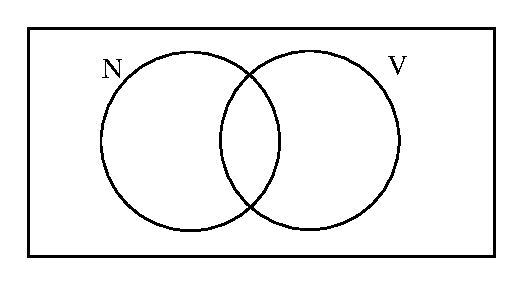
\includegraphics[width=12pc]{figures/algum.eps}}
\caption{Algum: $\text{N}\cap\text{V}\neq\varnothing$}
\end{figure}

\begin{figure}[H]
\centerline{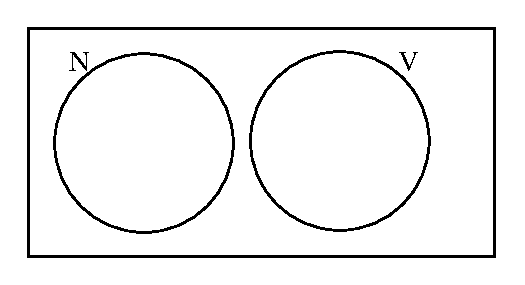
\includegraphics[width=12pc]{figures/nenhum.eps}}
\caption{Nenhum: $\text{N}\cap\text{V}=\varnothing$}
\end{figure}

\begin{figure}[H]
\centerline{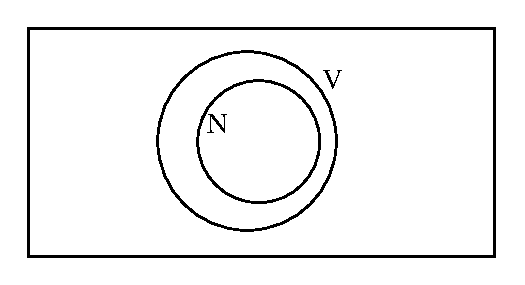
\includegraphics[width=12pc]{figures/todo.eps}} \caption{Todo:
$\text{N}\subseteq\text{V}$}
\end{figure}

\n Note agora uma característica das interpretações das sentenças
(\ref{rec})-(\ref{ree}) relacionada a suas representações acima.
Em todos os casos, para saber se a sentença é verdadeira, basta
perguntar quantos membros do conjunto N são também membros do
conjunto V. As respostas para os exemplos acima, claro, são: pelo
menos um, nenhum e todos, respectivamente. Em nenhum dos casos,
precisamos de informações sobre indivíduos que não pertencem ao
conjunto N. Isto significa que as extensões dos determinantes
acima podem ser caracterizadas levando-se em conta apenas os
conjuntos N e $\text{N}\cap\text{V}$, sem levar em conta os
membros de V que não pertencem a N ou os indivíduos que não
pertencem nem a N nem a V:


\begin{exe}
    \ex\label{lo}
    \begin{xlist}
        \ex  \den{algum}(N)(V) = 1 \textit{sse}
            $\text{N}\cap\text{V}\neq\varnothing$\label{loa}
        \ex  \den{nenhum}(N)(V) = 1 \textit{sse}
            $\text{N}\cap\text{V}=\varnothing$\label{loz}
        \ex  \den{todo}(N)(V) = 1 \textit{sse}
            $\text{N}=\text{N}\cap\text{V}$\label{loc}
    \end{xlist}
\end{exe}

\n Mas se os elementos de V que não estão na interseção com N são mesmo irrelevantes, poderíamos trocar V em (\ref{lo}a-c) por $N \cap V$ sem perda semântica. Considere, então, o que acontece se substituirmos o conjunto V
pelo conjunto $\text{N}\cap\text{V}$ nas condições acima:


\begin{exe}
    \ex\label{clu}
    \begin{xlist}
        \ex  \den{algum}(N)($\text{N}\cap\text{V}$) = 1 \textit{sse}
            $\text{N}\cap (\text{N}\cap\text{V})\neq\varnothing$\label{clua}
        \ex  \den{nenhum}(N)($\text{N}\cap\text{V}$) = 1 \textit{sse}
            $\text{N}\cap (\text{N}\cap\text{V})=\varnothing $\label{cluz}
        \ex  \den{todo}(N)($\text{N}\cap\text{V}$) = 1 \textit{sse}
            $\text{N}=\text{N}\cap (\text{N}\cap\text{V})$\label{cluc}
    \end{xlist}
\end{exe}


\n As condições de verdade acima parecem distintas das anteriores.
Entretanto, pelas definições da teoria dos conjuntos, sabemos que, para quaisquer conjuntos A e B, vale a seguinte equivalência:\\

\n $\text{A}\cap (\text{A}\cap\text{B})\ =\
\text{A}\cap\text{B}$\\

\n Isso nos permite simplificar as condições de verdade acima,
reduzindo-as ao seguinte:


\begin{exe}
    \ex\label{sel}
    \begin{xlist}
        \ex  \den{algum}(N)($\text{N}\cap\text{V}$) = 1 \textit{sse}
            $\text{N}\cap\text{V}\neq\varnothing$\label{sela}
        \ex  \den{nenhum}(N)($\text{N}\cap\text{V}$) = 1 \textit{sse}
            $\text{N}\cap \text{V}=\varnothing$\label{selz}
        \ex  \den{todo}(N)($\text{N}\cap\text{V}$) = 1 \textit{sse}
            $\text{N}=\text{N}\cap\text{V}$\label{selc}
    \end{xlist}
\end{exe}

\n Mas o que aparece à direita do conectivo \textit{sse} nas
condições em (\ref{sel}) é exatamente o que aparecia à direita desse
conectivo nas condições em (\ref{lo}). Isto quer dizer que:


\begin{exe}
    \ex\label{ul}
    \begin{xlist}
        \ex  \den{algum}(N)(V) = \den{algum}(N)($\text{N}\cap\text{V}$)\label{ula}
        \ex  \den{nenhum}(N)(V) = \den{nenhum}(N)($\text{N}\cap\text{V}$)\label{ulz}
        \ex  \den{todo}(N)(V) = \den{nenhum}(N)($\text{N}\cap\text{V}$)\label{ulc}
    \end{xlist}
\end{exe}

\n Equivalências como essas parecem valer
para todos os determinantes das línguas naturais. Elas podem ser expressas em português por esquemas como os mostrados abaixo, em que o símbolo $\equiv$ indica que duas sentenças são semanticamente equivalentes:\\

\n D NP VP $\equiv$ D NP é um NP que VP \\

\n Concretamente:\\

\n Alguma criança chorou $\equiv$ Alguma criança é uma criança que chorou\\

\n Nenhuma criança chorou $\equiv$ Nenhuma criança é uma criança que chorou\\

\n Toda criança chorou $\equiv$ Toda criança é uma criança que chorou\\ 

\n E são essas equivalências que estão no cerne da propriedade de
conservatividade, que definimos a seguir:\\

\begin{tcolorbox}[boxrule=0pt,sharp corners]

\n\textbf{Conservatividade}\\
Para qualquer determinante \textit{D} e quaisquer conjuntos
\textit{A} e \textit{B}, dizemos que \textit{D} é conservativo se,
e somente se, $\llbracket D \rrbracket(A)(B)= \llbracket D \rrbracket(A)(A\cap B)$

\end{tcolorbox}

\bigskip

\n Podemos, então, formular a seguinte hipótese para as línguas naturais:\\

\begin{tcolorbox}[boxrule=0pt,sharp corners]

\n\textbf{Universal da Conservatividade}\\
Todo determinante é conservativo.

\end{tcolorbox}

\bigskip


\n A validade desse universal é algo sujeito a confirmação
empírica. Como possível contraexemplo, considere o item
\textit{só} do português, que aparece em sentenças como (\ref{so})
abaixo:

\begin{exe}
    \ex Só crianças choram. \label{so}
\end{exe}

\n Note uma certa semelhança sintática dessa sentença com as que
analisamos mais acima. A palavra \textit{só} vem seguida de um NP
e o constituinte resultante é o sujeito do VP que o segue. Parece
que estamos, de fato, diante de um determinante. Pensemos agora
nas condições de verdade de (\ref{so}). Para que essa sentença
seja verdadeira, é preciso que ninguém além das crianças chore, ou seja, que todo indivíduo que chore seja uma
criança. Isto nos leva à seguinte entrada lexical para
\textit{só}:\\

\n \den{só} = $\lambda F_{\langle et\rangle}.\lambda G_{\langle
et\rangle}.\ \forall x [G'(x)\rightarrow F'(x)]$\\

\n Já na versão baseada em conjuntos que exploramos acima, podemos
caracterizar as condições de verdade de (\ref{so}) através do
diagrama abaixo:

\begin{figure}[H]
\centerline{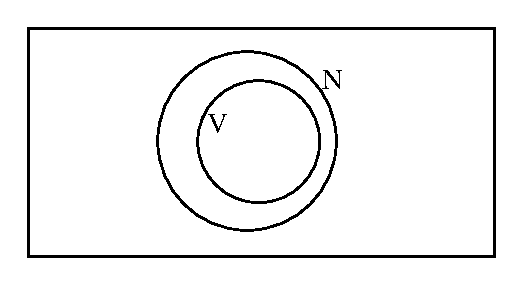
\includegraphics[width=12pc]{figures/so.eps}} \caption{Só:
$\text{V}\subseteq\text{N}$}
\end{figure}

\n Note que, para sabermos se (\ref{so}) é verdadeira, não basta
perguntarmos quantos elementos de N pertencem a V, ou seja, quantas crianças choram. Precisamos
também de informação sobre a existência ou não de elementos que
pertencem a V, mas não pertencem a N. Nesse aspecto, \textit{só}
difere dos determinantes que vimos anteriormente e essa diferença
é fruto do fato de que \textit{só} não é conservativo. 

Para provar a não conservatividade de \textit{só}, basta observar a não equivalência entre \textit{só crianças são crianças que choram} e \textit{só crianças choram}, em oposição à equivalência entre, por exemplo, \textit{toda criança é uma criança que chora} e \textit{toda criança chora}. De um ponto de vista mais formal, basta olharmos para
a caracterização de sua extensão na versão baseada em conjuntos:\\

\n \den{só}(N)(V) = 1 \textit{sse} $\text{V}\subseteq\text{N}$\\

\n Note que o que aparece do lado direito do conectivo
\textit{sse} é uma contingência, ou seja, algo que pode ser
verdadeiro ou falso dependendo da natureza de \textit{N} e
\textit{V}. Considere agora o que acontece se substituirmos
\textit{V} por
$\text{N}\cap\text{V}$:\\

\n \den{só}(N)($\text{N}\cap\text{V}$) = 1 \textit{sse}
$(\text{N}\cap\text{V})\subseteq\text{N}$\\

\n O que aparece agora após o conectivo \textit{sse} é uma
tautologia, já que, para quaisquer conjuntos \textit{N} e
\textit{V}, a interseção de \textit{N} e \textit{V} é um
subconjunto de N. A conclusão que tiramos disso é que as duas
condições de verdade acima não são equivalentes, e que, portanto,
\textit{só} não é conservativo.

Essa conclusão bastaria para refutarmos o Universal da
Conservatividade, não fosse o fato de que há sólidas evidências de
que \textit{só} não é um determinante. Ao contrário dos
determinantes que discutimos anteriormente, \textit{só} não
precede apenas NPs, mas também DPs, como em \textit{só o menino}
ou \textit{só algumas meninas}, VPs como em \textit{João só
dançou}, APs como em \textit{João está só triste} e PPs, como em
\textit{João viaja só de primeira classe}. Isto leva a crer que \textit{só} é
na verdade um tipo de adjunto que não é seletivo em relação à
categoria do constituinte ao qual se adjunge. Podemos assim manter
viva a hipótese de que determinantes são universalmente
conservativos.

Como já afirmamos acima, universais como esse são hipóteses a serem
confirmadas empiricamente, e uma das linhas de pesquisa abertas
pelo estudo formal das propriedades dos determinantes e dos
quantificadores generalizados que eles originam é justamente a
busca desses universais semânticos.

\section{Quantificação e escopo}

\subsection{DPs quantificadores em posição de objeto}

Todos os exemplos que analisamos até aqui neste capítulo continham
sintagmas quantificadores na posição de sujeito. Tal escolha não
se deu por acaso, e para entender o porquê de termos evitado
outras posições sintáticas, vamos considerar um exemplo com um DP
quantificador na posição de objeto direto de um verbo
transitivo, como em (\ref{tr}):

\begin{exe}
    \ex O João elogia todo professor. \label{tr}
\end{exe}

\n A extensão do verbo \textit{elogia} é de tipo $\langle
e,et\rangle$ e a do DP \textit{todo professor} de tipo $\langle
et,t\rangle$. Não há, portanto, como utilizar aplicação funcional
para obter a extensão do VP \textit{elogia todo professor}.
Outras regras composicionais que introduzimos, como
abstração funcional ou conjunção funcional,
também não nos servem. Essa situação contrasta com casos em que um
DP aparece na posição de sujeito como em (\ref{su}) abaixo, em que
a extensão do VP \textit{elogia o João} é de tipo $\langle e,t\rangle$ e pode servir de argumento para a extensão do DP
sujeito, como já vimos anteriormente:

\begin{exe}
    \ex Todo professor elogia o João. \label{su}
\end{exe}

\n Note que as condições de verdade tanto de (\ref{tr}) quanto de (\ref{su}) são intuitivamente claras e facilmente representáveis na notação que estamos adotando:

\begin{exe}

\ex \den{O João elogia todo professor} = 1 \textit{sse} \\
$\forall x [ \predica{professor}{x}\ \rightarrow\ \predica{elogia}{joão,x}]$ \label{comp1}

\ex \den{Todo professor elogia o João} = 1 \textit{sse} \\
$\forall x [\predica{professor}{x}\ \rightarrow\ \predica{elogia}{x,joão}]$ \label{comp2}

\end{exe}

\n Em ambos os casos, temos o prefixo quantificador $\forall x$ seguido de uma afirmação contendo a variável $x$. Essa afirmação, uma fórmula lógica, é o \textsc{escopo} de $\forall x$. A questão que nos resta é como obter composicionalmente essas condições de verdade no caso de (\ref{comp1}), a começar pelo problema da incompatibilidade de tipos que acabamos de ver.

Logo adiante, veremos como reformular nosso sistema interpretativo e tornar exemplos como (\ref{tr}) interpretáveis, derivando suas condições de verdade sem perder nada do que já obtivemos para casos como (\ref{su}). Antes, porém, vamos discutir dois fenômenos relacionados e que dizem respeito à maneira como DPs quantificadores interagem semanticamente entre si e com a negação.


\subsection{Interação de escopo entre DPs}


Vejamos agora casos em que mais de um DP
quantificador aparece na mesma sentença, como em
(\ref{int}), por exemplo:

\begin{exe}
    \ex Um parecerista anônimo revisará todo artigo que for submetido a esta revista.\label{int}
\end{exe}

\n A primeira coisa a se notar a respeito de
(\ref{int}) é que parecemos estar diante de uma sentença ambígua, que
admite duas interpretações. A primeira interpretação afirma a existência de um certo parecerista que fará a revisão de todos os artigos que forem submetidos ao periódico em questão. De acordo com essa interpretação, para que (\ref{int}) seja verdadeira, é preciso que um único parecerista seja responsável pela revisão de todos os artigos submetidos. Tal interpretação pode ser parafraseada por algo como: existe um parecerista \textit{x}, tal
que \textit{x} revisará todo artigo submetido ao periódico. Ou ainda, e de maneira um pouco mais prolixa: existe um parecerista \textit{x}, tal que, para todo artigo \textit{y} submetido ao periódico, \textit{x} revisará \textit{y}. Usando a notação que empregamos nas seções anteriores, podemos
representar abreviadamente essa interpretação da seguinte maneira:

\begin{exe}
    \ex $\exists x [\predica{parecerista}{x}\ \&\ 
    \forall y [\predica{artigo}{y} \rightarrow \predica{revisará}{x,y}]]$
     \label{qua}
\end{exe}


\n O que está escrito em (\ref{qua}) é que existe um indivíduo
\textit{x} que tem duas propriedades: \textit{x} é parecerista e \textit{x} revisará todo artigo em questão. 

Antes de prosseguir, vamos olhar mais atentamente para a estrutura
interna da representação formal em (\ref{qua}). Olhando de fora
para dentro, notamos que (\ref{qua}) tem a forma $\exists
x [\phi]$, em que $\phi$ é uma fórmula lógica. Essa fórmula é o
escopo do quantificador $\exists x$ introduzido pelo
determinante  \textit{um}. Note agora que no interior de $\phi$
está a contribuição do determinante \textit{todo}, que podemos representar esquematicamente por $\forall y [\psi]$, em que $\psi$ é também uma fórmula lógica. Em casos como esse, dizemos que o quantificador existencial introduzido pelo determinante \textit{um} tem escopo sobre o
quantificador universal introduzido pelo determinante \textit{todo}, ou, vendo de ângulo oposto, que o quantificador universal introduzido pelo determinante \textit{todo} está no escopo do
quantificador existencial introduzido pelo determinante \textit{um}. Pode-se dizer também que o DP sujeito tem escopo sobre o DP objeto.

Passemos agora para a segunda interpretação de (\ref{int}), um
pouco menos saliente que a primeira. De acordo com essa interpretação, todo artigo submetido ao periódico passará pela revisão de um parecerista, não necessariamente o mesmo. Tal interpretação não exige a existência de um certo parecerista que revise todos os artigos em questão. Exige-se apenas que, para todo artigo \textit{y}, exista um parecerista \textit{x}, tal que \textit{x} revise \textit{y}. Formalmente, temos o seguinte:

\begin{exe}
   \ex $\forall y [\predica{artigo}{y} \rightarrow \exists x [\predica{parecerista}{x}\ \&\ 
        \predica{revisará}{x,y}]]$
     \label{xa}
\end{exe}

\n A representação em (\ref{xa}) nos diz que para todo \textit{y}, se \textit{y} é um artigo, então existe um \textit{x}, tal que \textit{x} é um parecerista e \textit{x} revisará \textit{y}. Note
que, aqui, é o quantificador existencial $\exists$ que
aparece no interior da formula introduzida pelo quantificador
universal $\forall$. Dizemos nesse caso que o quantificador universal tem escopo sobre o existencial, ou ainda, que o DP
\textit{todo artigo submetido a este periódico} tem escopo sobre o DP
\textit{um parecerista}.

Analisando as interpretações de (\ref{qua}), deparamo-nos então
com uma \textsc{ambiguidade de escopo} e queremos que nosso sistema interpretativo consiga ajudar a explicá-la.

\subsection{Negação e escopo}

Passemos, agora, a um caso em que um DP quantificador interage com um outro tipo de operador, a negação. Considere a sentença abaixo:

\begin{exe}
    \ex João não elogia todo professor. \label{elo}
\end{exe}

\n Na interpretação mais natural desta sentença, para que ela seja
verdadeira é preciso que haja pelo menos um professor que o João
não elogie. Dito de maneira um pouco mais prolixa, é falso que para todo professor \textit{x}, o João elogia
\textit{x}. Podemos representar essas condições de verdade da
seguinte forma:

\begin{exe}
    \ex $\neg\forall x [\predica{professor}{x}\ \rightarrow\ \predica{elogia}{joão,x}]$ \label{wq}
\end{exe}

\n Para uma fórmula do tipo $\neg\phi$, em que $\phi$ também é uma
fórmula, dizemos que $\phi$ corresponde ao escopo do operador
negativo $\neg$. Para uma fórmula $\forall x [\phi]$, já vimos que $\phi$ é o escopo do quantificador universal $\forall$. Note que, em (\ref{wq}), o quantificador universal aparece no interior do
escopo do operador negativo. Dizemos, então, que a negação tem
escopo sobre o quantificador universal. Costuma-se dizer também que a negação tem escopo sobre o DP quantificador.

Já para uma interpretação de (\ref{elo}) em que o quantificador universal tivesse escopo sobre a negação, teríamos algo parafraseável como ``para todo professor \textit{x}, é falso que o João elogia \textit{x}''. Em termos formais:

\begin{exe}
    \ex $\forall x [\predica{professor}{x} \rightarrow\ \neg\predica{elogia}{joão,x}]$ \label{wqq}
\end{exe}


\n De acordo com (\ref{wqq}), (\ref{elo}) é verdadeira se, e somente se, para qualquer professor \textit{x}, não for verdade que João elogia \textit{x}, ou seja se, e somente se, João não elogiar nenhum professor. Essa parece ser uma interpretação bem menos saliente para (\ref{elo}) e talvez só seja possível quando o DP quantificador estiver bastante enfatizado. De qualquer forma, precisamos ver como nosso sistema interpreta estruturas em que DPs quantificadores e negação estão presentes em uma mesma estrutura.

Nas duas próximas seções, vamos apresentar e discutir, uma de cada vez, duas estratégias para lidar com as questões levantadas nessa seção a respeito da interpretação de DPs quantificadores e seu escopo relativo a outros constituintes sintáticos. A primeira delas é eminentemente sintática, mantendo nosso sistema interpretativo
intacto, mas operando transformações sobre a estrutura sintática das sentenças. Já a segunda, vai na direção oposta,
sendo eminentemente semântica. De acordo com ela, a estrutura
sintática relevante para sua interpretação é a estrutura superficial com DPs quantificadores ocupando as mesmas posições argumentais que DPs referenciais. Porém, os tipos semânticos atribuídos a alguns componentes
da sentença são modificados através de regras de mudanças de tipos. 

\section{Quantificação e movimento}

Voltemos ao caso dos DPs quantificadores em posição de objeto:

\begin{exe}
	\ex O João elogia todo professor. \label{etp}
\end{exe}

\n As condições de verdade dessa sentença exigem que, para todo indivíduo $x$, se $x$ for professor, então $x$ é elogiado pelo João. Na linha do que estamos vendo nesse capítulo, chegaríamos a esse resultado se fornecêssemos à extensão do determinante \textit{todo} funções que caracterizassem o conjunto dos indivíduos que são professores e o conjunto do indivíduos que João elogia. Quanto ao primeiro, não há problema: trata-se da extensão do NP complemento de D. Mas e o segundo? Eis o que queremos:\\

\n $\lambda x.\ \predica{elogia}{joão,x}$ \\
 

A primeira estratégia que veremos consiste em uma operação sintática de movimento. Nela, um DP quantificador se desloca para o topo de uma sentença, deixando para trás um vestígio. Esse DP movido e o seu vestígio recebem índices numéricos idênticos, como representado a seguir:\\


\begin{forest}
	[S$'$ 
	[DP$_1$[{todo professor},roof,name=subj]]
	[S
	[DP[{o Joao},roof]]
	[VP
	[V[elogia]]
	[t$_1$,name=vest]
	]
	]
	]
	\draw[->] (vest) to[out=south west,in=south] (subj);	
\end{forest}


\n Essa operação sintática é conhecida como \textsc{alçamento de
quantificador} (AQ) e tem como peculiaridade o fato de que não
afeta a maneira como pronunciamos a sentença, apenas a maneira
como a interpretamos. Em outras palavras, o resultado desta
operação não é visível para o componente fonológico da gramática, apenas
para o componente semântico.

A exemplo do que vimos quando discutimos a estrutura interna das
orações relativas, vamos assumir, \textit{a la} \cite{heikra98}, um processo de transferência de
índices na interface sintaxe-semântica, em que o índice do
constituinte movido é transferido desse para o constituinte que for seu
irmão.\\

\Tree [.S\2 \qroof{todo professor}.DP [.S\1 1 [.S \qroof{O
João}.DP [.VP [.V elogia ] t$_1$ ] ] ] ]

\bigskip

\n Portanto, para a interpretação de (\ref{etp}), é a estrutura
acima que o componente semântico recebe como \textit{input}.
Vejamos, agora, como nosso sistema interpreta essa estrutura. De
acordo com o que vimos no capítulo anterior, quando introduzimos a
regra de abstração funcional, temos que:\\

\n \den{S$'$}$^{g}$ = $\lambda x.\
\llbracket\text{S}\rrbracket^{g[1\rightarrow x]}$\\

\n Como sabemos que (consulte o capítulo anterior se você tiver dúvidas):\\

\n \den{S}$^{g[1\rightarrow x]}$ = 1 \textit{sse} $\predica{elogia}{joão,x}$\\

\n então,\\

\n \den{S$'$}$^{g}$ = $\lambda x.\ \predica{elogia}{joão,x}$\\

\n Isso é exatamente o que queríamos. Note que essa extensão é uma função de tipo $\langle
e,t\rangle$, que é o que a extensão do DP movido toma como
argumento. Podemos, então, utilizar aplicação funcional para obter a
extensão de $S''$:\\

\n\den{S$''$}$^{g}$ = \den{DP}$^{g}$(\den{S$'$}$^{g}$)\\

\n\den{DP}$^{g}$ = $\lambda F.\ \forall x [\predica{professor}{x} \rightarrow\ F'(x)]$\\

\n \den{S$''$}$^{g}$ = 1 \textit{sse} $\forall x [\predica{professor}{x} \rightarrow\ \predica{elogia}{joão,x}]$\\

\n Note que, como a extensão acima não depende da atribuição
\textit{g} (essa não aparece à direita de \textit{sse}), podemos,
de acordo com a convenção que adotamos no capítulo anterior,
escrever simplesmente:\\

\n \den{S$''$} = 1 \textit{sse} $\forall x [\predica{professor}{x} \rightarrow\ \predica{elogia}{joão,x}]$\\


\n Essas eram exatamente as condições de verdade que queríamos
derivar. Valendo-nos apenas dos princípios composicionais que já
tínhamos à nossa disposição, em particular aplicação e abstração funcional, conseguimos derivar o
significado de (\ref{etp}). O custo disso, claro, foi a postulação
de uma operação sintática (AQ) sem reflexos fonológicos.


\subsection{Movimento e escopo}

A regra de alçamento de quantificadores move um DP quantificador
para o topo da sentença, deixando em seu lugar de origem um
vestígio. Vamos aplicá-la agora ao exemplo com dois DPs quantificadores que vimos anteriormente e que repetimos em
(\ref{rt}):

\begin{exe}
    \ex Um parecerista (anônimo) revisará todo artigo (que for submetido a esta revista).  \label{rt}
\end{exe}

O alvo de AQ será o DP \textit{todo artigo}, o que resultará
na estrutura abaixo (já assumindo a transferência de índice):

\begin{exe}
	
	\ex \Tree [.S\2$_{t}$ \qroof{todo artigo}.DP\1$_{\langle et,t \rangle}$ [.S\1$_{\langle e,t \rangle}$ 1 [.S$_{t}$
	\qroof{um parecerista}.DP$_{\langle et,t \rangle}$ [.VP$_{\langle e,t \rangle}$ [.V$_{\langle e,et \rangle}$ revisará ] $t_{1_{e}}$ ] ] ] ]
	
\end{exe}

\bigskip

\n Nessa estrutura, foram anotados os tipos semânticos de todos os nós, de acordo com o previsto pelas entradas lexicais e as regras de aplicação funcional e abstração funcional. Note que não há incompatibilidades e que o nó raiz (S) é de tipo $t$, como deve ser. Vejamos, então, a interpretação que nosso sistema deriva para essa
estrutura, procedendo de cima para baixo. Omitiremos alguns passos, deixando-os a cargo do leitor.\\

\n \den{S$''$}$^{g}$ = \den{DP$'$}$^{g}$(\den{S$'$}$^{g}$)\hfill (AF)\\

\n \den{DP$'$}$^{g}$ = $\lambda F.\ \forall x [\predica{artigo}{x}\ \rightarrow\ F'(x)]$\\

\n \den{S$''$}$^{g}$ = 1 \textit{sse}  $\forall x [\predica{artigo}{x} \rightarrow\ \llbracket\text{S}'\rrbracket^{g}(x)=1]$\\

\n Para o nó S$'$, usamos abstração funcional:\\

\n \den{S$'$}$^{g}$ = $\lambda z.\
\llbracket\text{S}\rrbracket^{g[1\rightarrow z]}$\\

\n Para evitar confusões nos processos de conversão-$\lambda$ durante a derivação, usamos aqui a variável $z$, já que $x$ e $y$ aparecerão em outros momentos da derivação. Trata-se, entretanto, da mesmíssima regra com a qual já estamos familiarizados. Para o nó S, voltamos a utilizar aplicação funcional:\\

\n \den{S}$^{g[1\rightarrow z]}$ = \den{DP}$^{g[1\rightarrow
z]}$(\den{VP}$^{g[1\rightarrow z]}$) \\

\n \den{DP}$^{g[1\rightarrow z]}$ = $\lambda F.\
\exists y [\predica{parecerista}{y}\ \&\ F'(y)]$\\

\n Por fim, para o nó VP, teremos, via aplicação funcional:\\

\n \den{VP}$^{g[1\rightarrow z]}$ = \den{V}$^{g[1\rightarrow z]}$(\den{t$_{1}$}$^{g[1\rightarrow z]}$)\\

\n \den{V}$^{g[1\rightarrow z]}$ = $\lambda v.\lambda w.\ \predica{revisará}{w,v}$\\

\n \den{t$_{1}$}$^{g[1\rightarrow z]}$ = $g[1\rightarrow z](1)$ = $z$\\

\n Note o uso na representação da extensão de V das variáveis $v$ e $w$, diferentes das já utilizadas mais acima. Aqui também o intuito é manter a clareza na exposição da derivação.

Tendo chegado à parte de baixo da estrutura, basta percorrermos o sentido inverso, efetuando as devidas conversões: \\

\n \den{VP}$^{g[1\rightarrow z]}$ = $\lambda w.\ \predica{revisará}{w,z}$\\

\n \den{S}$^{g[1\rightarrow z]}$ = 1 \textit{sse} $\exists y [\predica{parecerista}{y}\ \&\ \predica{revisará}{y,z}]$\\

\n \den{S$'$}$^{g}$ = $\lambda z.\ \exists y [\predica{parecerista}{y}\ \&\ \predica{revisará}{y,z}]$\\

\n \den{S$''$}$^{g}$ = 1 \textit{sse} $\forall x [\predica{artigo}{x} \rightarrow \exists y [\predica{parecerista}{y}\ \&\ \predica{revisará}{y,x}]]$\\

\n O que as condições acima requerem é que todo artigo seja revisado por um parecerista, não necessariamente o mesmo. Isso corresponde exatamente à leitura que discutimos na seção anterior em
que o DP \textit{todo artigo} tem escopo sobre o DP
\textit{um parecerista}. De fato, se compararmos as condições de verdade
acima com a representação que atribuímos a essa leitura anteriormente em
(\ref{xa}), notaremos que elas são idênticas, exceto pelas escolhas das variáveis, o que é irrelevante.

Derivamos, assim, uma das interpretações de (\ref{rt}). Mas, e a
outra, que afirma a existência de um certo parecerista que revisará todos os artigos em questão? Note que, na estrutura que gerou as condições de verdade
que acabamos de derivar, o DP \textit{todo artigo} aparece em
uma posição hierarquicamente superior ao DP \textit{um parecerista},
resultando na leitura em que o primeiro tem escopo
sobre o segundo. Para obtermos a leitura em que
\textit{um parecerista} tem escopo sobre \textit{todo artigo}, vamos
aplicar AQ novamente, desta vez movendo o DP \textit{um parecerista}
por sobre o DP \textit{todo artigo}. Isto resultará na seguinte
estrutura:\\



\begin{forest}
	[S$''''$ 
	[DP[{um parecerista},roof,name=um]]
	[S$'''$
	[2]
	[S$''$
	[DP$'$[{todo artigo},roof,name=todo]]
	[S$'$
	[1]
	[S
	[t$_2$,name=t2]
	[VP
	[V[revisará]]
	[t$_1$,name=t1]
	]
	]
	]
	]
	]
	]
	\draw[->] (t1) to[out=south west,in=south] (todo);
	\draw[->] (t2) to[out=south west,in=south] (um);
\end{forest}



\n Vejamos, então, que condições de verdade nosso sistema deriva
para essa estrutura. Procure acompanhar atentamente cada passo da derivação:\\

\n \den{S$''''$}$^{g}$ = \den{DP}$^{g}$(\den{S$'''$}$^{g}$)\hfill (AF)\\

\n \den{S$'''$}$^{g}$ = $\lambda x.\
\llbracket\text{S}''\rrbracket^{g[2\rightarrow x]}$ \hfill (Abs.F)\\

\n \den{S$''$}$^{g[2\rightarrow x]}$ = \den{DP$'$}$^{g[2\rightarrow
x]}$(\den{S$'$}$^{g[2\rightarrow x]}$)\hfill (AF)\\

\n \den{S$'$}$^{g[2\rightarrow x]}$ = $\lambda y.\
\llbracket\text{S}\rrbracket^{g[2\rightarrow x][1\rightarrow y]}$ \hfill (Abs.F)\\

\n \den{S}$^{g[2\rightarrow x][1\rightarrow y]}$ = \den{V}$^{g[2\rightarrow x][1\rightarrow y]}$(\den{t$_{1}$}$^{g[2\rightarrow x][1\rightarrow y]}$)(\den{t$_{2}$}$^{g[2\rightarrow x][1\rightarrow y]}$)  \hfill (Abs.F)\\

\n \den{S}$^{g[2\rightarrow x][1\rightarrow y]}$ = 1 \textit{sse}
$\predica{revisará}{x,y}$\\

\n \den{S$'$}$^{g[2\rightarrow x]}$ = $\lambda y.\ \predica{revisará}{x,y}$\\

\n \den{S$''$}$^{g[2\rightarrow x]}$ = \den{DP$'$}$^{g[2\rightarrow
x]}$($\lambda y.\ \predica{revisará}{x,y}$)\\

\n \den{DP$'$}$^{g[2\rightarrow x]}$ = $\lambda F.\ \forall y [\predica{artigo}{y} \rightarrow F'(y)]$\\

\n \den{S$''$}$^{g[2\rightarrow x]}$ = 1 \textit{sse} $\forall y [\predica{artigo}{y} \rightarrow\ \predica{revisará}{x,y}]$\\

\n \den{S$'''$}$^{g}$ = $\lambda x_{e}.\ \forall y [\predica{artigo}{y} \rightarrow\ \predica{revisará}{x,y}]$\\

\n \den{S$''''$}$^{g}$ = \den{DP}$^{g}$($\lambda x.\ \forall y [\predica{artigo}{y} \rightarrow\ \predica{revisará}{x,y}]$)\\

\n \den{DP}$^{g}$ = $\lambda F.\
\exists x [\predica{parecerista}{x}\ \&\ F'(x)]$\\

\n \den{S$''''$}$^{g}$ = 1 \textit{sse} $\exists x [\predica{parecerista}{x}\ \&\ \forall y [\predica{artigo}{y} \rightarrow\ \predica{revisará}{x,y}]]$\\

\n Se compararmos essas condições de verdade com a representação
em (\ref{qua}) apresentada originalmente, veremos que elas são idênticas.
Conseguimos, assim, captar a leitura de (\ref{rt}) em que
\textit{um parecerista} tem escopo sobre \textit{todo artigo}.

Podemos concluir que a regra sintática AQ permite gerar duas
estruturas sintáticas para (\ref{rt}) e que a interpretação de
cada uma delas resulta em uma das leituras associadas a essa
sentença. Explicamos, assim, a ambiguidade de (\ref{rt}),
reduzindo-a a um caso de ambiguidade sintática, em que à mesma
sentença (entendida como uma sequência de palavras) atribuímos
duas estruturas distintas. O custo disso, voltamos a repetir, é a postulação de um nível de representação sintática abstrato e que não corresponde à estrutura superficial da sentença no que diz respeito à posição dos DPs quantificadores.

Cumpre notar também que não impusemos nenhuma restrição a AQ relacionada à natureza dos DPs quantificadores alvejados por ela. Dessa forma, prevemos que sempre que houver dois ou mais deles em uma mesma oração, haverá ambiguidade. Essa liberdade acaba sendo problemática na medida em que certas combinações de DPs não admitem múltiplas interpretações. Considere, por exemplo, o caso abaixo:

\begin{exe}

	\ex Todo mundo resolveu menos de três questões. \label{glu}	
	
\end{exe}

\n Intuitivamente, a única leitura admissível para essa sentença é a de que para todo $x$, $x$ resolveu menos de três questões. Em outras palavras, não deve haver ninguém que tenha resolvido três ou mais questões. Essa é a interpretação em que o quantificador universal introduzido por \textit{todo mundo} tem escopo largo, que inclui a contribuição semântica do DP objeto e que pode ser obtida alçando-se esse último para uma posição sintática subordinada à do DP sujeito:

\begin{exe}
	\ex $[$ Todo mundo 1 [ menos de três questões 2 [ t$_{1}$ resolveu t$_{2}$]]]	
\end{exe}

Considere, agora, a estrutura resultante do movimento do DP objeto para uma posição acima da do DP sujeito:

\begin{exe}
	\ex $[$ menos de três questões 2 [ todo mundo  resolveu t$_{2}$]]	
\end{exe}

\n Nesse caso, teremos uma inversão de escopo e a interpretação resultante será a de que menos de três questões foram resolvidos por todo mundo. Mas essa não é uma interpretação que (\ref{glu}) tem. Pensemos um pouco mais a respeito. Imagine, por exemplo um cenário com 5 pessoas (p$_{1}$-p$_{5}$), cinco questões (q$_{1}$-q$_{5}$) e  os fatos relevantes representados na tabela abaixo:\\

\n \begin{tabular}{c|c}
	\hline 
	\textbf{pessoas} & \textbf{questões resolvidas} \\ 
	%\hline 
	p$_{1}$ &  q$_{1}$,q$_{2}$,q$_{3}$,q$_{4}$,q$_{5}$\\ 
	%\hline 
	p$_{2}$ &  q$_{1}$,q$_{2}$\\ 
	%\hline 
	p$_{3}$ &  q$_{1}$,q$_{2}$,q$_{4}$\\ 
	%\hline 
	p$_{4}$ &  q$_{1}$,q$_{2}$,q$_{5}$\\ 
	%\hline 
	p$_{5}$ &  q$_{1}$,q$_{2}$,q$_{3}$,q$_{4}$\\ 
	\hline 
\end{tabular} \\

\n Nesse cenário, é falso que todo mundo tenha resolvido menos de três questões. p$_{1}$, por exemplo, resolveu todas as cinco. Mas é verdadeiro que menos de três questões tenham sido resolvidas por todo mundo (apenas duas, q$_{1}$ e q$_{2}$, foram). Se a inversão de escopo fosse possível, (\ref{glu}) deveria ser julgada verdadeira nessas circunstâncias. Como esse não é o caso, concluímos que essa inversão não é possível.

Além disso, parece haver diferenças translinguísticas em alguns casos. O português brasileiro, por exemplo, parece bastante rígido em relação à possibilidade de inversão de escopo. Mesmo em sentenças como as que vimos anteriormente, envolvendo quantificadores universal e existencial, tal inversão parece bem pouco saliente. Deixaremos essas observações como um alerta para o leitor. De alguma forma, AQ (ou qualquer operação que seja responsável pelo movimento dos DPs quantificadores) precisa ter seu papel regulado, com o movimento sintático em questão afetando de maneira distinta,  diferentes tipos de DPs quantificadores. Remetemos o leitor a algumas das sugestões de leitura oferecidas ao final do capítulo. 



\subsection{Negação e alçamento de quantificadores}

Considere novamente a sentença abaixo:

\begin{exe}
    \ex João não elogia todo professor. \label{eloi}
\end{exe}

\n Conforme já discutimos, a interpretação mais natural dessa sentença exige que
seja falso que João elogie todo professor. Vejamos se nosso sistema consegue derivar as condições de
verdade almejadas. Já sabemos que para interpretar um DP
quantificador na posição de objeto direto, precisamos movê-lo para
o topo da sentença. Isso nos fornece a seguinte
estrutura:\\

\Tree [.S\2 \qroof{todo professor}.DP [.S\1 1 [.S
\qroof{João}.DP$'$ [.VP$'$ não [.VP [.V elogia ] t$_1$ ] ] ] ] ]

\bigskip

\n Calculemos as condições de verdade dessa estrutura:\\

\n\den{S$''$}$^{g}$ = \den{DP}$^{g}$(\den{S$'$}$^{g}$)\\

\n \den{S$'$}$^{g}$ = $\lambda x_{e}.\
\llbracket\text{S}\rrbracket^{g[1\rightarrow x]}$\\

\n \den{S}$^{g[1\rightarrow x]}$ = \den{VP$'$}$^{g[1\rightarrow
x]}$(\den{DP$'$})$^{g[1\rightarrow x]}$\\

\n \den{VP$'$}$^{g[1\rightarrow x]}$ = \den{não}$^{g[1\rightarrow
x]}$(\den{VP}$^{g[1\rightarrow x]}$)\\

\n \den{VP}$^{g[1\rightarrow x]}$ = \den{V}$^{g[1\rightarrow
x]}$(\den{t$_{1}$}$^{g[1\rightarrow x]}$)\\

\n \den{V}$^{g[1\rightarrow x]}$ = $\lambda x.\lambda y.\ \predica{elogia}{y,x}$\\

\n \den{t$_{1}$}$^{g[1\rightarrow x]}$ = $x$\\

\n \den{VP}$^{g[1\rightarrow x]}$ = $\lambda y.\ \predica{elogia}{y,x}$\\

\n \den{não}$^{g[1\rightarrow x]}$ = $\lambda F.\ \lambda z.\ \neg F'(z)$\\

\n \den{VP$'$}$^{g[1\rightarrow x]}$ = $\lambda z.\ \neg\predica{elogia}{z,x}$\\

\n \den{DP$'$}$^{g[1\rightarrow x]}$ = \textit{joão}\\

\n \den{S}$^{g[1\rightarrow x]}$ = 1 \textit{sse}  $\neg\predica{elogia}{joão,x}$\\

\n \den{S$'$}$^{g}$ = $\lambda x.\ \neg\predica{elogia}{joão,x}$\\

\n \den{DP}$^{g}$ = $\lambda F.\ \forall x [\predica{professor}{x} \rightarrow F'(x)]$\\

\n \den{S$''$}$^{g}$ = 1 \textit{sse} $\forall x [\predica{professor}{x} \rightarrow \neg\predica{elogia}{joão,x}]$\\

\n O que essas condições de verdade requerem é que, para todo
professor \textit{x}, o João não elogie \textit{x}, ou seja, que o
João não elogie nenhum professor. Conforme já salientamos, essa interpretação, se é que
existe, é bem menos saliente que a interpretação de acordo com a qual se nega apenas que o João elogie todo e qualquer professor. O problema com as condições que
acabamos de derivar é que, de acordo com elas, o quantificador
universal tem escopo sobre a negação, enquanto o que queríamos
era que a negação tivesse escopo sobre o quantificador universal.

Mas como obter a interpretação de (\ref{eloi}) que desejamos?
Dado o que já vimos sobre interação de escopo na seção anterior, a
resposta parece simples: basta mover o DP \textit{todo professor}
para uma posição abaixo da negação. Vejamos se isso realmente
funciona. A estrutura que obteríamos seria a seguinte:\\

\Tree [.S \qroof{João}.DP [.VP$'''$ não [.VP\2 \qroof{todo
professor}.DP\1 [.VP\1 1 \qroof{elogia t$_{1}$}.VP ] ] ] ]

\bigskip

\n O problema é que essa estrutura não é interpretável. A extensão
de VP é de tipo $\langle e,t\rangle$. Com isso, a extensão de VP$'$
será de tipo $\langle e,et\rangle$, em razão da regra de abstração funcional. Como a extensão de
\textit{todo professor} é de tipo $\langle et,t\rangle$, não há
como derivar a extensão de VP$''$ e, por conseguinte, de nenhum nó
acima dele, incluindo o nó-raiz S. Note que, para tornar VP$''$
interpretável, bastaria que a extensão de VP$'$ fosse de tipo
$\langle e,t\rangle$ e que dessa forma pudesse servir de argumento
para a extensão de \textit{todo professor}. Mas, para isso, a
extensão de VP precisaria ser de tipo \textit{t}, o que
exigiria que o sujeito fosse interpretado no interior de VP,
saturando assim a extensão do verbo \textit{elogiar}.

Para implementar essa possibilidade, vamos nos valer daquilo que,
dentro do quadro teórico conhecido como \textsc{Teoria da regência e
ligação}, é chamado de \textsc{hipótese do sujeito interno a
VP} (ver referências ao final do capítulo). De acordo com essa hipótese, o sujeito de uma sentença é
gerado no interior de VP, movendo-se depois para a posição que
ocupa na estrutura superficial da sentença. Assim como nos outros
casos envolvendo movimento que já estudamos, vamos assumir que, ao se mover, o DP sujeito recebe um índice e deixa em sua posição de
origem um vestígio coindexado. Após o processo da transferência de
índice, obtém-se então a seguinte estrutura:\\


\begin{forest}
	for tree={s sep=10mm, inner sep=0, l=0}
	[S
	[DP$_{suj}$,name=subj]
	[$\alpha$
	[i]
	[\ldots
	[\ldots]
	[VP,circle,draw,fill=lightgray
	[t$_i$,name=vest]
	[V$'$
	[V]
	[DP$_{obj}$]
	]
	]
	]
	]
	]
	\draw[->] (vest) to[out=south west,in=south] (subj);	
\end{forest}

\bigskip

\n Vamos aplicar essas ideias ao nosso exemplo. Primeiramente, movemos o sujeito para sua posição superficial:\\


\begin{forest}
	for tree={s sep=10mm, inner sep=0, l=0}
	[S
	[João,name=subj]
	[$\alpha$
	[1]
	[VP
	[não]
	[VP
	[t$_1$,name=vest]
	[V$'$ [elogia todo professor, roof]]
	]
	]
	]
	]
	\draw[->] (vest) to[out=south west,in=south] (subj);	
\end{forest}

\bigskip

Em seguida, movemos o DP objeto para a posição imediatamente abaixo da negação:\\

\begin{forest}
	for tree={s sep=10mm, inner sep=0, l=0}
	[S
	[João,name=subj]
	[$\alpha$
	[1]
	[VP
	[não]
	[VP
	[DP [todo \\ professor, roof, name=todo]]
	[$\beta$
	[2]
	[VP [t$_1$ elogia t$_2$, roof,name=VP]]
	]
	]
	]
	]
	]
	\draw[->] (VP) to[out=west,in=south] (subj);
	\draw[->] (VP) to[out=east,in=south] (todo);	
\end{forest}

\bigskip


\n Eis os principais passos da derivação das condições
de verdade dessa estrutura:\\

\n \den{S}$^{g}$ = \den{1 não todo professor 2 VP}$^{g}$(\textit{joão})\\

\n \den{1 não todo professor 2 VP}$^{g}$ = $\lambda x.\
\llbracket \text{não todo professor 2 VP}\  \rrbracket^{g[1\rightarrow x]}$\\

\n \den{não todo professor 2 VP}$^{g[1\rightarrow x]}$ = \den{não}$^{g[1\rightarrow
x]}$(\den{todo professor 2 VP})$^{g[1\rightarrow x]}$\\

\n \den{todo professor 2 VP}$^{g[1\rightarrow x]}$ = \den{todo
professor}$^{g[1\rightarrow
x]}$(2 VP)$^{g[1\rightarrow x]}$\\

\n \den{2 VP}$^{g[1\rightarrow x]}$ = $\lambda y.\
\llbracket\text{VP}\rrbracket^{g[1\rightarrow x][2\rightarrow y]}$\\

\n \den{VP}$^{g[1\rightarrow x][2\rightarrow y]}$ = 1 \textit{sse}
$\predica{elogia}{x,y}$\\

\n Note que a extensão de VP é de tipo \textit{t}.
Efetuando-se as devidas substituições e conversões-$\lambda$,
obteremos o seguinte:\\

\n \den{2 VP}$^{g[1\rightarrow x]}$ = $\lambda y.\ \predica{elogia}{x,y}$\\

\n \den{todo professor 2 VP}$^{g[1\rightarrow x]}$ = 1 \textit{sse} $\forall y [\predica{professor}{y} \rightarrow \predica{elogia}{x,y}]$\\

\n Essa última extensão é de tipo $t$. Portanto, para a negação,
deve-se usar a versão de tipo $\langle t,t\rangle$, de acordo com a
entrada lexical que propusemos no capítulo 3:\\

\n \den{não} = $(\lambda p.\ p=0)$ \\

\n Prosseguindo, teremos:\\

\n \den{não todo professor 2 VP}$^{g[1\rightarrow x]}$ = ($\lambda p.\ p=0$)(\den{todo professor 2 VP})$^{g[1\rightarrow x]}$\\

\n \den{não todo professor 2 VP}$^{g[1\rightarrow x]}$ = 1 \textit{sse} \den{todo professor 2 VP}$^{g[1\rightarrow x]}$ = 0\\

\n \den{não todo professor 2 VP}$^{g[1\rightarrow x]}$ = 1 \textit{sse} $\neg\forall y [\predica{professor}{y} \rightarrow \predica{elogia}{x,y}]$\\

\n \den{1 não todo professor 2 VP}$^{g}$ = $\lambda x.\ \neg\forall y [\predica{professor}{y} \rightarrow \predica{elogia}{x,y}]$\\

\n \den{S} = 1 \textit{sse} $\neg\forall y [\predica{professor}{y} \rightarrow \predica{elogia}{joão,y}]$\\

\n Essas são exatamente as condições que queríamos derivar, com a negação tendo escopo sobre o quantificador universal. Novamente, valemo-nos de operações de movimento sintático que preparam, por assim dizer, a estrutura sintática para a interpretação baseada apenas em aplicação e abstração funcional, sem necessidade de rever os tipos semânticos dos constituintes envolvidos.


\section{Quantificação e mudança de tipos}

Vejamos, agora, uma segunda estratégia para a interpretação de
sentenças com DPs quantificadores em diversas posições sintáticas. Como anunciamos mais acima, essa estratégia mantém a
estrutura sintática superficial da sentença inalterada, sem alçamento de DPs quantificadores ou vestígio de sujeito interno a VP. No caso de \textit{O João elogia todo professor}, por exemplo, o que o componente semântico recebe para interpretar é a
estrutura abaixo:\\

\Tree [.S \qroof{O João}.DP [.VP [.V elogia ] \qroof{todo
professor}.DP ] ]

\bigskip

\n Para evitarmos a incompatibilidade de tipos que já detectamos
entre as extensões de V e do DP objeto, precisamos alterar pelo
menos uma dessas extensões, ou então criarmos um novo princípio
composicional. Vamos aqui implementar a primeira possibilidade, alterando o tipo semântico dos verbos.

Já notamos no início deste capítulo que, do ponto de vista
sintático, existe uma semelhança na distribuição de expressões
referenciais como nomes próprios e a distribuição de DPs
quantificadores, ambos ocupando as mesmas posições junto aos
predicados a eles relacionados. A ideia por trás da implementação
que vamos desenvolver aqui é a de que as extensões dos predicados
estão em sintonia com esses fatos e que regras semânticas podem
alterar o tipo dessas extensões, de modo a
torná-las aptas a tomar não só indivíduos (tipo $e$) mas
também quantificadores generalizados (tipo $\langle et,t\rangle$)
como argumentos. De maneira mais concreta, isso significa que há
regras que relacionam sistematicamente predicados de indivíduos e
predicados de quantificadores generalizados. Vamos aqui tomar os primeiros como básicos e derivar a extensão dos últimos elevando o tipo semântico de seus argumentos de $e$ para $\langle et,t\rangle$ quando necessário. Chamaremos essa regra de \textsc{Elevação de Argumento} (EA).\\

\begin{tcolorbox}[boxrule=0pt,sharp corners]

\n \textbf{Elevação de argumento (EA)}

\n Seja \textit{X} um constituinte cuja extensão $\alpha$ é
de tipo $\langle a_{1},...\langle a_{k},...\langle a_{n},t\rangle...\rangle\rangle$, com $n \geq 1$ e $a_{k} = e$. Mude a extensão de
\textit{X} de $\alpha$ para $\alpha '$, mudando $a_{k}$ de $e$ para $\langle et,t\rangle$ e definindo $\alpha '$ da seguinte forma:\\

\n $\alpha ' = \lambda x_{1}...\lambda Q_{\langle et,t\rangle}...\lambda x_{n}.\
Q(\lambda x_{k}.\ \alpha(x_{1})...(x_{k})...(x_{n}))$

\end{tcolorbox}

\n A regra acima aplica-se a funções com \textit{n} argumentos $x_{1},...,x_{k},...,x_{n}$, sendo o k-ésimo desses argumentos ($x_{k}$) de tipo \textit{e}. A regra modifica o tipo desse k-ésimo argumento, passando-o de $e$ para $\langle et,t\rangle$. É esse novo argumento \textit{Q} que será fornecido por um DP quantificador ocupando uma posição argumental. Vejamos um exemplo concreto com o verbo transitivo \textit{elogiar}. A extensão desse verbo é uma função de tipo $\langle e,et\rangle$, que toma dois argumentos de tipo \textit{e}. No esquema acima, portanto, $n=2$ e tanto $a_{1}$ quanto $a_{2}$ são iguais a \textit{e}. Vamos aplicar EA, tomando \textit{k} como sendo igual a $1$, e portanto, $x_{k}$ como sendo o primeiro argumento, que corresponde à posição de objeto direto. Esse argumento terá seu tipo elevado de $e$ para $\langle et,t\rangle$. A nova extensão do verbo será, portanto, de tipo $\langle \langle et,t\rangle,et\rangle$. Lembremos que a extensão original do verbo \textit{elogiar}, de tipo $\langle e,et\rangle$, é:\\

\n $\llbracket \text{elogia}_{1} \rrbracket = \lambda x.\lambda y.\ \predica{elogia}{y,x}$\\

\n Marcamos o verbo com um subscrito para diferenciar a extensão original da nova extensão que obteremos, aplicando a mudança de tipos especificada acima:\\

\n $\llbracket \text{elogia}_{2} \rrbracket = \lambda Q_{\langle et,t\rangle}.\lambda y.\
Q(\lambda x.\ \llbracket \text{elogia}_{1} \rrbracket (x)(y))$\\

\n Efetuando as conversões lambda, teremos:\\

\n $\llbracket \text{elogia}_{2} \rrbracket = \lambda Q_{\langle et,t\rangle}.\lambda y.\
Q(\lambda x.\ \predica{elogia}{y,x})$\\

\n Com essa nova extensão, o verbo \textit{elogiar} está apto a se combinar com um DP quantificador na posição de objeto, resultando em um VP cuja extensão terá o tipo $\langle e,t\rangle$, conforme se pode ver na derivação abaixo para a sentença \textit{João elogia todo professor}. Para o DP objeto, temos:\\

\n \den{DP} = $\lambda F.\ \forall z [\predica{professor}{z} \rightarrow\ F'(z)]$\\

\n Sendo a nova extensão do verbo de tipo $\langle \langle et,t\rangle,et\rangle$, podemos utilizar aplicação funcional para obter a
extensão do VP \textit{elogia todo professor}:\\

\n \den{VP} = \den{elogia$_{2}$}(\den{DP})\\

\n \den{VP} = ($\lambda Q_{\langle et,t\rangle}.\lambda y.\
Q(\lambda x.\ \predica{elogia}{y,x})$)(\den{DP})\\

\n Basta, agora, efetuar uma série de substituições e conversões-$\lambda$:\\

\n \den{VP} = $\lambda y.\ \llbracket \text{DP} \rrbracket(\lambda x.\ \predica{elogia}{y,x})$\\

\n \den{VP} = $\lambda y.\ (\lambda F.\
\forall z [\predica{professor}{z} \rightarrow F'(z)])(\lambda
x.\ \predica{elogia}{y,x})$\\

\n \den{VP} = $\lambda y.\ \ \forall z [\predica{professor}{z} \rightarrow\ (\lambda x.\ \predica{elogia}{y,x})(z)]$\\

\n \den{VP} = $\lambda y.\ \forall z [\predica{professor}{z} \rightarrow\ \predica{elogia}{y,z}]$\\

\n Essa extensão de VP é uma função que toma como argumento um indivíduo $y$ e retorna o valor de verdade 1 se, e somente se, $y$ elogia todo professor. Aplicando-a à extensão do DP sujeito \textit{João}, temos:\\

\n \den{S} = \den{VP}(\den{DP})\\

\n \den{DP} = \textit{joão}\\

\n \den{S} = 1 \textit{sse} $\forall z [\predica{professor}{z} \rightarrow\ \predica{elogia}{joão,z}]$\\

\n Essas são, de fato, as condições de verdade que desejávamos. Ao
contrário do que ocorreu com a primeira estratégia baseada em
movimento, desta vez não lançamos mão de nenhuma operação sintática nos moldes de AQ. O custo para mantermos nossa sintaxe
intacta foi a introdução de uma nova regra de mudança de tipos.

Não é óbvio como decidir entre as estratégias descritas acima nem do ponto de vista empírico nem do ponto de vista metodológico. Ambas, no intuito de dar conta da interpretação de sentenças com quantificadores na posição de objeto, complicam, por assim dizer, um dos componentes da gramática. A primeira, complica o componente sintático, e a segunda, o semântico. Deixaremos essa escolha em aberto.

\subsection{Mudança de tipos e escopo}

Vejamos, agora, como a abordagem acima, que dispensa o uso de movimento
sintático, lida com os fenômenos da ambiguidade de escopo entre DPs e da interação entre
a negação e DPs quantificadores. Voltemos ao exemplo \textit{Um parecerista (anônimo) revisará todo artigo (que for submetido a este periódico)} e sua estrutura superficial abreviada, dada abaixo:\\

\Tree [.S  \qroof{um parecerista}.DP [.VP [.V revisará ]  \qroof{todo artigo}.DP  ] ]

\bigskip

\n Na seção anterior, aplicamos a regra de mudança de tipos que chamamos de Elevação de Argumento (EA) a um verbo transitivo, mudando o tipo semântico do primeiro argumento de sua extensão de $e$ para $\langle et,t\rangle$. Isso possibilitou à nova extensão do verbo combinar-se diretamente com a extensão do seu objeto direto quantificado via aplicação funcional, resultando em uma extensão de tipo $\langle e,t\rangle$ para o sintagma verbal VP. Se adotarmos o mesmo procedimento com o verbo \textit{revisará} no exemplo acima, obteremos resultado análogo:\\

\n \den{revisará$_{2}$} = $\lambda Q_{\langle et,t\rangle}.\lambda y.\
Q(\lambda x.\ \predica{revisará}{y,x})$\\

\n Essa extensão tomará a extensão do DP objeto como argumento, via aplicação funcional:\\

\n \den{VP} = \den{revisará$_{2}$}(\den{todo artigo})\\

\n \den{todo artigo} = $\lambda F_{\langle et\rangle}.\ \forall z [\predica{artigo}{z}\ \rightarrow\ F'(z)]$\\

\n \den{VP} = $\lambda y.\ \forall z [\predica{artigo}{z} \rightarrow \predica{revisará}{y,z}]$\\

\n Como a extensão do DP sujeito é de tipo $\langle et,t\rangle$, ela pode tomar a extensão do VP como argumento. Utilizando, portanto, aplicação funcional, obtemos as condições de verdade para a sentença S:\\

\n \den{S} = \den{um parecerista}(\den{VP})\\

\n \den{um parecerista} = $\lambda F.\ \exists x [\predica{parecerista}{x}\ \&\ F'(x)]$\\

\n \den{S} = 1 \textit{sse} $\exists x [\predica{parecerista}{x}\ \&\ \forall z [\predica{artigo}{z} \rightarrow \predica{revisará}{x,z}]]$\\

\n Como se pode notar nessa representação das condições de verdade, o quantificador existencial tem escopo sobre o quantificador universal e a interpretação resultante é a de que um mesmo parecerista revisará todos os artigos em questão. Falta-nos agora obter a outra interpretação, que traz uma inversão de escopo, ou seja, o quantificador universal introduzido pelo DP objeto passa a ter escopo sobre o quantificador existencial introduzido pelo DP sujeito. Para tanto, podemos continuar nos valendo de EA. Desta vez, porém, elevaremos inicialmente o tipo semântico do segundo argumento (o argumento externo) do verbo (\textit{k} será, portanto, igual a 2 no esquema de EA):\\

\n \den{revisará$_{1}$} = $\lambda x.\lambda y.\ \predica{revisará}{y,x}$\\

\n \den{revisará$_{2}$} = $\lambda x.\lambda Q_{\langle et,t\rangle}.\ Q(\lambda y.\ \predica{revisará}{y,x})$\\

\n Note que essa aplicação de EA possibilita à extensão do verbo tomar um quantificador generalizado como segundo argumento. Precisamos agora permitir que a mesma tome um outro quantificador como seu primeiro argumento. Para isso podemos aplicar EA novamente. Desta vez, entretanto, ela incidirá sobre a nova extensão de \textit{revisará} que acabamos de obter, elevando o tipo semântico do primeiro argumento, de $e$ para $\langle et,t\rangle$. Eis o que obtemos:\\

\n \den{revisará$_{3}$} = $\lambda Q'_{\langle et,t\rangle}.\lambda Q_{\langle et,t\rangle}.\ Q'(\lambda x.\ \llbracket \text{revisará}_{2} \rrbracket(x)(Q))$\\

\n \den{revisará$_{3}$} = $\lambda Q'_{\langle et,t\rangle}.\lambda Q_{\langle et,t\rangle}.\ Q'(\lambda x.\ Q(\lambda y.\ \predica{revisará}{y,x}))$\\

\n Temos, assim, uma nova extensão para o verbo \textit{revisará} que corresponde a uma função que toma dois argumentos de tipo $\langle et,t\rangle$. Com isso, podemos chegar às condições de verdade de nossa estrutura, valendo-nos apenas de aplicação funcional. Comecemos com VP (preste bastante atenção nas conversões-$\lambda$):\\

\n \den{VP} = \den{revisará$_{3}$}(\den{todo artigo})\\

\n \den{VP} = $(\lambda Q'_{\langle et,t\rangle}.\lambda Q_{\langle et,t\rangle}.\ Q'(\lambda x.\ Q(\lambda y.\ \predica{revisará}{y,x})))$(\den{todo artigo})\\

\n \den{VP} = $\lambda Q.\ \llbracket \text{todo artigo} \rrbracket (\lambda x.\ Q(\lambda y.\ \predica{revisará}{y,x}))$\\

\n \den{VP} = $\lambda Q.\ \forall z [\predica{artigo}{z}\ \rightarrow\ Q(\lambda y.\ \predica{revisará}{y,z})]$\\

\n Para a extensão de S, temos:\\


\n \den{S} = \den{VP}(\den{um parecerista})\\

\n \den{S} = $(\lambda Q_{\langle et,t\rangle}.\ \forall z [\predica{artigo}{z}\ \rightarrow\ Q(\lambda y.\ \predica{revisará}{y,z})])$(\den{um parecerista})\\

\n \den{S} = 1 \textit{sse} $\forall z [\predica{artigo}{z}\ \rightarrow\ \exists y [\predica{parecerista}{y}\ \&\ \predica{revisará}{y,z}]]$\\

\n Como se pode notar, essas são as condições de verdade de acordo com as quais todo artigo será revisado por um parecerista, não necessariamente o mesmo. 

Conseguimos assim captar a ambiguidade de escopo que almejávamos, utilizando apenas a regra EA de mudança de tipos. Como mostramos acima, a ordem de elevação dos tipos dos argumentos da extensão do verbo determinou as diferentes ordens de escopo. Quando o primeiro argumento (correspondente ao objeto direto) foi elevado inicialmente, o resultado foi o DP objeto direto com escopo mais estreito. Quando esse primeiro argumento foi elevado por último, o resultado foi o DP objeto direto com escopo mais largo e sobre o DP sujeito (inversão de escopo).

Por fim, cabe aqui o mesmo alerta que fizemos ao término da seção sobre AQ e ambiguidade de escopo. Da forma como foi definida, também EA é insensível à natureza dos DPs em questão, prevendo ambiguidade sempre que houver mais de um deles atrelados a um mesmo predicado. Como salientamos lá, essa liberdade na aplicação da regra leva a efeitos indesejados de sobregeração de interpretações.

\subsection{Mudança de tipos, negação e escopo}

Passemos, por fim, à interação entre a negação e DPs quantificadores,
considerando novamente a sentença em (\ref{sem}) e a estrutura
logo abaixo:

\begin{exe}
    \ex João não elogia todo professor. \label{sem}
\end{exe}


\Tree [.S \qroof{João}.DP [.VP\1 não [.VP [.V elogia ] \qroof{todo
professor}.DP\1 ] ] ]

\bigskip

\n Vamos proceder de baixo para cima na derivação das condições de
verdade desta estrutura, começando pela extensão do verbo
\textit{elogiar} obtida através de EA via elevação do tipo de seu primeiro argumento, conforme já discutido nas seções acima:\\

\n \den{elogia$_{2}$} = $\lambda Q.\lambda z. \ Q(\lambda
y.\ \predica{elogia}{z,y})$\\

\n \den{todo professor} = $\lambda F.\ \forall x [\predica{professor}{x} \rightarrow\ F'(x)]$\\

\n \den{VP} = \den{V}(\den{DP$'$})\\

\n \den{VP} = ($\lambda Q.\lambda z. \ Q(\lambda
y.\ \predica{elogia}{z,y})$)(todo professor) \\

\n \n \den{VP} = $\lambda z. \ \llbracket \text{todo professor} \rrbracket(\lambda y.\ \predica{elogia}{z,y})$ \\

\n \den{VP} = $\lambda z.\ \forall x [\predica{professor}{x} \rightarrow\ \predica{elogia}{z,x} ]$\\


\n Note que a extensão de VP é de tipo $\langle e,t\rangle$. Este
é um tipo booleano (termina em \textit{t}) e, portanto, podemos
combinar a extensão de VP com a extensão da negação de tipo
$\langle\langle e,t\rangle,\langle e,t\rangle\rangle$, obtida através do esquema
correspondente a sua entrada lexical que apresentamos no capítulo
3 (reveja a seção sobre negação
naquele capítulo):\\

\n \den{não} = $\lambda F_{\langle e,t\rangle}.\lambda
y.\ \neg F'(y)$\\

\n \den{VP$'$} = \den{não}(\den{VP})\\

\n \den{VP$'$} = $(\lambda y.\ \llbracket\text{VP}\rrbracket(y)=0)$\\

\n \den{VP$'$} = $\lambda y.\ \neg\forall x [\predica{professor}{x} \rightarrow\ \predica{elogia}{y,x}]$\\

\n Aplicando a extensão VP$'$ à extensão do DP sujeito, obtemos:\\ 

\n \den{S} = \den{VP$'$}(\den{DP})\\

\n \den{DP} = \textit{joão}\\

\n \den{S} = 1 \textit{sse} $\neg\forall x [\predica{professor}{x} \rightarrow\ \predica{elogia}{joão,x}]$\\

\n Como se pode notar, essas são as condições que queríamos
derivar, com a negação tendo escopo sobre o quantificador
universal. (In)felizmente, não conseguimos
derivar, dentro do sistema baseado em mudança de tipos que estamos
discutindo aqui, a interpretação em que o DP objeto tem escopo
sobre a negação (mas ver exercício V e as sugestões de leitura ao final deste capítulo). A razão é a seguinte: se mantivermos a estrutura sintática em (\ref{sem}), a única alternativa à derivação que acabamos de ver seria elevar não apenas o tipo do argumento interno, mas também o do argumento externo de $e$ para $\langle et,t\rangle$, como fizemos na seção anterior quando discutimos casos em que o DP objeto tinha escopo sobre o DP sujeito. Para tais casos, obtivemos a seguinte extensão para VP:\\

\n \den{elogia todo professor} = $\lambda Q.\ \forall z [\predica{profesor}{z}\ \rightarrow\ Q(\lambda y.\ \predica{elogia}{y,z})]$\\

\n Trata-se de uma extensão de tipo $\langle ett,t\rangle$.  Isso exige que a negação tenha o tipo $\langle \langle ett,t\rangle,\langle ett,t\rangle\rangle$:\\

\n  \den{não} = $\lambda F_{\langle ett,t\rangle}.\lambda Q.\
\ \neg F(Q)$  \\

\n Nesse caso, aplicação funcional nos fornecerá o seguinte:\\

\n  \den{não elogia todo professor} = \den{não}(\den{elogia todo professor})\\

\n = $\lambda Q.\ \neg \forall z [\predica{professor}{z}\ \rightarrow\ Q(\lambda y.\ \predica{elogia}{y,z})]$ \\

\n Como já se pode notar, semanticamente, a negação continua a ter escopo sobre o quantificador universal introduzido pelo DP objeto. Nada se altera após a introdução do DP sujeito \textit{João}, interpretado aqui como um quantificador generalizado:\\

\n \den{João} = $\lambda F.\ F'(\textit{joão})$ \\

\n  \den{João não elogia todo professor} = \den{elogia todo professor}(\den{João})\\

\n = 1 \textit{sse} $\neg \forall z [\predica{professor}{z}\ \rightarrow\ \predica{elogia}{joão,z})]$ \\


Encerramos, assim, a versão de nosso sistema interpretativo que
dispensa o uso de movimento sintático e que, através do uso de
regras de mudança de tipos, é capaz de lidar com DPs
quantificadores na posição de objeto, ambiguidade de escopo e
certas interações entre negação e DPs quantificadores.


\bigskip

\begin{tcolorbox}[parbox=false,boxrule=0pt,sharp corners,breakable]

\section*{Sugestões de leitura}
\addcontentsline{toc}{section}{Sugestões de leitura}

\n Para uma apresentação dos quantificadores existencial e universal no âmbito da lógica de predicados clássica, ver \cite{gamut91} e \cite{mortari16}. Para o desenvolvimento no âmbito linguístico da ideia dos quantificadores generalizados, ver \cite{barcoo81}. Para um estudo aprofundado da quantificação, ver \cite{petwes08}. 
Para uma apresentação panorâmica sobre a quantificação nas línguas naturais, ver \cite{szabolcsi10}.
Para saber mais sobre a interação entre pluralidade e quantificação, ver \cite{winter01}. Sobre numerais e DPs cardinais, ver \cite{geurts06}, \cite{geunou07} e \cite{krifka99}. A regra de alçamento de quantificadores foi proposta por Robert May (ver \cite{may77,may85}). Para uma discussão de vários tópicos ligados à sintaxe e à semântica  dos DPs quantificadores na linhagem chomskyana, ver \cite{hornstein94}. Para uma teoria em que o movimento dos DPs quantificadores é sensível à sua natureza, ver \cite{begsto97}. Sobre a hipótese do sujeito interno a VP, ver \cite{koospo91}.  Para discussões introdutórias, ver \cite{carnie13} e \cite{haegeman94}. Algumas regras de mudanças de tipos relacionadas às que vimos neste capítulo são apresentadas e discutidas em \cite{partee86} e \cite{parroo83}. A regra de elevação de argumentos foi proposta em \cite{hendriks93}, que também propôs uma outra regra chamada de \textit{value raising}, capaz de lidar com a interação entre negação e DPs que vimos na última seção deste capítulo.

\end{tcolorbox}

\bigskip

\begin{tcolorbox}[parbox=false,boxrule=0pt,sharp corners,breakable]

\section*{Exercícios}
\addcontentsline{toc}{section}{Exercícios}

\n\textbf{I.} Assuma que a sentença em (1) tenha a estrutura em
(2):\\

\n (1)\ \ \ Nem todo brasileiro fuma.\\

\n (2) \ \ \ \Tree [.S [.DP nem [.DP todo brasileiro ] ] [.VP fuma
] ]

\bigskip

\n Proponha uma extensão para \textit{nem} condizente com as
condições de verdade da sentença acima.

Considere agora a estrutura em (3) e proponha uma nova entrada
lexical para \textit{nem} que a torne interpretável.\\

\n (3) \ \ \ \Tree [.S [.DP [.D nem [.D todo ] ] [.NP brasileiro ]
] [.VP fuma ] ]

\bigskip

\n Qual a relação dessas extensões com a entrada lexical polimórfica da negação que vimos no capítulo 3?\\

\n \textbf{II.} Calcule, passo a passo, as condições de verdade da
sentença abaixo:\\

\n (1)\ \ \  Mais de 5 alunos e menos de três professores chegaram.\\

\n \textbf{III.} Quais as condições de verdade que o sistema que
desenvolvemos até aqui atribui à sentença abaixo?\\

\n (1)\ \ \  João não viu ninguém.\\

\n Essas condições de verdade são adequadas? Por quê?\\

\n \textbf{IV.} Imagine que o português possuísse dois
determinantes --- \textit{toneg} e \textit{alneg} --- cujas extensões
fossem as seguintes:\\

\n \den{toneg} = $\lambda F.\ \lambda G.\ \forall x [\neg F'(x)
\rightarrow G'(x)]$\\

\n \den{alneg} = $\lambda F.\ \lambda G.\ \forall x [F'(x)
\rightarrow \neg G'(x)]$\\

\n Nesse caso, quais seriam as condições de verdade das sentenças
abaixo?\\

\n (1)\ \ \  Toneg brasileiro fuma.\\

\n (2)\ \ \  Alneg brasileiro fuma.\\

\n Diga se \textit{toneg} e \textit{alneg} são ou não
conservativos,
justificando sua resposta.\\

\n \textbf{V.} Mostre que EA, a regra de mudança de tipos
apresentada neste capítulo, é capaz de gerar para a sentença
(1) abaixo a leitura em que o DP \textit{todo professor} tem
escopo sobre a negação, desde que a estrutura de (1) seja como em (2), com a negação se adjungindo diretamente ao verbo transitivo.\\

\n (1)\ \ \  João não elogiou todo professor.\\

\n (2)\ \ \  [João [[não elogiou] todo professor]] \\

\n \textbf{VI.} Considere a sentença abaixo:\\

\n (1)\ \ \  A mãe de nenhum aluno reclamou.\\

\n Para muitos falantes, essa sentença significa que nenhuma mãe
de aluno reclamou.

\begin{enumerate}

\item[(i)] Mostre que mover o DP \textit{nenhum aluno} para o
    topo da sentença gera essa interpretação.

\item[(ii)] Mostre que, mesmo se aplicarmos a regra de elevação de argumentos (EA) de modo que ela também
    abarque nomes transitivos como \textit{mãe}, a
    interpretação resultante não é a desejada.

\end{enumerate}


\end{tcolorbox}




















%%

























%%%%

%versao de 15-MAR-2019

\chapter{De volta aos pronomes}

Neste último capítulo, retornaremos à interpretação dos pronomes, dedicando-nos especialmente à \textsc{ligação pronominal} e sua relação com a \textsc{correferência} e o movimento sintático. Discutiremos também a possibilidade de uma \textsc{semântica sem variáveis}, em que a interpretação dos pronomes e a implementação da ligação pronominal se dão sem o uso de atribuições nem índices. 

\section{Pronomes livres e ligados}

No capítulo 4, introduzimos a noção de atribuição e discutimos seu papel na codificação de informação contextual relacionada a referentes tornados salientes no contexto. A partir disso, assumimos que as extensões dos pronomes pessoais variam de contexto a contexto e implementamos essa ideia através da atribuição de índices a esses pronomes e da relativização das extensões a uma atribuição. Essa relativização era herdada por constituintes maiores que dominavam os pronomes, podendo chegar à oração principal, como ilustrado abaixo:

\begin{exe}
	\ex Ela$_{1}$ ama Pedro.
\end{exe}

%\vspace{12pt}

\n\den{ama}$^{g}$ = $\lambda x.\lambda y.\ \predica{ama}{y,x}$

\n\den{Pedro}$^{g}$ = $pedro$

\n\den{ama Pedro}$^{g}$ = \den{ama}$^{g}$(\den{Pedro}$^{g}$)

\n\den{ama Pedro}$^{g}$ = $\lambda y.\ \predica{ama}{y,pedro}$

\n\den{ela$_{1}$}$^{g}$ = $g(1)$

\n\den{ela$_{1}$ ama Pedro}$^{g}$ = \den{ama Pedro}$^{g}$(\den{ela$_{1}$}$^{g}$)

\n\den{ela$_{1}$ ama Pedro}$^{g}$ = 1 \textit{sse} $\predica{ama}{g(1),pedro}$ \\

\n Nesse caso, o pronome $ela_{1}$ está livre e a sentença será pareada com condições de verdade dependentes da atribuição. Especificamente, apenas no caso de atribuições que tiverem o índice 1 em seu domínio, conferiremos um valor de verdade à sentença.

Já no capítulo 5, discutimos a interpretação composicional das orações relativas. Analisamos casos em que um pronome (resumptivo) era ligado por um índice numérico associado a um pronome relativo. Nesse caso, a interpretação da oração relativa como um todo não dependia mais de uma atribuição. Isso era consequência do princípio composicional que chamamos de abstração funcional, como ilustrado resumidamente abaixo:

\begin{exe}
\ex $[_{\text{NP}}\ \text{cachorro}\ [\text{\underline{que 1 Pedro cuida dele}}_{1}]]$\\
\den{1 Pedro cuida dele$_{1}$}$^{g}$ = $\lambda x.$ \den{Pedro cuida dele$_{1}$}$^{g[1 \rightarrow x]}$\\
\den{Pedro cuida dele$_{1}$}$^{g[1 \rightarrow x]}$ = 1 \textit{sse} \textsc{cuida}(\textit{pedro},$g[1 \rightarrow x](1)$)\\
\den{1 o Pedro cuida dele$_{1}$}$^{g}$ = $\lambda x.$ \textsc{cuida}(\textit{pedro},$x$)
\end{exe}

\n No restante desse capítulo, vamos olhar um pouco mais de perto para a ligação e sua relação com a correferência pronominal.  


\section{Correferência vs. ligação}

Consideremos o par de sentenças abaixo:

\begin{exe}
    \ex O João adora o chefe dele. \label{jo}
    \ex Só o João adora o chefe dele.  \label{sow}
\end{exe}

\n Fixemos nossa atenção em casos em que, intuitivamente, o pronome se refere a João, o mesmo referente do nome próprio que aparece na posição de sujeito da sentença. O fato a se notar é que, mesmo quando restringimos nossa atenção a esse tipo de interpretação, (\ref{sow}) é ambígua de uma forma que (\ref{jo}) não é. Imagine, por exemplo, que Pedro seja o chefe do João. Nesse caso, (\ref{jo}) é semanticamente equivalente a (\ref{jo1}) abaixo:
 
\begin{exe}
	\ex O João adora o Pedro. \label{jo1}
\end{exe}

\n Já (\ref{sow}) admite duas interpretações nesse contexto:

\begin{exe}
	\ex O João adora o Pedro e ninguém mais adora o Pedro. \label{so1}
	\ex O João adora o Pedro e ninguém mais adora o próprio
	chefe.  \label{so2}
\end{exe}

\n A primeira interpretação parece a mais saliente, mas basta trabalharmos um pouquinho o contexto para que a segunda emerja naturalmente, como, por exemplo, em (\ref{mel}):

\begin{exe}
	\ex Na firma em que o João trabalha, todos os funcionários se dão bem com os respectivos chefes. Mas, \textbf{só o João ADORA o chefe dele.} \label{mel}
\end{exe}


Vejamos como abordar esses fatos com o sistema interpretativo que temos à nossa disposição. Comecemos notando que já estaríamos muito próximos do que almejamos se conseguirmos atribuir ao predicado verbal \textit{adora o chefe dele} as duas interpretações em (\ref{duasa}) e (\ref{duasb}) abaixo, ambas funções de tipo $\langle e,t\rangle$:

\begin{exe}
\ex \den{adora o chefe dele} = \label{duas}
\begin{xlist}
\ex $\lambda x.\ \predica{adora}{x,o chefe do joão}$ \label{duasa}
\ex $\lambda x.\ \predica{adora}{x,o chefe de x}$ \label{duasb}
\end{xlist}
\end{exe}


\n Em (\ref{duasa}), dizemos que o pronome foi interpretado anaforicamente, sendo correferente ao sujeito João. Já em (\ref{duasb}), o pronome foi interpretado como uma \textit{variável ligada}. Note que, nessa representação, tanto a posição sintática correspondente ao pronome possessivo quanto a posição do sujeito do verbo \textit{adorar} estão preenchidas com uma mesma variável \textit{x}, ambas ligadas pelo mesmo operador lambda ($\lambda x$).

Se, agora, aplicarmos as funções em (\ref{duasa}) e (\ref{duasb}) à extensão do nome próprio \textit{João}, ou seja, ao indivíduo João, notaremos que ambas levarão ao mesmo resultado, como mostrado a seguir:

\begin{exe}
	\ex $(\lambda x.\ \predica{adora}{x,o chefe do joão})$(\den{João}) = 1 \textit{sse} $\predica{adora}{joão,o chefe do joão}$ \label{int1}
	\ex $(\lambda x.\ \predica{adora}{x,o chefe de x})$(\den{João}) = 1 \textit{sse} $\predica{adora}{joão,o chefe do joão}$  \label{int2}
\end{exe}

\n Dessa forma, quando o sujeito da oração em questão for um nome próprio, as interpretações anafórica e de variável ligada não levarão a diferenças de significado. Daí a não ambiguidade de (\ref{jo}) que apontamos mais acima. Já o caso de (\ref{sow}) é diferente, por não envolver um sujeito referencial. Para entender melhor o que está acontecendo, olhemos um pouco mais de perto para a interpretação do sintagma \textit{só o João} em uma sentença mais simples:

\begin{exe}
	\ex Só o João trabalha.  \label{simp}
\end{exe}

Intuitivamente, essa sentença é verdadeira se, e somente se, o João trabalha e ninguém mais trabalha. Ainda intuitivamente, podemos pensar na contribuição de \textit{só o João} para a interpretação de (\ref{simp}) como uma função que inspeciona a extensão de VP e verifica se João é o único indivíduo que é levado no valor 1 por esta função. Se esse for o caso, a sentença será verdadeira. Caso contrário, será falsa. Formalizando:

\begin{exe}
	\ex \den{só o João} = $\lambda F.\ F'(\textit{joão})\ \&\ \neg\exists x [x\neq \textit{joão}\ \&\ F'(x)]$ \\
	\den{só o João trabalha} = 1 \textit{sse}\\
	$\predica{trabalha}{joão}\ \&\ \neg\exists x [x\neq \textit{joão}\ \&\ \predica{trabalha}{x}]$	\label{soh}
\end{exe}

\n Não vamos aqui explicitar a extensão de \textit{só}. Como já mencionamos no capítulo 7, \textit{só} é sintaticamente bastante flexível, podendo combinar com uma grande variedade de constituintes. Em função disso e de sua interação com aspectos prosódicos que não estamos levando em conta neste livro, sua semântica não é trivial. De qualquer forma, para os propósitos desta exposição, cujo interesse maior é na ligação pronominal, o que temos em (\ref{soh}) nos basta.

Apliquemos, então, a extensão em (\ref{soh}), de tipo $\langle et,t\rangle$, às duas funções (a) e (b) de tipo $\langle e,t\rangle$ em (\ref{duas}):

\begin{exe}
	\ex \den{só o João}$(\lambda x.\ \predica{adora}{x,o chefe do joão})$ = 1 \textit{sse} \\
	$\predica{adora}{joão,o chefe do joão}\  \&\ \neg\exists x [ x\neq
	\textit{joão}\ \&\ \predica{adora}{x,o chefe do joão}]$ \label{duas1}
	
	\ex \den{só o João}$(\lambda x.\ \predica{adora}{x,o chefe de x})$ = 1 \textit{sse}\\
	 $\predica{adora}{joão,o chefe do joão}\ \&\ \neg\exists x [ x\neq \textit{joão}\ \&\ \predica{adora}{x,o chefe de x}]$  \label{duas2}
\end{exe} 

Como se pode ver, essas são exatamente as duas interpretações que havíamos detectado inicialmente, e nossa explicação para a ambiguidade de (\ref{sow}) e seu contraste com a não ambiguidade de (\ref{jo}) está praticamente pronta. Resta-nos apenas explicitar as representações sintáticas do VP \textit{adora o chefe do João} que conduzem às interpretações em (\ref{duas}). 

Para a interpretação de correferência, nada relevante precisa ser acrescentado. Aplicação funcional, envolvendo as extensões de VP e do DP sujeito, basta:\\

\Tree [ \qroof{só o João}.DP \qroof{odeia o chefe dele$_{1}$}.VP ].S

\bigskip

\n Nesse caso, o pronome está livre e basta assumirmos que a atribuição correspondente ao contexto relevante é tal que $g(1)$ = \den{João}.

Já para a interpretação de variável ligada, precisamos acionar abstração funcional, o que, por sua vez, implica a presença de um índice derivado de movimento sintático. Aqui podemos nos valer tanto da hipótese do sujeito interno a VP, que se move abertamente para sua posição superficial, quanto da regra de alçamento de quantificador, em que DPs se movem cobertamente para uma posição periférica na sentença, ambas vistas no capítulo anterior:\\

\Tree [.S \qroof{só o João}.DP [.$\alpha$ 1 \qroof{$t_1$ odeia o chefe dele$_{1}$}.VP ] ]
	
\bigskip

\n Nesse caso, o pronome e o vestígio estão coindexados e ambos atrelados ao mesmo índice resultante do movimento sintático. Abstração funcional se aplica nesse nível, e o constituinte $\alpha$ acima terá justamente a extensão que desejamos, ou seja, a interpretação vista em (\ref{duasb}).

Note, por fim, que a interpretação de correferência é compatível com o movimento sintático do sujeito, bastando que o pronome e o vestígio não estejam coindexados:\\

\Tree [.S \qroof{só o João}.DP [.$\alpha$ 2 \qroof{$t_2$ odeia o chefe dele$_{1}$}.VP ] ]

\bigskip

\n Fica a cargo do leitor calcular as condições de verdade dessa estrutura e conferir que são as mesmas obtidas na interpretação da estrutura sem movimento vista mais acima.

\section{Ligação sem índices nem atribuições}

Dado tudo o que vimos até aqui, pode parecer que, para lidar com a semântica dos pronomes em geral (e dos pronomes ligados em particular), índices, atribuições e uma regra nos moldes de abstração funcional sejam essenciais para captar a interpretação desses elementos. Surpreendentemente, isso não é verdade e, conforme mostraremos nesta seção, é possível formalizar a interpretação pronominal sem esse aparato. O que veremos a seguir é uma adaptação baseada em trabalhos de Pauline Jacobson, denominado \textsc{semântica livre de variáveis} (\textit{variable-free semantics}, em inglês). 
	
Para apresentarmos essa proposta semântica, voltaremos a uma das sentenças que discutimos nas seções anteriores:

\begin{exe}
	\ex Só o João odeia o chefe dele.  \label{deno}
\end{exe} 

\n Sua estrutura sintática é a seguinte:\\

\Tree [.S \qroof{só o João}.DP [.VP odeia [.DP o
	[.NP chefe [.PP de ele ] ] ] ] ]
	
\bigskip
	
\n Note, desde já, a ausência de índices e vestígios de movimento sintático. Comecemos pela interpretação dos pronomes (vamos continuar ignorando traços de gênero, número e pessoa). Nesse novo sistema, um pronome denota uma \textsc{função identidade}, que mapeia cada elemento de seu domínio no próprio elemento. No caso dos pronomes pessoais singulares que estamos discutindo, trata-se de uma função de tipo $\langle e,e\rangle$ que mapeia um indivíduo $x$ qualquer nesse próprio indivíduo $x$:

\begin{exe}
	\ex \den{ele} = $\lambda x_{e}.\ x$  \label{prono}
\end{exe}

\n Pronomes, portanto, não são mais expressões referenciais que denotam indivíduos. Não se preocupe se isso parece contraintuitivo. Devemos julgar uma ideia não pelas impressões iniciais, mas pelos seus resultados. Prossigamos, então, para ver aonde chegaremos. Assumindo que a preposição \textit{de} em (\ref{deno}) seja semanticamente vácua, o PP \textit{dele} herdará essa extensão:\\

\n \den{PP} = \den{ele} = $\lambda x.\ x$ \\

\n Vejamos, agora, como essa extensão se combina com a extensão do substantivo comum \textit{chefe}, do qual é complemento:\\

\n \den{chefe} = $\lambda x.\ \lambda y.\ \predica{chefe}{y,x}$ \\

\n Essa é uma função de tipo $\langle e,et\rangle$. Como a extensão do PP é de tipo $\langle e,e\rangle$, não podemos usar aplicação funcional. Em seu lugar, vamos usar um novo princípio, que chamaremos de \textsc{composição funcional}. Antes de defini-lo formalmente e aplicá-lo a nosso exemplo, vamos entender seu funcionamento informalmente por meio de um exemplo envolvendo números.

Considere, a título de ilustração, duas funções $F$ e $G$ que mapeiam números naturais em números naturais, definidas da seguinte forma:\\

\n $F:\ \lambda n.\ n^{2}$ \\
   $G:\ \lambda n.\ 3n$ \\
   
\n A função $F$ mapeia um número no seu quadrado, enquanto $G$ mapeia um número no seu triplo. Pense, agora, em uma outra função $H$, definida a partir de $F$ e $G$ da seguinte forma:\\

\n $H:\ \lambda n.\ G(F(n))$ \\

\n Trata-se também de uma função de números em números. Veja que o input de $H$ passa primeiro pela função $F$ e que o output de $F$ serve de input para $G$. O resultado final $G(F(x))$ é o output da função $H$. Como exemplo, tomemos $n=2$. Teremos então o seguinte:\\

\n $H(2) = G(F(2)) = G(2^{2}) = G(4) = 3 \cdot 4 = 12$ \\

\n Diz-se de uma função como $H$ que ela é a composição de $F$ e $G$. Note que, para que a composição funcione, é preciso que o output de uma das funções originais --- $F$, no caso --- pertença ao domínio da outra função ($G$). No caso acima, isso não foi problema pois ambas as funções eram funções de números para números. Note, por fim, que a ordem de composição é importante. No nosso exemplo, $G(F(x))$ e $F(G(x))$ são diferentes, como ilustrado abaixo:\\

\n $F(G(2)) = F(3 \cdot 2) = F(6) = 6^{2} = 36$ \\

Com essas preliminares no lugar, voltemos ao nosso exemplo (\ref{deno}) e sua derivação semântica. No ponto em que paramos, precisávamos combinar a extensão de N (\textit{chefe}), que é de tipo $\langle e,et\rangle$ com a extensão de PP (\textit{dele}), que é de tipo $\langle e,e\rangle$. Já sabemos que aplicação funcional não nos serve aqui. Mas note que composição funcional pode ser usada nesse caso para obtermos a extensão de NP (\textit{chefe dele}). O output de \den{PP} é de tipo $e$, justamente o tipo do input de \den{N}. Vejamos o resultado: \\

\n \den{NP} = $\lambda x_{e}.$ \den{N}(\den{PP}($x$))\\

\n Efetuando-se as devidas substituições e conversões lambda, teremos o seguinte:\\

\n \den{NP} = $\lambda x.\ \lambda y.\ \predica{chefe}{y,x}$ \\

\n Note que essa é a mesma extensão de N! De fato, compor com a função identidade é semanticamente vácuo. Se você estiver um pouco confuso, consulte nosso exemplo anterior envolvendo funções numéricas e assuma que $F$ seja a função identidade. Como tal, $F(n) = n$ e $G(F(n)) = G(n)$. Sendo $H$ a composição de $F$ e $G$, $H(n)=G(n)$ para qualquer $n$. Em outras palavras, $H$ e $G$ são idênticas.

Já podemos agora formalizar nosso novo princípio composicional (que ainda sofrerá uma pequena modificação):\\

\begin{tcolorbox}[boxrule=0pt,sharp corners]

\noindent \textbf{Composição funcional (versão preliminar)}

\n Seja $\alpha$ um nó ramificado, cujos constituintes imediatos
são $\beta$ e $\gamma$. Sejam $a$, $b$, $c$ três tipos  quaisquer. Se \den{$\beta$} é uma função de
tipo $\langle a,b \rangle$ e \den{$\gamma$} é uma função de
tipo $\langle b,c \rangle$, então
\den{$\alpha$} é uma função de tipo $\langle a,c \rangle$ e \den{$\alpha$} = $\lambda w_{a}.$\den{$\gamma$}(\den{$\beta$}($w$)).

\end{tcolorbox}

\bigskip


\n O real papel da composição funcional na interpretação pronominal fica mais claro quando lidamos com constituintes que contêm pronomes, como o NP \textit{chefe dele}, que é justamente o ponto em que estamos. Esse NP, cuja extensão vista acima é de tipo $\langle e,et\rangle$ precisa combinar com o artigo definido \textit{o}, cuja extensão é de tipo $\langle et,e\rangle$, para obtermos a extensão do DP resultante. Novamente, aplicação funcional não pode ser usada, mas composição funcional sim. Vejamos:\\

\n \den{DP} = $\lambda x_{e}.$ \den{o}(\den{chefe dele}(\textit{x}))

\n \den{o} = $\lambda F.\ \iota y[F'(y)]$ 

\n \den{chefe dele}($x$) = $\lambda y.\ \predica{chefe}{y,x}$

\n \den{DP} = $\lambda x_{e}.\ \iota y[\predica{chefe}{y,x}]$\\

\n Ou, de maneira mais direta:\\

\n \den{DP} = $\lambda x.\ \textit{o chefe de x}$\\

\n Olhando para esse resultado, fica claro que composição funcional está ``passando adiante'' a posição argumental ocupada pelo pronome. Note que a extensão do DP \textit{o chefe dele} é de tipo $\langle e,e\rangle$ e que se aplicássemos essa função a um indivíduo $i$ qualquer, o resultado seria o chefe desse indivíduo $i$. 

No próximo passo interpretativo, a extensão do DP objeto irá combinar com a extensão do verbo transitivo \textit{adora}, que representamos abaixo:\\

\n \den{adora} = $\lambda x.\lambda y.\ \predica{adora}{y,x}$ \\

\n É nesse momento que a ligação do pronome irá ocorrer semanticamente. O resultado que buscamos para o VP resultante é o seguinte:\\

\n \den{adora o chefe dele} = $\lambda x.\ \predica{adora}{x,o chefe de x}$ \\

\n Note por essa representação que a posição de sujeito (argumento externo) do verbo e a posição argumental original do pronome estão preenchidas pela mesma variável $x$ e ligadas pelo mesmo operador lambda. É isso, efetivamente, que corresponde ao processo de ligação do ponto de vista semântico. No sistema dos capítulos e seções anteriores, isso era feito via abstração funcional com o apoio de índices e atribuições. Na ausência de tudo isso, um novo princípio precisa ser formulado que tenha o efeito de identificar essas posições argumentais que acabamos de mencionar. E aqui fica mais claro o papel que a composição funcional desempenhou. Ao passar adiante o argumento correspondente à posição original do pronome, ela permitiu que o mesmo chegasse até o constituinte (DP) que é irmão do verbo na estrutura sintática: \\

\n \Tree [.VP [.$\lambda x.\lambda y.\ y\ \text{adora}\ x$ adora ] [.$\underline{\lambda x}.\ \iota y[\predica{chefe}{y,\underline{x}}]$ [.$\lambda F.\ \iota y[F'(y)]$ o ] [.$\underline{\lambda x}.\lambda y.\ \predica{chefe}{y,\underline{x}}$ [.$\lambda x.\lambda y.\ \predica{chefe}{y,x}$ chefe ] [.$\underline{\lambda x}.\ \underline{x}$ dele ] ] ] ]

\bigskip


\n Como a extensão do verbo carrega a outra posição argumental em questão, podemos tirar partido disso e manipular ambas na formulação do princípio que chamaremos de \textsc{ligação funcional}, definido preliminarmente abaixo:\\

\begin{tcolorbox}[boxrule=0pt,sharp corners]

\noindent \textbf{Ligação funcional (versão preliminar)}

\n Seja $\alpha$ um nó ramificado, cujos constituintes imediatos
são $\beta$ e $\gamma$. Seja $a$ um tipo qualquer. Se \den{$\beta$} é uma função de
tipo $\langle a,et \rangle$ e \den{$\gamma$} é uma função de
tipo $\langle e,a \rangle$, então
\den{$\alpha$} é uma função de tipo $\langle e,t \rangle$ e \den{$\alpha$} = $\lambda x_{e}.\ $\den{$\beta$}(\den{$\gamma$}($x$))($x$).

\end{tcolorbox}

\bigskip

\n Apliquemos esse princípio composicional na computação da extensão do VP \textit{adora o chefe dele}. Nesse caso, $a$ acima é o tipo $e$ e a extensão do verbo \textit{adora} -- de tipo $\langle e,et \rangle$ -- fará o papel de $\beta$. Já a extensão de \textit{o chefe dele} -- de tipo $\langle e,e \rangle$ -- fará o papel de $\gamma$:\\

\n \den{adora o chefe dele} = $\lambda x.\ $\den{adora}(\den{o chefe dele}($x$))($x$).\\

\n Olhando para o que aparece nessa expressão após o prefixo $\lambda x.$, percebe-se que a extensão do verbo será saturada pelos indivíduos \textit{o chefe de x} e \textit{x}. O resultado é exatamente o que queríamos:\\

\n \Tree [.$\lambda x.\ \predica{adora}{x,o chefe de x}$ [.V$_{\langle e,et\rangle}$ $(\lambda x.\lambda y.\ \predica{adora}{y,x})$ ] [.DP$_{\langle e,e\rangle}$ $(\lambda x.\ \text{\textit{o chefe de}}\ x)$ ] ]

\bigskip

\n Como se pode notar, trata-se de uma extensão de tipo $\langle e,t\rangle$. Como passo final, para derivarmos as condições de verdade da sentença, basta combinarmos essa extensão do VP \textit{adora o chefe dele} com a extensão do DP sujeito \textit{só o João}, utilizando aplicação funcional, exatamente como já fizemos na seção anterior. O resultado é a leitura de variável ligada de acordo com a qual João, e ninguém mais, tem a propriedade de adorar o próprio chefe.

\subsection{Limitando composição e ligação funcional}

Conforme acabamos de ver, o trabalho conjunto de ligação funcional e composição funcional (além, claro, de aplicação funcional) permitiu derivar a leitura de variável ligada para um pronome sem o uso de atribuições nem índices. Entretanto, na forma como está, o sistema resultante gera interpretações que não são atestadas, inclusive em casos que não envolvem pronomes. Considere, por exemplo, a sentença abaixo:

\begin{exe}
	\ex João odeia todo mundo. \label{err}
\end{exe}

Trata-se de uma oração simples com um verbo transitivo, um nome próprio na posição de sujeito e um DP quantificador na posição de objeto. Já vimos no capítulo anterior como interpretá-la, seja via alçamento de quantificador, seja via mudança de tipos. Mas, agora, com a composição funcional no nosso leque de regras composicionais, uma derivação alternativa emerge. Acompanhe, passo a passo, a derivação a seguir:\\

\n \den{odeia} = $\lambda x. \lambda y.\ \predica{odeia}{y,x}$ \hfill tipo $\langle e,et \rangle$ 

\n \den{todo mundo} = $\lambda F.\ \forall z [F'(z)]$ \hfill tipo $\langle et,t \rangle$

\n \den{odeia todo mundo} = $\lambda x.$ \den{todo mundo}(\den{odeia}(\textit{x})) \hfill (CF)

\n \den{odeia todo mundo} = $\lambda x.\ \forall z [z\ \predica{odeia}{z,x}]$ 

\n \den{João odeia todo mundo} = \den{odeia todo mundo}(\den{João}) \hfill (AF)

\n \den{João odeia todo mundo} = 1 \textit{sse} $\forall z [\predica{odeia}{z,joão}]$ \\

\n Inverteram-se os papeis argumentais! O sujeito terminou sendo interpretado como argumento interno e o objeto direto quantificado vinculado ao argumento externo do verbo.  

Note que, no exemplo anterior a esse, nosso objetivo com a composição funcional foi o de passar adiante a posição argumental de um pronome até que a posição do ligador aparecesse e a ligação funcional se aplicasse. O que precisamos agora é limitar seu uso a casos envolvendo constituintes que contêm pronomes. Fazer isso em um sistema guiado exclusivamente por tipos semânticos (\textit{type-driven}) como o nosso não é trivial e a solução a seguir é apenas um paliativo. 

Salientemos, de partida, que nesse nosso novo sistema com composição e ligação funcional, pronomes e constituintes que os contêm denotam funções que levam indivíduos (tipo \textit{e}) em algum tipo de entidade (tipo $a$). Para identificar esses constituintes, não associaremos tais denotações ao tipo $\langle e,a \rangle$ como fizemos até aqui, mas sim a um novo tipo  $\langle e;a \rangle$. Note a troca da vírgula por um ponto e vírgula. Acabamos de criar um novo construtor de tipos semânticos complexos (funcionais). Pronomes, por exemplo, serão de tipo $\langle e;e\rangle$. Podemos, assim, redefinir a composição funcional:\\

\begin{tcolorbox}[boxrule=0pt,sharp corners]

\noindent \textbf{Composição funcional}

\n Seja $\alpha$ um nó ramificado, cujos constituintes imediatos
são $\beta$ e $\gamma$. Sejam $a$ e $b$ dois tipos quaisquer. Se \den{$\beta$} é uma função de
tipo $\langle e;a \rangle$ e \den{$\gamma$} é uma função de
tipo $\langle a,b \rangle$, então
\den{$\alpha$} é uma função de tipo $\langle e;b \rangle$ e \den{$\alpha$} = $\lambda x_{e}.$\den{$\gamma$}(\den{$\beta$}($x$)).

\end{tcolorbox}

\bigskip

\n Composição funcional passa, agora, a ser utilizável só em casos que envolvem constituintes que contenham pronomes. De imediato, concluímos que ela não será acionada no caso de sentenças como (\ref{err}) acima, que não contêm pronomes. 

Também a ligação funcional pode ser limitada a casos com pronomes:\\

\begin{tcolorbox}[boxrule=0pt,sharp corners]

\noindent \textbf{Ligação funcional}

\n Seja $\alpha$ um nó ramificado, cujos constituintes imediatos
são $\beta$ e $\gamma$. Seja $a$ um tipo qualquer. Se \den{$\beta$} é uma função de
tipo $\langle a,et \rangle$ e \den{$\gamma$} é uma função de
tipo $\langle e;a \rangle$, então
\den{$\alpha$} é uma função de tipo $\langle e,t \rangle$ e \den{$\alpha$} = $\lambda x_{e}.\ $\den{$\beta$}(\den{$\gamma$}($x$))($x$).

\end{tcolorbox}

\bigskip

\n Note que, após a ligação, a extensão do constituinte resultante é de tipo $\langle e,t \rangle$ e não de tipo $\langle e;t \rangle$, indicando que o pronome em questão não está mais disponível para ser ligado ou passado adiante.

		
\subsection{Pronomes livres novamente}

Em nosso sistema anterior, com atribuições e índices, a extensão de sentenças com pronomes livres, como (\ref{free}) abaixo, correspondia a um valor de verdade e era relativizada a uma atribuição.

\begin{exe}
	\ex João gosta dela. \label{free}
\end{exe}

\n Agora, que não dispomos mais de atribuições, algo diferente acontece. Vejamos passo a passo:\\

\n \den{gosta} = $\lambda x. \lambda y.\ \predica{gosta}{y,x}$ \hfill tipo $\langle e,et \rangle$

\n \den{dela} = $\lambda x.\ x$ \hfill tipo $\langle e;e \rangle$

\n \den{gosta dela} = $\lambda x.$ \den{gosta}(\den{dela}(\textit{x})) \hfill (CF)

\n \den{gosta dela} = $\lambda x. \lambda y.\ \predica{gosta}{y,x}$ \hfill tipo $\langle e;et \rangle$\\

\n Compare os tipos das denotações do verbo \textit{gosta} e do VP \textit{gosta dela}. São diferentes, já que apenas o segundo contém um pronome. Note, agora, que, como o tipo do VP é $\langle e;et \rangle$, e não $\langle e,et \rangle$, aplicação funcional não pode ser usada para combinar VP com o sujeito \textit{João}, de tipo \textit{e}. Nesse caso, nem mesmo composição funcional pode ser usada, já que um dos constituintes não denota uma função! Mas há uma solução. Lembre-se de que, no capítulo anterior, vimos que nomes próprios podem ser tratados como quantificadores generalizados (tipo $\langle et,t \rangle$). Para o sujeito de nossa sentença, teríamos:\\

\n \den{João} = $\lambda F_{\langle e,t\rangle}.\ F'(\textit{joão})$\\

\n Sendo essa uma extensão de tipo $\langle et,t \rangle$, ela pode se combinar com a extensão do VP \textit{gosta dela}, de tipo $\langle e;et \rangle$, via composição funcional:\\

\n \den{João gosta dela} = $\lambda x.$ \den{João}(\den{gosta dela}(x)) \hfill (CF)\\

\n \den{João gosta dela} = $\lambda x.\ \predica{gosta}{joão,x}$  \hfill tipo $\langle e;t \rangle$\\ 

\n Note que a sentença não tem por extensão um valor de verdade, mas sim uma função de indivíduos em valores de verdade. A ideia é que, quando uma tal sentença for enunciada em um contexto em que um indivíduo esteja saliente, obteremos um valor de verdade aplicando a função a esse indivíduo.

Terminamos, assim, nossa breve exposição simplificada de uma semântica que lida com referência e ligação pronominal sem atribuições nem índices. Note que limitamos nossa atenção a casos com apenas um pronome ligado ou livre e que não discutimos casos com mais de um pronome, sejam eles todos ligados, todos livres, ou alguns livres e outros ligados. Para tanto, seria necessário generalizar os princípios de composição e ligação funcional que apresentamos acima. Não se trata de algo conceitualmente complexo, mas que deixaremos a cargo do leitor interessado verificar através das sugestões de leitura que apresentamos a seguir. 

Note, por fim, que, por um lado, esse novo sistema dispensa o uso de atribuições e índices, além da regra de abstração funcional. Por outro lado, necessita de duas novas regras,  composição e ligação funcional. Podemos declarar um vencedor conceitual? Difícil dizer.

% % % % % % %

\bigskip

\begin{tcolorbox}[parbox=false,boxrule=0pt,sharp corners,breakable]

\section*{Sugestões de leitura}
\addcontentsline{toc}{section}{Sugestões de leitura}

Discussões acessíveis sobre referência e ligação pronominal podem ser encontradas em \cite{heikra98} capítulos 9-11 e \cite{buring05}. A melhor introdução à semântica sem variáveis é \cite{jacobson14}, capítulo 15. O leitor interessado deve olhar os vários artigos de Pauline Jacobson (a principal defensora dessa abordagem) relacionados ao tema. Recomenda-se, em particular, \cite{jacobson99}.

\end{tcolorbox}

\bigskip

\begin{tcolorbox}[parbox=false,boxrule=0pt,sharp corners,breakable]

\section*{Exercícios}
\addcontentsline{toc}{section}{Exercícios}

\n \textbf{I.} Considere a sentença abaixo:\\

\n (1) \ \ \ Toda criança sente saudade da mãe dela.\\

\n Essa sentença admite uma leitura em que o pronome é interpretado como uma variável ligada. Derive passo a passo essa leitura tanto no sistema com índices e atribuições quanto no sistema livre de variáveis. [Para efeitos deste exercício, considere \textit{sente saudade de} como sendo um único item lexical, semelhante a um verbo transitivo] \\

\n \textbf{II.} Tendo o exercício anterior em mente, considere agora a seguinte sentença:\\

\n (2) \ \ \ A mãe dela sente saudade de toda criança.\\

\n Diferentemente de (1), (2) não admite para o pronome \textit{ela} uma leitura de variável ligada. A questão é se os sistemas que vimos nesse capítulo geram ou não tal leitura. Responda essa questão para os sistemas com e sem índices e atribuições. Para tanto, você precisará revisar o que vimos no capítulo anterior sobre DPs quantificadores na posição de objeto e as soluções baseadas em movimento e mudança de tipos.\\

\n \textbf{III.} Considere as duas sentenças abaixo:\\

\n (3) \ \ \ Pedro se viu (no espelho).\\
(4) \ \ \ Pedro viu ele (no espelho). \\

\n No exercício IV do capítulo 2 foi proposta uma entrada lexical para o pronome \textit{se} que captava seu caráter inerentemente reflexivo. Após rever esse exercício, mostre que a mesma leitura reflexiva pode ser atribuída a (4) pelo sistema sem variáveis que vimos neste capítulo. Por fim, diga se, em seu dialeto, (4) admite, ao lado de (3), essa interpretação.

\end{tcolorbox} 

 

% % % %



%%%%%%%%%%%%%%%%%%%%%%%%%%%%%%%%%%%%%%%%%%%%%%%%%%%% 
%%%             Backmatter                       %%% 
%%%%%%%%%%%%%%%%%%%%%%%%%%%%%%%%%%%%%%%%%%%%%%%%%%%%
 \sloppy
\backmatter
%\phantomsection%this allows hyperlink in ToC to work
\printbibliography[heading=bibintoc,title={Referências Bibliográficas}] 
%\cleardoublepage
%
%\phantomsection 
%\addcontentsline{toc}{chapter}{Index} 
%\addcontentsline{toc}{section}{Name index}
%\ohead{Name index} 
%\printindex 
%\cleardoublepage
%  
%\phantomsection 
%\addcontentsline{toc}{section}{Language index}
%\ohead{Language index} 
%\printindex[lan] 
%\cleardoublepage
%  
%\phantomsection 
%\addcontentsline{toc}{section}{Subject index}
%\ohead{Subject index} 
%\printindex[sbj]
%\ohead{} 
 

\end{document}  